\documentclass[twoside]{book}

% Packages required by doxygen
\usepackage{fixltx2e}
\usepackage{calc}
\usepackage{doxygen}
\usepackage[export]{adjustbox} % also loads graphicx
\usepackage{graphicx}
\usepackage[utf8]{inputenc}
\usepackage{makeidx}
\usepackage{multicol}
\usepackage{multirow}
\PassOptionsToPackage{warn}{textcomp}
\usepackage{textcomp}
\usepackage[nointegrals]{wasysym}
\usepackage[table]{xcolor}

% Font selection
\usepackage[T1]{fontenc}
\usepackage[scaled=.90]{helvet}
\usepackage{courier}
\usepackage{amssymb}
\usepackage{sectsty}
\renewcommand{\familydefault}{\sfdefault}
\allsectionsfont{%
  \fontseries{bc}\selectfont%
  \color{darkgray}%
}
\renewcommand{\DoxyLabelFont}{%
  \fontseries{bc}\selectfont%
  \color{darkgray}%
}
\newcommand{\+}{\discretionary{\mbox{\scriptsize$\hookleftarrow$}}{}{}}

% Page & text layout
\usepackage{geometry}
\geometry{%
  a4paper,%
  top=2.5cm,%
  bottom=2.5cm,%
  left=2.5cm,%
  right=2.5cm%
}
\tolerance=750
\hfuzz=15pt
\hbadness=750
\setlength{\emergencystretch}{15pt}
\setlength{\parindent}{0cm}
\setlength{\parskip}{0.2cm}
\makeatletter
\renewcommand{\paragraph}{%
  \@startsection{paragraph}{4}{0ex}{-1.0ex}{1.0ex}{%
    \normalfont\normalsize\bfseries\SS@parafont%
  }%
}
\renewcommand{\subparagraph}{%
  \@startsection{subparagraph}{5}{0ex}{-1.0ex}{1.0ex}{%
    \normalfont\normalsize\bfseries\SS@subparafont%
  }%
}
\makeatother

% Headers & footers
\usepackage{fancyhdr}
\pagestyle{fancyplain}
\fancyhead[LE]{\fancyplain{}{\bfseries\thepage}}
\fancyhead[CE]{\fancyplain{}{}}
\fancyhead[RE]{\fancyplain{}{\bfseries\leftmark}}
\fancyhead[LO]{\fancyplain{}{\bfseries\rightmark}}
\fancyhead[CO]{\fancyplain{}{}}
\fancyhead[RO]{\fancyplain{}{\bfseries\thepage}}
\fancyfoot[LE]{\fancyplain{}{}}
\fancyfoot[CE]{\fancyplain{}{}}
\fancyfoot[RE]{\fancyplain{}{\bfseries\scriptsize Generated by Doxygen }}
\fancyfoot[LO]{\fancyplain{}{\bfseries\scriptsize Generated by Doxygen }}
\fancyfoot[CO]{\fancyplain{}{}}
\fancyfoot[RO]{\fancyplain{}{}}
\renewcommand{\footrulewidth}{0.4pt}
\renewcommand{\chaptermark}[1]{%
  \markboth{#1}{}%
}
\renewcommand{\sectionmark}[1]{%
  \markright{\thesection\ #1}%
}

% Indices & bibliography
\usepackage{natbib}
\usepackage[titles]{tocloft}
\setcounter{tocdepth}{3}
\setcounter{secnumdepth}{5}
\makeindex

% Hyperlinks (required, but should be loaded last)
\usepackage{ifpdf}
\ifpdf
  \usepackage[pdftex,pagebackref=true]{hyperref}
\else
  \usepackage[ps2pdf,pagebackref=true]{hyperref}
\fi
\hypersetup{%
  colorlinks=true,%
  linkcolor=blue,%
  citecolor=blue,%
  unicode%
}

% Custom commands
\newcommand{\clearemptydoublepage}{%
  \newpage{\pagestyle{empty}\cleardoublepage}%
}


%===== C O N T E N T S =====

\begin{document}

% Titlepage & ToC
\hypersetup{pageanchor=false,
             bookmarks=true,
             bookmarksnumbered=true,
             pdfencoding=unicode
            }
\pagenumbering{roman}
\begin{titlepage}
\vspace*{7cm}
\begin{center}%
{\Large Hum\+Drum \\[1ex]\large 1.\+3.\+0 }\\
\vspace*{1cm}
{\large Generated by Doxygen 1.8.10}\\
\end{center}
\end{titlepage}
\clearemptydoublepage
\tableofcontents
\clearemptydoublepage
\pagenumbering{arabic}
\hypersetup{pageanchor=true}

%--- Begin generated contents ---
\chapter{Bugs}
\label{md_BUGS}
\hypertarget{md_BUGS}{}
This is a temporary \char`\"{}tracker\char`\"{} to deal with all of known bugs in the suite of libraries. Whenever I see that a bug is occuring, I will add it here. This will eventually be replaced by some type of bug-\/tracking software.

==B\+U\+G R\+E\+P\+O\+R\+T== B\+U\+G\+\_\+\+I\+N\+D\+E\+X\+: 1; P\+R\+I\+O\+R\+I\+T\+Y\+: H\+I\+G\+H; S\+T\+A\+T\+U\+S\+: F\+I\+X\+E\+D;
\begin{DoxyItemize}
\item L\+O\+C\+A\+T\+I\+O\+N(\+S)\+: Hum\+Drum.\+Collections.\+Higher\+Order in After and While D\+E\+S\+C\+R\+I\+P\+T\+I\+O\+N\+: A return value was being ignored, causing After and While to be synonymous with their inclusive counterparts ==S\+T\+O\+P==
\end{DoxyItemize}

==B\+U\+G R\+E\+P\+O\+R\+T== B\+U\+G\+\_\+\+I\+N\+D\+E\+X\+: 1; P\+R\+I\+O\+R\+I\+T\+Y\+: M\+E\+D\+I\+U\+M; S\+T\+A\+T\+U\+S\+: F\+I\+X\+E\+D;
\begin{DoxyItemize}
\item L\+O\+C\+A\+T\+I\+O\+N(\+S)\+: \hyperlink{namespaceHumDrum_1_1Collections_1_1Markov}{Hum\+Drum.\+Collections.\+Markov} in Markov(\+I\+Enumerable$<$\+T$>$, int) D\+E\+S\+C\+R\+I\+P\+T\+I\+O\+N\+: The degree was not affecting the aggregation properly. 
\end{DoxyItemize}
\chapter{Hum Drum Project Map}
\label{md_MAP}
\hypertarget{md_MAP}{}
This nifty document will guide you around the \hyperlink{namespaceHumDrum}{Hum\+Drum} library, describing both what each wing of the library does and what its sub-\/sections consist of.

\subsection*{Collections}

Collections is the wing of the \hyperlink{namespaceHumDrum}{Hum\+Drum} library that deals with any function performed on a series of (commonly) generic data.

\subsubsection*{Markov}

Markov is a subsection of collections that sets up the relevant data structure for working with Markov chains, a state-\/dependant prediction of future states.

\paragraph*{Markov\+State}

Represents one item of a markov chain. Holds some kind of state, a future value, and the probability that the future state will occur when its state is reached.

\paragraph*{Markov}

Markov is the actual class for working with these chains. Its constructor takes a sequence of data which is automatically turned into a list of Markov\+States. When a state is given to this object, it can either return the most likely future states or a state at random (a-\/la many message generators).

\subsubsection*{State\+Modifiers}

State\+Modifiers is a library suite for Hum\+Drum.\+Collections.\+Groups.\+State\+Object$<$\+T$>$ subclasses. These work as hodge-\/podgey implementations of state machines.

\paragraph*{Integer\+Counter}

Integer\+Counter is a pretty simple state machine. It takes a maximum value and a step-\/increase value (i.\+e, step increase value of 2 would make it go \{2, 4, 6\} etc.).

\subsubsection*{Groups}

Groups is a library for using a state machine (State\+Object$<$\+T$>$ defined in this class) to group information in a sequence.

\subsubsection*{Higher\+Order}

Higher\+Order is a library that mimics L\+I\+N\+Q-\/style queries for generic collection structures. These functions allow various other kinds of functions to be passed in as a parameter to control how these work.

\subsubsection*{Information}

Information is a very general library. Any function that pertains to extracting existing elements of a list as-\/is, or providing metadata about the list itself will wind up here. This library is the \char`\"{}other half\char`\"{} of the Transformations library, but it does not type of manipulation to the list.

\subsubsection*{Predicates}

Predicates is a library for dealing with analysis on sequences of boolean values.

\subsubsection*{Sections}

Sections is a library for parsing text. It defines various ways to group and extract strings from source material.

\subsubsection*{Transformations}

Transformations is another general collections library. The \char`\"{}other half\char`\"{} of Information, Transformations defines ways to manipulate a list to turn it into a different structure. This is either a reordered list or another data structure entirely.

\subsection*{Operations}

Operations is the wing of the \hyperlink{namespaceHumDrum}{Hum\+Drum} library pertaining to I\+O, or some very particular task.

\subsubsection*{Files}

Files is a subsection of Operations that relates to operations of files / directories.

\paragraph*{Directory\+Search}

Directory\+Search is a library for searching directories recursively for files meeting some type of criteria. Using method cascading, heavy refining of included files is made very easy with Directory\+Search.

\paragraph*{Line}

Line is a simple class that represents the line of a file. Lines are wrapped in this class so that their parent file and line number can be referenced even after it is separated from such a context.

\paragraph*{I\+Sequential\+Writer}

Sequential\+Writer is an interface defining two things\+: the writing of a file with an extension and the naming of such a file based on the directory. In short, anything that scans the directory to determine what the next file should be named can be a Sequential\+Writer

\paragraph*{Numerical\+Writer}

Numerical\+Writer is a Sequential\+Writer that scans the directory for numbered files, starting at 0.

\subsubsection*{Image\+Manager}

A library for calculating image metadata. This includes functions such as the average color, most similar image based on color, and image searching.

\subsubsection*{Logger}

Logger writes information to an Output\+Stream. Logger is commonly used on File\+Output\+Streams to create log files.

\subsubsection*{Servitor}

Servitor is a server program that listens on a given port and buffers input. Then, the client can read information from this buffer. This wraps the shockingly low-\/level .N\+E\+T network library.

\subsection*{Recursion}

Recursion is a suite of libraries that assist or make heavy use of recursive functions.

\subsubsection*{Tail\+Helper}

Tail\+Helper contains functions that assist in tail-\/recursion, especially in translating data.

\subsection*{Structures}

Structures is the wing of \hyperlink{namespaceHumDrum}{Hum\+Drum} that defines data structures.

\subsubsection*{Bindings\+Table}

Bindings\+Table contains functions for manipulating two lists of information, and manipulating lists of points. This can also be used a simple key-\/value database.

\subsubsection*{Direction}

A very simple enum for Up, Down, Left, Right.

\subsubsection*{Tree}

A simple implementation of a binary tree. 
\chapter{R\+E\+A\+D\+M\+E}
\label{md_README}
\hypertarget{md_README}{}
If you wanna see this library in action, take a quick peak at this source code. It won\textquotesingle{}t be too hard to read!


\begin{DoxyCode}
1 \{C#\}
2 /* Generic Collections manipulation */
3 // Let's make a test list
4 var oneToTen = HumDrum.Collections.Transformations.Make (1, 2, 3, 4, 5, 6, 7, 8, 9, 10);
5 // HumDrum.Collections.Transformations.Genericize
6 IEnumerable<int> list = oneToTen.Genericize ();
7 // HumDrum.Collections.Transformations.DropLast
8 var oneToNine = list.DropLast ();
9 // HumDrum.Collections.Predicates.DoTo
10 var number6 = list.DoTo (x => (x == 5), (x => (x + 1)));
11 // HumDrum.Collections.Information.Get
12 var number5 = list.Get (4);
13 // HumDrum.Collections.Transformations.RemoveAt
14 var twoToNine = list.RemoveAt (0);
15 // HumDrum.Collections.Transformations.Subsequence
16 var threeToSeven = list.Subsequence (2, 6);
17 /* Convenience functions for system tasks */
18 var systemScanner = new DirectorySearch ("/", System.IO.SearchOption.AllDirectories);
19 var executableThings = systemScanner.Refine (x => x.Contains (".exe")).Refine (y => y.Contains
       ("thing")).Files;
20 /* Traits, implemented with reflection */
21 // Outside of the class: interface exampleInterface \{ void someCode(int x); \}
22 // HumDrum.Traits
23 Interface exampleSupplement = new Interface (typeof(exampleInterface));
24 // HumDrum.Traits
25 Class implementor = new Class (typeof(Object));
26 implementor.AddMethod(new Method(new Action<int>(x => \{\}).Method, "someCode"));
27 // HumDrum.Traits
28 Trait writable = new Trait (exampleSupplement, implementor);
29 // HumDrum.Traits
30 writable.IsSatisfied(); // True
31 /* And anything else imaginable */
32 // HumDrum.Collections.Markov
33 var markovChain = new HumDrum.Collections.Markov.Markov<int> (Transformations.Make (1, 2, 3, 1), 2);
34 // HumDrum.Structures
35 Tree<int> tree = new Tree<int>(0);
36 var alphabet = HumDrum.Constants.LOWERCASE\_EN\_US\_ALPHABET;
37 // HumDrum.Structures
38 var south = HumDrum.Structures.DirectionOperations.TranslateDirection (Direction.DOWN);
39 /*
40 * License : BSD 3-clause
41 * Author: Nathaniel Pisarski
42 * */
\end{DoxyCode}


\hyperlink{namespaceHumDrum}{Hum\+Drum} in a hundred letters or less is this\+:

Anything you could want in C\#. If the function isn\textquotesingle{}t domain-\/specific, it winds up in \hyperlink{namespaceHumDrum}{Hum\+Drum}.

So, as a result, it has code from a whole bunch of different domains. Image processing, directory searching, statistical analysis, light AI stuff, collections manipulation, tree traversal, traits, whatever you want.

To deal with the breadth of what winds up in \hyperlink{namespaceHumDrum}{Hum\+Drum}, it\textquotesingle{}s split up into a few branches.

\section*{Branches}

\hyperlink{namespaceHumDrum}{Hum\+Drum} is split up into 4 branches with any number of sub branches. Right now, these branches are\+: Operations, Structures, Collections, and Traits.

\subsubsection*{Operations}

Operations relates to IO or otherwise \char`\"{}impure\char`\"{} functionality. T\+CP stuff. Directory searching. Bitmap statistics. Things like that go in here.

\subsubsection*{Structures}

Structures, as its name suggests, relates to generic data structures such as binary trees and binding tables. These also contain the files which rely on such structures, but as of right now no such files exist.

\subsubsection*{Collections}

Collections is by far the largest branch of \hyperlink{namespaceHumDrum}{Hum\+Drum}. It relates to anything that involves functions on sets of data... That\textquotesingle{}s a really generic definition, so you may be able to guess that this handles a L\+OT of stuff. Data interchange formats, pure sequence analysis, logic reductions, state-\/based grouping, etc.

\subsubsection*{Traits}

Traits is an experimental branch of \hyperlink{namespaceHumDrum}{Hum\+Drum} that, really, should not be relied on. It\textquotesingle{}s overdue for some hacking. Currently, it enables Trait-\/based programming by making its own definition for classes and interfaces, which is obviously pretty cumbersome. However, if your code R\+E\+A\+L\+LY needs Traits to operate, this branch gives you the ability to do that.

\#\+Status \hyperlink{namespaceHumDrum}{Hum\+Drum} is under active development. As such, there are breakages. However, these breakages almost never effect code that is already unit tested (which is the vast majority of the library, including all of Collections).

Almost every week, new functions get put into the library. This should (in theory) kick the minor version number up. These additions are obviously not breaking existing code.

As for removals, well... Almost nothing gets removed. If I deem something to be pretty straight-\/up awful, it gets taken out. That almost never happens, as I said.

Modifications to code happen. When these happen, it\textquotesingle{}s usually when I\textquotesingle{}m cleaning things up, so there should be unit tests to reflect the change, which make it a bit safer than just going in and toying with things blind.

So, what I\textquotesingle{}m saying is -\/ yes. You won\textquotesingle{}t have any trouble relying on \hyperlink{namespaceHumDrum}{Hum\+Drum}. Although, I\textquotesingle{}m not vouching for its stability.

\section*{Version}

At the time of this commit, the version is\+: {\bfseries 1.\+2.\+1}
\begin{DoxyItemize}
\item First number\+: Major version. Breaks compatibility in some way.
\item Second number\+: Minor version. Adds some kind of feature.
\item Third number\+: Revision version. Bug, documentation, or test related changes.
\end{DoxyItemize}

\subsection*{Further Reading}

The \hyperlink{MAP_8md_source}{M\+A\+P.\+md} file quickly explains the purpose of each file in this library. It tends to lag behind the actual directory structure, though.

\section*{License}

B\+SD 3-\/clause 
\chapter{Namespace Index}
\section{Namespace List}
Here is a list of all documented namespaces with brief descriptions\+:\begin{DoxyCompactList}
\item\contentsline{section}{\hyperlink{namespaceHumDrum}{Hum\+Drum} }{\pageref{namespaceHumDrum}}{}
\item\contentsline{section}{\hyperlink{namespaceHumDrum_1_1Collections}{Hum\+Drum.\+Collections} }{\pageref{namespaceHumDrum_1_1Collections}}{}
\item\contentsline{section}{\hyperlink{namespaceHumDrum_1_1Collections_1_1Markov}{Hum\+Drum.\+Collections.\+Markov} }{\pageref{namespaceHumDrum_1_1Collections_1_1Markov}}{}
\item\contentsline{section}{\hyperlink{namespaceHumDrum_1_1Collections_1_1StateModifiers}{Hum\+Drum.\+Collections.\+State\+Modifiers} }{\pageref{namespaceHumDrum_1_1Collections_1_1StateModifiers}}{}
\item\contentsline{section}{\hyperlink{namespaceHumDrum_1_1Operations}{Hum\+Drum.\+Operations} }{\pageref{namespaceHumDrum_1_1Operations}}{}
\item\contentsline{section}{\hyperlink{namespaceHumDrum_1_1Operations_1_1Files}{Hum\+Drum.\+Operations.\+Files} }{\pageref{namespaceHumDrum_1_1Operations_1_1Files}}{}
\item\contentsline{section}{\hyperlink{namespaceHumDrum_1_1Structures}{Hum\+Drum.\+Structures} }{\pageref{namespaceHumDrum_1_1Structures}}{}
\item\contentsline{section}{\hyperlink{namespaceHumDrum_1_1Traits}{Hum\+Drum.\+Traits} }{\pageref{namespaceHumDrum_1_1Traits}}{}
\item\contentsline{section}{\hyperlink{namespaceHumDrumTests}{Hum\+Drum\+Tests} }{\pageref{namespaceHumDrumTests}}{}
\item\contentsline{section}{\hyperlink{namespaceHumDrumTests_1_1Collections}{Hum\+Drum\+Tests.\+Collections} }{\pageref{namespaceHumDrumTests_1_1Collections}}{}
\item\contentsline{section}{\hyperlink{namespaceHumDrumTests_1_1Collections_1_1Markov}{Hum\+Drum\+Tests.\+Collections.\+Markov} }{\pageref{namespaceHumDrumTests_1_1Collections_1_1Markov}}{}
\item\contentsline{section}{\hyperlink{namespaceHumDrumTests_1_1Traits}{Hum\+Drum\+Tests.\+Traits} }{\pageref{namespaceHumDrumTests_1_1Traits}}{}
\end{DoxyCompactList}

\chapter{Hierarchical Index}
\section{Class Hierarchy}
This inheritance list is sorted roughly, but not completely, alphabetically\+:\begin{DoxyCompactList}
\item \contentsline{section}{Hum\+Drum.\+Structures.\+Bindings\+Table$<$ T, W $>$}{\pageref{classHumDrum_1_1Structures_1_1BindingsTable}}{}
\item \contentsline{section}{Hum\+Drum.\+Traits.\+Class}{\pageref{classHumDrum_1_1Traits_1_1Class}}{}
\item \contentsline{section}{Hum\+Drum.\+Constants}{\pageref{classHumDrum_1_1Constants}}{}
\item \contentsline{section}{Hum\+Drum.\+Operations.\+Files.\+Directory\+Search}{\pageref{classHumDrum_1_1Operations_1_1Files_1_1DirectorySearch}}{}
\item Exception\begin{DoxyCompactList}
\item \contentsline{section}{Hum\+Drum.\+Traits.\+Exceptions.\+Method\+Not\+Implemented\+Exception}{\pageref{classHumDrum_1_1Traits_1_1Exceptions_1_1MethodNotImplementedException}}{}
\item \contentsline{section}{Hum\+Drum.\+Traits.\+Exceptions.\+Type\+Not\+Class\+Exception}{\pageref{classHumDrum_1_1Traits_1_1Exceptions_1_1TypeNotClassException}}{}
\item \contentsline{section}{Hum\+Drum.\+Traits.\+Exceptions.\+Type\+Not\+Interface\+Exception}{\pageref{classHumDrum_1_1Traits_1_1Exceptions_1_1TypeNotInterfaceException}}{}
\end{DoxyCompactList}
\item \contentsline{section}{Hum\+Drum.\+Traits.\+Exceptions}{\pageref{classHumDrum_1_1Traits_1_1Exceptions}}{}
\item \contentsline{section}{Hum\+Drum\+Tests.\+Collections.\+Groups}{\pageref{classHumDrumTests_1_1Collections_1_1Groups}}{}
\item \contentsline{section}{Hum\+Drum\+Tests.\+Collections.\+Higher\+Order}{\pageref{classHumDrumTests_1_1Collections_1_1HigherOrder}}{}
\item \contentsline{section}{Hum\+Drum\+Tests.\+Traits.\+Traits.\+I\+Can\+Do\+Work}{\pageref{interfaceHumDrumTests_1_1Traits_1_1Traits_1_1ICanDoWork}}{}
\item \contentsline{section}{Hum\+Drum\+Tests.\+Traits.\+Traits.\+I\+Cant\+Do\+Work\+Yet}{\pageref{classHumDrumTests_1_1Traits_1_1Traits_1_1ICantDoWorkYet}}{}
\item \contentsline{section}{Hum\+Drum\+Tests.\+Traits.\+Traits.\+I\+Can\+Work\+Work}{\pageref{classHumDrumTests_1_1Traits_1_1Traits_1_1ICanWorkWork}}{}
\item \contentsline{section}{Hum\+Drum.\+Operations.\+Image\+Manager}{\pageref{classHumDrum_1_1Operations_1_1ImageManager}}{}
\item \contentsline{section}{Hum\+Drum.\+Traits.\+Implementor}{\pageref{classHumDrum_1_1Traits_1_1Implementor}}{}
\item \contentsline{section}{Hum\+Drum\+Tests.\+Collections.\+Information}{\pageref{classHumDrumTests_1_1Collections_1_1Information}}{}
\item \contentsline{section}{Hum\+Drum.\+Traits.\+Interface}{\pageref{classHumDrum_1_1Traits_1_1Interface}}{}
\item \contentsline{section}{Hum\+Drum.\+Operations.\+Files.\+I\+Sequential\+Writer}{\pageref{interfaceHumDrum_1_1Operations_1_1Files_1_1ISequentialWriter}}{}
\begin{DoxyCompactList}
\item \contentsline{section}{Hum\+Drum.\+Operations.\+Files.\+Numerical\+Writer}{\pageref{classHumDrum_1_1Operations_1_1Files_1_1NumericalWriter}}{}
\end{DoxyCompactList}
\item \contentsline{section}{Hum\+Drum.\+Operations.\+Files.\+Line}{\pageref{classHumDrum_1_1Operations_1_1Files_1_1Line}}{}
\item \contentsline{section}{Hum\+Drum.\+Operations.\+Logger}{\pageref{classHumDrum_1_1Operations_1_1Logger}}{}
\item \contentsline{section}{Hum\+Drum\+Tests.\+Collections.\+Markov.\+Markov}{\pageref{classHumDrumTests_1_1Collections_1_1Markov_1_1Markov}}{}
\item \contentsline{section}{Hum\+Drum.\+Collections.\+Markov.\+Markov$<$ T $>$}{\pageref{classHumDrum_1_1Collections_1_1Markov_1_1Markov}}{}
\item \contentsline{section}{Hum\+Drum.\+Collections.\+Markov.\+Markov\+State$<$ T $>$}{\pageref{classHumDrum_1_1Collections_1_1Markov_1_1MarkovState}}{}
\item \contentsline{section}{Hum\+Drum.\+Traits.\+Method}{\pageref{classHumDrum_1_1Traits_1_1Method}}{}
\item \contentsline{section}{Hum\+Drum\+Tests.\+Collections.\+Predicates}{\pageref{classHumDrumTests_1_1Collections_1_1Predicates}}{}
\item \contentsline{section}{Hum\+Drum\+Tests.\+Collections.\+Sections}{\pageref{classHumDrumTests_1_1Collections_1_1Sections}}{}
\item \contentsline{section}{Hum\+Drum.\+Operations.\+Servitor}{\pageref{classHumDrum_1_1Operations_1_1Servitor}}{}
\item \contentsline{section}{Hum\+Drum.\+Collections.\+Groups.\+State\+Object$<$ T $>$}{\pageref{classHumDrum_1_1Collections_1_1Groups_1_1StateObject}}{}
\item \contentsline{section}{Hum\+Drum.\+Collections.\+Groups.\+State\+Object$<$ int $>$}{\pageref{classHumDrum_1_1Collections_1_1Groups_1_1StateObject}}{}
\begin{DoxyCompactList}
\item \contentsline{section}{Hum\+Drum.\+Collections.\+State\+Modifiers.\+Integer\+Counter}{\pageref{classHumDrum_1_1Collections_1_1StateModifiers_1_1IntegerCounter}}{}
\end{DoxyCompactList}
\item \contentsline{section}{Hum\+Drum\+Tests.\+Test}{\pageref{classHumDrumTests_1_1Test}}{}
\item \contentsline{section}{Hum\+Drum.\+Traits.\+Trait}{\pageref{classHumDrum_1_1Traits_1_1Trait}}{}
\item \contentsline{section}{Hum\+Drum\+Tests.\+Traits.\+Traits}{\pageref{classHumDrumTests_1_1Traits_1_1Traits}}{}
\item \contentsline{section}{Hum\+Drum\+Tests.\+Collections.\+Transformations}{\pageref{classHumDrumTests_1_1Collections_1_1Transformations}}{}
\item \contentsline{section}{Hum\+Drum.\+Structures.\+Tree$<$ T $>$}{\pageref{classHumDrum_1_1Structures_1_1Tree}}{}
\end{DoxyCompactList}

\chapter{Class Index}
\section{Class List}
Here are the classes, structs, unions and interfaces with brief descriptions\+:\begin{DoxyCompactList}
\item\contentsline{section}{\hyperlink{classHumDrum_1_1Structures_1_1BindingsTable}{Hum\+Drum.\+Structures.\+Bindings\+Table$<$ T, W $>$} \\*A class representing the binding between two types of data in a list. }{\pageref{classHumDrum_1_1Structures_1_1BindingsTable}}{}
\item\contentsline{section}{\hyperlink{classHumDrum_1_1Traits_1_1Class}{Hum\+Drum.\+Traits.\+Class} \\*This class represents a \hyperlink{classHumDrum_1_1Traits_1_1Class}{Class} Object itself. It enforces that some reflected type is a class and provides facilities for interacting with the class through reflection. }{\pageref{classHumDrum_1_1Traits_1_1Class}}{}
\item\contentsline{section}{\hyperlink{classHumDrum_1_1Constants}{Hum\+Drum.\+Constants} }{\pageref{classHumDrum_1_1Constants}}{}
\item\contentsline{section}{\hyperlink{classHumDrum_1_1Operations_1_1Files_1_1DirectorySearch}{Hum\+Drum.\+Operations.\+Files.\+Directory\+Search} \\*Searches directories for matching files }{\pageref{classHumDrum_1_1Operations_1_1Files_1_1DirectorySearch}}{}
\item\contentsline{section}{\hyperlink{classHumDrum_1_1Traits_1_1Exceptions}{Hum\+Drum.\+Traits.\+Exceptions} }{\pageref{classHumDrum_1_1Traits_1_1Exceptions}}{}
\item\contentsline{section}{\hyperlink{classHumDrumTests_1_1Collections_1_1Groups}{Hum\+Drum\+Tests.\+Collections.\+Groups} }{\pageref{classHumDrumTests_1_1Collections_1_1Groups}}{}
\item\contentsline{section}{\hyperlink{classHumDrumTests_1_1Collections_1_1HigherOrder}{Hum\+Drum\+Tests.\+Collections.\+Higher\+Order} }{\pageref{classHumDrumTests_1_1Collections_1_1HigherOrder}}{}
\item\contentsline{section}{\hyperlink{interfaceHumDrumTests_1_1Traits_1_1Traits_1_1ICanDoWork}{Hum\+Drum\+Tests.\+Traits.\+Traits.\+I\+Can\+Do\+Work} }{\pageref{interfaceHumDrumTests_1_1Traits_1_1Traits_1_1ICanDoWork}}{}
\item\contentsline{section}{\hyperlink{classHumDrumTests_1_1Traits_1_1Traits_1_1ICantDoWorkYet}{Hum\+Drum\+Tests.\+Traits.\+Traits.\+I\+Cant\+Do\+Work\+Yet} }{\pageref{classHumDrumTests_1_1Traits_1_1Traits_1_1ICantDoWorkYet}}{}
\item\contentsline{section}{\hyperlink{classHumDrumTests_1_1Traits_1_1Traits_1_1ICanWorkWork}{Hum\+Drum\+Tests.\+Traits.\+Traits.\+I\+Can\+Work\+Work} }{\pageref{classHumDrumTests_1_1Traits_1_1Traits_1_1ICanWorkWork}}{}
\item\contentsline{section}{\hyperlink{classHumDrum_1_1Operations_1_1ImageManager}{Hum\+Drum.\+Operations.\+Image\+Manager} \\*Creates an image manager, which will scan directories for image files and perform operations on them. }{\pageref{classHumDrum_1_1Operations_1_1ImageManager}}{}
\item\contentsline{section}{\hyperlink{classHumDrum_1_1Traits_1_1Implementor}{Hum\+Drum.\+Traits.\+Implementor} \\*Represents an implementor of certain classes }{\pageref{classHumDrum_1_1Traits_1_1Implementor}}{}
\item\contentsline{section}{\hyperlink{classHumDrumTests_1_1Collections_1_1Information}{Hum\+Drum\+Tests.\+Collections.\+Information} \\*\hyperlink{classHumDrumTests_1_1Test}{Test} Fixture for Hum\+Drum.\+Collections.\+Information. }{\pageref{classHumDrumTests_1_1Collections_1_1Information}}{}
\item\contentsline{section}{\hyperlink{classHumDrum_1_1Collections_1_1StateModifiers_1_1IntegerCounter}{Hum\+Drum.\+Collections.\+State\+Modifiers.\+Integer\+Counter} \\*A state machine used to count to a certain integer }{\pageref{classHumDrum_1_1Collections_1_1StateModifiers_1_1IntegerCounter}}{}
\item\contentsline{section}{\hyperlink{classHumDrum_1_1Traits_1_1Interface}{Hum\+Drum.\+Traits.\+Interface} \\*Represents an interface }{\pageref{classHumDrum_1_1Traits_1_1Interface}}{}
\item\contentsline{section}{\hyperlink{interfaceHumDrum_1_1Operations_1_1Files_1_1ISequentialWriter}{Hum\+Drum.\+Operations.\+Files.\+I\+Sequential\+Writer} \\*Sequential writer. This will return a filename that is sequential in some way. }{\pageref{interfaceHumDrum_1_1Operations_1_1Files_1_1ISequentialWriter}}{}
\item\contentsline{section}{\hyperlink{classHumDrum_1_1Operations_1_1Files_1_1Line}{Hum\+Drum.\+Operations.\+Files.\+Line} \\*Class representing a line from a text file }{\pageref{classHumDrum_1_1Operations_1_1Files_1_1Line}}{}
\item\contentsline{section}{\hyperlink{classHumDrum_1_1Operations_1_1Logger}{Hum\+Drum.\+Operations.\+Logger} \\*\hyperlink{classHumDrum_1_1Operations_1_1Logger}{Logger} is the class responsible for logging output to a stream, which is usually a file or standard output. }{\pageref{classHumDrum_1_1Operations_1_1Logger}}{}
\item\contentsline{section}{\hyperlink{classHumDrumTests_1_1Collections_1_1Markov_1_1Markov}{Hum\+Drum\+Tests.\+Collections.\+Markov.\+Markov} \\*This class contains the unit tests for the entirety of the \hyperlink{classHumDrumTests_1_1Collections_1_1Markov_1_1Markov}{Markov} namespace. This is because Markov\+State is used as a struct, and in future versions of \hyperlink{namespaceHumDrum}{Hum\+Drum} may actually be implemented as such. }{\pageref{classHumDrumTests_1_1Collections_1_1Markov_1_1Markov}}{}
\item\contentsline{section}{\hyperlink{classHumDrum_1_1Collections_1_1Markov_1_1Markov}{Hum\+Drum.\+Collections.\+Markov.\+Markov$<$ T $>$} \\*A representation of a markov chain for a certain type of data. }{\pageref{classHumDrum_1_1Collections_1_1Markov_1_1Markov}}{}
\item\contentsline{section}{\hyperlink{classHumDrum_1_1Collections_1_1Markov_1_1MarkovState}{Hum\+Drum.\+Collections.\+Markov.\+Markov\+State$<$ T $>$} \\*Contains information pertaining to the state of one item within a markov chain. }{\pageref{classHumDrum_1_1Collections_1_1Markov_1_1MarkovState}}{}
\item\contentsline{section}{\hyperlink{classHumDrum_1_1Traits_1_1Method}{Hum\+Drum.\+Traits.\+Method} \\*Represents a C\# \hyperlink{classHumDrum_1_1Traits_1_1Method}{Method}, based only on return values and parameter types }{\pageref{classHumDrum_1_1Traits_1_1Method}}{}
\item\contentsline{section}{\hyperlink{classHumDrum_1_1Traits_1_1Exceptions_1_1MethodNotImplementedException}{Hum\+Drum.\+Traits.\+Exceptions.\+Method\+Not\+Implemented\+Exception} \\*Represents the lack of implementation of a \hyperlink{classHumDrum_1_1Traits_1_1Method}{Method} that an \hyperlink{classHumDrum_1_1Traits_1_1Interface}{Interface} specifies }{\pageref{classHumDrum_1_1Traits_1_1Exceptions_1_1MethodNotImplementedException}}{}
\item\contentsline{section}{\hyperlink{classHumDrum_1_1Operations_1_1Files_1_1NumericalWriter}{Hum\+Drum.\+Operations.\+Files.\+Numerical\+Writer} \\*Numerical Writer is a Sequential\+Writer that deals with numbered files }{\pageref{classHumDrum_1_1Operations_1_1Files_1_1NumericalWriter}}{}
\item\contentsline{section}{\hyperlink{classHumDrumTests_1_1Collections_1_1Predicates}{Hum\+Drum\+Tests.\+Collections.\+Predicates} \\*Tests the \hyperlink{classHumDrumTests_1_1Collections_1_1Predicates}{Predicates} library in \hyperlink{namespaceHumDrum_1_1Collections}{Hum\+Drum.\+Collections} }{\pageref{classHumDrumTests_1_1Collections_1_1Predicates}}{}
\item\contentsline{section}{\hyperlink{classHumDrumTests_1_1Collections_1_1Sections}{Hum\+Drum\+Tests.\+Collections.\+Sections} \\*Unit Tests for the \hyperlink{classHumDrumTests_1_1Collections_1_1Sections}{Sections} library. The \hyperlink{classHumDrumTests_1_1Collections_1_1Sections}{Sections} library is first implemented using generics, but provides an abstraction of these for text. For testing purposes, testing just the text functions provides adequate proof that the underlying functions are working as intended. }{\pageref{classHumDrumTests_1_1Collections_1_1Sections}}{}
\item\contentsline{section}{\hyperlink{classHumDrum_1_1Operations_1_1Servitor}{Hum\+Drum.\+Operations.\+Servitor} \\*\hyperlink{classHumDrum_1_1Operations_1_1Servitor}{Servitor} is a wrapper of Tcp\+Listener. It buffers incoming requests so that another thread can read them when they\textquotesingle{}d ready. }{\pageref{classHumDrum_1_1Operations_1_1Servitor}}{}
\item\contentsline{section}{\hyperlink{classHumDrum_1_1Collections_1_1Groups_1_1StateObject}{Hum\+Drum.\+Collections.\+Groups.\+State\+Object$<$ T $>$} \\*The construct for the state machines. These functions set and apply the rules for checking and modifying state. }{\pageref{classHumDrum_1_1Collections_1_1Groups_1_1StateObject}}{}
\item\contentsline{section}{\hyperlink{classHumDrumTests_1_1Test}{Hum\+Drum\+Tests.\+Test} }{\pageref{classHumDrumTests_1_1Test}}{}
\item\contentsline{section}{\hyperlink{classHumDrum_1_1Traits_1_1Trait}{Hum\+Drum.\+Traits.\+Trait} \\*A \hyperlink{classHumDrum_1_1Traits_1_1Trait}{Trait} is a description of a class\textquotesingle{}s capabilities. This closely resembles an interface, but with one key difference -\/ interfaces must be implemented by a class within it, never after }{\pageref{classHumDrum_1_1Traits_1_1Trait}}{}
\item\contentsline{section}{\hyperlink{classHumDrumTests_1_1Traits_1_1Traits}{Hum\+Drum\+Tests.\+Traits.\+Traits} \\*Tests the \hyperlink{classHumDrumTests_1_1Traits_1_1Traits}{Traits} library }{\pageref{classHumDrumTests_1_1Traits_1_1Traits}}{}
\item\contentsline{section}{\hyperlink{classHumDrumTests_1_1Collections_1_1Transformations}{Hum\+Drum\+Tests.\+Collections.\+Transformations} \\*\hyperlink{classHumDrumTests_1_1Test}{Test} Fixture for \hyperlink{namespaceHumDrum}{Hum\+Drum}\textquotesingle{}s \hyperlink{classHumDrumTests_1_1Collections_1_1Transformations}{Transformations} library. This attempts to find points of failure by testing odd cases. }{\pageref{classHumDrumTests_1_1Collections_1_1Transformations}}{}
\item\contentsline{section}{\hyperlink{classHumDrum_1_1Structures_1_1Tree}{Hum\+Drum.\+Structures.\+Tree$<$ T $>$} }{\pageref{classHumDrum_1_1Structures_1_1Tree}}{}
\item\contentsline{section}{\hyperlink{classHumDrum_1_1Traits_1_1Exceptions_1_1TypeNotClassException}{Hum\+Drum.\+Traits.\+Exceptions.\+Type\+Not\+Class\+Exception} \\*Thrown when a type is attempting to be initialized as a \hyperlink{classHumDrum_1_1Traits_1_1Class}{Hum\+Drum.\+Traits.\+Class} but is not declared as a class }{\pageref{classHumDrum_1_1Traits_1_1Exceptions_1_1TypeNotClassException}}{}
\item\contentsline{section}{\hyperlink{classHumDrum_1_1Traits_1_1Exceptions_1_1TypeNotInterfaceException}{Hum\+Drum.\+Traits.\+Exceptions.\+Type\+Not\+Interface\+Exception} \\*Thrown when a type is attempting to be initialized as a \hyperlink{classHumDrum_1_1Traits_1_1Interface}{Hum\+Drum.\+Traits.\+Interface} but appears to not be }{\pageref{classHumDrum_1_1Traits_1_1Exceptions_1_1TypeNotInterfaceException}}{}
\end{DoxyCompactList}

\chapter{Namespace Documentation}
\hypertarget{namespaceHumDrum}{}\section{Hum\+Drum Namespace Reference}
\label{namespaceHumDrum}\index{Hum\+Drum@{Hum\+Drum}}
\subsection*{Namespaces}
\begin{DoxyCompactItemize}
\end{DoxyCompactItemize}
\subsection*{Classes}
\begin{DoxyCompactItemize}
\item 
class \hyperlink{classHumDrum_1_1Constants}{Constants}
\end{DoxyCompactItemize}

\hypertarget{namespaceHumDrum_1_1Collections}{}\section{Hum\+Drum.\+Collections Namespace Reference}
\label{namespaceHumDrum_1_1Collections}\index{Hum\+Drum.\+Collections@{Hum\+Drum.\+Collections}}
\subsection*{Namespaces}
\begin{DoxyCompactItemize}
\item 
namespace \hyperlink{namespaceHumDrum_1_1Collections_1_1Markov}{Markov}
\item 
namespace \hyperlink{namespaceHumDrum_1_1Collections_1_1StateModifiers}{State\+Modifiers}
\end{DoxyCompactItemize}
\subsection*{Classes}
\begin{DoxyCompactItemize}
\item 
class {\bfseries Groups}
\begin{DoxyCompactList}\small\item\em Groups use constructs similar to the idea of finite state machines to modify lists depending on the state of said machines. \end{DoxyCompactList}\item 
class {\bfseries Higher\+Order}
\item 
class {\bfseries Information}
\begin{DoxyCompactList}\small\item\em Static functions which relate to gathering information about a sequence. \end{DoxyCompactList}\item 
class {\bfseries Predicates}
\begin{DoxyCompactList}\small\item\em Class for analyzing collections of data based on some predicate. \end{DoxyCompactList}\item 
class {\bfseries Sections}
\begin{DoxyCompactList}\small\item\em Sections is a class for parsing collections which are separated with delimiters. It could reasonably be used in places where preserving whitespace is important. \end{DoxyCompactList}\item 
class {\bfseries Transformations}
\end{DoxyCompactItemize}

\hypertarget{namespaceHumDrum_1_1Collections_1_1Markov}{}\section{Hum\+Drum.\+Collections.\+Markov Namespace Reference}
\label{namespaceHumDrum_1_1Collections_1_1Markov}\index{Hum\+Drum.\+Collections.\+Markov@{Hum\+Drum.\+Collections.\+Markov}}
\subsection*{Classes}
\begin{DoxyCompactItemize}
\item 
class \hyperlink{classHumDrum_1_1Collections_1_1Markov_1_1Markov}{Markov}
\begin{DoxyCompactList}\small\item\em A representation of a markov chain for a certain type of data. \end{DoxyCompactList}\item 
class \hyperlink{classHumDrum_1_1Collections_1_1Markov_1_1MarkovState}{Markov\+State}
\begin{DoxyCompactList}\small\item\em Contains information pertaining to the state of one item within a markov chain. \end{DoxyCompactList}\end{DoxyCompactItemize}

\hypertarget{namespaceHumDrum_1_1Collections_1_1StateModifiers}{}\section{Hum\+Drum.\+Collections.\+State\+Modifiers Namespace Reference}
\label{namespaceHumDrum_1_1Collections_1_1StateModifiers}\index{Hum\+Drum.\+Collections.\+State\+Modifiers@{Hum\+Drum.\+Collections.\+State\+Modifiers}}
\subsection*{Classes}
\begin{DoxyCompactItemize}
\item 
class \hyperlink{classHumDrum_1_1Collections_1_1StateModifiers_1_1IntegerCounter}{Integer\+Counter}
\begin{DoxyCompactList}\small\item\em A state machine used to count to a certain integer \end{DoxyCompactList}\end{DoxyCompactItemize}

\hypertarget{namespaceHumDrum_1_1Operations}{}\section{Hum\+Drum.\+Operations Namespace Reference}
\label{namespaceHumDrum_1_1Operations}\index{Hum\+Drum.\+Operations@{Hum\+Drum.\+Operations}}
\subsection*{Namespaces}
\begin{DoxyCompactItemize}
\end{DoxyCompactItemize}
\subsection*{Classes}
\begin{DoxyCompactItemize}
\item 
class \hyperlink{classHumDrum_1_1Operations_1_1ImageManager}{Image\+Manager}
\begin{DoxyCompactList}\small\item\em Creates an image manager, which will scan directories for image files and perform operations on them. \end{DoxyCompactList}\item 
class \hyperlink{classHumDrum_1_1Operations_1_1Logger}{Logger}
\begin{DoxyCompactList}\small\item\em \hyperlink{classHumDrum_1_1Operations_1_1Logger}{Logger} is the class responsible for logging output to a stream, which is usually a file or standard output. \end{DoxyCompactList}\item 
class \hyperlink{classHumDrum_1_1Operations_1_1Servitor}{Servitor}
\begin{DoxyCompactList}\small\item\em \hyperlink{classHumDrum_1_1Operations_1_1Servitor}{Servitor} is a wrapper of Tcp\+Listener. It buffers incoming requests so that another thread can read them when they\textquotesingle{}d ready. \end{DoxyCompactList}\end{DoxyCompactItemize}

\hypertarget{namespaceHumDrum_1_1Operations_1_1Files}{}\section{Hum\+Drum.\+Operations.\+Files Namespace Reference}
\label{namespaceHumDrum_1_1Operations_1_1Files}\index{Hum\+Drum.\+Operations.\+Files@{Hum\+Drum.\+Operations.\+Files}}
\subsection*{Classes}
\begin{DoxyCompactItemize}
\item 
class \hyperlink{classHumDrum_1_1Operations_1_1Files_1_1DirectorySearch}{Directory\+Search}
\begin{DoxyCompactList}\small\item\em Searches directories for matching files \end{DoxyCompactList}\item 
interface \hyperlink{interfaceHumDrum_1_1Operations_1_1Files_1_1ISequentialWriter}{I\+Sequential\+Writer}
\begin{DoxyCompactList}\small\item\em Sequential writer. This will return a filename that is sequential in some way. \end{DoxyCompactList}\item 
class \hyperlink{classHumDrum_1_1Operations_1_1Files_1_1Line}{Line}
\begin{DoxyCompactList}\small\item\em Class representing a line from a text file \end{DoxyCompactList}\item 
class \hyperlink{classHumDrum_1_1Operations_1_1Files_1_1NumericalWriter}{Numerical\+Writer}
\begin{DoxyCompactList}\small\item\em Numerical Writer is a Sequential\+Writer that deals with numbered files \end{DoxyCompactList}\end{DoxyCompactItemize}

\hypertarget{namespaceHumDrum_1_1Structures}{}\section{Hum\+Drum.\+Structures Namespace Reference}
\label{namespaceHumDrum_1_1Structures}\index{Hum\+Drum.\+Structures@{Hum\+Drum.\+Structures}}
\subsection*{Classes}
\begin{DoxyCompactItemize}
\item 
class \hyperlink{classHumDrum_1_1Structures_1_1BindingsTable}{Bindings\+Table}
\begin{DoxyCompactList}\small\item\em A class representing the binding between two types of data in a list. \end{DoxyCompactList}\item 
class \hyperlink{classHumDrum_1_1Structures_1_1Tree}{Tree}
\end{DoxyCompactItemize}
\subsection*{Enumerations}
\begin{DoxyCompactItemize}
\item 
enum \hyperlink{namespaceHumDrum_1_1Structures_a83ca1f04475980cb7e79d471cc746dd3}{Direction} \{ {\bfseries U\+P}, 
{\bfseries D\+O\+W\+N}, 
{\bfseries L\+E\+F\+T}, 
{\bfseries R\+I\+G\+H\+T}
 \}\begin{DoxyCompactList}\small\item\em Enum representing the basic directions \end{DoxyCompactList}
\end{DoxyCompactItemize}


\subsection{Enumeration Type Documentation}
\hypertarget{namespaceHumDrum_1_1Structures_a83ca1f04475980cb7e79d471cc746dd3}{}\index{Hum\+Drum\+::\+Structures@{Hum\+Drum\+::\+Structures}!Direction@{Direction}}
\index{Direction@{Direction}!Hum\+Drum\+::\+Structures@{Hum\+Drum\+::\+Structures}}
\subsubsection[{Direction}]{\setlength{\rightskip}{0pt plus 5cm}enum {\bf Hum\+Drum.\+Structures.\+Direction}\hspace{0.3cm}{\ttfamily [strong]}}\label{namespaceHumDrum_1_1Structures_a83ca1f04475980cb7e79d471cc746dd3}


Enum representing the basic directions 



Definition at line 8 of file Direction.\+cs.


\hypertarget{namespaceHumDrum_1_1Traits}{}\section{Hum\+Drum.\+Traits Namespace Reference}
\label{namespaceHumDrum_1_1Traits}\index{Hum\+Drum.\+Traits@{Hum\+Drum.\+Traits}}
\subsection*{Classes}
\begin{DoxyCompactItemize}
\item 
class \hyperlink{classHumDrum_1_1Traits_1_1Class}{Class}
\begin{DoxyCompactList}\small\item\em This class represents a \hyperlink{classHumDrum_1_1Traits_1_1Class}{Class} Object itself. It enforces that some reflected type is a class and provides facilities for interacting with the class through reflection. \end{DoxyCompactList}\item 
class \hyperlink{classHumDrum_1_1Traits_1_1Exceptions}{Exceptions}
\item 
class \hyperlink{classHumDrum_1_1Traits_1_1Implementor}{Implementor}
\begin{DoxyCompactList}\small\item\em Represents an implementor of certain classes \end{DoxyCompactList}\item 
class \hyperlink{classHumDrum_1_1Traits_1_1Interface}{Interface}
\begin{DoxyCompactList}\small\item\em Represents an interface \end{DoxyCompactList}\item 
class \hyperlink{classHumDrum_1_1Traits_1_1Method}{Method}
\begin{DoxyCompactList}\small\item\em Represents a C\# \hyperlink{classHumDrum_1_1Traits_1_1Method}{Method}, based only on return values and parameter types \end{DoxyCompactList}\item 
class \hyperlink{classHumDrum_1_1Traits_1_1Trait}{Trait}
\begin{DoxyCompactList}\small\item\em A \hyperlink{classHumDrum_1_1Traits_1_1Trait}{Trait} is a description of a class\textquotesingle{}s capabilities. This closely resembles an interface, but with one key difference -\/ interfaces must be implemented by a class within it, never after. \end{DoxyCompactList}\end{DoxyCompactItemize}

\hypertarget{namespaceHumDrumTests}{}\section{Hum\+Drum\+Tests Namespace Reference}
\label{namespaceHumDrumTests}\index{Hum\+Drum\+Tests@{Hum\+Drum\+Tests}}
\subsection*{Namespaces}
\begin{DoxyCompactItemize}
\end{DoxyCompactItemize}
\subsection*{Classes}
\begin{DoxyCompactItemize}
\item 
class \hyperlink{classHumDrumTests_1_1Test}{Test}
\end{DoxyCompactItemize}

\hypertarget{namespaceHumDrumTests_1_1Collections}{}\section{Hum\+Drum\+Tests.\+Collections Namespace Reference}
\label{namespaceHumDrumTests_1_1Collections}\index{Hum\+Drum\+Tests.\+Collections@{Hum\+Drum\+Tests.\+Collections}}
\subsection*{Namespaces}
\begin{DoxyCompactItemize}
\item 
namespace \hyperlink{namespaceHumDrumTests_1_1Collections_1_1Markov}{Markov}
\end{DoxyCompactItemize}
\subsection*{Classes}
\begin{DoxyCompactItemize}
\item 
class \hyperlink{classHumDrumTests_1_1Collections_1_1Groups}{Groups}
\item 
class \hyperlink{classHumDrumTests_1_1Collections_1_1HigherOrder}{Higher\+Order}
\item 
class \hyperlink{classHumDrumTests_1_1Collections_1_1Information}{Information}
\begin{DoxyCompactList}\small\item\em \hyperlink{classHumDrumTests_1_1Test}{Test} Fixture for Hum\+Drum.\+Collections.\+Information. \end{DoxyCompactList}\item 
class \hyperlink{classHumDrumTests_1_1Collections_1_1Predicates}{Predicates}
\begin{DoxyCompactList}\small\item\em Tests the \hyperlink{classHumDrumTests_1_1Collections_1_1Predicates}{Predicates} library in \hyperlink{namespaceHumDrum_1_1Collections}{Hum\+Drum.\+Collections} \end{DoxyCompactList}\item 
class \hyperlink{classHumDrumTests_1_1Collections_1_1Sections}{Sections}
\begin{DoxyCompactList}\small\item\em Unit Tests for the \hyperlink{classHumDrumTests_1_1Collections_1_1Sections}{Sections} library. The \hyperlink{classHumDrumTests_1_1Collections_1_1Sections}{Sections} library is first implemented using generics, but provides an abstraction of these for text. For testing purposes, testing just the text functions provides adequate proof that the underlying functions are working as intended. \end{DoxyCompactList}\item 
class \hyperlink{classHumDrumTests_1_1Collections_1_1Transformations}{Transformations}
\begin{DoxyCompactList}\small\item\em \hyperlink{classHumDrumTests_1_1Test}{Test} Fixture for \hyperlink{namespaceHumDrum}{Hum\+Drum}\textquotesingle{}s \hyperlink{classHumDrumTests_1_1Collections_1_1Transformations}{Transformations} library. This attempts to find points of failure by testing odd cases. \end{DoxyCompactList}\end{DoxyCompactItemize}

\hypertarget{namespaceHumDrumTests_1_1Collections_1_1Markov}{}\section{Hum\+Drum\+Tests.\+Collections.\+Markov Namespace Reference}
\label{namespaceHumDrumTests_1_1Collections_1_1Markov}\index{Hum\+Drum\+Tests.\+Collections.\+Markov@{Hum\+Drum\+Tests.\+Collections.\+Markov}}
\subsection*{Classes}
\begin{DoxyCompactItemize}
\item 
class \hyperlink{classHumDrumTests_1_1Collections_1_1Markov_1_1Markov}{Markov}
\begin{DoxyCompactList}\small\item\em This class contains the unit tests for the entirety of the \hyperlink{classHumDrumTests_1_1Collections_1_1Markov_1_1Markov}{Markov} namespace. This is because Markov\+State is used as a struct, and in future versions of \hyperlink{namespaceHumDrum}{Hum\+Drum} may actually be implemented as such. \end{DoxyCompactList}\end{DoxyCompactItemize}

\hypertarget{namespaceHumDrumTests_1_1Traits}{}\section{Hum\+Drum\+Tests.\+Traits Namespace Reference}
\label{namespaceHumDrumTests_1_1Traits}\index{Hum\+Drum\+Tests.\+Traits@{Hum\+Drum\+Tests.\+Traits}}
\subsection*{Classes}
\begin{DoxyCompactItemize}
\item 
class \hyperlink{classHumDrumTests_1_1Traits_1_1Traits}{Traits}
\begin{DoxyCompactList}\small\item\em Tests the \hyperlink{classHumDrumTests_1_1Traits_1_1Traits}{Traits} library \end{DoxyCompactList}\end{DoxyCompactItemize}

\chapter{Class Documentation}
\hypertarget{classHumDrum_1_1Structures_1_1BindingsTable}{}\section{Hum\+Drum.\+Structures.\+Bindings\+Table$<$ T, W $>$ Class Template Reference}
\label{classHumDrum_1_1Structures_1_1BindingsTable}\index{Hum\+Drum.\+Structures.\+Bindings\+Table$<$ T, W $>$@{Hum\+Drum.\+Structures.\+Bindings\+Table$<$ T, W $>$}}


A class representing the binding between two types of data in a list.  


\subsection*{Public Member Functions}
\begin{DoxyCompactItemize}
\item 
\hyperlink{classHumDrum_1_1Structures_1_1BindingsTable_a0352c5a77bed26f1353c4da475367f58}{Bindings\+Table} ()
\begin{DoxyCompactList}\small\item\em Creates a \hyperlink{classHumDrum_1_1Structures_1_1BindingsTable}{Bindings\+Table} with no associations. \end{DoxyCompactList}\item 
void \hyperlink{classHumDrum_1_1Structures_1_1BindingsTable_a16918e78532225c7f7ca16171b4c26f6}{Associate} (T key, W value)
\begin{DoxyCompactList}\small\item\em Associate the specified key and value. \end{DoxyCompactList}\item 
void \hyperlink{classHumDrum_1_1Structures_1_1BindingsTable_a10f46eaead700c94b07e92c58b98a3b5}{Associate} (T key, I\+Enumerable$<$ W $>$ value)
\begin{DoxyCompactList}\small\item\em Associate the key with multiple values. This will put it into the structure as multiple pairs with the same key. \end{DoxyCompactList}\item 
void \hyperlink{classHumDrum_1_1Structures_1_1BindingsTable_a5ccaf6e4b55a1c578e35a80cea966a2b}{Associate} (I\+Enumerable$<$ Tuple$<$ T, W $>$$>$ associations)
\begin{DoxyCompactList}\small\item\em Add a pre-\/bound list of associations to the table \end{DoxyCompactList}\item 
I\+Enumerable$<$ T $>$ \hyperlink{classHumDrum_1_1Structures_1_1BindingsTable_a6459e518f16e1b91c2f199fb47ca8fab}{Keyset} ()
\begin{DoxyCompactList}\small\item\em Return the U\+N\+I\+Q\+UE keyset from this \hyperlink{classHumDrum_1_1Structures_1_1BindingsTable}{Bindings\+Table}. \end{DoxyCompactList}\item 
I\+Enumerable$<$ W $>$ \hyperlink{classHumDrum_1_1Structures_1_1BindingsTable_a3dc7ea0eed6160de084d905da6a1162b}{Values} ()
\begin{DoxyCompactList}\small\item\em Get just the U\+N\+I\+Q\+UE values from this \hyperlink{classHumDrum_1_1Structures_1_1BindingsTable}{Bindings\+Table} \end{DoxyCompactList}\item 
I\+Enumerable$<$ W $>$ \hyperlink{classHumDrum_1_1Structures_1_1BindingsTable_aaa39aeb1f785619603a439dded56b564}{Lookup} (T key)
\begin{DoxyCompactList}\small\item\em Return all of the values associated with this key \end{DoxyCompactList}\item 
W \hyperlink{classHumDrum_1_1Structures_1_1BindingsTable_ad2b7d6b4c2103fae03cbcb7718bc5001}{Lookup\+First} (T key)
\begin{DoxyCompactList}\small\item\em Goes through this \hyperlink{classHumDrum_1_1Structures_1_1BindingsTable}{Bindings\+Table} and finds the first occurence of the key, returning its value \end{DoxyCompactList}\item 
bool \hyperlink{classHumDrum_1_1Structures_1_1BindingsTable_a64d2073888b89a4b6b28fe4bfd9e94b5}{Has} (T key)
\begin{DoxyCompactList}\small\item\em Determines whether this instance has key. \end{DoxyCompactList}\end{DoxyCompactItemize}
\subsection*{Static Public Member Functions}
\begin{DoxyCompactItemize}
\item 
static I\+Enumerable$<$ Tuple$<$ T, W $>$ $>$ \hyperlink{classHumDrum_1_1Structures_1_1BindingsTable_a5ed4c4ae793ad93b7af82df42c70bb0a}{Bind} (I\+Enumerable$<$ T $>$ list1, I\+Enumerable$<$ W $>$ list2)
\begin{DoxyCompactList}\small\item\em Bind the element in list1 to the corresponding element in list2. This will only associate as many elements as are in either list. \end{DoxyCompactList}\item 
static I\+Enumerable$<$ Tuple$<$ T, W $>$ $>$ \hyperlink{classHumDrum_1_1Structures_1_1BindingsTable_a4d34b2fdbfa7d3ab5d32f0e3acc3b0b4}{Cross} (I\+Enumerable$<$ T $>$ list1, I\+Enumerable$<$ W $>$ list2)
\begin{DoxyCompactList}\small\item\em Cross the specified list1 and list2. This will return a list where every possible combination of 2 elements is returned. \end{DoxyCompactList}\end{DoxyCompactItemize}
\subsection*{Properties}
\begin{DoxyCompactItemize}
\item 
List$<$ Tuple$<$ T, W $>$ $>$ \hyperlink{classHumDrum_1_1Structures_1_1BindingsTable_af75d299aa8cede939a0b5f0b24244750}{Bindings}\hspace{0.3cm}{\ttfamily  \mbox{[}get\mbox{]}}
\begin{DoxyCompactList}\small\item\em The bindings themselves. \end{DoxyCompactList}\end{DoxyCompactItemize}


\subsection{Detailed Description}
A class representing the binding between two types of data in a list. 



Definition at line 13 of file Bindings\+Table.\+cs.



\subsection{Constructor \& Destructor Documentation}
\index{Hum\+Drum\+::\+Structures\+::\+Bindings\+Table@{Hum\+Drum\+::\+Structures\+::\+Bindings\+Table}!Bindings\+Table@{Bindings\+Table}}
\index{Bindings\+Table@{Bindings\+Table}!Hum\+Drum\+::\+Structures\+::\+Bindings\+Table@{Hum\+Drum\+::\+Structures\+::\+Bindings\+Table}}
\subsubsection[{\texorpdfstring{Bindings\+Table()}{BindingsTable()}}]{\setlength{\rightskip}{0pt plus 5cm}{\bf Hum\+Drum.\+Structures.\+Bindings\+Table}$<$ T, W $>$.{\bf Bindings\+Table} (
\begin{DoxyParamCaption}
{}
\end{DoxyParamCaption}
)\hspace{0.3cm}{\ttfamily [inline]}}\hypertarget{classHumDrum_1_1Structures_1_1BindingsTable_a0352c5a77bed26f1353c4da475367f58}{}\label{classHumDrum_1_1Structures_1_1BindingsTable_a0352c5a77bed26f1353c4da475367f58}


Creates a \hyperlink{classHumDrum_1_1Structures_1_1BindingsTable}{Bindings\+Table} with no associations. 



Definition at line 24 of file Bindings\+Table.\+cs.



\subsection{Member Function Documentation}
\index{Hum\+Drum\+::\+Structures\+::\+Bindings\+Table@{Hum\+Drum\+::\+Structures\+::\+Bindings\+Table}!Associate@{Associate}}
\index{Associate@{Associate}!Hum\+Drum\+::\+Structures\+::\+Bindings\+Table@{Hum\+Drum\+::\+Structures\+::\+Bindings\+Table}}
\subsubsection[{\texorpdfstring{Associate(\+T key, W value)}{Associate(T key, W value)}}]{\setlength{\rightskip}{0pt plus 5cm}void {\bf Hum\+Drum.\+Structures.\+Bindings\+Table}$<$ T, W $>$.Associate (
\begin{DoxyParamCaption}
\item[{T}]{key, }
\item[{W}]{value}
\end{DoxyParamCaption}
)\hspace{0.3cm}{\ttfamily [inline]}}\hypertarget{classHumDrum_1_1Structures_1_1BindingsTable_a16918e78532225c7f7ca16171b4c26f6}{}\label{classHumDrum_1_1Structures_1_1BindingsTable_a16918e78532225c7f7ca16171b4c26f6}


Associate the specified key and value. 


\begin{DoxyParams}{Parameters}
{\em key} & The key\\
\hline
{\em value} & The value\\
\hline
\end{DoxyParams}


Definition at line 63 of file Bindings\+Table.\+cs.

\index{Hum\+Drum\+::\+Structures\+::\+Bindings\+Table@{Hum\+Drum\+::\+Structures\+::\+Bindings\+Table}!Associate@{Associate}}
\index{Associate@{Associate}!Hum\+Drum\+::\+Structures\+::\+Bindings\+Table@{Hum\+Drum\+::\+Structures\+::\+Bindings\+Table}}
\subsubsection[{\texorpdfstring{Associate(\+T key, I\+Enumerable$<$ W $>$ value)}{Associate(T key, IEnumerable< W > value)}}]{\setlength{\rightskip}{0pt plus 5cm}void {\bf Hum\+Drum.\+Structures.\+Bindings\+Table}$<$ T, W $>$.Associate (
\begin{DoxyParamCaption}
\item[{T}]{key, }
\item[{I\+Enumerable$<$ W $>$}]{value}
\end{DoxyParamCaption}
)\hspace{0.3cm}{\ttfamily [inline]}}\hypertarget{classHumDrum_1_1Structures_1_1BindingsTable_a10f46eaead700c94b07e92c58b98a3b5}{}\label{classHumDrum_1_1Structures_1_1BindingsTable_a10f46eaead700c94b07e92c58b98a3b5}


Associate the key with multiple values. This will put it into the structure as multiple pairs with the same key. 


\begin{DoxyParams}{Parameters}
{\em key} & The key to use\\
\hline
{\em value} & All of the values to use\\
\hline
\end{DoxyParams}


Definition at line 75 of file Bindings\+Table.\+cs.

\index{Hum\+Drum\+::\+Structures\+::\+Bindings\+Table@{Hum\+Drum\+::\+Structures\+::\+Bindings\+Table}!Associate@{Associate}}
\index{Associate@{Associate}!Hum\+Drum\+::\+Structures\+::\+Bindings\+Table@{Hum\+Drum\+::\+Structures\+::\+Bindings\+Table}}
\subsubsection[{\texorpdfstring{Associate(\+I\+Enumerable$<$ Tuple$<$ T, W $>$$>$ associations)}{Associate(IEnumerable< Tuple< T, W >> associations)}}]{\setlength{\rightskip}{0pt plus 5cm}void {\bf Hum\+Drum.\+Structures.\+Bindings\+Table}$<$ T, W $>$.Associate (
\begin{DoxyParamCaption}
\item[{I\+Enumerable$<$ Tuple$<$ T, W $>$$>$}]{associations}
\end{DoxyParamCaption}
)\hspace{0.3cm}{\ttfamily [inline]}}\hypertarget{classHumDrum_1_1Structures_1_1BindingsTable_a5ccaf6e4b55a1c578e35a80cea966a2b}{}\label{classHumDrum_1_1Structures_1_1BindingsTable_a5ccaf6e4b55a1c578e35a80cea966a2b}


Add a pre-\/bound list of associations to the table 


\begin{DoxyParams}{Parameters}
{\em associations} & The associations to add to the list\\
\hline
\end{DoxyParams}


Definition at line 86 of file Bindings\+Table.\+cs.

\index{Hum\+Drum\+::\+Structures\+::\+Bindings\+Table@{Hum\+Drum\+::\+Structures\+::\+Bindings\+Table}!Bind@{Bind}}
\index{Bind@{Bind}!Hum\+Drum\+::\+Structures\+::\+Bindings\+Table@{Hum\+Drum\+::\+Structures\+::\+Bindings\+Table}}
\subsubsection[{\texorpdfstring{Bind(\+I\+Enumerable$<$ T $>$ list1, I\+Enumerable$<$ W $>$ list2)}{Bind(IEnumerable< T > list1, IEnumerable< W > list2)}}]{\setlength{\rightskip}{0pt plus 5cm}static I\+Enumerable$<$Tuple$<$T, W$>$ $>$ {\bf Hum\+Drum.\+Structures.\+Bindings\+Table}$<$ T, W $>$.Bind (
\begin{DoxyParamCaption}
\item[{I\+Enumerable$<$ T $>$}]{list1, }
\item[{I\+Enumerable$<$ W $>$}]{list2}
\end{DoxyParamCaption}
)\hspace{0.3cm}{\ttfamily [inline]}, {\ttfamily [static]}}\hypertarget{classHumDrum_1_1Structures_1_1BindingsTable_a5ed4c4ae793ad93b7af82df42c70bb0a}{}\label{classHumDrum_1_1Structures_1_1BindingsTable_a5ed4c4ae793ad93b7af82df42c70bb0a}


Bind the element in list1 to the corresponding element in list2. This will only associate as many elements as are in either list. 


\begin{DoxyParams}{Parameters}
{\em list1} & The first list (keyset)\\
\hline
{\em list2} & The second list (values)\\
\hline
\end{DoxyParams}


Definition at line 35 of file Bindings\+Table.\+cs.

\index{Hum\+Drum\+::\+Structures\+::\+Bindings\+Table@{Hum\+Drum\+::\+Structures\+::\+Bindings\+Table}!Cross@{Cross}}
\index{Cross@{Cross}!Hum\+Drum\+::\+Structures\+::\+Bindings\+Table@{Hum\+Drum\+::\+Structures\+::\+Bindings\+Table}}
\subsubsection[{\texorpdfstring{Cross(\+I\+Enumerable$<$ T $>$ list1, I\+Enumerable$<$ W $>$ list2)}{Cross(IEnumerable< T > list1, IEnumerable< W > list2)}}]{\setlength{\rightskip}{0pt plus 5cm}static I\+Enumerable$<$Tuple$<$T, W$>$ $>$ {\bf Hum\+Drum.\+Structures.\+Bindings\+Table}$<$ T, W $>$.Cross (
\begin{DoxyParamCaption}
\item[{I\+Enumerable$<$ T $>$}]{list1, }
\item[{I\+Enumerable$<$ W $>$}]{list2}
\end{DoxyParamCaption}
)\hspace{0.3cm}{\ttfamily [inline]}, {\ttfamily [static]}}\hypertarget{classHumDrum_1_1Structures_1_1BindingsTable_a4d34b2fdbfa7d3ab5d32f0e3acc3b0b4}{}\label{classHumDrum_1_1Structures_1_1BindingsTable_a4d34b2fdbfa7d3ab5d32f0e3acc3b0b4}


Cross the specified list1 and list2. This will return a list where every possible combination of 2 elements is returned. 


\begin{DoxyParams}{Parameters}
{\em list1} & The first list\\
\hline
{\em list2} & The second list.\\
\hline
\end{DoxyParams}


Definition at line 48 of file Bindings\+Table.\+cs.

\index{Hum\+Drum\+::\+Structures\+::\+Bindings\+Table@{Hum\+Drum\+::\+Structures\+::\+Bindings\+Table}!Has@{Has}}
\index{Has@{Has}!Hum\+Drum\+::\+Structures\+::\+Bindings\+Table@{Hum\+Drum\+::\+Structures\+::\+Bindings\+Table}}
\subsubsection[{\texorpdfstring{Has(\+T key)}{Has(T key)}}]{\setlength{\rightskip}{0pt plus 5cm}bool {\bf Hum\+Drum.\+Structures.\+Bindings\+Table}$<$ T, W $>$.Has (
\begin{DoxyParamCaption}
\item[{T}]{key}
\end{DoxyParamCaption}
)\hspace{0.3cm}{\ttfamily [inline]}}\hypertarget{classHumDrum_1_1Structures_1_1BindingsTable_a64d2073888b89a4b6b28fe4bfd9e94b5}{}\label{classHumDrum_1_1Structures_1_1BindingsTable_a64d2073888b89a4b6b28fe4bfd9e94b5}


Determines whether this instance has key. 

\begin{DoxyReturn}{Returns}
{\ttfamily true} if this instance has key; otherwise, {\ttfamily false}.
\end{DoxyReturn}

\begin{DoxyParams}{Parameters}
{\em key} & The key to search for\\
\hline
\end{DoxyParams}


Definition at line 136 of file Bindings\+Table.\+cs.

\index{Hum\+Drum\+::\+Structures\+::\+Bindings\+Table@{Hum\+Drum\+::\+Structures\+::\+Bindings\+Table}!Keyset@{Keyset}}
\index{Keyset@{Keyset}!Hum\+Drum\+::\+Structures\+::\+Bindings\+Table@{Hum\+Drum\+::\+Structures\+::\+Bindings\+Table}}
\subsubsection[{\texorpdfstring{Keyset()}{Keyset()}}]{\setlength{\rightskip}{0pt plus 5cm}I\+Enumerable$<$T$>$ {\bf Hum\+Drum.\+Structures.\+Bindings\+Table}$<$ T, W $>$.Keyset (
\begin{DoxyParamCaption}
{}
\end{DoxyParamCaption}
)\hspace{0.3cm}{\ttfamily [inline]}}\hypertarget{classHumDrum_1_1Structures_1_1BindingsTable_a6459e518f16e1b91c2f199fb47ca8fab}{}\label{classHumDrum_1_1Structures_1_1BindingsTable_a6459e518f16e1b91c2f199fb47ca8fab}


Return the U\+N\+I\+Q\+UE keyset from this \hyperlink{classHumDrum_1_1Structures_1_1BindingsTable}{Bindings\+Table}. 



Definition at line 94 of file Bindings\+Table.\+cs.

\index{Hum\+Drum\+::\+Structures\+::\+Bindings\+Table@{Hum\+Drum\+::\+Structures\+::\+Bindings\+Table}!Lookup@{Lookup}}
\index{Lookup@{Lookup}!Hum\+Drum\+::\+Structures\+::\+Bindings\+Table@{Hum\+Drum\+::\+Structures\+::\+Bindings\+Table}}
\subsubsection[{\texorpdfstring{Lookup(\+T key)}{Lookup(T key)}}]{\setlength{\rightskip}{0pt plus 5cm}I\+Enumerable$<$W$>$ {\bf Hum\+Drum.\+Structures.\+Bindings\+Table}$<$ T, W $>$.Lookup (
\begin{DoxyParamCaption}
\item[{T}]{key}
\end{DoxyParamCaption}
)\hspace{0.3cm}{\ttfamily [inline]}}\hypertarget{classHumDrum_1_1Structures_1_1BindingsTable_aaa39aeb1f785619603a439dded56b564}{}\label{classHumDrum_1_1Structures_1_1BindingsTable_aaa39aeb1f785619603a439dded56b564}


Return all of the values associated with this key 


\begin{DoxyParams}{Parameters}
{\em key} & The key to look up in the bindings table\\
\hline
\end{DoxyParams}


Definition at line 113 of file Bindings\+Table.\+cs.

\index{Hum\+Drum\+::\+Structures\+::\+Bindings\+Table@{Hum\+Drum\+::\+Structures\+::\+Bindings\+Table}!Lookup\+First@{Lookup\+First}}
\index{Lookup\+First@{Lookup\+First}!Hum\+Drum\+::\+Structures\+::\+Bindings\+Table@{Hum\+Drum\+::\+Structures\+::\+Bindings\+Table}}
\subsubsection[{\texorpdfstring{Lookup\+First(\+T key)}{LookupFirst(T key)}}]{\setlength{\rightskip}{0pt plus 5cm}W {\bf Hum\+Drum.\+Structures.\+Bindings\+Table}$<$ T, W $>$.Lookup\+First (
\begin{DoxyParamCaption}
\item[{T}]{key}
\end{DoxyParamCaption}
)\hspace{0.3cm}{\ttfamily [inline]}}\hypertarget{classHumDrum_1_1Structures_1_1BindingsTable_ad2b7d6b4c2103fae03cbcb7718bc5001}{}\label{classHumDrum_1_1Structures_1_1BindingsTable_ad2b7d6b4c2103fae03cbcb7718bc5001}


Goes through this \hyperlink{classHumDrum_1_1Structures_1_1BindingsTable}{Bindings\+Table} and finds the first occurence of the key, returning its value 

\begin{DoxyReturn}{Returns}
The first value associated with this key
\end{DoxyReturn}

\begin{DoxyParams}{Parameters}
{\em key} & The key to look up\\
\hline
\end{DoxyParams}


Definition at line 126 of file Bindings\+Table.\+cs.

\index{Hum\+Drum\+::\+Structures\+::\+Bindings\+Table@{Hum\+Drum\+::\+Structures\+::\+Bindings\+Table}!Values@{Values}}
\index{Values@{Values}!Hum\+Drum\+::\+Structures\+::\+Bindings\+Table@{Hum\+Drum\+::\+Structures\+::\+Bindings\+Table}}
\subsubsection[{\texorpdfstring{Values()}{Values()}}]{\setlength{\rightskip}{0pt plus 5cm}I\+Enumerable$<$W$>$ {\bf Hum\+Drum.\+Structures.\+Bindings\+Table}$<$ T, W $>$.Values (
\begin{DoxyParamCaption}
{}
\end{DoxyParamCaption}
)\hspace{0.3cm}{\ttfamily [inline]}}\hypertarget{classHumDrum_1_1Structures_1_1BindingsTable_a3dc7ea0eed6160de084d905da6a1162b}{}\label{classHumDrum_1_1Structures_1_1BindingsTable_a3dc7ea0eed6160de084d905da6a1162b}


Get just the U\+N\+I\+Q\+UE values from this \hyperlink{classHumDrum_1_1Structures_1_1BindingsTable}{Bindings\+Table} 



Definition at line 103 of file Bindings\+Table.\+cs.



\subsection{Property Documentation}
\index{Hum\+Drum\+::\+Structures\+::\+Bindings\+Table@{Hum\+Drum\+::\+Structures\+::\+Bindings\+Table}!Bindings@{Bindings}}
\index{Bindings@{Bindings}!Hum\+Drum\+::\+Structures\+::\+Bindings\+Table@{Hum\+Drum\+::\+Structures\+::\+Bindings\+Table}}
\subsubsection[{\texorpdfstring{Bindings}{Bindings}}]{\setlength{\rightskip}{0pt plus 5cm}List$<$Tuple$<$T, W$>$ $>$ {\bf Hum\+Drum.\+Structures.\+Bindings\+Table}$<$ T, W $>$.Bindings\hspace{0.3cm}{\ttfamily [get]}}\hypertarget{classHumDrum_1_1Structures_1_1BindingsTable_af75d299aa8cede939a0b5f0b24244750}{}\label{classHumDrum_1_1Structures_1_1BindingsTable_af75d299aa8cede939a0b5f0b24244750}


The bindings themselves. 

The bindings.

Definition at line 19 of file Bindings\+Table.\+cs.



The documentation for this class was generated from the following file\+:\begin{DoxyCompactItemize}
\item 
Hum\+Drum/\+Hum\+Drum/\+Structures/Bindings\+Table.\+cs\end{DoxyCompactItemize}

\hypertarget{classHumDrum_1_1Traits_1_1Class}{}\section{Hum\+Drum.\+Traits.\+Class Class Reference}
\label{classHumDrum_1_1Traits_1_1Class}\index{Hum\+Drum.\+Traits.\+Class@{Hum\+Drum.\+Traits.\+Class}}


This class represents a \hyperlink{classHumDrum_1_1Traits_1_1Class}{Class} Object itself. It enforces that some reflected type is a class and provides facilities for interacting with the class through reflection.  


\subsection*{Public Member Functions}
\begin{DoxyCompactItemize}
\item 
\hyperlink{classHumDrum_1_1Traits_1_1Class_a2f7f0cfcbefa2100fbb6bc9d091069fa}{Class} (Type type)
\begin{DoxyCompactList}\small\item\em Attempts to make a \hyperlink{classHumDrum_1_1Traits_1_1Class}{Class} with a given type. \end{DoxyCompactList}\item 
I\+Enumerable$<$ \hyperlink{classHumDrum_1_1Traits_1_1Method}{Method} $>$ \hyperlink{classHumDrum_1_1Traits_1_1Class_adf046d08365c036066725097f1569d26}{Methods} ()
\begin{DoxyCompactList}\small\item\em Returns a list of all the methods that the Basic\+Type of this class has \end{DoxyCompactList}\item 
\hyperlink{classHumDrum_1_1Traits_1_1Method}{Method} \hyperlink{classHumDrum_1_1Traits_1_1Class_a0578445375773453f293c11fe00fdb2d}{Get\+Method} (string name)
\begin{DoxyCompactList}\small\item\em Get a method with the specified name \end{DoxyCompactList}\item 
bool \hyperlink{classHumDrum_1_1Traits_1_1Class_af86be39a6fafc31213dfe17dd91064ea}{Has\+Method} (\hyperlink{classHumDrum_1_1Traits_1_1Method}{Method} method)
\begin{DoxyCompactList}\small\item\em Check to see if this class or its \hyperlink{classHumDrum_1_1Traits_1_1Method}{Method} Bank have a method \end{DoxyCompactList}\item 
void \hyperlink{classHumDrum_1_1Traits_1_1Class_a5608ddb29867686b73bcd824af8886dc}{Add\+Method} (\hyperlink{classHumDrum_1_1Traits_1_1Method}{Method} m)
\begin{DoxyCompactList}\small\item\em Adds a method to this class \end{DoxyCompactList}\end{DoxyCompactItemize}
\subsection*{Properties}
\begin{DoxyCompactItemize}
\item 
Type \hyperlink{classHumDrum_1_1Traits_1_1Class_a146baaecb2ca81709f723ad6a6adf681}{Basic\+Type}\hspace{0.3cm}{\ttfamily  \mbox{[}get\mbox{]}}
\begin{DoxyCompactList}\small\item\em The basic type of this class as a Type object \end{DoxyCompactList}\item 
List$<$ \hyperlink{classHumDrum_1_1Traits_1_1Method}{Method} $>$ \hyperlink{classHumDrum_1_1Traits_1_1Class_a083806fde4d821c062591788cfaff75b}{Method\+Bank}\hspace{0.3cm}{\ttfamily  \mbox{[}get, set\mbox{]}}
\begin{DoxyCompactList}\small\item\em Gets or sets a list of methods that this class is picking up for a trait \end{DoxyCompactList}\end{DoxyCompactItemize}


\subsection{Detailed Description}
This class represents a \hyperlink{classHumDrum_1_1Traits_1_1Class}{Class} Object itself. It enforces that some reflected type is a class and provides facilities for interacting with the class through reflection. 



Definition at line 15 of file Class.\+cs.



\subsection{Constructor \& Destructor Documentation}
\index{Hum\+Drum\+::\+Traits\+::\+Class@{Hum\+Drum\+::\+Traits\+::\+Class}!Class@{Class}}
\index{Class@{Class}!Hum\+Drum\+::\+Traits\+::\+Class@{Hum\+Drum\+::\+Traits\+::\+Class}}
\subsubsection[{\texorpdfstring{Class(\+Type type)}{Class(Type type)}}]{\setlength{\rightskip}{0pt plus 5cm}Hum\+Drum.\+Traits.\+Class.\+Class (
\begin{DoxyParamCaption}
\item[{Type}]{type}
\end{DoxyParamCaption}
)\hspace{0.3cm}{\ttfamily [inline]}}\hypertarget{classHumDrum_1_1Traits_1_1Class_a2f7f0cfcbefa2100fbb6bc9d091069fa}{}\label{classHumDrum_1_1Traits_1_1Class_a2f7f0cfcbefa2100fbb6bc9d091069fa}


Attempts to make a \hyperlink{classHumDrum_1_1Traits_1_1Class}{Class} with a given type. 


\begin{DoxyParams}{Parameters}
{\em type} & The type to make the class with\\
\hline
\end{DoxyParams}


Definition at line 34 of file Class.\+cs.



\subsection{Member Function Documentation}
\index{Hum\+Drum\+::\+Traits\+::\+Class@{Hum\+Drum\+::\+Traits\+::\+Class}!Add\+Method@{Add\+Method}}
\index{Add\+Method@{Add\+Method}!Hum\+Drum\+::\+Traits\+::\+Class@{Hum\+Drum\+::\+Traits\+::\+Class}}
\subsubsection[{\texorpdfstring{Add\+Method(\+Method m)}{AddMethod(Method m)}}]{\setlength{\rightskip}{0pt plus 5cm}void Hum\+Drum.\+Traits.\+Class.\+Add\+Method (
\begin{DoxyParamCaption}
\item[{{\bf Method}}]{m}
\end{DoxyParamCaption}
)\hspace{0.3cm}{\ttfamily [inline]}}\hypertarget{classHumDrum_1_1Traits_1_1Class_a5608ddb29867686b73bcd824af8886dc}{}\label{classHumDrum_1_1Traits_1_1Class_a5608ddb29867686b73bcd824af8886dc}


Adds a method to this class 


\begin{DoxyParams}{Parameters}
{\em m} & the method to add\\
\hline
\end{DoxyParams}


Definition at line 84 of file Class.\+cs.

\index{Hum\+Drum\+::\+Traits\+::\+Class@{Hum\+Drum\+::\+Traits\+::\+Class}!Get\+Method@{Get\+Method}}
\index{Get\+Method@{Get\+Method}!Hum\+Drum\+::\+Traits\+::\+Class@{Hum\+Drum\+::\+Traits\+::\+Class}}
\subsubsection[{\texorpdfstring{Get\+Method(string name)}{GetMethod(string name)}}]{\setlength{\rightskip}{0pt plus 5cm}{\bf Method} Hum\+Drum.\+Traits.\+Class.\+Get\+Method (
\begin{DoxyParamCaption}
\item[{string}]{name}
\end{DoxyParamCaption}
)\hspace{0.3cm}{\ttfamily [inline]}}\hypertarget{classHumDrum_1_1Traits_1_1Class_a0578445375773453f293c11fe00fdb2d}{}\label{classHumDrum_1_1Traits_1_1Class_a0578445375773453f293c11fe00fdb2d}


Get a method with the specified name 

\begin{DoxyReturn}{Returns}
The method to return
\end{DoxyReturn}

\begin{DoxyParams}{Parameters}
{\em name} & The name to search for\\
\hline
\end{DoxyParams}


Definition at line 62 of file Class.\+cs.

\index{Hum\+Drum\+::\+Traits\+::\+Class@{Hum\+Drum\+::\+Traits\+::\+Class}!Has\+Method@{Has\+Method}}
\index{Has\+Method@{Has\+Method}!Hum\+Drum\+::\+Traits\+::\+Class@{Hum\+Drum\+::\+Traits\+::\+Class}}
\subsubsection[{\texorpdfstring{Has\+Method(\+Method method)}{HasMethod(Method method)}}]{\setlength{\rightskip}{0pt plus 5cm}bool Hum\+Drum.\+Traits.\+Class.\+Has\+Method (
\begin{DoxyParamCaption}
\item[{{\bf Method}}]{method}
\end{DoxyParamCaption}
)\hspace{0.3cm}{\ttfamily [inline]}}\hypertarget{classHumDrum_1_1Traits_1_1Class_af86be39a6fafc31213dfe17dd91064ea}{}\label{classHumDrum_1_1Traits_1_1Class_af86be39a6fafc31213dfe17dd91064ea}


Check to see if this class or its \hyperlink{classHumDrum_1_1Traits_1_1Method}{Method} Bank have a method 

\begin{DoxyReturn}{Returns}
{\ttfamily true} if this instance has method the specified method; otherwise, {\ttfamily false}.
\end{DoxyReturn}

\begin{DoxyParams}{Parameters}
{\em method} & \hyperlink{classHumDrum_1_1Traits_1_1Method}{Method}.\\
\hline
\end{DoxyParams}


Definition at line 75 of file Class.\+cs.

\index{Hum\+Drum\+::\+Traits\+::\+Class@{Hum\+Drum\+::\+Traits\+::\+Class}!Methods@{Methods}}
\index{Methods@{Methods}!Hum\+Drum\+::\+Traits\+::\+Class@{Hum\+Drum\+::\+Traits\+::\+Class}}
\subsubsection[{\texorpdfstring{Methods()}{Methods()}}]{\setlength{\rightskip}{0pt plus 5cm}I\+Enumerable$<${\bf Method}$>$ Hum\+Drum.\+Traits.\+Class.\+Methods (
\begin{DoxyParamCaption}
{}
\end{DoxyParamCaption}
)\hspace{0.3cm}{\ttfamily [inline]}}\hypertarget{classHumDrum_1_1Traits_1_1Class_adf046d08365c036066725097f1569d26}{}\label{classHumDrum_1_1Traits_1_1Class_adf046d08365c036066725097f1569d26}


Returns a list of all the methods that the Basic\+Type of this class has 



Definition at line 46 of file Class.\+cs.



\subsection{Property Documentation}
\index{Hum\+Drum\+::\+Traits\+::\+Class@{Hum\+Drum\+::\+Traits\+::\+Class}!Basic\+Type@{Basic\+Type}}
\index{Basic\+Type@{Basic\+Type}!Hum\+Drum\+::\+Traits\+::\+Class@{Hum\+Drum\+::\+Traits\+::\+Class}}
\subsubsection[{\texorpdfstring{Basic\+Type}{BasicType}}]{\setlength{\rightskip}{0pt plus 5cm}Type Hum\+Drum.\+Traits.\+Class.\+Basic\+Type\hspace{0.3cm}{\ttfamily [get]}}\hypertarget{classHumDrum_1_1Traits_1_1Class_a146baaecb2ca81709f723ad6a6adf681}{}\label{classHumDrum_1_1Traits_1_1Class_a146baaecb2ca81709f723ad6a6adf681}


The basic type of this class as a Type object 

The type of this object

Definition at line 21 of file Class.\+cs.

\index{Hum\+Drum\+::\+Traits\+::\+Class@{Hum\+Drum\+::\+Traits\+::\+Class}!Method\+Bank@{Method\+Bank}}
\index{Method\+Bank@{Method\+Bank}!Hum\+Drum\+::\+Traits\+::\+Class@{Hum\+Drum\+::\+Traits\+::\+Class}}
\subsubsection[{\texorpdfstring{Method\+Bank}{MethodBank}}]{\setlength{\rightskip}{0pt plus 5cm}List$<${\bf Method}$>$ Hum\+Drum.\+Traits.\+Class.\+Method\+Bank\hspace{0.3cm}{\ttfamily [get]}, {\ttfamily [set]}}\hypertarget{classHumDrum_1_1Traits_1_1Class_a083806fde4d821c062591788cfaff75b}{}\label{classHumDrum_1_1Traits_1_1Class_a083806fde4d821c062591788cfaff75b}


Gets or sets a list of methods that this class is picking up for a trait 

The method bank

Definition at line 28 of file Class.\+cs.



The documentation for this class was generated from the following file\+:\begin{DoxyCompactItemize}
\item 
Hum\+Drum/\+Hum\+Drum/\+Traits/Class.\+cs\end{DoxyCompactItemize}

\hypertarget{classHumDrum_1_1Constants}{}\section{Hum\+Drum.\+Constants Class Reference}
\label{classHumDrum_1_1Constants}\index{Hum\+Drum.\+Constants@{Hum\+Drum.\+Constants}}
\subsection*{Public Attributes}
\begin{DoxyCompactItemize}
\item 
const string {\bfseries U\+P\+P\+E\+R\+C\+A\+S\+E\+\_\+\+E\+N\+\_\+\+U\+S\+\_\+\+A\+L\+P\+H\+A\+B\+ET} = \char`\"{}A\+B\+C\+D\+E\+F\+G\+H\+I\+J\+K\+L\+M\+N\+O\+P\+Q\+R\+S\+T\+U\+V\+W\+X\+YZ\char`\"{}\hypertarget{classHumDrum_1_1Constants_a5c84cabf6f11daf42d972cbba5727d92}{}\label{classHumDrum_1_1Constants_a5c84cabf6f11daf42d972cbba5727d92}

\item 
const string {\bfseries L\+O\+W\+E\+R\+C\+A\+S\+E\+\_\+\+E\+N\+\_\+\+U\+S\+\_\+\+A\+L\+P\+H\+A\+B\+ET} = \char`\"{}abcdefghijklmnopqrstuvwxyz\char`\"{}\hypertarget{classHumDrum_1_1Constants_a3d375baba6dd42c605dcccbe9b81295d}{}\label{classHumDrum_1_1Constants_a3d375baba6dd42c605dcccbe9b81295d}

\item 
readonly int\mbox{[}$\,$\mbox{]} {\bfseries D\+E\+C\+I\+M\+A\+L\+\_\+\+A\+S\+C\+E\+N\+D\+I\+NG} = \{0, 1, 2, 3, 4, 5, 6, 7, 8, 9\}\hypertarget{classHumDrum_1_1Constants_a814534849abf7d606c65e98ac02c016d}{}\label{classHumDrum_1_1Constants_a814534849abf7d606c65e98ac02c016d}

\item 
readonly int\mbox{[}$\,$\mbox{]} {\bfseries D\+E\+C\+I\+M\+A\+L\+\_\+\+D\+E\+S\+C\+E\+N\+D\+I\+NG} = \{9, 8, 7, 6, 5, 4, 3, 2, 1, 0\}\hypertarget{classHumDrum_1_1Constants_a29f50448b47e5329589255efe218f69d}{}\label{classHumDrum_1_1Constants_a29f50448b47e5329589255efe218f69d}

\item 
readonly string\mbox{[}$\,$\mbox{]} {\bfseries G\+R\+E\+G\+O\+R\+I\+A\+N\+\_\+\+M\+O\+N\+T\+HS} = \{\char`\"{}January\char`\"{}, \char`\"{}February\char`\"{}, \char`\"{}March\char`\"{}, \char`\"{}April\char`\"{}, \char`\"{}May\char`\"{}, \char`\"{}June\char`\"{}, \char`\"{}July\char`\"{}, \char`\"{}August\char`\"{}, \char`\"{}September\char`\"{}, \char`\"{}October\char`\"{}, \char`\"{}November\char`\"{}, \char`\"{}December\char`\"{}\}\hypertarget{classHumDrum_1_1Constants_a904c1a67a15b806e5262fd0301b2040e}{}\label{classHumDrum_1_1Constants_a904c1a67a15b806e5262fd0301b2040e}

\end{DoxyCompactItemize}


\subsection{Detailed Description}


Definition at line 5 of file Constants.\+cs.



The documentation for this class was generated from the following file\+:\begin{DoxyCompactItemize}
\item 
Hum\+Drum/\+Hum\+Drum/Constants.\+cs\end{DoxyCompactItemize}

\hypertarget{classHumDrum_1_1Operations_1_1Files_1_1DirectorySearch}{}\section{Hum\+Drum.\+Operations.\+Files.\+Directory\+Search Class Reference}
\label{classHumDrum_1_1Operations_1_1Files_1_1DirectorySearch}\index{Hum\+Drum.\+Operations.\+Files.\+Directory\+Search@{Hum\+Drum.\+Operations.\+Files.\+Directory\+Search}}


Searches directories for matching files  


\subsection*{Public Member Functions}
\begin{DoxyCompactItemize}
\item 
\hyperlink{classHumDrum_1_1Operations_1_1Files_1_1DirectorySearch_a0f89c3520fbeff9824802b3c56f0028d}{Directory\+Search} (string filepath, Search\+Option option)
\begin{DoxyCompactList}\small\item\em Initializes a new instance of the Hum\+Drum.\+Operations.\+Directory\+Search class. \end{DoxyCompactList}\item 
\hyperlink{classHumDrum_1_1Operations_1_1Files_1_1DirectorySearch_a71545ff9227fa57dc696fed8e9f0c639}{Directory\+Search} (I\+Enumerable$<$ string $>$ filepaths, Search\+Option option)
\begin{DoxyCompactList}\small\item\em Initializes a \hyperlink{classHumDrum_1_1Operations_1_1Files_1_1DirectorySearch}{Directory\+Search} containing multiple directories. \end{DoxyCompactList}\item 
void \hyperlink{classHumDrum_1_1Operations_1_1Files_1_1DirectorySearch_a8c2e6b3858b3be6637ec872bb558c678}{Include} (string directory, Search\+Option option)
\begin{DoxyCompactList}\small\item\em Include this directory in the resulting files \end{DoxyCompactList}\item 
\hyperlink{classHumDrum_1_1Operations_1_1Files_1_1DirectorySearch}{Directory\+Search} \hyperlink{classHumDrum_1_1Operations_1_1Files_1_1DirectorySearch_a053a117d9a66d3d9098c92dd9f50645a}{Refine} (Predicate$<$ string $>$ refiner)
\begin{DoxyCompactList}\small\item\em Refines the selection of files based on a predicate. \end{DoxyCompactList}\item 
I\+Enumerable$<$ \hyperlink{classHumDrum_1_1Operations_1_1Files_1_1Line}{Line} $>$ \hyperlink{classHumDrum_1_1Operations_1_1Files_1_1DirectorySearch_a34bffb903db014a0d91d7b1faae3b387}{Lines\+Where} (Predicate$<$ string $>$ predicate)
\begin{DoxyCompactList}\small\item\em Goes through all of the files in this \hyperlink{classHumDrum_1_1Operations_1_1Files_1_1DirectorySearch}{Directory\+Search}, returning \hyperlink{classHumDrum_1_1Operations_1_1Files_1_1Line}{Line} objects that match a certain string predicate \end{DoxyCompactList}\item 
I\+Enumerable$<$ \hyperlink{classHumDrum_1_1Operations_1_1Files_1_1Line}{Line} $>$ \hyperlink{classHumDrum_1_1Operations_1_1Files_1_1DirectorySearch_a97721cf17c7a08ca86cc1692cc0543fd}{Lines} ()
\begin{DoxyCompactList}\small\item\em Get all of the lines in this \hyperlink{classHumDrum_1_1Operations_1_1Files_1_1DirectorySearch}{Directory\+Search} \end{DoxyCompactList}\item 
bool \hyperlink{classHumDrum_1_1Operations_1_1Files_1_1DirectorySearch_acd1d24435e4213a0b6637dcfcb0ae912}{Has} (string filename)
\begin{DoxyCompactList}\small\item\em Check to see whether or not this \hyperlink{classHumDrum_1_1Operations_1_1Files_1_1DirectorySearch}{Directory\+Search} has the given file in its files \end{DoxyCompactList}\end{DoxyCompactItemize}
\subsection*{Protected Member Functions}
\begin{DoxyCompactItemize}
\item 
\hyperlink{classHumDrum_1_1Operations_1_1Files_1_1DirectorySearch_ad00c0c8f19b6a6e26aa50c4521a5dba4}{Directory\+Search} (List$<$ string $>$ files)
\end{DoxyCompactItemize}
\subsection*{Properties}
\begin{DoxyCompactItemize}
\item 
List$<$ string $>$ \hyperlink{classHumDrum_1_1Operations_1_1Files_1_1DirectorySearch_ae7bda27ea2f731ad9bbc04ae27d48fa9}{Files}\hspace{0.3cm}{\ttfamily  \mbox{[}get, set\mbox{]}}
\begin{DoxyCompactList}\small\item\em The files \end{DoxyCompactList}\end{DoxyCompactItemize}


\subsection{Detailed Description}
Searches directories for matching files 



Definition at line 11 of file Directory\+Search.\+cs.



\subsection{Constructor \& Destructor Documentation}
\hypertarget{classHumDrum_1_1Operations_1_1Files_1_1DirectorySearch_a0f89c3520fbeff9824802b3c56f0028d}{}\index{Hum\+Drum\+::\+Operations\+::\+Files\+::\+Directory\+Search@{Hum\+Drum\+::\+Operations\+::\+Files\+::\+Directory\+Search}!Directory\+Search@{Directory\+Search}}
\index{Directory\+Search@{Directory\+Search}!Hum\+Drum\+::\+Operations\+::\+Files\+::\+Directory\+Search@{Hum\+Drum\+::\+Operations\+::\+Files\+::\+Directory\+Search}}
\subsubsection[{Directory\+Search(string filepath, Search\+Option option)}]{\setlength{\rightskip}{0pt plus 5cm}Hum\+Drum.\+Operations.\+Files.\+Directory\+Search.\+Directory\+Search (
\begin{DoxyParamCaption}
\item[{string}]{filepath, }
\item[{Search\+Option}]{option}
\end{DoxyParamCaption}
)\hspace{0.3cm}{\ttfamily [inline]}}\label{classHumDrum_1_1Operations_1_1Files_1_1DirectorySearch_a0f89c3520fbeff9824802b3c56f0028d}


Initializes a new instance of the Hum\+Drum.\+Operations.\+Directory\+Search class. 


\begin{DoxyParams}{Parameters}
{\em filepath} & Filepath.\\
\hline
{\em option} & \\
\hline
\end{DoxyParams}


Definition at line 24 of file Directory\+Search.\+cs.

\hypertarget{classHumDrum_1_1Operations_1_1Files_1_1DirectorySearch_a71545ff9227fa57dc696fed8e9f0c639}{}\index{Hum\+Drum\+::\+Operations\+::\+Files\+::\+Directory\+Search@{Hum\+Drum\+::\+Operations\+::\+Files\+::\+Directory\+Search}!Directory\+Search@{Directory\+Search}}
\index{Directory\+Search@{Directory\+Search}!Hum\+Drum\+::\+Operations\+::\+Files\+::\+Directory\+Search@{Hum\+Drum\+::\+Operations\+::\+Files\+::\+Directory\+Search}}
\subsubsection[{Directory\+Search(\+I\+Enumerable$<$ string $>$ filepaths, Search\+Option option)}]{\setlength{\rightskip}{0pt plus 5cm}Hum\+Drum.\+Operations.\+Files.\+Directory\+Search.\+Directory\+Search (
\begin{DoxyParamCaption}
\item[{I\+Enumerable$<$ string $>$}]{filepaths, }
\item[{Search\+Option}]{option}
\end{DoxyParamCaption}
)\hspace{0.3cm}{\ttfamily [inline]}}\label{classHumDrum_1_1Operations_1_1Files_1_1DirectorySearch_a71545ff9227fa57dc696fed8e9f0c639}


Initializes a \hyperlink{classHumDrum_1_1Operations_1_1Files_1_1DirectorySearch}{Directory\+Search} containing multiple directories. 


\begin{DoxyParams}{Parameters}
{\em filepaths} & All of the directories to be included in this directorysearch\\
\hline
{\em option} & Option.\\
\hline
\end{DoxyParams}


Definition at line 36 of file Directory\+Search.\+cs.

\hypertarget{classHumDrum_1_1Operations_1_1Files_1_1DirectorySearch_ad00c0c8f19b6a6e26aa50c4521a5dba4}{}\index{Hum\+Drum\+::\+Operations\+::\+Files\+::\+Directory\+Search@{Hum\+Drum\+::\+Operations\+::\+Files\+::\+Directory\+Search}!Directory\+Search@{Directory\+Search}}
\index{Directory\+Search@{Directory\+Search}!Hum\+Drum\+::\+Operations\+::\+Files\+::\+Directory\+Search@{Hum\+Drum\+::\+Operations\+::\+Files\+::\+Directory\+Search}}
\subsubsection[{Directory\+Search(\+List$<$ string $>$ files)}]{\setlength{\rightskip}{0pt plus 5cm}Hum\+Drum.\+Operations.\+Files.\+Directory\+Search.\+Directory\+Search (
\begin{DoxyParamCaption}
\item[{List$<$ string $>$}]{files}
\end{DoxyParamCaption}
)\hspace{0.3cm}{\ttfamily [inline]}, {\ttfamily [protected]}}\label{classHumDrum_1_1Operations_1_1Files_1_1DirectorySearch_ad00c0c8f19b6a6e26aa50c4521a5dba4}





\begin{DoxyParams}{Parameters}
{\em files} & \hyperlink{namespaceHumDrum_1_1Operations_1_1Files}{Files}.\\
\hline
\end{DoxyParams}


Definition at line 59 of file Directory\+Search.\+cs.



\subsection{Member Function Documentation}
\hypertarget{classHumDrum_1_1Operations_1_1Files_1_1DirectorySearch_acd1d24435e4213a0b6637dcfcb0ae912}{}\index{Hum\+Drum\+::\+Operations\+::\+Files\+::\+Directory\+Search@{Hum\+Drum\+::\+Operations\+::\+Files\+::\+Directory\+Search}!Has@{Has}}
\index{Has@{Has}!Hum\+Drum\+::\+Operations\+::\+Files\+::\+Directory\+Search@{Hum\+Drum\+::\+Operations\+::\+Files\+::\+Directory\+Search}}
\subsubsection[{Has(string filename)}]{\setlength{\rightskip}{0pt plus 5cm}bool Hum\+Drum.\+Operations.\+Files.\+Directory\+Search.\+Has (
\begin{DoxyParamCaption}
\item[{string}]{filename}
\end{DoxyParamCaption}
)\hspace{0.3cm}{\ttfamily [inline]}}\label{classHumDrum_1_1Operations_1_1Files_1_1DirectorySearch_acd1d24435e4213a0b6637dcfcb0ae912}


Check to see whether or not this \hyperlink{classHumDrum_1_1Operations_1_1Files_1_1DirectorySearch}{Directory\+Search} has the given file in its files 

\begin{DoxyReturn}{Returns}
{\ttfamily true} if this instance has filename; otherwise, {\ttfamily false}.
\end{DoxyReturn}

\begin{DoxyParams}{Parameters}
{\em filename} & Filename.\\
\hline
\end{DoxyParams}


Definition at line 102 of file Directory\+Search.\+cs.

\hypertarget{classHumDrum_1_1Operations_1_1Files_1_1DirectorySearch_a8c2e6b3858b3be6637ec872bb558c678}{}\index{Hum\+Drum\+::\+Operations\+::\+Files\+::\+Directory\+Search@{Hum\+Drum\+::\+Operations\+::\+Files\+::\+Directory\+Search}!Include@{Include}}
\index{Include@{Include}!Hum\+Drum\+::\+Operations\+::\+Files\+::\+Directory\+Search@{Hum\+Drum\+::\+Operations\+::\+Files\+::\+Directory\+Search}}
\subsubsection[{Include(string directory, Search\+Option option)}]{\setlength{\rightskip}{0pt plus 5cm}void Hum\+Drum.\+Operations.\+Files.\+Directory\+Search.\+Include (
\begin{DoxyParamCaption}
\item[{string}]{directory, }
\item[{Search\+Option}]{option}
\end{DoxyParamCaption}
)\hspace{0.3cm}{\ttfamily [inline]}}\label{classHumDrum_1_1Operations_1_1Files_1_1DirectorySearch_a8c2e6b3858b3be6637ec872bb558c678}


Include this directory in the resulting files 


\begin{DoxyParams}{Parameters}
{\em directory} & The directory to include\\
\hline
{\em option} & Whether or not to just scan the top directory lvel\\
\hline
\end{DoxyParams}


Definition at line 49 of file Directory\+Search.\+cs.

\hypertarget{classHumDrum_1_1Operations_1_1Files_1_1DirectorySearch_a97721cf17c7a08ca86cc1692cc0543fd}{}\index{Hum\+Drum\+::\+Operations\+::\+Files\+::\+Directory\+Search@{Hum\+Drum\+::\+Operations\+::\+Files\+::\+Directory\+Search}!Lines@{Lines}}
\index{Lines@{Lines}!Hum\+Drum\+::\+Operations\+::\+Files\+::\+Directory\+Search@{Hum\+Drum\+::\+Operations\+::\+Files\+::\+Directory\+Search}}
\subsubsection[{Lines()}]{\setlength{\rightskip}{0pt plus 5cm}I\+Enumerable$<${\bf Line}$>$ Hum\+Drum.\+Operations.\+Files.\+Directory\+Search.\+Lines (
\begin{DoxyParamCaption}
{}
\end{DoxyParamCaption}
)\hspace{0.3cm}{\ttfamily [inline]}}\label{classHumDrum_1_1Operations_1_1Files_1_1DirectorySearch_a97721cf17c7a08ca86cc1692cc0543fd}


Get all of the lines in this \hyperlink{classHumDrum_1_1Operations_1_1Files_1_1DirectorySearch}{Directory\+Search} 



Definition at line 92 of file Directory\+Search.\+cs.

\hypertarget{classHumDrum_1_1Operations_1_1Files_1_1DirectorySearch_a34bffb903db014a0d91d7b1faae3b387}{}\index{Hum\+Drum\+::\+Operations\+::\+Files\+::\+Directory\+Search@{Hum\+Drum\+::\+Operations\+::\+Files\+::\+Directory\+Search}!Lines\+Where@{Lines\+Where}}
\index{Lines\+Where@{Lines\+Where}!Hum\+Drum\+::\+Operations\+::\+Files\+::\+Directory\+Search@{Hum\+Drum\+::\+Operations\+::\+Files\+::\+Directory\+Search}}
\subsubsection[{Lines\+Where(\+Predicate$<$ string $>$ predicate)}]{\setlength{\rightskip}{0pt plus 5cm}I\+Enumerable$<${\bf Line}$>$ Hum\+Drum.\+Operations.\+Files.\+Directory\+Search.\+Lines\+Where (
\begin{DoxyParamCaption}
\item[{Predicate$<$ string $>$}]{predicate}
\end{DoxyParamCaption}
)\hspace{0.3cm}{\ttfamily [inline]}}\label{classHumDrum_1_1Operations_1_1Files_1_1DirectorySearch_a34bffb903db014a0d91d7b1faae3b387}


Goes through all of the files in this \hyperlink{classHumDrum_1_1Operations_1_1Files_1_1DirectorySearch}{Directory\+Search}, returning \hyperlink{classHumDrum_1_1Operations_1_1Files_1_1Line}{Line} objects that match a certain string predicate 

\begin{DoxyReturn}{Returns}
The matching \hyperlink{classHumDrum_1_1Operations_1_1Files_1_1Line}{Line} objects
\end{DoxyReturn}

\begin{DoxyParams}{Parameters}
{\em predicate} & A predicate working on lines from a file\\
\hline
\end{DoxyParams}


Definition at line 80 of file Directory\+Search.\+cs.

\hypertarget{classHumDrum_1_1Operations_1_1Files_1_1DirectorySearch_a053a117d9a66d3d9098c92dd9f50645a}{}\index{Hum\+Drum\+::\+Operations\+::\+Files\+::\+Directory\+Search@{Hum\+Drum\+::\+Operations\+::\+Files\+::\+Directory\+Search}!Refine@{Refine}}
\index{Refine@{Refine}!Hum\+Drum\+::\+Operations\+::\+Files\+::\+Directory\+Search@{Hum\+Drum\+::\+Operations\+::\+Files\+::\+Directory\+Search}}
\subsubsection[{Refine(\+Predicate$<$ string $>$ refiner)}]{\setlength{\rightskip}{0pt plus 5cm}{\bf Directory\+Search} Hum\+Drum.\+Operations.\+Files.\+Directory\+Search.\+Refine (
\begin{DoxyParamCaption}
\item[{Predicate$<$ string $>$}]{refiner}
\end{DoxyParamCaption}
)\hspace{0.3cm}{\ttfamily [inline]}}\label{classHumDrum_1_1Operations_1_1Files_1_1DirectorySearch_a053a117d9a66d3d9098c92dd9f50645a}


Refines the selection of files based on a predicate. 


\begin{DoxyParams}{Parameters}
{\em refiner} & File.\\
\hline
\end{DoxyParams}


Definition at line 68 of file Directory\+Search.\+cs.



\subsection{Property Documentation}
\hypertarget{classHumDrum_1_1Operations_1_1Files_1_1DirectorySearch_ae7bda27ea2f731ad9bbc04ae27d48fa9}{}\index{Hum\+Drum\+::\+Operations\+::\+Files\+::\+Directory\+Search@{Hum\+Drum\+::\+Operations\+::\+Files\+::\+Directory\+Search}!Files@{Files}}
\index{Files@{Files}!Hum\+Drum\+::\+Operations\+::\+Files\+::\+Directory\+Search@{Hum\+Drum\+::\+Operations\+::\+Files\+::\+Directory\+Search}}
\subsubsection[{Files}]{\setlength{\rightskip}{0pt plus 5cm}List$<$string$>$ Hum\+Drum.\+Operations.\+Files.\+Directory\+Search.\+Files\hspace{0.3cm}{\ttfamily [get]}, {\ttfamily [set]}}\label{classHumDrum_1_1Operations_1_1Files_1_1DirectorySearch_ae7bda27ea2f731ad9bbc04ae27d48fa9}


The files 

The files.

Definition at line 17 of file Directory\+Search.\+cs.



The documentation for this class was generated from the following file\+:\begin{DoxyCompactItemize}
\item 
Hum\+Drum/\+Hum\+Drum/\+Operations/\+Files/Directory\+Search.\+cs\end{DoxyCompactItemize}

\hypertarget{classHumDrum_1_1Traits_1_1Exceptions}{}\section{Hum\+Drum.\+Traits.\+Exceptions Class Reference}
\label{classHumDrum_1_1Traits_1_1Exceptions}\index{Hum\+Drum.\+Traits.\+Exceptions@{Hum\+Drum.\+Traits.\+Exceptions}}
\subsection*{Classes}
\begin{DoxyCompactItemize}
\item 
class \hyperlink{classHumDrum_1_1Traits_1_1Exceptions_1_1MethodNotImplementedException}{Method\+Not\+Implemented\+Exception}
\begin{DoxyCompactList}\small\item\em Represents the lack of implementation of a \hyperlink{classHumDrum_1_1Traits_1_1Method}{Method} that an \hyperlink{classHumDrum_1_1Traits_1_1Interface}{Interface} specifies \end{DoxyCompactList}\item 
class \hyperlink{classHumDrum_1_1Traits_1_1Exceptions_1_1TypeNotClassException}{Type\+Not\+Class\+Exception}
\begin{DoxyCompactList}\small\item\em Thrown when a type is attempting to be initialized as a \hyperlink{classHumDrum_1_1Traits_1_1Class}{Hum\+Drum.\+Traits.\+Class} but is not declared as a class \end{DoxyCompactList}\item 
class \hyperlink{classHumDrum_1_1Traits_1_1Exceptions_1_1TypeNotInterfaceException}{Type\+Not\+Interface\+Exception}
\begin{DoxyCompactList}\small\item\em Thrown when a type is attempting to be initialized as a \hyperlink{classHumDrum_1_1Traits_1_1Interface}{Hum\+Drum.\+Traits.\+Interface} but appears to not be \end{DoxyCompactList}\end{DoxyCompactItemize}


\subsection{Detailed Description}


Definition at line 5 of file Exceptions.\+cs.



The documentation for this class was generated from the following file\+:\begin{DoxyCompactItemize}
\item 
Hum\+Drum/\+Hum\+Drum/\+Traits/Exceptions.\+cs\end{DoxyCompactItemize}

\hypertarget{classHumDrumTests_1_1Collections_1_1Groups}{}\section{Hum\+Drum\+Tests.\+Collections.\+Groups Class Reference}
\label{classHumDrumTests_1_1Collections_1_1Groups}\index{Hum\+Drum\+Tests.\+Collections.\+Groups@{Hum\+Drum\+Tests.\+Collections.\+Groups}}
\subsection*{Public Member Functions}
\begin{DoxyCompactItemize}
\item 
void \hyperlink{classHumDrumTests_1_1Collections_1_1Groups_adb48b08d63e688ba5c76eded91de1c82}{Initialize} ()
\begin{DoxyCompactList}\small\item\em Initialize the \hyperlink{classHumDrumTests_1_1Collections_1_1Groups}{Groups} Test\+Fixture \end{DoxyCompactList}\item 
void \hyperlink{classHumDrumTests_1_1Collections_1_1Groups_a78213de4c9b4e5440c7fdb702b03b885}{Test\+Delegates} ()
\begin{DoxyCompactList}\small\item\em Tests the two delegates (State\+Modify and State\+Check) from \hyperlink{classHumDrumTests_1_1Collections_1_1Groups}{Groups}. \end{DoxyCompactList}\item 
void \hyperlink{classHumDrumTests_1_1Collections_1_1Groups_a1cbc36b01deb1bd68651bd3bc58be570}{Test\+Groups} ()
\begin{DoxyCompactList}\small\item\em Tests \hyperlink{classHumDrumTests_1_1Collections_1_1Groups}{Groups} by using the only existing State\+Modifier. This also tests the State\+Modifier itself. \end{DoxyCompactList}\end{DoxyCompactItemize}


\subsection{Detailed Description}


Definition at line 13 of file Groups.\+cs.



\subsection{Member Function Documentation}
\hypertarget{classHumDrumTests_1_1Collections_1_1Groups_adb48b08d63e688ba5c76eded91de1c82}{}\index{Hum\+Drum\+Tests\+::\+Collections\+::\+Groups@{Hum\+Drum\+Tests\+::\+Collections\+::\+Groups}!Initialize@{Initialize}}
\index{Initialize@{Initialize}!Hum\+Drum\+Tests\+::\+Collections\+::\+Groups@{Hum\+Drum\+Tests\+::\+Collections\+::\+Groups}}
\subsubsection[{Initialize()}]{\setlength{\rightskip}{0pt plus 5cm}void Hum\+Drum\+Tests.\+Collections.\+Groups.\+Initialize (
\begin{DoxyParamCaption}
{}
\end{DoxyParamCaption}
)\hspace{0.3cm}{\ttfamily [inline]}}\label{classHumDrumTests_1_1Collections_1_1Groups_adb48b08d63e688ba5c76eded91de1c82}


Initialize the \hyperlink{classHumDrumTests_1_1Collections_1_1Groups}{Groups} Test\+Fixture 



Definition at line 20 of file Groups.\+cs.

\hypertarget{classHumDrumTests_1_1Collections_1_1Groups_a78213de4c9b4e5440c7fdb702b03b885}{}\index{Hum\+Drum\+Tests\+::\+Collections\+::\+Groups@{Hum\+Drum\+Tests\+::\+Collections\+::\+Groups}!Test\+Delegates@{Test\+Delegates}}
\index{Test\+Delegates@{Test\+Delegates}!Hum\+Drum\+Tests\+::\+Collections\+::\+Groups@{Hum\+Drum\+Tests\+::\+Collections\+::\+Groups}}
\subsubsection[{Test\+Delegates()}]{\setlength{\rightskip}{0pt plus 5cm}void Hum\+Drum\+Tests.\+Collections.\+Groups.\+Test\+Delegates (
\begin{DoxyParamCaption}
{}
\end{DoxyParamCaption}
)\hspace{0.3cm}{\ttfamily [inline]}}\label{classHumDrumTests_1_1Collections_1_1Groups_a78213de4c9b4e5440c7fdb702b03b885}


Tests the two delegates (State\+Modify and State\+Check) from \hyperlink{classHumDrumTests_1_1Collections_1_1Groups}{Groups}. 



Definition at line 31 of file Groups.\+cs.

\hypertarget{classHumDrumTests_1_1Collections_1_1Groups_a1cbc36b01deb1bd68651bd3bc58be570}{}\index{Hum\+Drum\+Tests\+::\+Collections\+::\+Groups@{Hum\+Drum\+Tests\+::\+Collections\+::\+Groups}!Test\+Groups@{Test\+Groups}}
\index{Test\+Groups@{Test\+Groups}!Hum\+Drum\+Tests\+::\+Collections\+::\+Groups@{Hum\+Drum\+Tests\+::\+Collections\+::\+Groups}}
\subsubsection[{Test\+Groups()}]{\setlength{\rightskip}{0pt plus 5cm}void Hum\+Drum\+Tests.\+Collections.\+Groups.\+Test\+Groups (
\begin{DoxyParamCaption}
{}
\end{DoxyParamCaption}
)\hspace{0.3cm}{\ttfamily [inline]}}\label{classHumDrumTests_1_1Collections_1_1Groups_a1cbc36b01deb1bd68651bd3bc58be570}


Tests \hyperlink{classHumDrumTests_1_1Collections_1_1Groups}{Groups} by using the only existing State\+Modifier. This also tests the State\+Modifier itself. 



Definition at line 51 of file Groups.\+cs.



The documentation for this class was generated from the following file\+:\begin{DoxyCompactItemize}
\item 
Hum\+Drum\+Tests/\+Collections/Groups.\+cs\end{DoxyCompactItemize}

\hypertarget{classHumDrumTests_1_1Collections_1_1HigherOrder}{}\section{Hum\+Drum\+Tests.\+Collections.\+Higher\+Order Class Reference}
\label{classHumDrumTests_1_1Collections_1_1HigherOrder}\index{Hum\+Drum\+Tests.\+Collections.\+Higher\+Order@{Hum\+Drum\+Tests.\+Collections.\+Higher\+Order}}
\subsection*{Public Member Functions}
\begin{DoxyCompactItemize}
\item 
\hypertarget{classHumDrumTests_1_1Collections_1_1HigherOrder_ac1ca02135dac3cd5e3d6b99cf932e27d}{}void {\bfseries Setup} ()\label{classHumDrumTests_1_1Collections_1_1HigherOrder_ac1ca02135dac3cd5e3d6b99cf932e27d}

\item 
void \hyperlink{classHumDrumTests_1_1Collections_1_1HigherOrder_a09af15fa7e15d1ae88a4a7718465654b}{Test\+Transformer} ()
\begin{DoxyCompactList}\small\item\em Despite Transformer being a delegate, this unit test attempts to cast a lambda to a transformer and use it. \end{DoxyCompactList}\item 
void \hyperlink{classHumDrumTests_1_1Collections_1_1HigherOrder_a35e3afe33158ce1accc409bc869216a7}{Test\+When} ()
\begin{DoxyCompactList}\small\item\em Tests the when function \end{DoxyCompactList}\item 
void \hyperlink{classHumDrumTests_1_1Collections_1_1HigherOrder_a519e1c69f362f59539ae3eaa4869c0cb}{Test\+For\+Every} ()
\begin{DoxyCompactList}\small\item\em Tests the For\+Every function \end{DoxyCompactList}\item 
void \hyperlink{classHumDrumTests_1_1Collections_1_1HigherOrder_ac3555e9c4aec3e6aa8de2e95d929f502}{Test\+Do\+All} ()
\begin{DoxyCompactList}\small\item\em Tests the Do\+All function \end{DoxyCompactList}\item 
void \hyperlink{classHumDrumTests_1_1Collections_1_1HigherOrder_a9de424bcbef678ad1207d2a4000bb760}{Test\+While\+Inclusive} ()
\begin{DoxyCompactList}\small\item\em Tests the inclusive version of While \end{DoxyCompactList}\item 
void \hyperlink{classHumDrumTests_1_1Collections_1_1HigherOrder_aa93ecf5ef2d168796281d23c624bbbb3}{Test\+After\+Inclusive} ()
\begin{DoxyCompactList}\small\item\em Tests the inclusive version of after \end{DoxyCompactList}\item 
void \hyperlink{classHumDrumTests_1_1Collections_1_1HigherOrder_acf788d703a1f4a724bd369e00f883620}{Test\+While} ()
\begin{DoxyCompactList}\small\item\em Tests the non-\/inclusive variant of the while function \end{DoxyCompactList}\item 
void \hyperlink{classHumDrumTests_1_1Collections_1_1HigherOrder_a447ff32521dd1e559dab255b75079804}{Test\+After} ()
\begin{DoxyCompactList}\small\item\em Tests the non-\/inclusive variant of the after function \end{DoxyCompactList}\end{DoxyCompactItemize}


\subsection{Detailed Description}


Definition at line 12 of file Higher\+Order.\+cs.



\subsection{Member Function Documentation}
\hypertarget{classHumDrumTests_1_1Collections_1_1HigherOrder_a447ff32521dd1e559dab255b75079804}{}\index{Hum\+Drum\+Tests\+::\+Collections\+::\+Higher\+Order@{Hum\+Drum\+Tests\+::\+Collections\+::\+Higher\+Order}!Test\+After@{Test\+After}}
\index{Test\+After@{Test\+After}!Hum\+Drum\+Tests\+::\+Collections\+::\+Higher\+Order@{Hum\+Drum\+Tests\+::\+Collections\+::\+Higher\+Order}}
\subsubsection[{Test\+After()}]{\setlength{\rightskip}{0pt plus 5cm}void Hum\+Drum\+Tests.\+Collections.\+Higher\+Order.\+Test\+After (
\begin{DoxyParamCaption}
{}
\end{DoxyParamCaption}
)\hspace{0.3cm}{\ttfamily [inline]}}\label{classHumDrumTests_1_1Collections_1_1HigherOrder_a447ff32521dd1e559dab255b75079804}


Tests the non-\/inclusive variant of the after function 



Definition at line 138 of file Higher\+Order.\+cs.

\hypertarget{classHumDrumTests_1_1Collections_1_1HigherOrder_aa93ecf5ef2d168796281d23c624bbbb3}{}\index{Hum\+Drum\+Tests\+::\+Collections\+::\+Higher\+Order@{Hum\+Drum\+Tests\+::\+Collections\+::\+Higher\+Order}!Test\+After\+Inclusive@{Test\+After\+Inclusive}}
\index{Test\+After\+Inclusive@{Test\+After\+Inclusive}!Hum\+Drum\+Tests\+::\+Collections\+::\+Higher\+Order@{Hum\+Drum\+Tests\+::\+Collections\+::\+Higher\+Order}}
\subsubsection[{Test\+After\+Inclusive()}]{\setlength{\rightskip}{0pt plus 5cm}void Hum\+Drum\+Tests.\+Collections.\+Higher\+Order.\+Test\+After\+Inclusive (
\begin{DoxyParamCaption}
{}
\end{DoxyParamCaption}
)\hspace{0.3cm}{\ttfamily [inline]}}\label{classHumDrumTests_1_1Collections_1_1HigherOrder_aa93ecf5ef2d168796281d23c624bbbb3}


Tests the inclusive version of after 



Definition at line 104 of file Higher\+Order.\+cs.

\hypertarget{classHumDrumTests_1_1Collections_1_1HigherOrder_ac3555e9c4aec3e6aa8de2e95d929f502}{}\index{Hum\+Drum\+Tests\+::\+Collections\+::\+Higher\+Order@{Hum\+Drum\+Tests\+::\+Collections\+::\+Higher\+Order}!Test\+Do\+All@{Test\+Do\+All}}
\index{Test\+Do\+All@{Test\+Do\+All}!Hum\+Drum\+Tests\+::\+Collections\+::\+Higher\+Order@{Hum\+Drum\+Tests\+::\+Collections\+::\+Higher\+Order}}
\subsubsection[{Test\+Do\+All()}]{\setlength{\rightskip}{0pt plus 5cm}void Hum\+Drum\+Tests.\+Collections.\+Higher\+Order.\+Test\+Do\+All (
\begin{DoxyParamCaption}
{}
\end{DoxyParamCaption}
)\hspace{0.3cm}{\ttfamily [inline]}}\label{classHumDrumTests_1_1Collections_1_1HigherOrder_ac3555e9c4aec3e6aa8de2e95d929f502}


Tests the Do\+All function 



Definition at line 74 of file Higher\+Order.\+cs.

\hypertarget{classHumDrumTests_1_1Collections_1_1HigherOrder_a519e1c69f362f59539ae3eaa4869c0cb}{}\index{Hum\+Drum\+Tests\+::\+Collections\+::\+Higher\+Order@{Hum\+Drum\+Tests\+::\+Collections\+::\+Higher\+Order}!Test\+For\+Every@{Test\+For\+Every}}
\index{Test\+For\+Every@{Test\+For\+Every}!Hum\+Drum\+Tests\+::\+Collections\+::\+Higher\+Order@{Hum\+Drum\+Tests\+::\+Collections\+::\+Higher\+Order}}
\subsubsection[{Test\+For\+Every()}]{\setlength{\rightskip}{0pt plus 5cm}void Hum\+Drum\+Tests.\+Collections.\+Higher\+Order.\+Test\+For\+Every (
\begin{DoxyParamCaption}
{}
\end{DoxyParamCaption}
)\hspace{0.3cm}{\ttfamily [inline]}}\label{classHumDrumTests_1_1Collections_1_1HigherOrder_a519e1c69f362f59539ae3eaa4869c0cb}


Tests the For\+Every function 



Definition at line 57 of file Higher\+Order.\+cs.

\hypertarget{classHumDrumTests_1_1Collections_1_1HigherOrder_a09af15fa7e15d1ae88a4a7718465654b}{}\index{Hum\+Drum\+Tests\+::\+Collections\+::\+Higher\+Order@{Hum\+Drum\+Tests\+::\+Collections\+::\+Higher\+Order}!Test\+Transformer@{Test\+Transformer}}
\index{Test\+Transformer@{Test\+Transformer}!Hum\+Drum\+Tests\+::\+Collections\+::\+Higher\+Order@{Hum\+Drum\+Tests\+::\+Collections\+::\+Higher\+Order}}
\subsubsection[{Test\+Transformer()}]{\setlength{\rightskip}{0pt plus 5cm}void Hum\+Drum\+Tests.\+Collections.\+Higher\+Order.\+Test\+Transformer (
\begin{DoxyParamCaption}
{}
\end{DoxyParamCaption}
)\hspace{0.3cm}{\ttfamily [inline]}}\label{classHumDrumTests_1_1Collections_1_1HigherOrder_a09af15fa7e15d1ae88a4a7718465654b}


Despite Transformer being a delegate, this unit test attempts to cast a lambda to a transformer and use it. 



Definition at line 28 of file Higher\+Order.\+cs.

\hypertarget{classHumDrumTests_1_1Collections_1_1HigherOrder_a35e3afe33158ce1accc409bc869216a7}{}\index{Hum\+Drum\+Tests\+::\+Collections\+::\+Higher\+Order@{Hum\+Drum\+Tests\+::\+Collections\+::\+Higher\+Order}!Test\+When@{Test\+When}}
\index{Test\+When@{Test\+When}!Hum\+Drum\+Tests\+::\+Collections\+::\+Higher\+Order@{Hum\+Drum\+Tests\+::\+Collections\+::\+Higher\+Order}}
\subsubsection[{Test\+When()}]{\setlength{\rightskip}{0pt plus 5cm}void Hum\+Drum\+Tests.\+Collections.\+Higher\+Order.\+Test\+When (
\begin{DoxyParamCaption}
{}
\end{DoxyParamCaption}
)\hspace{0.3cm}{\ttfamily [inline]}}\label{classHumDrumTests_1_1Collections_1_1HigherOrder_a35e3afe33158ce1accc409bc869216a7}


Tests the when function 



Definition at line 40 of file Higher\+Order.\+cs.

\hypertarget{classHumDrumTests_1_1Collections_1_1HigherOrder_acf788d703a1f4a724bd369e00f883620}{}\index{Hum\+Drum\+Tests\+::\+Collections\+::\+Higher\+Order@{Hum\+Drum\+Tests\+::\+Collections\+::\+Higher\+Order}!Test\+While@{Test\+While}}
\index{Test\+While@{Test\+While}!Hum\+Drum\+Tests\+::\+Collections\+::\+Higher\+Order@{Hum\+Drum\+Tests\+::\+Collections\+::\+Higher\+Order}}
\subsubsection[{Test\+While()}]{\setlength{\rightskip}{0pt plus 5cm}void Hum\+Drum\+Tests.\+Collections.\+Higher\+Order.\+Test\+While (
\begin{DoxyParamCaption}
{}
\end{DoxyParamCaption}
)\hspace{0.3cm}{\ttfamily [inline]}}\label{classHumDrumTests_1_1Collections_1_1HigherOrder_acf788d703a1f4a724bd369e00f883620}


Tests the non-\/inclusive variant of the while function 



Definition at line 121 of file Higher\+Order.\+cs.

\hypertarget{classHumDrumTests_1_1Collections_1_1HigherOrder_a9de424bcbef678ad1207d2a4000bb760}{}\index{Hum\+Drum\+Tests\+::\+Collections\+::\+Higher\+Order@{Hum\+Drum\+Tests\+::\+Collections\+::\+Higher\+Order}!Test\+While\+Inclusive@{Test\+While\+Inclusive}}
\index{Test\+While\+Inclusive@{Test\+While\+Inclusive}!Hum\+Drum\+Tests\+::\+Collections\+::\+Higher\+Order@{Hum\+Drum\+Tests\+::\+Collections\+::\+Higher\+Order}}
\subsubsection[{Test\+While\+Inclusive()}]{\setlength{\rightskip}{0pt plus 5cm}void Hum\+Drum\+Tests.\+Collections.\+Higher\+Order.\+Test\+While\+Inclusive (
\begin{DoxyParamCaption}
{}
\end{DoxyParamCaption}
)\hspace{0.3cm}{\ttfamily [inline]}}\label{classHumDrumTests_1_1Collections_1_1HigherOrder_a9de424bcbef678ad1207d2a4000bb760}


Tests the inclusive version of While 



Definition at line 87 of file Higher\+Order.\+cs.



The documentation for this class was generated from the following file\+:\begin{DoxyCompactItemize}
\item 
Hum\+Drum\+Tests/\+Collections/Higher\+Order.\+cs\end{DoxyCompactItemize}

\hypertarget{interfaceHumDrumTests_1_1Traits_1_1Traits_1_1ICanDoWork}{}\section{Hum\+Drum\+Tests.\+Traits.\+Traits.\+I\+Can\+Do\+Work Interface Reference}
\label{interfaceHumDrumTests_1_1Traits_1_1Traits_1_1ICanDoWork}\index{Hum\+Drum\+Tests.\+Traits.\+Traits.\+I\+Can\+Do\+Work@{Hum\+Drum\+Tests.\+Traits.\+Traits.\+I\+Can\+Do\+Work}}
\subsection*{Public Member Functions}
\begin{DoxyCompactItemize}
\item 
int {\bfseries do\+Work} (int work\+On)\hypertarget{interfaceHumDrumTests_1_1Traits_1_1Traits_1_1ICanDoWork_a47299fd82eeb6ff377ef82a1520adbf2}{}\label{interfaceHumDrumTests_1_1Traits_1_1Traits_1_1ICanDoWork_a47299fd82eeb6ff377ef82a1520adbf2}

\end{DoxyCompactItemize}


\subsection{Detailed Description}


Definition at line 13 of file Traits.\+cs.



The documentation for this interface was generated from the following file\+:\begin{DoxyCompactItemize}
\item 
Hum\+Drum\+Tests/\+Traits/Traits.\+cs\end{DoxyCompactItemize}

\hypertarget{classHumDrumTests_1_1Traits_1_1Traits_1_1ICantDoWorkYet}{}\section{Hum\+Drum\+Tests.\+Traits.\+Traits.\+I\+Cant\+Do\+Work\+Yet Class Reference}
\label{classHumDrumTests_1_1Traits_1_1Traits_1_1ICantDoWorkYet}\index{Hum\+Drum\+Tests.\+Traits.\+Traits.\+I\+Cant\+Do\+Work\+Yet@{Hum\+Drum\+Tests.\+Traits.\+Traits.\+I\+Cant\+Do\+Work\+Yet}}


\subsection{Detailed Description}


Definition at line 17 of file Traits.\+cs.



The documentation for this class was generated from the following file\+:\begin{DoxyCompactItemize}
\item 
Hum\+Drum\+Tests/\+Traits/Traits.\+cs\end{DoxyCompactItemize}

\hypertarget{classHumDrumTests_1_1Traits_1_1Traits_1_1ICanWorkWork}{}\section{Hum\+Drum\+Tests.\+Traits.\+Traits.\+I\+Can\+Work\+Work Class Reference}
\label{classHumDrumTests_1_1Traits_1_1Traits_1_1ICanWorkWork}\index{Hum\+Drum\+Tests.\+Traits.\+Traits.\+I\+Can\+Work\+Work@{Hum\+Drum\+Tests.\+Traits.\+Traits.\+I\+Can\+Work\+Work}}
\subsection*{Public Member Functions}
\begin{DoxyCompactItemize}
\item 
int {\bfseries do\+Work} (int work\+On)\hypertarget{classHumDrumTests_1_1Traits_1_1Traits_1_1ICanWorkWork_abada2c9d54332b2a44bb92149aef0ac1}{}\label{classHumDrumTests_1_1Traits_1_1Traits_1_1ICanWorkWork_abada2c9d54332b2a44bb92149aef0ac1}

\end{DoxyCompactItemize}


\subsection{Detailed Description}


Definition at line 22 of file Traits.\+cs.



The documentation for this class was generated from the following file\+:\begin{DoxyCompactItemize}
\item 
Hum\+Drum\+Tests/\+Traits/Traits.\+cs\end{DoxyCompactItemize}

\hypertarget{classHumDrum_1_1Operations_1_1ImageManager}{}\section{Hum\+Drum.\+Operations.\+Image\+Manager Class Reference}
\label{classHumDrum_1_1Operations_1_1ImageManager}\index{Hum\+Drum.\+Operations.\+Image\+Manager@{Hum\+Drum.\+Operations.\+Image\+Manager}}


Creates an image manager, which will scan directories for image files and perform operations on them.  


\subsection*{Public Member Functions}
\begin{DoxyCompactItemize}
\item 
\hyperlink{classHumDrum_1_1Operations_1_1ImageManager_ad27339d50299fa4a445d505ececde75c}{Image\+Manager} (string directory, Search\+Option option)
\begin{DoxyCompactList}\small\item\em Makes a new \hyperlink{classHumDrum_1_1Operations_1_1ImageManager}{Image\+Manager} by populating the list with a list of all the image files. \end{DoxyCompactList}\item 
void \hyperlink{classHumDrum_1_1Operations_1_1ImageManager_a947dc7ce88cf1b48c1418ecad86aaaf3}{Process\+Primary\+Data} ()
\begin{DoxyCompactList}\small\item\em Processes the Primary data for the images. Depending on the image data being observed, this process is very computationally intensive. \end{DoxyCompactList}\item 
Image \hyperlink{classHumDrum_1_1Operations_1_1ImageManager_aa5a55944017ccdad1031aa18e211e8fe}{Nearest\+Match} (Color color)
\begin{DoxyCompactList}\small\item\em Return the image that has an average color closest to this color. \end{DoxyCompactList}\item 
Image \hyperlink{classHumDrum_1_1Operations_1_1ImageManager_a5cdf2e70860d0e2e38d5897124b451c1}{Nearest\+Match} (Color\mbox{[}$\,$\mbox{]} colors)
\begin{DoxyCompactList}\small\item\em Return the image that has an average color closest to the average of these colors. \end{DoxyCompactList}\item 
Image \hyperlink{classHumDrum_1_1Operations_1_1ImageManager_afb3f985050aa6f09c876bf30ec57e920}{Nearest\+Match} (Bitmap bmp, Point top\+Left, Point bottom\+Right)
\begin{DoxyCompactList}\small\item\em Get the image that\textquotesingle{}s the nearest match for this region in the bitmap \end{DoxyCompactList}\end{DoxyCompactItemize}
\subsection*{Static Public Member Functions}
\begin{DoxyCompactItemize}
\item 
static Color\mbox{[}$\,$\mbox{]} \hyperlink{classHumDrum_1_1Operations_1_1ImageManager_a918b31c803ee0c7ebfeafe323e66e95c}{Get\+Pixels} (Bitmap bmp)
\begin{DoxyCompactList}\small\item\em Gets all the pixels from the given image \end{DoxyCompactList}\item 
static Color\mbox{[}$\,$\mbox{]} \hyperlink{classHumDrum_1_1Operations_1_1ImageManager_a68e46676dbe79e7f14d2fc5e43a2be0d}{Get\+Pixels} (Bitmap bmp, Point top\+Left, Point bottom\+Right)
\begin{DoxyCompactList}\small\item\em Gets a rectangular area from the bitmap \end{DoxyCompactList}\item 
static Color\mbox{[}$\,$\mbox{]} \hyperlink{classHumDrum_1_1Operations_1_1ImageManager_af339e23459fff24820e69b52808e9cf6}{Filter\+Extreme} (Color\mbox{[}$\,$\mbox{]} colors, int extremity)
\begin{DoxyCompactList}\small\item\em Filters extreme colors out of the image \end{DoxyCompactList}\item 
static Color \hyperlink{classHumDrum_1_1Operations_1_1ImageManager_acc049a42a381e38d274ff9ffb1388970}{Average\+Color} (Color\mbox{[}$\,$\mbox{]} colors)
\begin{DoxyCompactList}\small\item\em Find the average color of a given image. \end{DoxyCompactList}\item 
static Color \hyperlink{classHumDrum_1_1Operations_1_1ImageManager_ac32a96f19e365c486d75d1f8a290fd51}{Average\+Color} (Image img)
\begin{DoxyCompactList}\small\item\em Returns the average color from an image. \end{DoxyCompactList}\item 
static Color \hyperlink{classHumDrum_1_1Operations_1_1ImageManager_af0d994500d18285e997d40414e7d3c3b}{Primary\+Color} (Color\mbox{[}$\,$\mbox{]} colors)
\begin{DoxyCompactList}\small\item\em Returns the average color from the image, after the extreme colors (within 25 hues of white or black) have been removed. \end{DoxyCompactList}\item 
static Color \hyperlink{classHumDrum_1_1Operations_1_1ImageManager_acc77118c74c1ff76ba55ffeb0f98121d}{Primary\+Color} (Image img)
\begin{DoxyCompactList}\small\item\em Gets the primary color from the image. \end{DoxyCompactList}\item 
static double \hyperlink{classHumDrum_1_1Operations_1_1ImageManager_a467a48111a335755aac1bf2cc3a7dc55}{Difference} (Color a, Color b)
\begin{DoxyCompactList}\small\item\em Calculate the difference between two colors. \end{DoxyCompactList}\end{DoxyCompactItemize}
\subsection*{Public Attributes}
\begin{DoxyCompactItemize}
\item 
List$<$ Image $>$ \hyperlink{classHumDrum_1_1Operations_1_1ImageManager_afdbb33849624e6275972a428a110245e}{Images}
\begin{DoxyCompactList}\small\item\em A list of all the images in the directory this \hyperlink{classHumDrum_1_1Operations_1_1ImageManager}{Image\+Manager} watches. \end{DoxyCompactList}\item 
List$<$ Tuple$<$ Image, Color $>$ $>$ \hyperlink{classHumDrum_1_1Operations_1_1ImageManager_ab97884ae2504ef9af7c2ec36f5347b5f}{Primary\+Data}
\begin{DoxyCompactList}\small\item\em The image average data. Calculated with Process\+Primary\+Data. \end{DoxyCompactList}\end{DoxyCompactItemize}


\subsection{Detailed Description}
Creates an image manager, which will scan directories for image files and perform operations on them. 



Definition at line 16 of file Image\+Manager.\+cs.



\subsection{Constructor \& Destructor Documentation}
\hypertarget{classHumDrum_1_1Operations_1_1ImageManager_ad27339d50299fa4a445d505ececde75c}{}\index{Hum\+Drum\+::\+Operations\+::\+Image\+Manager@{Hum\+Drum\+::\+Operations\+::\+Image\+Manager}!Image\+Manager@{Image\+Manager}}
\index{Image\+Manager@{Image\+Manager}!Hum\+Drum\+::\+Operations\+::\+Image\+Manager@{Hum\+Drum\+::\+Operations\+::\+Image\+Manager}}
\subsubsection[{Image\+Manager(string directory, Search\+Option option)}]{\setlength{\rightskip}{0pt plus 5cm}Hum\+Drum.\+Operations.\+Image\+Manager.\+Image\+Manager (
\begin{DoxyParamCaption}
\item[{string}]{directory, }
\item[{Search\+Option}]{option}
\end{DoxyParamCaption}
)\hspace{0.3cm}{\ttfamily [inline]}}\label{classHumDrum_1_1Operations_1_1ImageManager_ad27339d50299fa4a445d505ececde75c}


Makes a new \hyperlink{classHumDrum_1_1Operations_1_1ImageManager}{Image\+Manager} by populating the list with a list of all the image files. 


\begin{DoxyParams}{Parameters}
{\em option} & \\
\hline
{\em directory} & Directory.\\
\hline
\end{DoxyParams}


Definition at line 36 of file Image\+Manager.\+cs.



\subsection{Member Function Documentation}
\hypertarget{classHumDrum_1_1Operations_1_1ImageManager_acc049a42a381e38d274ff9ffb1388970}{}\index{Hum\+Drum\+::\+Operations\+::\+Image\+Manager@{Hum\+Drum\+::\+Operations\+::\+Image\+Manager}!Average\+Color@{Average\+Color}}
\index{Average\+Color@{Average\+Color}!Hum\+Drum\+::\+Operations\+::\+Image\+Manager@{Hum\+Drum\+::\+Operations\+::\+Image\+Manager}}
\subsubsection[{Average\+Color(\+Color[] colors)}]{\setlength{\rightskip}{0pt plus 5cm}static Color Hum\+Drum.\+Operations.\+Image\+Manager.\+Average\+Color (
\begin{DoxyParamCaption}
\item[{Color\mbox{[}$\,$\mbox{]}}]{colors}
\end{DoxyParamCaption}
)\hspace{0.3cm}{\ttfamily [inline]}, {\ttfamily [static]}}\label{classHumDrum_1_1Operations_1_1ImageManager_acc049a42a381e38d274ff9ffb1388970}


Find the average color of a given image. 

\begin{DoxyReturn}{Returns}
The color.
\end{DoxyReturn}

\begin{DoxyParams}{Parameters}
{\em img} & Image.\\
\hline
\end{DoxyParams}


Definition at line 123 of file Image\+Manager.\+cs.

\hypertarget{classHumDrum_1_1Operations_1_1ImageManager_ac32a96f19e365c486d75d1f8a290fd51}{}\index{Hum\+Drum\+::\+Operations\+::\+Image\+Manager@{Hum\+Drum\+::\+Operations\+::\+Image\+Manager}!Average\+Color@{Average\+Color}}
\index{Average\+Color@{Average\+Color}!Hum\+Drum\+::\+Operations\+::\+Image\+Manager@{Hum\+Drum\+::\+Operations\+::\+Image\+Manager}}
\subsubsection[{Average\+Color(\+Image img)}]{\setlength{\rightskip}{0pt plus 5cm}static Color Hum\+Drum.\+Operations.\+Image\+Manager.\+Average\+Color (
\begin{DoxyParamCaption}
\item[{Image}]{img}
\end{DoxyParamCaption}
)\hspace{0.3cm}{\ttfamily [inline]}, {\ttfamily [static]}}\label{classHumDrum_1_1Operations_1_1ImageManager_ac32a96f19e365c486d75d1f8a290fd51}


Returns the average color from an image. 

\begin{DoxyReturn}{Returns}
The color.
\end{DoxyReturn}

\begin{DoxyParams}{Parameters}
{\em img} & The image to find the average color of\\
\hline
\end{DoxyParams}


Definition at line 151 of file Image\+Manager.\+cs.

\hypertarget{classHumDrum_1_1Operations_1_1ImageManager_a467a48111a335755aac1bf2cc3a7dc55}{}\index{Hum\+Drum\+::\+Operations\+::\+Image\+Manager@{Hum\+Drum\+::\+Operations\+::\+Image\+Manager}!Difference@{Difference}}
\index{Difference@{Difference}!Hum\+Drum\+::\+Operations\+::\+Image\+Manager@{Hum\+Drum\+::\+Operations\+::\+Image\+Manager}}
\subsubsection[{Difference(\+Color a, Color b)}]{\setlength{\rightskip}{0pt plus 5cm}static double Hum\+Drum.\+Operations.\+Image\+Manager.\+Difference (
\begin{DoxyParamCaption}
\item[{Color}]{a, }
\item[{Color}]{b}
\end{DoxyParamCaption}
)\hspace{0.3cm}{\ttfamily [inline]}, {\ttfamily [static]}}\label{classHumDrum_1_1Operations_1_1ImageManager_a467a48111a335755aac1bf2cc3a7dc55}


Calculate the difference between two colors. 


\begin{DoxyParams}{Parameters}
{\em a} & The alpha component.\\
\hline
{\em b} & The blue component.\\
\hline
\end{DoxyParams}


Definition at line 201 of file Image\+Manager.\+cs.

\hypertarget{classHumDrum_1_1Operations_1_1ImageManager_af339e23459fff24820e69b52808e9cf6}{}\index{Hum\+Drum\+::\+Operations\+::\+Image\+Manager@{Hum\+Drum\+::\+Operations\+::\+Image\+Manager}!Filter\+Extreme@{Filter\+Extreme}}
\index{Filter\+Extreme@{Filter\+Extreme}!Hum\+Drum\+::\+Operations\+::\+Image\+Manager@{Hum\+Drum\+::\+Operations\+::\+Image\+Manager}}
\subsubsection[{Filter\+Extreme(\+Color[] colors, int extremity)}]{\setlength{\rightskip}{0pt plus 5cm}static Color \mbox{[}$\,$\mbox{]} Hum\+Drum.\+Operations.\+Image\+Manager.\+Filter\+Extreme (
\begin{DoxyParamCaption}
\item[{Color\mbox{[}$\,$\mbox{]}}]{colors, }
\item[{int}]{extremity}
\end{DoxyParamCaption}
)\hspace{0.3cm}{\ttfamily [inline]}, {\ttfamily [static]}}\label{classHumDrum_1_1Operations_1_1ImageManager_af339e23459fff24820e69b52808e9cf6}


Filters extreme colors out of the image 

\begin{DoxyReturn}{Returns}
The extreme.
\end{DoxyReturn}

\begin{DoxyParams}{Parameters}
{\em extremity} & Extremity.\\
\hline
\end{DoxyParams}


Definition at line 102 of file Image\+Manager.\+cs.

\hypertarget{classHumDrum_1_1Operations_1_1ImageManager_a918b31c803ee0c7ebfeafe323e66e95c}{}\index{Hum\+Drum\+::\+Operations\+::\+Image\+Manager@{Hum\+Drum\+::\+Operations\+::\+Image\+Manager}!Get\+Pixels@{Get\+Pixels}}
\index{Get\+Pixels@{Get\+Pixels}!Hum\+Drum\+::\+Operations\+::\+Image\+Manager@{Hum\+Drum\+::\+Operations\+::\+Image\+Manager}}
\subsubsection[{Get\+Pixels(\+Bitmap bmp)}]{\setlength{\rightskip}{0pt plus 5cm}static Color \mbox{[}$\,$\mbox{]} Hum\+Drum.\+Operations.\+Image\+Manager.\+Get\+Pixels (
\begin{DoxyParamCaption}
\item[{Bitmap}]{bmp}
\end{DoxyParamCaption}
)\hspace{0.3cm}{\ttfamily [inline]}, {\ttfamily [static]}}\label{classHumDrum_1_1Operations_1_1ImageManager_a918b31c803ee0c7ebfeafe323e66e95c}


Gets all the pixels from the given image 

\begin{DoxyReturn}{Returns}
The pixels.
\end{DoxyReturn}

\begin{DoxyParams}{Parameters}
{\em bmp} & Bmp.\\
\hline
\end{DoxyParams}


Definition at line 63 of file Image\+Manager.\+cs.

\hypertarget{classHumDrum_1_1Operations_1_1ImageManager_a68e46676dbe79e7f14d2fc5e43a2be0d}{}\index{Hum\+Drum\+::\+Operations\+::\+Image\+Manager@{Hum\+Drum\+::\+Operations\+::\+Image\+Manager}!Get\+Pixels@{Get\+Pixels}}
\index{Get\+Pixels@{Get\+Pixels}!Hum\+Drum\+::\+Operations\+::\+Image\+Manager@{Hum\+Drum\+::\+Operations\+::\+Image\+Manager}}
\subsubsection[{Get\+Pixels(\+Bitmap bmp, Point top\+Left, Point bottom\+Right)}]{\setlength{\rightskip}{0pt plus 5cm}static Color \mbox{[}$\,$\mbox{]} Hum\+Drum.\+Operations.\+Image\+Manager.\+Get\+Pixels (
\begin{DoxyParamCaption}
\item[{Bitmap}]{bmp, }
\item[{Point}]{top\+Left, }
\item[{Point}]{bottom\+Right}
\end{DoxyParamCaption}
)\hspace{0.3cm}{\ttfamily [inline]}, {\ttfamily [static]}}\label{classHumDrum_1_1Operations_1_1ImageManager_a68e46676dbe79e7f14d2fc5e43a2be0d}


Gets a rectangular area from the bitmap 

\begin{DoxyReturn}{Returns}
The pixels.
\end{DoxyReturn}

\begin{DoxyParams}{Parameters}
{\em bmp} & Bmp.\\
\hline
{\em top\+Left} & Top left.\\
\hline
{\em bottom\+Right} & Bottom right.\\
\hline
\end{DoxyParams}


Definition at line 82 of file Image\+Manager.\+cs.

\hypertarget{classHumDrum_1_1Operations_1_1ImageManager_aa5a55944017ccdad1031aa18e211e8fe}{}\index{Hum\+Drum\+::\+Operations\+::\+Image\+Manager@{Hum\+Drum\+::\+Operations\+::\+Image\+Manager}!Nearest\+Match@{Nearest\+Match}}
\index{Nearest\+Match@{Nearest\+Match}!Hum\+Drum\+::\+Operations\+::\+Image\+Manager@{Hum\+Drum\+::\+Operations\+::\+Image\+Manager}}
\subsubsection[{Nearest\+Match(\+Color color)}]{\setlength{\rightskip}{0pt plus 5cm}Image Hum\+Drum.\+Operations.\+Image\+Manager.\+Nearest\+Match (
\begin{DoxyParamCaption}
\item[{Color}]{color}
\end{DoxyParamCaption}
)\hspace{0.3cm}{\ttfamily [inline]}}\label{classHumDrum_1_1Operations_1_1ImageManager_aa5a55944017ccdad1031aa18e211e8fe}


Return the image that has an average color closest to this color. 

\begin{DoxyReturn}{Returns}
The match.
\end{DoxyReturn}

\begin{DoxyParams}{Parameters}
{\em color} & Color.\\
\hline
\end{DoxyParams}


Definition at line 222 of file Image\+Manager.\+cs.

\hypertarget{classHumDrum_1_1Operations_1_1ImageManager_a5cdf2e70860d0e2e38d5897124b451c1}{}\index{Hum\+Drum\+::\+Operations\+::\+Image\+Manager@{Hum\+Drum\+::\+Operations\+::\+Image\+Manager}!Nearest\+Match@{Nearest\+Match}}
\index{Nearest\+Match@{Nearest\+Match}!Hum\+Drum\+::\+Operations\+::\+Image\+Manager@{Hum\+Drum\+::\+Operations\+::\+Image\+Manager}}
\subsubsection[{Nearest\+Match(\+Color[] colors)}]{\setlength{\rightskip}{0pt plus 5cm}Image Hum\+Drum.\+Operations.\+Image\+Manager.\+Nearest\+Match (
\begin{DoxyParamCaption}
\item[{Color\mbox{[}$\,$\mbox{]}}]{colors}
\end{DoxyParamCaption}
)\hspace{0.3cm}{\ttfamily [inline]}}\label{classHumDrum_1_1Operations_1_1ImageManager_a5cdf2e70860d0e2e38d5897124b451c1}


Return the image that has an average color closest to the average of these colors. 

\begin{DoxyReturn}{Returns}
The match.
\end{DoxyReturn}

\begin{DoxyParams}{Parameters}
{\em colors} & Color.\\
\hline
\end{DoxyParams}


Definition at line 252 of file Image\+Manager.\+cs.

\hypertarget{classHumDrum_1_1Operations_1_1ImageManager_afb3f985050aa6f09c876bf30ec57e920}{}\index{Hum\+Drum\+::\+Operations\+::\+Image\+Manager@{Hum\+Drum\+::\+Operations\+::\+Image\+Manager}!Nearest\+Match@{Nearest\+Match}}
\index{Nearest\+Match@{Nearest\+Match}!Hum\+Drum\+::\+Operations\+::\+Image\+Manager@{Hum\+Drum\+::\+Operations\+::\+Image\+Manager}}
\subsubsection[{Nearest\+Match(\+Bitmap bmp, Point top\+Left, Point bottom\+Right)}]{\setlength{\rightskip}{0pt plus 5cm}Image Hum\+Drum.\+Operations.\+Image\+Manager.\+Nearest\+Match (
\begin{DoxyParamCaption}
\item[{Bitmap}]{bmp, }
\item[{Point}]{top\+Left, }
\item[{Point}]{bottom\+Right}
\end{DoxyParamCaption}
)\hspace{0.3cm}{\ttfamily [inline]}}\label{classHumDrum_1_1Operations_1_1ImageManager_afb3f985050aa6f09c876bf30ec57e920}


Get the image that\textquotesingle{}s the nearest match for this region in the bitmap 

\begin{DoxyReturn}{Returns}
The match.
\end{DoxyReturn}

\begin{DoxyParams}{Parameters}
{\em bmp} & Bmp.\\
\hline
{\em top\+Left} & Top left.\\
\hline
{\em bottom\+Right} & Bottom right.\\
\hline
\end{DoxyParams}


Definition at line 264 of file Image\+Manager.\+cs.

\hypertarget{classHumDrum_1_1Operations_1_1ImageManager_af0d994500d18285e997d40414e7d3c3b}{}\index{Hum\+Drum\+::\+Operations\+::\+Image\+Manager@{Hum\+Drum\+::\+Operations\+::\+Image\+Manager}!Primary\+Color@{Primary\+Color}}
\index{Primary\+Color@{Primary\+Color}!Hum\+Drum\+::\+Operations\+::\+Image\+Manager@{Hum\+Drum\+::\+Operations\+::\+Image\+Manager}}
\subsubsection[{Primary\+Color(\+Color[] colors)}]{\setlength{\rightskip}{0pt plus 5cm}static Color Hum\+Drum.\+Operations.\+Image\+Manager.\+Primary\+Color (
\begin{DoxyParamCaption}
\item[{Color\mbox{[}$\,$\mbox{]}}]{colors}
\end{DoxyParamCaption}
)\hspace{0.3cm}{\ttfamily [inline]}, {\ttfamily [static]}}\label{classHumDrum_1_1Operations_1_1ImageManager_af0d994500d18285e997d40414e7d3c3b}


Returns the average color from the image, after the extreme colors (within 25 hues of white or black) have been removed. 

\begin{DoxyReturn}{Returns}
The color.
\end{DoxyReturn}

\begin{DoxyParams}{Parameters}
{\em colors} & Colors.\\
\hline
\end{DoxyParams}


Definition at line 162 of file Image\+Manager.\+cs.

\hypertarget{classHumDrum_1_1Operations_1_1ImageManager_acc77118c74c1ff76ba55ffeb0f98121d}{}\index{Hum\+Drum\+::\+Operations\+::\+Image\+Manager@{Hum\+Drum\+::\+Operations\+::\+Image\+Manager}!Primary\+Color@{Primary\+Color}}
\index{Primary\+Color@{Primary\+Color}!Hum\+Drum\+::\+Operations\+::\+Image\+Manager@{Hum\+Drum\+::\+Operations\+::\+Image\+Manager}}
\subsubsection[{Primary\+Color(\+Image img)}]{\setlength{\rightskip}{0pt plus 5cm}static Color Hum\+Drum.\+Operations.\+Image\+Manager.\+Primary\+Color (
\begin{DoxyParamCaption}
\item[{Image}]{img}
\end{DoxyParamCaption}
)\hspace{0.3cm}{\ttfamily [inline]}, {\ttfamily [static]}}\label{classHumDrum_1_1Operations_1_1ImageManager_acc77118c74c1ff76ba55ffeb0f98121d}


Gets the primary color from the image. 

\begin{DoxyReturn}{Returns}
The color.
\end{DoxyReturn}

\begin{DoxyParams}{Parameters}
{\em img} & Image.\\
\hline
\end{DoxyParams}


Definition at line 172 of file Image\+Manager.\+cs.

\hypertarget{classHumDrum_1_1Operations_1_1ImageManager_a947dc7ce88cf1b48c1418ecad86aaaf3}{}\index{Hum\+Drum\+::\+Operations\+::\+Image\+Manager@{Hum\+Drum\+::\+Operations\+::\+Image\+Manager}!Process\+Primary\+Data@{Process\+Primary\+Data}}
\index{Process\+Primary\+Data@{Process\+Primary\+Data}!Hum\+Drum\+::\+Operations\+::\+Image\+Manager@{Hum\+Drum\+::\+Operations\+::\+Image\+Manager}}
\subsubsection[{Process\+Primary\+Data()}]{\setlength{\rightskip}{0pt plus 5cm}void Hum\+Drum.\+Operations.\+Image\+Manager.\+Process\+Primary\+Data (
\begin{DoxyParamCaption}
{}
\end{DoxyParamCaption}
)\hspace{0.3cm}{\ttfamily [inline]}}\label{classHumDrum_1_1Operations_1_1ImageManager_a947dc7ce88cf1b48c1418ecad86aaaf3}


Processes the Primary data for the images. Depending on the image data being observed, this process is very computationally intensive. 



Definition at line 182 of file Image\+Manager.\+cs.



\subsection{Member Data Documentation}
\hypertarget{classHumDrum_1_1Operations_1_1ImageManager_afdbb33849624e6275972a428a110245e}{}\index{Hum\+Drum\+::\+Operations\+::\+Image\+Manager@{Hum\+Drum\+::\+Operations\+::\+Image\+Manager}!Images@{Images}}
\index{Images@{Images}!Hum\+Drum\+::\+Operations\+::\+Image\+Manager@{Hum\+Drum\+::\+Operations\+::\+Image\+Manager}}
\subsubsection[{Images}]{\setlength{\rightskip}{0pt plus 5cm}List$<$Image$>$ Hum\+Drum.\+Operations.\+Image\+Manager.\+Images}\label{classHumDrum_1_1Operations_1_1ImageManager_afdbb33849624e6275972a428a110245e}


A list of all the images in the directory this \hyperlink{classHumDrum_1_1Operations_1_1ImageManager}{Image\+Manager} watches. 



Definition at line 22 of file Image\+Manager.\+cs.

\hypertarget{classHumDrum_1_1Operations_1_1ImageManager_ab97884ae2504ef9af7c2ec36f5347b5f}{}\index{Hum\+Drum\+::\+Operations\+::\+Image\+Manager@{Hum\+Drum\+::\+Operations\+::\+Image\+Manager}!Primary\+Data@{Primary\+Data}}
\index{Primary\+Data@{Primary\+Data}!Hum\+Drum\+::\+Operations\+::\+Image\+Manager@{Hum\+Drum\+::\+Operations\+::\+Image\+Manager}}
\subsubsection[{Primary\+Data}]{\setlength{\rightskip}{0pt plus 5cm}List$<$Tuple$<$Image, Color$>$ $>$ Hum\+Drum.\+Operations.\+Image\+Manager.\+Primary\+Data}\label{classHumDrum_1_1Operations_1_1ImageManager_ab97884ae2504ef9af7c2ec36f5347b5f}


The image average data. Calculated with Process\+Primary\+Data. 



Definition at line 28 of file Image\+Manager.\+cs.



The documentation for this class was generated from the following file\+:\begin{DoxyCompactItemize}
\item 
Hum\+Drum/\+Hum\+Drum/\+Operations/Image\+Manager.\+cs\end{DoxyCompactItemize}

\hypertarget{classHumDrum_1_1Traits_1_1Implementor}{}\section{Hum\+Drum.\+Traits.\+Implementor Class Reference}
\label{classHumDrum_1_1Traits_1_1Implementor}\index{Hum\+Drum.\+Traits.\+Implementor@{Hum\+Drum.\+Traits.\+Implementor}}


Represents an implementor of certain classes  


\subsection*{Public Member Functions}
\begin{DoxyCompactItemize}
\item 
\hyperlink{classHumDrum_1_1Traits_1_1Implementor_a51f17ceb78a95ce1406441997be48122}{Implementor} (\hyperlink{classHumDrum_1_1Traits_1_1Class}{Class} the\+Class, \hyperlink{classHumDrum_1_1Traits_1_1Interface}{Interface} interfaces)
\begin{DoxyCompactList}\small\item\em Initializes a new instance of the \hyperlink{classHumDrum_1_1Traits_1_1Implementor}{Hum\+Drum.\+Traits.\+Implementor} class. \end{DoxyCompactList}\item 
\hyperlink{classHumDrum_1_1Traits_1_1Method}{Method} \hyperlink{classHumDrum_1_1Traits_1_1Implementor_aeffba2994fd0a4e8f78c266f79686297}{The} (string name)
\begin{DoxyCompactList}\small\item\em Gets the method with the specified name from this implementor \end{DoxyCompactList}\end{DoxyCompactItemize}
\subsection*{Properties}
\begin{DoxyCompactItemize}
\item 
\hyperlink{classHumDrum_1_1Traits_1_1Class}{Class} \hyperlink{classHumDrum_1_1Traits_1_1Implementor_a9e6ffcbb66e286422447ff4c983d799d}{Implementing\+Class}\hspace{0.3cm}{\ttfamily  \mbox{[}get, set\mbox{]}}
\begin{DoxyCompactList}\small\item\em The class which implements all of the Implements methods \end{DoxyCompactList}\end{DoxyCompactItemize}


\subsection{Detailed Description}
Represents an implementor of certain classes 



Definition at line 9 of file Implementor.\+cs.



\subsection{Constructor \& Destructor Documentation}
\index{Hum\+Drum\+::\+Traits\+::\+Implementor@{Hum\+Drum\+::\+Traits\+::\+Implementor}!Implementor@{Implementor}}
\index{Implementor@{Implementor}!Hum\+Drum\+::\+Traits\+::\+Implementor@{Hum\+Drum\+::\+Traits\+::\+Implementor}}
\subsubsection[{\texorpdfstring{Implementor(\+Class the\+Class, Interface interfaces)}{Implementor(Class theClass, Interface interfaces)}}]{\setlength{\rightskip}{0pt plus 5cm}Hum\+Drum.\+Traits.\+Implementor.\+Implementor (
\begin{DoxyParamCaption}
\item[{{\bf Class}}]{the\+Class, }
\item[{{\bf Interface}}]{interfaces}
\end{DoxyParamCaption}
)\hspace{0.3cm}{\ttfamily [inline]}}\hypertarget{classHumDrum_1_1Traits_1_1Implementor_a51f17ceb78a95ce1406441997be48122}{}\label{classHumDrum_1_1Traits_1_1Implementor_a51f17ceb78a95ce1406441997be48122}


Initializes a new instance of the \hyperlink{classHumDrum_1_1Traits_1_1Implementor}{Hum\+Drum.\+Traits.\+Implementor} class. 


\begin{DoxyParams}{Parameters}
{\em interfaces} & Interfaces.\\
\hline
\end{DoxyParams}


Definition at line 27 of file Implementor.\+cs.



\subsection{Member Function Documentation}
\index{Hum\+Drum\+::\+Traits\+::\+Implementor@{Hum\+Drum\+::\+Traits\+::\+Implementor}!The@{The}}
\index{The@{The}!Hum\+Drum\+::\+Traits\+::\+Implementor@{Hum\+Drum\+::\+Traits\+::\+Implementor}}
\subsubsection[{\texorpdfstring{The(string name)}{The(string name)}}]{\setlength{\rightskip}{0pt plus 5cm}{\bf Method} Hum\+Drum.\+Traits.\+Implementor.\+The (
\begin{DoxyParamCaption}
\item[{string}]{name}
\end{DoxyParamCaption}
)\hspace{0.3cm}{\ttfamily [inline]}}\hypertarget{classHumDrum_1_1Traits_1_1Implementor_aeffba2994fd0a4e8f78c266f79686297}{}\label{classHumDrum_1_1Traits_1_1Implementor_aeffba2994fd0a4e8f78c266f79686297}


Gets the method with the specified name from this implementor 


\begin{DoxyParams}{Parameters}
{\em name} & The name to search for\\
\hline
\end{DoxyParams}


Definition at line 40 of file Implementor.\+cs.



\subsection{Property Documentation}
\index{Hum\+Drum\+::\+Traits\+::\+Implementor@{Hum\+Drum\+::\+Traits\+::\+Implementor}!Implementing\+Class@{Implementing\+Class}}
\index{Implementing\+Class@{Implementing\+Class}!Hum\+Drum\+::\+Traits\+::\+Implementor@{Hum\+Drum\+::\+Traits\+::\+Implementor}}
\subsubsection[{\texorpdfstring{Implementing\+Class}{ImplementingClass}}]{\setlength{\rightskip}{0pt plus 5cm}{\bf Class} Hum\+Drum.\+Traits.\+Implementor.\+Implementing\+Class\hspace{0.3cm}{\ttfamily [get]}, {\ttfamily [set]}}\hypertarget{classHumDrum_1_1Traits_1_1Implementor_a9e6ffcbb66e286422447ff4c983d799d}{}\label{classHumDrum_1_1Traits_1_1Implementor_a9e6ffcbb66e286422447ff4c983d799d}


The class which implements all of the Implements methods 

The implementing class

Definition at line 21 of file Implementor.\+cs.



The documentation for this class was generated from the following file\+:\begin{DoxyCompactItemize}
\item 
Hum\+Drum/\+Hum\+Drum/\+Traits/Implementor.\+cs\end{DoxyCompactItemize}

\hypertarget{classHumDrumTests_1_1Collections_1_1Information}{}\section{Hum\+Drum\+Tests.\+Collections.\+Information Class Reference}
\label{classHumDrumTests_1_1Collections_1_1Information}\index{Hum\+Drum\+Tests.\+Collections.\+Information@{Hum\+Drum\+Tests.\+Collections.\+Information}}


\hyperlink{classHumDrumTests_1_1Test}{Test} Fixture for Hum\+Drum.\+Collections.\+Information.  


\subsection*{Public Member Functions}
\begin{DoxyCompactItemize}
\item 
void \hyperlink{classHumDrumTests_1_1Collections_1_1Information_a18127bd4a65ef987c229c90d6281dd08}{Setup} ()
\begin{DoxyCompactList}\small\item\em Initialize the \hyperlink{classHumDrumTests_1_1Test}{Test} List using \hyperlink{classHumDrumTests_1_1Collections_1_1Transformations}{Transformations} \end{DoxyCompactList}\item 
void \hyperlink{classHumDrumTests_1_1Collections_1_1Information_a17fd7f7f4cfb6f6b93a6c920881c0e67}{Test\+Length} ()
\begin{DoxyCompactList}\small\item\em Tests Length \end{DoxyCompactList}\item 
void \hyperlink{classHumDrumTests_1_1Collections_1_1Information_ab10023ea742a6c7d55669521c4732f44}{Test\+Get\+Indices} ()
\begin{DoxyCompactList}\small\item\em Tests Get\+Indices \end{DoxyCompactList}\item 
void \hyperlink{classHumDrumTests_1_1Collections_1_1Information_a39dd37a60bb1d5abb66e1e8bae0d1eae}{Test\+Loop\+Get} ()
\begin{DoxyCompactList}\small\item\em Tests the looping version of Get \end{DoxyCompactList}\item 
void \hyperlink{classHumDrumTests_1_1Collections_1_1Information_ae07dbfd67a1d0f672abb62e9990bda43}{Test\+Get} ()
\begin{DoxyCompactList}\small\item\em Tests Get \end{DoxyCompactList}\item 
void \hyperlink{classHumDrumTests_1_1Collections_1_1Information_a8aca8bd7bcf86c773b842f23d4b8fd94}{Test\+Equal} ()
\begin{DoxyCompactList}\small\item\em Tests Equal \end{DoxyCompactList}\item 
void \hyperlink{classHumDrumTests_1_1Collections_1_1Information_a3abf8aa3d994681399c94ca9d81381a6}{Test\+Times} ()
\begin{DoxyCompactList}\small\item\em Tests Times \end{DoxyCompactList}\item 
void \hyperlink{classHumDrumTests_1_1Collections_1_1Information_ad95bc6ede3653b323af915feb44ae1c9}{Test\+Has} ()
\begin{DoxyCompactList}\small\item\em Tests Has \end{DoxyCompactList}\item 
void \hyperlink{classHumDrumTests_1_1Collections_1_1Information_a82b372e763703189a6d970cb309c84b0}{Test\+Genericize} ()
\begin{DoxyCompactList}\small\item\em Tests Genericize via Equality \end{DoxyCompactList}\item 
void \hyperlink{classHumDrumTests_1_1Collections_1_1Information_af327f18ce9db1420f1603dadb1e2acbb}{Test\+Positions} ()
\begin{DoxyCompactList}\small\item\em Tests the positions function \end{DoxyCompactList}\item 
void \hyperlink{classHumDrumTests_1_1Collections_1_1Information_a0abbc714e07956429ff1731c72863790}{Test\+Position} ()
\begin{DoxyCompactList}\small\item\em By virtue of both Head and Position passing the test, Position should as well. However I am still including a test for it \end{DoxyCompactList}\item 
void \hyperlink{classHumDrumTests_1_1Collections_1_1Information_aa2f164c84590c2086232fd51ca77b3b2}{Test\+Relative\+Members} ()
\begin{DoxyCompactList}\small\item\em Tests the Relative\+Members function \end{DoxyCompactList}\end{DoxyCompactItemize}


\subsection{Detailed Description}
\hyperlink{classHumDrumTests_1_1Test}{Test} Fixture for Hum\+Drum.\+Collections.\+Information. 



Definition at line 16 of file Information.\+cs.



\subsection{Member Function Documentation}
\index{Hum\+Drum\+Tests\+::\+Collections\+::\+Information@{Hum\+Drum\+Tests\+::\+Collections\+::\+Information}!Setup@{Setup}}
\index{Setup@{Setup}!Hum\+Drum\+Tests\+::\+Collections\+::\+Information@{Hum\+Drum\+Tests\+::\+Collections\+::\+Information}}
\subsubsection[{\texorpdfstring{Setup()}{Setup()}}]{\setlength{\rightskip}{0pt plus 5cm}void Hum\+Drum\+Tests.\+Collections.\+Information.\+Setup (
\begin{DoxyParamCaption}
{}
\end{DoxyParamCaption}
)\hspace{0.3cm}{\ttfamily [inline]}}\hypertarget{classHumDrumTests_1_1Collections_1_1Information_a18127bd4a65ef987c229c90d6281dd08}{}\label{classHumDrumTests_1_1Collections_1_1Information_a18127bd4a65ef987c229c90d6281dd08}


Initialize the \hyperlink{classHumDrumTests_1_1Test}{Test} List using \hyperlink{classHumDrumTests_1_1Collections_1_1Transformations}{Transformations} 



Definition at line 27 of file Information.\+cs.

\index{Hum\+Drum\+Tests\+::\+Collections\+::\+Information@{Hum\+Drum\+Tests\+::\+Collections\+::\+Information}!Test\+Equal@{Test\+Equal}}
\index{Test\+Equal@{Test\+Equal}!Hum\+Drum\+Tests\+::\+Collections\+::\+Information@{Hum\+Drum\+Tests\+::\+Collections\+::\+Information}}
\subsubsection[{\texorpdfstring{Test\+Equal()}{TestEqual()}}]{\setlength{\rightskip}{0pt plus 5cm}void Hum\+Drum\+Tests.\+Collections.\+Information.\+Test\+Equal (
\begin{DoxyParamCaption}
{}
\end{DoxyParamCaption}
)\hspace{0.3cm}{\ttfamily [inline]}}\hypertarget{classHumDrumTests_1_1Collections_1_1Information_a8aca8bd7bcf86c773b842f23d4b8fd94}{}\label{classHumDrumTests_1_1Collections_1_1Information_a8aca8bd7bcf86c773b842f23d4b8fd94}


Tests Equal 



Definition at line 112 of file Information.\+cs.

\index{Hum\+Drum\+Tests\+::\+Collections\+::\+Information@{Hum\+Drum\+Tests\+::\+Collections\+::\+Information}!Test\+Genericize@{Test\+Genericize}}
\index{Test\+Genericize@{Test\+Genericize}!Hum\+Drum\+Tests\+::\+Collections\+::\+Information@{Hum\+Drum\+Tests\+::\+Collections\+::\+Information}}
\subsubsection[{\texorpdfstring{Test\+Genericize()}{TestGenericize()}}]{\setlength{\rightskip}{0pt plus 5cm}void Hum\+Drum\+Tests.\+Collections.\+Information.\+Test\+Genericize (
\begin{DoxyParamCaption}
{}
\end{DoxyParamCaption}
)\hspace{0.3cm}{\ttfamily [inline]}}\hypertarget{classHumDrumTests_1_1Collections_1_1Information_a82b372e763703189a6d970cb309c84b0}{}\label{classHumDrumTests_1_1Collections_1_1Information_a82b372e763703189a6d970cb309c84b0}


Tests Genericize via Equality 



Definition at line 191 of file Information.\+cs.

\index{Hum\+Drum\+Tests\+::\+Collections\+::\+Information@{Hum\+Drum\+Tests\+::\+Collections\+::\+Information}!Test\+Get@{Test\+Get}}
\index{Test\+Get@{Test\+Get}!Hum\+Drum\+Tests\+::\+Collections\+::\+Information@{Hum\+Drum\+Tests\+::\+Collections\+::\+Information}}
\subsubsection[{\texorpdfstring{Test\+Get()}{TestGet()}}]{\setlength{\rightskip}{0pt plus 5cm}void Hum\+Drum\+Tests.\+Collections.\+Information.\+Test\+Get (
\begin{DoxyParamCaption}
{}
\end{DoxyParamCaption}
)\hspace{0.3cm}{\ttfamily [inline]}}\hypertarget{classHumDrumTests_1_1Collections_1_1Information_ae07dbfd67a1d0f672abb62e9990bda43}{}\label{classHumDrumTests_1_1Collections_1_1Information_ae07dbfd67a1d0f672abb62e9990bda43}


Tests Get 



Definition at line 89 of file Information.\+cs.

\index{Hum\+Drum\+Tests\+::\+Collections\+::\+Information@{Hum\+Drum\+Tests\+::\+Collections\+::\+Information}!Test\+Get\+Indices@{Test\+Get\+Indices}}
\index{Test\+Get\+Indices@{Test\+Get\+Indices}!Hum\+Drum\+Tests\+::\+Collections\+::\+Information@{Hum\+Drum\+Tests\+::\+Collections\+::\+Information}}
\subsubsection[{\texorpdfstring{Test\+Get\+Indices()}{TestGetIndices()}}]{\setlength{\rightskip}{0pt plus 5cm}void Hum\+Drum\+Tests.\+Collections.\+Information.\+Test\+Get\+Indices (
\begin{DoxyParamCaption}
{}
\end{DoxyParamCaption}
)\hspace{0.3cm}{\ttfamily [inline]}}\hypertarget{classHumDrumTests_1_1Collections_1_1Information_ab10023ea742a6c7d55669521c4732f44}{}\label{classHumDrumTests_1_1Collections_1_1Information_ab10023ea742a6c7d55669521c4732f44}


Tests Get\+Indices 



Definition at line 53 of file Information.\+cs.

\index{Hum\+Drum\+Tests\+::\+Collections\+::\+Information@{Hum\+Drum\+Tests\+::\+Collections\+::\+Information}!Test\+Has@{Test\+Has}}
\index{Test\+Has@{Test\+Has}!Hum\+Drum\+Tests\+::\+Collections\+::\+Information@{Hum\+Drum\+Tests\+::\+Collections\+::\+Information}}
\subsubsection[{\texorpdfstring{Test\+Has()}{TestHas()}}]{\setlength{\rightskip}{0pt plus 5cm}void Hum\+Drum\+Tests.\+Collections.\+Information.\+Test\+Has (
\begin{DoxyParamCaption}
{}
\end{DoxyParamCaption}
)\hspace{0.3cm}{\ttfamily [inline]}}\hypertarget{classHumDrumTests_1_1Collections_1_1Information_ad95bc6ede3653b323af915feb44ae1c9}{}\label{classHumDrumTests_1_1Collections_1_1Information_ad95bc6ede3653b323af915feb44ae1c9}


Tests Has 



Definition at line 161 of file Information.\+cs.

\index{Hum\+Drum\+Tests\+::\+Collections\+::\+Information@{Hum\+Drum\+Tests\+::\+Collections\+::\+Information}!Test\+Length@{Test\+Length}}
\index{Test\+Length@{Test\+Length}!Hum\+Drum\+Tests\+::\+Collections\+::\+Information@{Hum\+Drum\+Tests\+::\+Collections\+::\+Information}}
\subsubsection[{\texorpdfstring{Test\+Length()}{TestLength()}}]{\setlength{\rightskip}{0pt plus 5cm}void Hum\+Drum\+Tests.\+Collections.\+Information.\+Test\+Length (
\begin{DoxyParamCaption}
{}
\end{DoxyParamCaption}
)\hspace{0.3cm}{\ttfamily [inline]}}\hypertarget{classHumDrumTests_1_1Collections_1_1Information_a17fd7f7f4cfb6f6b93a6c920881c0e67}{}\label{classHumDrumTests_1_1Collections_1_1Information_a17fd7f7f4cfb6f6b93a6c920881c0e67}


Tests Length 



Definition at line 36 of file Information.\+cs.

\index{Hum\+Drum\+Tests\+::\+Collections\+::\+Information@{Hum\+Drum\+Tests\+::\+Collections\+::\+Information}!Test\+Loop\+Get@{Test\+Loop\+Get}}
\index{Test\+Loop\+Get@{Test\+Loop\+Get}!Hum\+Drum\+Tests\+::\+Collections\+::\+Information@{Hum\+Drum\+Tests\+::\+Collections\+::\+Information}}
\subsubsection[{\texorpdfstring{Test\+Loop\+Get()}{TestLoopGet()}}]{\setlength{\rightskip}{0pt plus 5cm}void Hum\+Drum\+Tests.\+Collections.\+Information.\+Test\+Loop\+Get (
\begin{DoxyParamCaption}
{}
\end{DoxyParamCaption}
)\hspace{0.3cm}{\ttfamily [inline]}}\hypertarget{classHumDrumTests_1_1Collections_1_1Information_a39dd37a60bb1d5abb66e1e8bae0d1eae}{}\label{classHumDrumTests_1_1Collections_1_1Information_a39dd37a60bb1d5abb66e1e8bae0d1eae}


Tests the looping version of Get 



Definition at line 64 of file Information.\+cs.

\index{Hum\+Drum\+Tests\+::\+Collections\+::\+Information@{Hum\+Drum\+Tests\+::\+Collections\+::\+Information}!Test\+Position@{Test\+Position}}
\index{Test\+Position@{Test\+Position}!Hum\+Drum\+Tests\+::\+Collections\+::\+Information@{Hum\+Drum\+Tests\+::\+Collections\+::\+Information}}
\subsubsection[{\texorpdfstring{Test\+Position()}{TestPosition()}}]{\setlength{\rightskip}{0pt plus 5cm}void Hum\+Drum\+Tests.\+Collections.\+Information.\+Test\+Position (
\begin{DoxyParamCaption}
{}
\end{DoxyParamCaption}
)\hspace{0.3cm}{\ttfamily [inline]}}\hypertarget{classHumDrumTests_1_1Collections_1_1Information_a0abbc714e07956429ff1731c72863790}{}\label{classHumDrumTests_1_1Collections_1_1Information_a0abbc714e07956429ff1731c72863790}


By virtue of both Head and Position passing the test, Position should as well. However I am still including a test for it 



Definition at line 215 of file Information.\+cs.

\index{Hum\+Drum\+Tests\+::\+Collections\+::\+Information@{Hum\+Drum\+Tests\+::\+Collections\+::\+Information}!Test\+Positions@{Test\+Positions}}
\index{Test\+Positions@{Test\+Positions}!Hum\+Drum\+Tests\+::\+Collections\+::\+Information@{Hum\+Drum\+Tests\+::\+Collections\+::\+Information}}
\subsubsection[{\texorpdfstring{Test\+Positions()}{TestPositions()}}]{\setlength{\rightskip}{0pt plus 5cm}void Hum\+Drum\+Tests.\+Collections.\+Information.\+Test\+Positions (
\begin{DoxyParamCaption}
{}
\end{DoxyParamCaption}
)\hspace{0.3cm}{\ttfamily [inline]}}\hypertarget{classHumDrumTests_1_1Collections_1_1Information_af327f18ce9db1420f1603dadb1e2acbb}{}\label{classHumDrumTests_1_1Collections_1_1Information_af327f18ce9db1420f1603dadb1e2acbb}


Tests the positions function 



Definition at line 202 of file Information.\+cs.

\index{Hum\+Drum\+Tests\+::\+Collections\+::\+Information@{Hum\+Drum\+Tests\+::\+Collections\+::\+Information}!Test\+Relative\+Members@{Test\+Relative\+Members}}
\index{Test\+Relative\+Members@{Test\+Relative\+Members}!Hum\+Drum\+Tests\+::\+Collections\+::\+Information@{Hum\+Drum\+Tests\+::\+Collections\+::\+Information}}
\subsubsection[{\texorpdfstring{Test\+Relative\+Members()}{TestRelativeMembers()}}]{\setlength{\rightskip}{0pt plus 5cm}void Hum\+Drum\+Tests.\+Collections.\+Information.\+Test\+Relative\+Members (
\begin{DoxyParamCaption}
{}
\end{DoxyParamCaption}
)\hspace{0.3cm}{\ttfamily [inline]}}\hypertarget{classHumDrumTests_1_1Collections_1_1Information_aa2f164c84590c2086232fd51ca77b3b2}{}\label{classHumDrumTests_1_1Collections_1_1Information_aa2f164c84590c2086232fd51ca77b3b2}


Tests the Relative\+Members function 



Definition at line 226 of file Information.\+cs.

\index{Hum\+Drum\+Tests\+::\+Collections\+::\+Information@{Hum\+Drum\+Tests\+::\+Collections\+::\+Information}!Test\+Times@{Test\+Times}}
\index{Test\+Times@{Test\+Times}!Hum\+Drum\+Tests\+::\+Collections\+::\+Information@{Hum\+Drum\+Tests\+::\+Collections\+::\+Information}}
\subsubsection[{\texorpdfstring{Test\+Times()}{TestTimes()}}]{\setlength{\rightskip}{0pt plus 5cm}void Hum\+Drum\+Tests.\+Collections.\+Information.\+Test\+Times (
\begin{DoxyParamCaption}
{}
\end{DoxyParamCaption}
)\hspace{0.3cm}{\ttfamily [inline]}}\hypertarget{classHumDrumTests_1_1Collections_1_1Information_a3abf8aa3d994681399c94ca9d81381a6}{}\label{classHumDrumTests_1_1Collections_1_1Information_a3abf8aa3d994681399c94ca9d81381a6}


Tests Times 



Definition at line 134 of file Information.\+cs.



The documentation for this class was generated from the following file\+:\begin{DoxyCompactItemize}
\item 
Hum\+Drum\+Tests/\+Collections/Information.\+cs\end{DoxyCompactItemize}

\hypertarget{classHumDrum_1_1Collections_1_1StateModifiers_1_1IntegerCounter}{}\section{Hum\+Drum.\+Collections.\+State\+Modifiers.\+Integer\+Counter Class Reference}
\label{classHumDrum_1_1Collections_1_1StateModifiers_1_1IntegerCounter}\index{Hum\+Drum.\+Collections.\+State\+Modifiers.\+Integer\+Counter@{Hum\+Drum.\+Collections.\+State\+Modifiers.\+Integer\+Counter}}


A state machine used to count to a certain integer  


Inheritance diagram for Hum\+Drum.\+Collections.\+State\+Modifiers.\+Integer\+Counter\+:\begin{figure}[H]
\begin{center}
\leavevmode
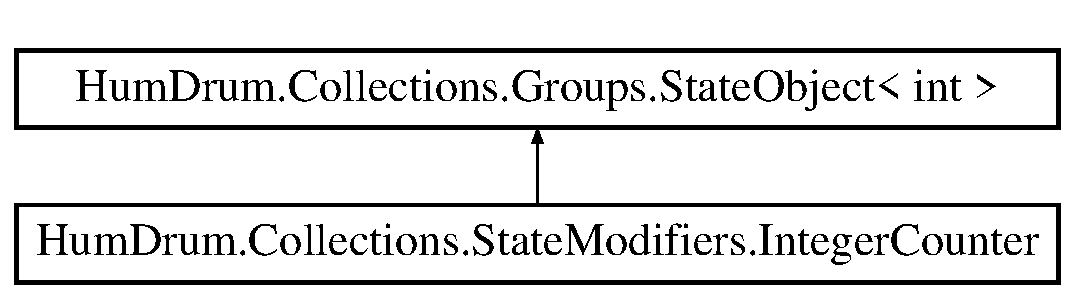
\includegraphics[height=2.000000cm]{classHumDrum_1_1Collections_1_1StateModifiers_1_1IntegerCounter}
\end{center}
\end{figure}
\subsection*{Public Member Functions}
\begin{DoxyCompactItemize}
\item 
\hyperlink{classHumDrum_1_1Collections_1_1StateModifiers_1_1IntegerCounter_aaea0c5cd68fb791212431fe814da3b78}{Integer\+Counter} (int cap, int increase\+By)
\begin{DoxyCompactList}\small\item\em Initializes a new instance of the \hyperlink{classHumDrum_1_1Collections_1_1StateModifiers_1_1IntegerCounter}{Hum\+Drum.\+Collections.\+State\+Modifiers.\+Integer\+Counter} class. \char`\"{}cap\char`\"{} is how high you wish to count to (from 0). increase\+By is how much each iteration should increase the State by. \end{DoxyCompactList}\item 
override void \hyperlink{classHumDrum_1_1Collections_1_1StateModifiers_1_1IntegerCounter_a8723ab8842f09ee98d9e13b7714d14a7}{Reset} ()
\begin{DoxyCompactList}\small\item\em Reset this state \end{DoxyCompactList}\end{DoxyCompactItemize}
\subsection*{Additional Inherited Members}


\subsection{Detailed Description}
A state machine used to count to a certain integer 



Definition at line 9 of file Integer\+Counter.\+cs.



\subsection{Constructor \& Destructor Documentation}
\index{Hum\+Drum\+::\+Collections\+::\+State\+Modifiers\+::\+Integer\+Counter@{Hum\+Drum\+::\+Collections\+::\+State\+Modifiers\+::\+Integer\+Counter}!Integer\+Counter@{Integer\+Counter}}
\index{Integer\+Counter@{Integer\+Counter}!Hum\+Drum\+::\+Collections\+::\+State\+Modifiers\+::\+Integer\+Counter@{Hum\+Drum\+::\+Collections\+::\+State\+Modifiers\+::\+Integer\+Counter}}
\subsubsection[{\texorpdfstring{Integer\+Counter(int cap, int increase\+By)}{IntegerCounter(int cap, int increaseBy)}}]{\setlength{\rightskip}{0pt plus 5cm}Hum\+Drum.\+Collections.\+State\+Modifiers.\+Integer\+Counter.\+Integer\+Counter (
\begin{DoxyParamCaption}
\item[{int}]{cap, }
\item[{int}]{increase\+By}
\end{DoxyParamCaption}
)\hspace{0.3cm}{\ttfamily [inline]}}\hypertarget{classHumDrum_1_1Collections_1_1StateModifiers_1_1IntegerCounter_aaea0c5cd68fb791212431fe814da3b78}{}\label{classHumDrum_1_1Collections_1_1StateModifiers_1_1IntegerCounter_aaea0c5cd68fb791212431fe814da3b78}


Initializes a new instance of the \hyperlink{classHumDrum_1_1Collections_1_1StateModifiers_1_1IntegerCounter}{Hum\+Drum.\+Collections.\+State\+Modifiers.\+Integer\+Counter} class. \char`\"{}cap\char`\"{} is how high you wish to count to (from 0). increase\+By is how much each iteration should increase the State by. 


\begin{DoxyParams}{Parameters}
{\em cap} & The threshold value\\
\hline
{\em increase\+By} & The interative step\\
\hline
\end{DoxyParams}


Definition at line 18 of file Integer\+Counter.\+cs.



\subsection{Member Function Documentation}
\index{Hum\+Drum\+::\+Collections\+::\+State\+Modifiers\+::\+Integer\+Counter@{Hum\+Drum\+::\+Collections\+::\+State\+Modifiers\+::\+Integer\+Counter}!Reset@{Reset}}
\index{Reset@{Reset}!Hum\+Drum\+::\+Collections\+::\+State\+Modifiers\+::\+Integer\+Counter@{Hum\+Drum\+::\+Collections\+::\+State\+Modifiers\+::\+Integer\+Counter}}
\subsubsection[{\texorpdfstring{Reset()}{Reset()}}]{\setlength{\rightskip}{0pt plus 5cm}override void Hum\+Drum.\+Collections.\+State\+Modifiers.\+Integer\+Counter.\+Reset (
\begin{DoxyParamCaption}
{}
\end{DoxyParamCaption}
)\hspace{0.3cm}{\ttfamily [inline]}, {\ttfamily [virtual]}}\hypertarget{classHumDrum_1_1Collections_1_1StateModifiers_1_1IntegerCounter_a8723ab8842f09ee98d9e13b7714d14a7}{}\label{classHumDrum_1_1Collections_1_1StateModifiers_1_1IntegerCounter_a8723ab8842f09ee98d9e13b7714d14a7}


Reset this state 



Reimplemented from \hyperlink{classHumDrum_1_1Collections_1_1Groups_1_1StateObject_aecd06a8d2511a91f5b1422c8fe3836b2}{Hum\+Drum.\+Collections.\+Groups.\+State\+Object$<$ int $>$}.



Definition at line 29 of file Integer\+Counter.\+cs.



The documentation for this class was generated from the following file\+:\begin{DoxyCompactItemize}
\item 
Hum\+Drum/\+Hum\+Drum/\+Collections/\+State\+Modifiers/Integer\+Counter.\+cs\end{DoxyCompactItemize}

\hypertarget{classHumDrum_1_1Traits_1_1Interface}{}\section{Hum\+Drum.\+Traits.\+Interface Class Reference}
\label{classHumDrum_1_1Traits_1_1Interface}\index{Hum\+Drum.\+Traits.\+Interface@{Hum\+Drum.\+Traits.\+Interface}}


Represents an interface  


\subsection*{Public Member Functions}
\begin{DoxyCompactItemize}
\item 
\hyperlink{classHumDrum_1_1Traits_1_1Interface_a71ea0b76df521bd6a3980b7cbdfe7bda}{Interface} (Type type)
\begin{DoxyCompactList}\small\item\em Initializes a new instance of the \hyperlink{classHumDrum_1_1Traits_1_1Interface}{Hum\+Drum.\+Traits.\+Interface} class. This will ensure that this type is an interface \end{DoxyCompactList}\item 
I\+Enumerable$<$ \hyperlink{classHumDrum_1_1Traits_1_1Method}{Method} $>$ \hyperlink{classHumDrum_1_1Traits_1_1Interface_a8804cbfd180dd33d913f30057db2b56a}{Methods} ()
\begin{DoxyCompactList}\small\item\em Returns the Methods that this \hyperlink{classHumDrum_1_1Traits_1_1Interface}{Interface} has. \end{DoxyCompactList}\end{DoxyCompactItemize}
\subsection*{Properties}
\begin{DoxyCompactItemize}
\item 
Type \hyperlink{classHumDrum_1_1Traits_1_1Interface_a027e973a547e202a2af1b34c2e5bc868}{Basic\+Type}\hspace{0.3cm}{\ttfamily  \mbox{[}get\mbox{]}}
\begin{DoxyCompactList}\small\item\em The \hyperlink{classHumDrum_1_1Traits_1_1Interface}{Interface}, held here as a Type \end{DoxyCompactList}\end{DoxyCompactItemize}


\subsection{Detailed Description}
Represents an interface 



Definition at line 10 of file Interface.\+cs.



\subsection{Constructor \& Destructor Documentation}
\hypertarget{classHumDrum_1_1Traits_1_1Interface_a71ea0b76df521bd6a3980b7cbdfe7bda}{}\index{Hum\+Drum\+::\+Traits\+::\+Interface@{Hum\+Drum\+::\+Traits\+::\+Interface}!Interface@{Interface}}
\index{Interface@{Interface}!Hum\+Drum\+::\+Traits\+::\+Interface@{Hum\+Drum\+::\+Traits\+::\+Interface}}
\subsubsection[{Interface(\+Type type)}]{\setlength{\rightskip}{0pt plus 5cm}Hum\+Drum.\+Traits.\+Interface.\+Interface (
\begin{DoxyParamCaption}
\item[{Type}]{type}
\end{DoxyParamCaption}
)\hspace{0.3cm}{\ttfamily [inline]}}\label{classHumDrum_1_1Traits_1_1Interface_a71ea0b76df521bd6a3980b7cbdfe7bda}


Initializes a new instance of the \hyperlink{classHumDrum_1_1Traits_1_1Interface}{Hum\+Drum.\+Traits.\+Interface} class. This will ensure that this type is an interface 


\begin{DoxyParams}{Parameters}
{\em type} & The type to attempt to initialize\\
\hline
\end{DoxyParams}


Definition at line 23 of file Interface.\+cs.



\subsection{Member Function Documentation}
\hypertarget{classHumDrum_1_1Traits_1_1Interface_a8804cbfd180dd33d913f30057db2b56a}{}\index{Hum\+Drum\+::\+Traits\+::\+Interface@{Hum\+Drum\+::\+Traits\+::\+Interface}!Methods@{Methods}}
\index{Methods@{Methods}!Hum\+Drum\+::\+Traits\+::\+Interface@{Hum\+Drum\+::\+Traits\+::\+Interface}}
\subsubsection[{Methods()}]{\setlength{\rightskip}{0pt plus 5cm}I\+Enumerable$<${\bf Method}$>$ Hum\+Drum.\+Traits.\+Interface.\+Methods (
\begin{DoxyParamCaption}
{}
\end{DoxyParamCaption}
)\hspace{0.3cm}{\ttfamily [inline]}}\label{classHumDrum_1_1Traits_1_1Interface_a8804cbfd180dd33d913f30057db2b56a}


Returns the Methods that this \hyperlink{classHumDrum_1_1Traits_1_1Interface}{Interface} has. 



Definition at line 33 of file Interface.\+cs.



\subsection{Property Documentation}
\hypertarget{classHumDrum_1_1Traits_1_1Interface_a027e973a547e202a2af1b34c2e5bc868}{}\index{Hum\+Drum\+::\+Traits\+::\+Interface@{Hum\+Drum\+::\+Traits\+::\+Interface}!Basic\+Type@{Basic\+Type}}
\index{Basic\+Type@{Basic\+Type}!Hum\+Drum\+::\+Traits\+::\+Interface@{Hum\+Drum\+::\+Traits\+::\+Interface}}
\subsubsection[{Basic\+Type}]{\setlength{\rightskip}{0pt plus 5cm}Type Hum\+Drum.\+Traits.\+Interface.\+Basic\+Type\hspace{0.3cm}{\ttfamily [get]}}\label{classHumDrum_1_1Traits_1_1Interface_a027e973a547e202a2af1b34c2e5bc868}


The \hyperlink{classHumDrum_1_1Traits_1_1Interface}{Interface}, held here as a Type 

The basic type

Definition at line 16 of file Interface.\+cs.



The documentation for this class was generated from the following file\+:\begin{DoxyCompactItemize}
\item 
Hum\+Drum/\+Hum\+Drum/\+Traits/Interface.\+cs\end{DoxyCompactItemize}

\hypertarget{interfaceHumDrum_1_1Operations_1_1Files_1_1ISequentialWriter}{}\section{Hum\+Drum.\+Operations.\+Files.\+I\+Sequential\+Writer Interface Reference}
\label{interfaceHumDrum_1_1Operations_1_1Files_1_1ISequentialWriter}\index{Hum\+Drum.\+Operations.\+Files.\+I\+Sequential\+Writer@{Hum\+Drum.\+Operations.\+Files.\+I\+Sequential\+Writer}}


Sequential writer. This will return a filename that is sequential in some way.  


Inheritance diagram for Hum\+Drum.\+Operations.\+Files.\+I\+Sequential\+Writer\+:\begin{figure}[H]
\begin{center}
\leavevmode
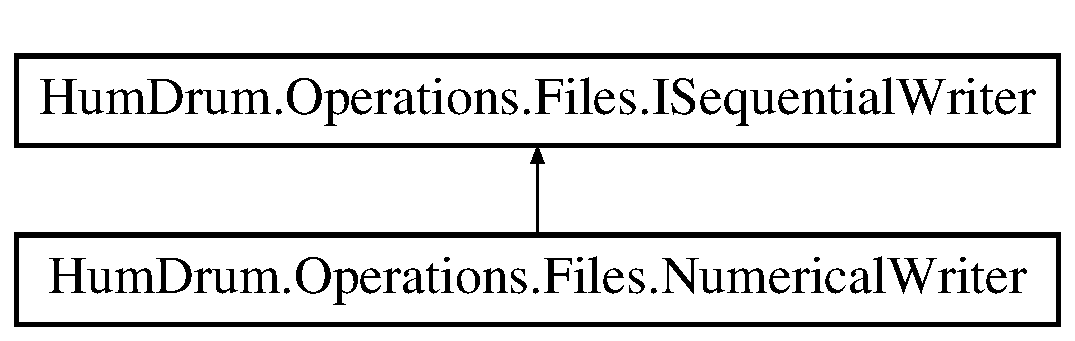
\includegraphics[height=2.000000cm]{interfaceHumDrum_1_1Operations_1_1Files_1_1ISequentialWriter}
\end{center}
\end{figure}
\subsection*{Public Member Functions}
\begin{DoxyCompactItemize}
\item 
string \hyperlink{interfaceHumDrum_1_1Operations_1_1Files_1_1ISequentialWriter_aa8afc6673f6dfcc48a30732f2a6d7fa9}{Name} (string directory, string extension)
\begin{DoxyCompactList}\small\item\em Gets the next possible name in the directory \end{DoxyCompactList}\item 
void \hyperlink{interfaceHumDrum_1_1Operations_1_1Files_1_1ISequentialWriter_ab9c1a57dd13d995dd5fdc35103071183}{Write} (string directory, string text, string extension)
\begin{DoxyCompactList}\small\item\em Write the text to the next file in the directory \end{DoxyCompactList}\end{DoxyCompactItemize}


\subsection{Detailed Description}
Sequential writer. This will return a filename that is sequential in some way. 



Definition at line 9 of file I\+Sequential\+Writer.\+cs.



\subsection{Member Function Documentation}
\index{Hum\+Drum\+::\+Operations\+::\+Files\+::\+I\+Sequential\+Writer@{Hum\+Drum\+::\+Operations\+::\+Files\+::\+I\+Sequential\+Writer}!Name@{Name}}
\index{Name@{Name}!Hum\+Drum\+::\+Operations\+::\+Files\+::\+I\+Sequential\+Writer@{Hum\+Drum\+::\+Operations\+::\+Files\+::\+I\+Sequential\+Writer}}
\subsubsection[{\texorpdfstring{Name(string directory, string extension)}{Name(string directory, string extension)}}]{\setlength{\rightskip}{0pt plus 5cm}string Hum\+Drum.\+Operations.\+Files.\+I\+Sequential\+Writer.\+Name (
\begin{DoxyParamCaption}
\item[{string}]{directory, }
\item[{string}]{extension}
\end{DoxyParamCaption}
)}\hypertarget{interfaceHumDrum_1_1Operations_1_1Files_1_1ISequentialWriter_aa8afc6673f6dfcc48a30732f2a6d7fa9}{}\label{interfaceHumDrum_1_1Operations_1_1Files_1_1ISequentialWriter_aa8afc6673f6dfcc48a30732f2a6d7fa9}


Gets the next possible name in the directory 


\begin{DoxyParams}{Parameters}
{\em directory} & The directory to analyze\\
\hline
\end{DoxyParams}


Implemented in \hyperlink{classHumDrum_1_1Operations_1_1Files_1_1NumericalWriter_a101298a93b7984f57f8f52b802e3945e}{Hum\+Drum.\+Operations.\+Files.\+Numerical\+Writer}.

\index{Hum\+Drum\+::\+Operations\+::\+Files\+::\+I\+Sequential\+Writer@{Hum\+Drum\+::\+Operations\+::\+Files\+::\+I\+Sequential\+Writer}!Write@{Write}}
\index{Write@{Write}!Hum\+Drum\+::\+Operations\+::\+Files\+::\+I\+Sequential\+Writer@{Hum\+Drum\+::\+Operations\+::\+Files\+::\+I\+Sequential\+Writer}}
\subsubsection[{\texorpdfstring{Write(string directory, string text, string extension)}{Write(string directory, string text, string extension)}}]{\setlength{\rightskip}{0pt plus 5cm}void Hum\+Drum.\+Operations.\+Files.\+I\+Sequential\+Writer.\+Write (
\begin{DoxyParamCaption}
\item[{string}]{directory, }
\item[{string}]{text, }
\item[{string}]{extension}
\end{DoxyParamCaption}
)}\hypertarget{interfaceHumDrum_1_1Operations_1_1Files_1_1ISequentialWriter_ab9c1a57dd13d995dd5fdc35103071183}{}\label{interfaceHumDrum_1_1Operations_1_1Files_1_1ISequentialWriter_ab9c1a57dd13d995dd5fdc35103071183}


Write the text to the next file in the directory 


\begin{DoxyParams}{Parameters}
{\em directory} & The directory to write in\\
\hline
{\em text} & The text to write\\
\hline
\end{DoxyParams}


Implemented in \hyperlink{classHumDrum_1_1Operations_1_1Files_1_1NumericalWriter_a27becb60062cf9556fcb4063c0baf3af}{Hum\+Drum.\+Operations.\+Files.\+Numerical\+Writer}.



The documentation for this interface was generated from the following file\+:\begin{DoxyCompactItemize}
\item 
Hum\+Drum/\+Hum\+Drum/\+Operations/\+Files/I\+Sequential\+Writer.\+cs\end{DoxyCompactItemize}

\hypertarget{classHumDrum_1_1Operations_1_1Files_1_1Line}{}\section{Hum\+Drum.\+Operations.\+Files.\+Line Class Reference}
\label{classHumDrum_1_1Operations_1_1Files_1_1Line}\index{Hum\+Drum.\+Operations.\+Files.\+Line@{Hum\+Drum.\+Operations.\+Files.\+Line}}


Class representing a line from a text file  


\subsection*{Public Member Functions}
\begin{DoxyCompactItemize}
\item 
\hyperlink{classHumDrum_1_1Operations_1_1Files_1_1Line_a0156389122d6b73dc7d12dfa3025c89c}{Line} (string text, string file, int number)
\begin{DoxyCompactList}\small\item\em Initializes a new instance of the \hyperlink{classHumDrum_1_1Operations_1_1Files_1_1Line}{Hum\+Drum.\+Operations.\+Files.\+Line} class. This uses the text from a line and the filename \end{DoxyCompactList}\end{DoxyCompactItemize}
\subsection*{Static Public Member Functions}
\begin{DoxyCompactItemize}
\item 
static I\+Enumerable$<$ \hyperlink{classHumDrum_1_1Operations_1_1Files_1_1Line}{Line} $>$ \hyperlink{classHumDrum_1_1Operations_1_1Files_1_1Line_a0e5baa7df28beb4d8549ff7a3106bf82}{All\+Lines} (string filename)
\begin{DoxyCompactList}\small\item\em Reads the lines of a file and returns a list of \hyperlink{classHumDrum_1_1Operations_1_1Files_1_1Line}{Line} objects. \end{DoxyCompactList}\end{DoxyCompactItemize}
\subsection*{Properties}
\begin{DoxyCompactItemize}
\item 
string \hyperlink{classHumDrum_1_1Operations_1_1Files_1_1Line_a885daada20e09b8b049b1804b0b44005}{Text}\hspace{0.3cm}{\ttfamily  \mbox{[}get, set\mbox{]}}
\begin{DoxyCompactList}\small\item\em The text of the line \end{DoxyCompactList}\item 
string \hyperlink{classHumDrum_1_1Operations_1_1Files_1_1Line_ac9436ae7b88a971f32d4011a7e523d26}{Filename}\hspace{0.3cm}{\ttfamily  \mbox{[}get, set\mbox{]}}
\begin{DoxyCompactList}\small\item\em The file where this line came from \end{DoxyCompactList}\item 
int \hyperlink{classHumDrum_1_1Operations_1_1Files_1_1Line_acb6f59b3bf5a85ebfb190f53d0cb7c3b}{Line\+Number}\hspace{0.3cm}{\ttfamily  \mbox{[}get, set\mbox{]}}
\begin{DoxyCompactList}\small\item\em The line number where this line occured \end{DoxyCompactList}\end{DoxyCompactItemize}


\subsection{Detailed Description}
Class representing a line from a text file 



Definition at line 11 of file Line.\+cs.



\subsection{Constructor \& Destructor Documentation}
\hypertarget{classHumDrum_1_1Operations_1_1Files_1_1Line_a0156389122d6b73dc7d12dfa3025c89c}{}\index{Hum\+Drum\+::\+Operations\+::\+Files\+::\+Line@{Hum\+Drum\+::\+Operations\+::\+Files\+::\+Line}!Line@{Line}}
\index{Line@{Line}!Hum\+Drum\+::\+Operations\+::\+Files\+::\+Line@{Hum\+Drum\+::\+Operations\+::\+Files\+::\+Line}}
\subsubsection[{Line(string text, string file, int number)}]{\setlength{\rightskip}{0pt plus 5cm}Hum\+Drum.\+Operations.\+Files.\+Line.\+Line (
\begin{DoxyParamCaption}
\item[{string}]{text, }
\item[{string}]{file, }
\item[{int}]{number}
\end{DoxyParamCaption}
)\hspace{0.3cm}{\ttfamily [inline]}}\label{classHumDrum_1_1Operations_1_1Files_1_1Line_a0156389122d6b73dc7d12dfa3025c89c}


Initializes a new instance of the \hyperlink{classHumDrum_1_1Operations_1_1Files_1_1Line}{Hum\+Drum.\+Operations.\+Files.\+Line} class. This uses the text from a line and the filename 


\begin{DoxyParams}{Parameters}
{\em text} & The text\\
\hline
{\em file} & The filename\\
\hline
{\em number} & The line number\\
\hline
\end{DoxyParams}


Definition at line 38 of file Line.\+cs.



\subsection{Member Function Documentation}
\hypertarget{classHumDrum_1_1Operations_1_1Files_1_1Line_a0e5baa7df28beb4d8549ff7a3106bf82}{}\index{Hum\+Drum\+::\+Operations\+::\+Files\+::\+Line@{Hum\+Drum\+::\+Operations\+::\+Files\+::\+Line}!All\+Lines@{All\+Lines}}
\index{All\+Lines@{All\+Lines}!Hum\+Drum\+::\+Operations\+::\+Files\+::\+Line@{Hum\+Drum\+::\+Operations\+::\+Files\+::\+Line}}
\subsubsection[{All\+Lines(string filename)}]{\setlength{\rightskip}{0pt plus 5cm}static I\+Enumerable$<${\bf Line}$>$ Hum\+Drum.\+Operations.\+Files.\+Line.\+All\+Lines (
\begin{DoxyParamCaption}
\item[{string}]{filename}
\end{DoxyParamCaption}
)\hspace{0.3cm}{\ttfamily [inline]}, {\ttfamily [static]}}\label{classHumDrum_1_1Operations_1_1Files_1_1Line_a0e5baa7df28beb4d8549ff7a3106bf82}


Reads the lines of a file and returns a list of \hyperlink{classHumDrum_1_1Operations_1_1Files_1_1Line}{Line} objects. 

\begin{DoxyReturn}{Returns}
The lines objects
\end{DoxyReturn}

\begin{DoxyParams}{Parameters}
{\em filename} & The filename to take in\\
\hline
\end{DoxyParams}


Definition at line 50 of file Line.\+cs.



\subsection{Property Documentation}
\hypertarget{classHumDrum_1_1Operations_1_1Files_1_1Line_ac9436ae7b88a971f32d4011a7e523d26}{}\index{Hum\+Drum\+::\+Operations\+::\+Files\+::\+Line@{Hum\+Drum\+::\+Operations\+::\+Files\+::\+Line}!Filename@{Filename}}
\index{Filename@{Filename}!Hum\+Drum\+::\+Operations\+::\+Files\+::\+Line@{Hum\+Drum\+::\+Operations\+::\+Files\+::\+Line}}
\subsubsection[{Filename}]{\setlength{\rightskip}{0pt plus 5cm}string Hum\+Drum.\+Operations.\+Files.\+Line.\+Filename\hspace{0.3cm}{\ttfamily [get]}, {\ttfamily [set]}}\label{classHumDrum_1_1Operations_1_1Files_1_1Line_ac9436ae7b88a971f32d4011a7e523d26}


The file where this line came from 

The filename

Definition at line 23 of file Line.\+cs.

\hypertarget{classHumDrum_1_1Operations_1_1Files_1_1Line_acb6f59b3bf5a85ebfb190f53d0cb7c3b}{}\index{Hum\+Drum\+::\+Operations\+::\+Files\+::\+Line@{Hum\+Drum\+::\+Operations\+::\+Files\+::\+Line}!Line\+Number@{Line\+Number}}
\index{Line\+Number@{Line\+Number}!Hum\+Drum\+::\+Operations\+::\+Files\+::\+Line@{Hum\+Drum\+::\+Operations\+::\+Files\+::\+Line}}
\subsubsection[{Line\+Number}]{\setlength{\rightskip}{0pt plus 5cm}int Hum\+Drum.\+Operations.\+Files.\+Line.\+Line\+Number\hspace{0.3cm}{\ttfamily [get]}, {\ttfamily [set]}}\label{classHumDrum_1_1Operations_1_1Files_1_1Line_acb6f59b3bf5a85ebfb190f53d0cb7c3b}


The line number where this line occured 

The line number

Definition at line 29 of file Line.\+cs.

\hypertarget{classHumDrum_1_1Operations_1_1Files_1_1Line_a885daada20e09b8b049b1804b0b44005}{}\index{Hum\+Drum\+::\+Operations\+::\+Files\+::\+Line@{Hum\+Drum\+::\+Operations\+::\+Files\+::\+Line}!Text@{Text}}
\index{Text@{Text}!Hum\+Drum\+::\+Operations\+::\+Files\+::\+Line@{Hum\+Drum\+::\+Operations\+::\+Files\+::\+Line}}
\subsubsection[{Text}]{\setlength{\rightskip}{0pt plus 5cm}string Hum\+Drum.\+Operations.\+Files.\+Line.\+Text\hspace{0.3cm}{\ttfamily [get]}, {\ttfamily [set]}}\label{classHumDrum_1_1Operations_1_1Files_1_1Line_a885daada20e09b8b049b1804b0b44005}


The text of the line 

The text

Definition at line 17 of file Line.\+cs.



The documentation for this class was generated from the following file\+:\begin{DoxyCompactItemize}
\item 
Hum\+Drum/\+Hum\+Drum/\+Operations/\+Files/Line.\+cs\end{DoxyCompactItemize}

\hypertarget{classHumDrum_1_1Operations_1_1Logger}{}\section{Hum\+Drum.\+Operations.\+Logger Class Reference}
\label{classHumDrum_1_1Operations_1_1Logger}\index{Hum\+Drum.\+Operations.\+Logger@{Hum\+Drum.\+Operations.\+Logger}}


\hyperlink{classHumDrum_1_1Operations_1_1Logger}{Logger} is the class responsible for logging output to a stream, which is usually a file or standard output.  


\subsection*{Public Member Functions}
\begin{DoxyCompactItemize}
\item 
\hyperlink{classHumDrum_1_1Operations_1_1Logger_af70b3833eec3d10e4db40c7e6155653f}{Logger} (Stream output\+Stream)
\begin{DoxyCompactList}\small\item\em Create a file from a stream \end{DoxyCompactList}\item 
\hyperlink{classHumDrum_1_1Operations_1_1Logger_ae14a5d07a65158c2d47e6fd30eeed3c5}{Logger} (string path)
\begin{DoxyCompactList}\small\item\em Create a logger with a specified file as its output stream. \end{DoxyCompactList}\item 
void \hyperlink{classHumDrum_1_1Operations_1_1Logger_aa3262d454bca40fcaa50f9efe40f4ecf}{Log\+Raw} (string data)
\begin{DoxyCompactList}\small\item\em Log a piece of data in its raw, exact format \end{DoxyCompactList}\item 
void \hyperlink{classHumDrum_1_1Operations_1_1Logger_a104c5e6b818bf0c33c9c3f2b6e5a5b35}{Log} (string data, Date\+Time time)
\begin{DoxyCompactList}\small\item\em Log a particular moment in time \end{DoxyCompactList}\item 
void \hyperlink{classHumDrum_1_1Operations_1_1Logger_ad29203e9bf7246a3ee8bef90efa558e6}{Log} (string data)
\begin{DoxyCompactList}\small\item\em Log the data, using the current time as the timestamp \end{DoxyCompactList}\item 
void \hyperlink{classHumDrum_1_1Operations_1_1Logger_a517acdd22bdcc327bf508623e0c921a4}{Warn} (string data)
\begin{DoxyCompactList}\small\item\em Create a warning with the given data \end{DoxyCompactList}\end{DoxyCompactItemize}


\subsection{Detailed Description}
\hyperlink{classHumDrum_1_1Operations_1_1Logger}{Logger} is the class responsible for logging output to a stream, which is usually a file or standard output. 



Definition at line 10 of file Logger.\+cs.



\subsection{Constructor \& Destructor Documentation}
\hypertarget{classHumDrum_1_1Operations_1_1Logger_af70b3833eec3d10e4db40c7e6155653f}{}\index{Hum\+Drum\+::\+Operations\+::\+Logger@{Hum\+Drum\+::\+Operations\+::\+Logger}!Logger@{Logger}}
\index{Logger@{Logger}!Hum\+Drum\+::\+Operations\+::\+Logger@{Hum\+Drum\+::\+Operations\+::\+Logger}}
\subsubsection[{Logger(\+Stream output\+Stream)}]{\setlength{\rightskip}{0pt plus 5cm}Hum\+Drum.\+Operations.\+Logger.\+Logger (
\begin{DoxyParamCaption}
\item[{Stream}]{output\+Stream}
\end{DoxyParamCaption}
)\hspace{0.3cm}{\ttfamily [inline]}}\label{classHumDrum_1_1Operations_1_1Logger_af70b3833eec3d10e4db40c7e6155653f}


Create a file from a stream 


\begin{DoxyParams}{Parameters}
{\em output\+Stream} & Any stream. Usually Standard\+Output or a file stream\\
\hline
\end{DoxyParams}


Definition at line 21 of file Logger.\+cs.

\hypertarget{classHumDrum_1_1Operations_1_1Logger_ae14a5d07a65158c2d47e6fd30eeed3c5}{}\index{Hum\+Drum\+::\+Operations\+::\+Logger@{Hum\+Drum\+::\+Operations\+::\+Logger}!Logger@{Logger}}
\index{Logger@{Logger}!Hum\+Drum\+::\+Operations\+::\+Logger@{Hum\+Drum\+::\+Operations\+::\+Logger}}
\subsubsection[{Logger(string path)}]{\setlength{\rightskip}{0pt plus 5cm}Hum\+Drum.\+Operations.\+Logger.\+Logger (
\begin{DoxyParamCaption}
\item[{string}]{path}
\end{DoxyParamCaption}
)\hspace{0.3cm}{\ttfamily [inline]}}\label{classHumDrum_1_1Operations_1_1Logger_ae14a5d07a65158c2d47e6fd30eeed3c5}


Create a logger with a specified file as its output stream. 


\begin{DoxyParams}{Parameters}
{\em log\+File} & The path to the file to write to\\
\hline
\end{DoxyParams}


Definition at line 30 of file Logger.\+cs.



\subsection{Member Function Documentation}
\hypertarget{classHumDrum_1_1Operations_1_1Logger_a104c5e6b818bf0c33c9c3f2b6e5a5b35}{}\index{Hum\+Drum\+::\+Operations\+::\+Logger@{Hum\+Drum\+::\+Operations\+::\+Logger}!Log@{Log}}
\index{Log@{Log}!Hum\+Drum\+::\+Operations\+::\+Logger@{Hum\+Drum\+::\+Operations\+::\+Logger}}
\subsubsection[{Log(string data, Date\+Time time)}]{\setlength{\rightskip}{0pt plus 5cm}void Hum\+Drum.\+Operations.\+Logger.\+Log (
\begin{DoxyParamCaption}
\item[{string}]{data, }
\item[{Date\+Time}]{time}
\end{DoxyParamCaption}
)\hspace{0.3cm}{\ttfamily [inline]}}\label{classHumDrum_1_1Operations_1_1Logger_a104c5e6b818bf0c33c9c3f2b6e5a5b35}


Log a particular moment in time 


\begin{DoxyParams}{Parameters}
{\em data} & The data to write to the log\\
\hline
{\em time} & The time to use for the timestamp\\
\hline
\end{DoxyParams}


Definition at line 49 of file Logger.\+cs.

\hypertarget{classHumDrum_1_1Operations_1_1Logger_ad29203e9bf7246a3ee8bef90efa558e6}{}\index{Hum\+Drum\+::\+Operations\+::\+Logger@{Hum\+Drum\+::\+Operations\+::\+Logger}!Log@{Log}}
\index{Log@{Log}!Hum\+Drum\+::\+Operations\+::\+Logger@{Hum\+Drum\+::\+Operations\+::\+Logger}}
\subsubsection[{Log(string data)}]{\setlength{\rightskip}{0pt plus 5cm}void Hum\+Drum.\+Operations.\+Logger.\+Log (
\begin{DoxyParamCaption}
\item[{string}]{data}
\end{DoxyParamCaption}
)\hspace{0.3cm}{\ttfamily [inline]}}\label{classHumDrum_1_1Operations_1_1Logger_ad29203e9bf7246a3ee8bef90efa558e6}


Log the data, using the current time as the timestamp 


\begin{DoxyParams}{Parameters}
{\em data} & The data to write to the log file\\
\hline
\end{DoxyParams}


Definition at line 57 of file Logger.\+cs.

\hypertarget{classHumDrum_1_1Operations_1_1Logger_aa3262d454bca40fcaa50f9efe40f4ecf}{}\index{Hum\+Drum\+::\+Operations\+::\+Logger@{Hum\+Drum\+::\+Operations\+::\+Logger}!Log\+Raw@{Log\+Raw}}
\index{Log\+Raw@{Log\+Raw}!Hum\+Drum\+::\+Operations\+::\+Logger@{Hum\+Drum\+::\+Operations\+::\+Logger}}
\subsubsection[{Log\+Raw(string data)}]{\setlength{\rightskip}{0pt plus 5cm}void Hum\+Drum.\+Operations.\+Logger.\+Log\+Raw (
\begin{DoxyParamCaption}
\item[{string}]{data}
\end{DoxyParamCaption}
)\hspace{0.3cm}{\ttfamily [inline]}}\label{classHumDrum_1_1Operations_1_1Logger_aa3262d454bca40fcaa50f9efe40f4ecf}


Log a piece of data in its raw, exact format 


\begin{DoxyParams}{Parameters}
{\em data} & The data to log to the output stream\\
\hline
\end{DoxyParams}


Definition at line 38 of file Logger.\+cs.

\hypertarget{classHumDrum_1_1Operations_1_1Logger_a517acdd22bdcc327bf508623e0c921a4}{}\index{Hum\+Drum\+::\+Operations\+::\+Logger@{Hum\+Drum\+::\+Operations\+::\+Logger}!Warn@{Warn}}
\index{Warn@{Warn}!Hum\+Drum\+::\+Operations\+::\+Logger@{Hum\+Drum\+::\+Operations\+::\+Logger}}
\subsubsection[{Warn(string data)}]{\setlength{\rightskip}{0pt plus 5cm}void Hum\+Drum.\+Operations.\+Logger.\+Warn (
\begin{DoxyParamCaption}
\item[{string}]{data}
\end{DoxyParamCaption}
)\hspace{0.3cm}{\ttfamily [inline]}}\label{classHumDrum_1_1Operations_1_1Logger_a517acdd22bdcc327bf508623e0c921a4}


Create a warning with the given data 


\begin{DoxyParams}{Parameters}
{\em data} & The data to warn about\\
\hline
\end{DoxyParams}


Definition at line 65 of file Logger.\+cs.



The documentation for this class was generated from the following file\+:\begin{DoxyCompactItemize}
\item 
Hum\+Drum/\+Hum\+Drum/\+Operations/Logger.\+cs\end{DoxyCompactItemize}

\hypertarget{classHumDrumTests_1_1Collections_1_1Markov_1_1Markov}{}\section{Hum\+Drum\+Tests.\+Collections.\+Markov.\+Markov Class Reference}
\label{classHumDrumTests_1_1Collections_1_1Markov_1_1Markov}\index{Hum\+Drum\+Tests.\+Collections.\+Markov.\+Markov@{Hum\+Drum\+Tests.\+Collections.\+Markov.\+Markov}}


This class contains the unit tests for the entirety of the \hyperlink{classHumDrumTests_1_1Collections_1_1Markov_1_1Markov}{Markov} namespace. This is because Markov\+State is used as a struct, and in future versions of \hyperlink{namespaceHumDrum}{Hum\+Drum} may actually be implemented as such.  


\subsection*{Public Member Functions}
\begin{DoxyCompactItemize}
\item 
void {\bfseries Setup} ()\hypertarget{classHumDrumTests_1_1Collections_1_1Markov_1_1Markov_a84cfa4f299f032a569531b9a541fc2f2}{}\label{classHumDrumTests_1_1Collections_1_1Markov_1_1Markov_a84cfa4f299f032a569531b9a541fc2f2}

\item 
void \hyperlink{classHumDrumTests_1_1Collections_1_1Markov_1_1Markov_af19a1b51ebd34fe449607616524b737b}{Test\+Initialization} (int degree)
\begin{DoxyCompactList}\small\item\em Tests the initialization of a \hyperlink{classHumDrumTests_1_1Collections_1_1Markov_1_1Markov}{Markov} chain given a certain degree \end{DoxyCompactList}\item 
void \hyperlink{classHumDrumTests_1_1Collections_1_1Markov_1_1Markov_ae1bd8a39206beab40020a71b2293e3a0}{Test\+Initialization} ()
\begin{DoxyCompactList}\small\item\em Tests the initialization of a few degrees \end{DoxyCompactList}\item 
void \hyperlink{classHumDrumTests_1_1Collections_1_1Markov_1_1Markov_ab864cf346f0ef6e2d21ebfe14a06ecff}{Test\+Probabilities} ()
\begin{DoxyCompactList}\small\item\em Tests the probabilities that some things will occur in the \hyperlink{classHumDrumTests_1_1Collections_1_1Markov_1_1Markov}{Markov} Chain. \end{DoxyCompactList}\end{DoxyCompactItemize}


\subsection{Detailed Description}
This class contains the unit tests for the entirety of the \hyperlink{classHumDrumTests_1_1Collections_1_1Markov_1_1Markov}{Markov} namespace. This is because Markov\+State is used as a struct, and in future versions of \hyperlink{namespaceHumDrum}{Hum\+Drum} may actually be implemented as such. 



Definition at line 22 of file Markov.\+cs.



\subsection{Member Function Documentation}
\index{Hum\+Drum\+Tests\+::\+Collections\+::\+Markov\+::\+Markov@{Hum\+Drum\+Tests\+::\+Collections\+::\+Markov\+::\+Markov}!Test\+Initialization@{Test\+Initialization}}
\index{Test\+Initialization@{Test\+Initialization}!Hum\+Drum\+Tests\+::\+Collections\+::\+Markov\+::\+Markov@{Hum\+Drum\+Tests\+::\+Collections\+::\+Markov\+::\+Markov}}
\subsubsection[{\texorpdfstring{Test\+Initialization(int degree)}{TestInitialization(int degree)}}]{\setlength{\rightskip}{0pt plus 5cm}void Hum\+Drum\+Tests.\+Collections.\+Markov.\+Markov.\+Test\+Initialization (
\begin{DoxyParamCaption}
\item[{int}]{degree}
\end{DoxyParamCaption}
)\hspace{0.3cm}{\ttfamily [inline]}}\hypertarget{classHumDrumTests_1_1Collections_1_1Markov_1_1Markov_af19a1b51ebd34fe449607616524b737b}{}\label{classHumDrumTests_1_1Collections_1_1Markov_1_1Markov_af19a1b51ebd34fe449607616524b737b}


Tests the initialization of a \hyperlink{classHumDrumTests_1_1Collections_1_1Markov_1_1Markov}{Markov} chain given a certain degree 


\begin{DoxyParams}{Parameters}
{\em degree} & The degree to test\\
\hline
\end{DoxyParams}


Definition at line 44 of file Markov.\+cs.

\index{Hum\+Drum\+Tests\+::\+Collections\+::\+Markov\+::\+Markov@{Hum\+Drum\+Tests\+::\+Collections\+::\+Markov\+::\+Markov}!Test\+Initialization@{Test\+Initialization}}
\index{Test\+Initialization@{Test\+Initialization}!Hum\+Drum\+Tests\+::\+Collections\+::\+Markov\+::\+Markov@{Hum\+Drum\+Tests\+::\+Collections\+::\+Markov\+::\+Markov}}
\subsubsection[{\texorpdfstring{Test\+Initialization()}{TestInitialization()}}]{\setlength{\rightskip}{0pt plus 5cm}void Hum\+Drum\+Tests.\+Collections.\+Markov.\+Markov.\+Test\+Initialization (
\begin{DoxyParamCaption}
{}
\end{DoxyParamCaption}
)\hspace{0.3cm}{\ttfamily [inline]}}\hypertarget{classHumDrumTests_1_1Collections_1_1Markov_1_1Markov_ae1bd8a39206beab40020a71b2293e3a0}{}\label{classHumDrumTests_1_1Collections_1_1Markov_1_1Markov_ae1bd8a39206beab40020a71b2293e3a0}


Tests the initialization of a few degrees 



Definition at line 55 of file Markov.\+cs.

\index{Hum\+Drum\+Tests\+::\+Collections\+::\+Markov\+::\+Markov@{Hum\+Drum\+Tests\+::\+Collections\+::\+Markov\+::\+Markov}!Test\+Probabilities@{Test\+Probabilities}}
\index{Test\+Probabilities@{Test\+Probabilities}!Hum\+Drum\+Tests\+::\+Collections\+::\+Markov\+::\+Markov@{Hum\+Drum\+Tests\+::\+Collections\+::\+Markov\+::\+Markov}}
\subsubsection[{\texorpdfstring{Test\+Probabilities()}{TestProbabilities()}}]{\setlength{\rightskip}{0pt plus 5cm}void Hum\+Drum\+Tests.\+Collections.\+Markov.\+Markov.\+Test\+Probabilities (
\begin{DoxyParamCaption}
{}
\end{DoxyParamCaption}
)\hspace{0.3cm}{\ttfamily [inline]}}\hypertarget{classHumDrumTests_1_1Collections_1_1Markov_1_1Markov_ab864cf346f0ef6e2d21ebfe14a06ecff}{}\label{classHumDrumTests_1_1Collections_1_1Markov_1_1Markov_ab864cf346f0ef6e2d21ebfe14a06ecff}


Tests the probabilities that some things will occur in the \hyperlink{classHumDrumTests_1_1Collections_1_1Markov_1_1Markov}{Markov} Chain. 



Definition at line 66 of file Markov.\+cs.



The documentation for this class was generated from the following file\+:\begin{DoxyCompactItemize}
\item 
Hum\+Drum\+Tests/\+Collections/\+Markov/Markov.\+cs\end{DoxyCompactItemize}

\hypertarget{classHumDrum_1_1Collections_1_1Markov_1_1Markov}{}\section{Hum\+Drum.\+Collections.\+Markov.\+Markov$<$ T $>$ Class Template Reference}
\label{classHumDrum_1_1Collections_1_1Markov_1_1Markov}\index{Hum\+Drum.\+Collections.\+Markov.\+Markov$<$ T $>$@{Hum\+Drum.\+Collections.\+Markov.\+Markov$<$ T $>$}}


A representation of a markov chain for a certain type of data.  


\subsection*{Public Member Functions}
\begin{DoxyCompactItemize}
\item 
\hyperlink{classHumDrum_1_1Collections_1_1Markov_1_1Markov_ac73669b0a13f9fd1b67986167a2de447}{Markov} (I\+Enumerable$<$ T $>$ dataset, int degree)
\begin{DoxyCompactList}\small\item\em Initializes a new instance of the Hum\+Drum.\+Collections.\+Markov.\+Markov`1 class. This will automatically parse dataset into States as Markov\+States. Obviously, with a large dataset this function (neighborhood $\sim$ O(n$^\wedge$3)) will take a very long time. \end{DoxyCompactList}\item 
\hyperlink{classHumDrum_1_1Collections_1_1Markov_1_1Markov_a696a700a50647bbe73376845bbbc3d16}{Markov} (int degree)
\begin{DoxyCompactList}\small\item\em Initializes a new instance of the Hum\+Drum.\+Collections.\+Markov.\+Markov`1 class. This can initialize an instance of \hyperlink{classHumDrum_1_1Collections_1_1Markov_1_1Markov}{Markov} without a dataset. \end{DoxyCompactList}\item 
void \hyperlink{classHumDrum_1_1Collections_1_1Markov_1_1Markov_aa73e03a727cda2f9baf47941477a94cb}{Append\+Chain} (I\+Enumerable$<$ T $>$ dataset, int degree)
\begin{DoxyCompactList}\small\item\em Appends the dataset to the current markov chain \end{DoxyCompactList}\item 
double \hyperlink{classHumDrum_1_1Collections_1_1Markov_1_1Markov_aad290aa50806e24582072bfc2dfc4da0}{Probability\+Of} (I\+Enumerable$<$ T $>$ seed, T next)
\begin{DoxyCompactList}\small\item\em Finds the probability that a particular seed incurs the given state \end{DoxyCompactList}\item 
I\+Enumerable$<$ \hyperlink{classHumDrum_1_1Collections_1_1Markov_1_1MarkovState}{Markov\+State}$<$ T $>$ $>$ \hyperlink{classHumDrum_1_1Collections_1_1Markov_1_1Markov_a335512aba3225f560a44f29f39d41613}{Possibilities} (I\+Enumerable$<$ T $>$ state)
\begin{DoxyCompactList}\small\item\em Finds the possibilities given a certain state. Any \hyperlink{classHumDrum_1_1Collections_1_1Markov_1_1MarkovState}{Markov\+State} containing the state given will be returned. \end{DoxyCompactList}\item 
I\+Enumerable$<$ \hyperlink{classHumDrum_1_1Collections_1_1Markov_1_1MarkovState}{Markov\+State}$<$ T $>$ $>$ \hyperlink{classHumDrum_1_1Collections_1_1Markov_1_1Markov_aab4b626dea779625ecfcd7648f8b8d92}{By\+Likely} (I\+Enumerable$<$ T $>$ state)
\begin{DoxyCompactList}\small\item\em Return a list of Markov\+States sorted by the most likely to occur to the least likely to occur. \end{DoxyCompactList}\item 
T \hyperlink{classHumDrum_1_1Collections_1_1Markov_1_1Markov_a840ff3b5256b93f3a73b6332a237bc41}{Select\+Random} (I\+Enumerable$<$ T $>$ state)
\begin{DoxyCompactList}\small\item\em The heart of the \hyperlink{classHumDrum_1_1Collections_1_1Markov_1_1Markov}{Markov} principle. Based on the probability that each item will occur, return a random element satisfying the given state. \end{DoxyCompactList}\item 
I\+Enumerable$<$ T $>$ \hyperlink{classHumDrum_1_1Collections_1_1Markov_1_1Markov_a20d111872b9aac86b8852c1825aea822}{Select\+Random\+Sequence} (I\+Enumerable$<$ T $>$ seed, int count)
\begin{DoxyCompactList}\small\item\em Creates a sequence of randomly selected instances based on a seed and a number of items to return. \end{DoxyCompactList}\item 
I\+Enumerable$<$ T $>$ \hyperlink{classHumDrum_1_1Collections_1_1Markov_1_1Markov_a4a6b25a6f0aba3a22c8b6e183edbbd0f}{Random\+State} ()
\begin{DoxyCompactList}\small\item\em Gets a random state from the list of available states \end{DoxyCompactList}\item 
override string \hyperlink{classHumDrum_1_1Collections_1_1Markov_1_1Markov_a9386ce788662f10ba6d5cc0c7d564e29}{To\+String} ()
\begin{DoxyCompactList}\small\item\em Returns a System.\+String that represents the current Hum\+Drum.\+Collections.\+Markov.\+Markov`1. \end{DoxyCompactList}\end{DoxyCompactItemize}
\subsection*{Properties}
\begin{DoxyCompactItemize}
\item 
List$<$ \hyperlink{classHumDrum_1_1Collections_1_1Markov_1_1MarkovState}{Markov\+State}$<$ T $>$ $>$ \hyperlink{classHumDrum_1_1Collections_1_1Markov_1_1Markov_a71899515d7da8d3078ec114a7b622a5f}{States}\hspace{0.3cm}{\ttfamily  \mbox{[}get\mbox{]}}
\begin{DoxyCompactList}\small\item\em The list of states and their associated probabilities and results. \end{DoxyCompactList}\item 
int \hyperlink{classHumDrum_1_1Collections_1_1Markov_1_1Markov_a35d0586c1f941ee548203a596378da81}{Degree}\hspace{0.3cm}{\ttfamily  \mbox{[}get\mbox{]}}
\begin{DoxyCompactList}\small\item\em Gets or sets the degree of this chian \end{DoxyCompactList}\end{DoxyCompactItemize}


\subsection{Detailed Description}
A representation of a markov chain for a certain type of data. 



Definition at line 15 of file Markov.\+cs.



\subsection{Constructor \& Destructor Documentation}
\index{Hum\+Drum\+::\+Collections\+::\+Markov\+::\+Markov@{Hum\+Drum\+::\+Collections\+::\+Markov\+::\+Markov}!Markov@{Markov}}
\index{Markov@{Markov}!Hum\+Drum\+::\+Collections\+::\+Markov\+::\+Markov@{Hum\+Drum\+::\+Collections\+::\+Markov\+::\+Markov}}
\subsubsection[{\texorpdfstring{Markov(\+I\+Enumerable$<$ T $>$ dataset, int degree)}{Markov(IEnumerable< T > dataset, int degree)}}]{\setlength{\rightskip}{0pt plus 5cm}{\bf Hum\+Drum.\+Collections.\+Markov.\+Markov}$<$ T $>$.{\bf Markov} (
\begin{DoxyParamCaption}
\item[{I\+Enumerable$<$ T $>$}]{dataset, }
\item[{int}]{degree}
\end{DoxyParamCaption}
)\hspace{0.3cm}{\ttfamily [inline]}}\hypertarget{classHumDrum_1_1Collections_1_1Markov_1_1Markov_ac73669b0a13f9fd1b67986167a2de447}{}\label{classHumDrum_1_1Collections_1_1Markov_1_1Markov_ac73669b0a13f9fd1b67986167a2de447}


Initializes a new instance of the Hum\+Drum.\+Collections.\+Markov.\+Markov`1 class. This will automatically parse dataset into States as Markov\+States. Obviously, with a large dataset this function (neighborhood $\sim$ O(n$^\wedge$3)) will take a very long time. 


\begin{DoxyParams}{Parameters}
{\em dataset} & The set of data to analyze\\
\hline
{\em degree} & How many previous values define what a \char`\"{}state\char`\"{} is.\\
\hline
\end{DoxyParams}


Definition at line 38 of file Markov.\+cs.

\index{Hum\+Drum\+::\+Collections\+::\+Markov\+::\+Markov@{Hum\+Drum\+::\+Collections\+::\+Markov\+::\+Markov}!Markov@{Markov}}
\index{Markov@{Markov}!Hum\+Drum\+::\+Collections\+::\+Markov\+::\+Markov@{Hum\+Drum\+::\+Collections\+::\+Markov\+::\+Markov}}
\subsubsection[{\texorpdfstring{Markov(int degree)}{Markov(int degree)}}]{\setlength{\rightskip}{0pt plus 5cm}{\bf Hum\+Drum.\+Collections.\+Markov.\+Markov}$<$ T $>$.{\bf Markov} (
\begin{DoxyParamCaption}
\item[{int}]{degree}
\end{DoxyParamCaption}
)\hspace{0.3cm}{\ttfamily [inline]}}\hypertarget{classHumDrum_1_1Collections_1_1Markov_1_1Markov_a696a700a50647bbe73376845bbbc3d16}{}\label{classHumDrum_1_1Collections_1_1Markov_1_1Markov_a696a700a50647bbe73376845bbbc3d16}


Initializes a new instance of the Hum\+Drum.\+Collections.\+Markov.\+Markov`1 class. This can initialize an instance of \hyperlink{classHumDrum_1_1Collections_1_1Markov_1_1Markov}{Markov} without a dataset. 


\begin{DoxyParams}{Parameters}
{\em degree} & The degree of this chain\\
\hline
\end{DoxyParams}


Definition at line 51 of file Markov.\+cs.



\subsection{Member Function Documentation}
\index{Hum\+Drum\+::\+Collections\+::\+Markov\+::\+Markov@{Hum\+Drum\+::\+Collections\+::\+Markov\+::\+Markov}!Append\+Chain@{Append\+Chain}}
\index{Append\+Chain@{Append\+Chain}!Hum\+Drum\+::\+Collections\+::\+Markov\+::\+Markov@{Hum\+Drum\+::\+Collections\+::\+Markov\+::\+Markov}}
\subsubsection[{\texorpdfstring{Append\+Chain(\+I\+Enumerable$<$ T $>$ dataset, int degree)}{AppendChain(IEnumerable< T > dataset, int degree)}}]{\setlength{\rightskip}{0pt plus 5cm}void {\bf Hum\+Drum.\+Collections.\+Markov.\+Markov}$<$ T $>$.Append\+Chain (
\begin{DoxyParamCaption}
\item[{I\+Enumerable$<$ T $>$}]{dataset, }
\item[{int}]{degree}
\end{DoxyParamCaption}
)\hspace{0.3cm}{\ttfamily [inline]}}\hypertarget{classHumDrum_1_1Collections_1_1Markov_1_1Markov_aa73e03a727cda2f9baf47941477a94cb}{}\label{classHumDrum_1_1Collections_1_1Markov_1_1Markov_aa73e03a727cda2f9baf47941477a94cb}


Appends the dataset to the current markov chain 


\begin{DoxyParams}{Parameters}
{\em dataset} & The data to gather statistics from\\
\hline
{\em degree} & The degree of the markov chain\\
\hline
\end{DoxyParams}


Definition at line 62 of file Markov.\+cs.

\index{Hum\+Drum\+::\+Collections\+::\+Markov\+::\+Markov@{Hum\+Drum\+::\+Collections\+::\+Markov\+::\+Markov}!By\+Likely@{By\+Likely}}
\index{By\+Likely@{By\+Likely}!Hum\+Drum\+::\+Collections\+::\+Markov\+::\+Markov@{Hum\+Drum\+::\+Collections\+::\+Markov\+::\+Markov}}
\subsubsection[{\texorpdfstring{By\+Likely(\+I\+Enumerable$<$ T $>$ state)}{ByLikely(IEnumerable< T > state)}}]{\setlength{\rightskip}{0pt plus 5cm}I\+Enumerable$<${\bf Markov\+State}$<$T$>$ $>$ {\bf Hum\+Drum.\+Collections.\+Markov.\+Markov}$<$ T $>$.By\+Likely (
\begin{DoxyParamCaption}
\item[{I\+Enumerable$<$ T $>$}]{state}
\end{DoxyParamCaption}
)\hspace{0.3cm}{\ttfamily [inline]}}\hypertarget{classHumDrum_1_1Collections_1_1Markov_1_1Markov_aab4b626dea779625ecfcd7648f8b8d92}{}\label{classHumDrum_1_1Collections_1_1Markov_1_1Markov_aab4b626dea779625ecfcd7648f8b8d92}


Return a list of Markov\+States sorted by the most likely to occur to the least likely to occur. 

\begin{DoxyReturn}{Returns}
The likely states
\end{DoxyReturn}

\begin{DoxyParams}{Parameters}
{\em state} & The original state to start at\\
\hline
\end{DoxyParams}


Definition at line 124 of file Markov.\+cs.

\index{Hum\+Drum\+::\+Collections\+::\+Markov\+::\+Markov@{Hum\+Drum\+::\+Collections\+::\+Markov\+::\+Markov}!Possibilities@{Possibilities}}
\index{Possibilities@{Possibilities}!Hum\+Drum\+::\+Collections\+::\+Markov\+::\+Markov@{Hum\+Drum\+::\+Collections\+::\+Markov\+::\+Markov}}
\subsubsection[{\texorpdfstring{Possibilities(\+I\+Enumerable$<$ T $>$ state)}{Possibilities(IEnumerable< T > state)}}]{\setlength{\rightskip}{0pt plus 5cm}I\+Enumerable$<${\bf Markov\+State}$<$T$>$ $>$ {\bf Hum\+Drum.\+Collections.\+Markov.\+Markov}$<$ T $>$.Possibilities (
\begin{DoxyParamCaption}
\item[{I\+Enumerable$<$ T $>$}]{state}
\end{DoxyParamCaption}
)\hspace{0.3cm}{\ttfamily [inline]}}\hypertarget{classHumDrum_1_1Collections_1_1Markov_1_1Markov_a335512aba3225f560a44f29f39d41613}{}\label{classHumDrum_1_1Collections_1_1Markov_1_1Markov_a335512aba3225f560a44f29f39d41613}


Finds the possibilities given a certain state. Any \hyperlink{classHumDrum_1_1Collections_1_1Markov_1_1MarkovState}{Markov\+State} containing the state given will be returned. 


\begin{DoxyParams}{Parameters}
{\em state} & The list of states\\
\hline
\end{DoxyParams}


Definition at line 105 of file Markov.\+cs.

\index{Hum\+Drum\+::\+Collections\+::\+Markov\+::\+Markov@{Hum\+Drum\+::\+Collections\+::\+Markov\+::\+Markov}!Probability\+Of@{Probability\+Of}}
\index{Probability\+Of@{Probability\+Of}!Hum\+Drum\+::\+Collections\+::\+Markov\+::\+Markov@{Hum\+Drum\+::\+Collections\+::\+Markov\+::\+Markov}}
\subsubsection[{\texorpdfstring{Probability\+Of(\+I\+Enumerable$<$ T $>$ seed, T next)}{ProbabilityOf(IEnumerable< T > seed, T next)}}]{\setlength{\rightskip}{0pt plus 5cm}double {\bf Hum\+Drum.\+Collections.\+Markov.\+Markov}$<$ T $>$.Probability\+Of (
\begin{DoxyParamCaption}
\item[{I\+Enumerable$<$ T $>$}]{seed, }
\item[{T}]{next}
\end{DoxyParamCaption}
)\hspace{0.3cm}{\ttfamily [inline]}}\hypertarget{classHumDrum_1_1Collections_1_1Markov_1_1Markov_aad290aa50806e24582072bfc2dfc4da0}{}\label{classHumDrum_1_1Collections_1_1Markov_1_1Markov_aad290aa50806e24582072bfc2dfc4da0}


Finds the probability that a particular seed incurs the given state 

\begin{DoxyReturn}{Returns}
The probability of the event
\end{DoxyReturn}

\begin{DoxyParams}{Parameters}
{\em state} & The state to test for\\
\hline
\end{DoxyParams}


Definition at line 90 of file Markov.\+cs.

\index{Hum\+Drum\+::\+Collections\+::\+Markov\+::\+Markov@{Hum\+Drum\+::\+Collections\+::\+Markov\+::\+Markov}!Random\+State@{Random\+State}}
\index{Random\+State@{Random\+State}!Hum\+Drum\+::\+Collections\+::\+Markov\+::\+Markov@{Hum\+Drum\+::\+Collections\+::\+Markov\+::\+Markov}}
\subsubsection[{\texorpdfstring{Random\+State()}{RandomState()}}]{\setlength{\rightskip}{0pt plus 5cm}I\+Enumerable$<$T$>$ {\bf Hum\+Drum.\+Collections.\+Markov.\+Markov}$<$ T $>$.Random\+State (
\begin{DoxyParamCaption}
{}
\end{DoxyParamCaption}
)\hspace{0.3cm}{\ttfamily [inline]}}\hypertarget{classHumDrum_1_1Collections_1_1Markov_1_1Markov_a4a6b25a6f0aba3a22c8b6e183edbbd0f}{}\label{classHumDrum_1_1Collections_1_1Markov_1_1Markov_a4a6b25a6f0aba3a22c8b6e183edbbd0f}


Gets a random state from the list of available states 

\begin{DoxyReturn}{Returns}
The state
\end{DoxyReturn}


Definition at line 180 of file Markov.\+cs.

\index{Hum\+Drum\+::\+Collections\+::\+Markov\+::\+Markov@{Hum\+Drum\+::\+Collections\+::\+Markov\+::\+Markov}!Select\+Random@{Select\+Random}}
\index{Select\+Random@{Select\+Random}!Hum\+Drum\+::\+Collections\+::\+Markov\+::\+Markov@{Hum\+Drum\+::\+Collections\+::\+Markov\+::\+Markov}}
\subsubsection[{\texorpdfstring{Select\+Random(\+I\+Enumerable$<$ T $>$ state)}{SelectRandom(IEnumerable< T > state)}}]{\setlength{\rightskip}{0pt plus 5cm}T {\bf Hum\+Drum.\+Collections.\+Markov.\+Markov}$<$ T $>$.Select\+Random (
\begin{DoxyParamCaption}
\item[{I\+Enumerable$<$ T $>$}]{state}
\end{DoxyParamCaption}
)\hspace{0.3cm}{\ttfamily [inline]}}\hypertarget{classHumDrum_1_1Collections_1_1Markov_1_1Markov_a840ff3b5256b93f3a73b6332a237bc41}{}\label{classHumDrum_1_1Collections_1_1Markov_1_1Markov_a840ff3b5256b93f3a73b6332a237bc41}


The heart of the \hyperlink{classHumDrum_1_1Collections_1_1Markov_1_1Markov}{Markov} principle. Based on the probability that each item will occur, return a random element satisfying the given state. 

\begin{DoxyReturn}{Returns}
The random element
\end{DoxyReturn}

\begin{DoxyParams}{Parameters}
{\em state} & The state to be attained\\
\hline
\end{DoxyParams}


Definition at line 136 of file Markov.\+cs.

\index{Hum\+Drum\+::\+Collections\+::\+Markov\+::\+Markov@{Hum\+Drum\+::\+Collections\+::\+Markov\+::\+Markov}!Select\+Random\+Sequence@{Select\+Random\+Sequence}}
\index{Select\+Random\+Sequence@{Select\+Random\+Sequence}!Hum\+Drum\+::\+Collections\+::\+Markov\+::\+Markov@{Hum\+Drum\+::\+Collections\+::\+Markov\+::\+Markov}}
\subsubsection[{\texorpdfstring{Select\+Random\+Sequence(\+I\+Enumerable$<$ T $>$ seed, int count)}{SelectRandomSequence(IEnumerable< T > seed, int count)}}]{\setlength{\rightskip}{0pt plus 5cm}I\+Enumerable$<$T$>$ {\bf Hum\+Drum.\+Collections.\+Markov.\+Markov}$<$ T $>$.Select\+Random\+Sequence (
\begin{DoxyParamCaption}
\item[{I\+Enumerable$<$ T $>$}]{seed, }
\item[{int}]{count}
\end{DoxyParamCaption}
)\hspace{0.3cm}{\ttfamily [inline]}}\hypertarget{classHumDrum_1_1Collections_1_1Markov_1_1Markov_a20d111872b9aac86b8852c1825aea822}{}\label{classHumDrum_1_1Collections_1_1Markov_1_1Markov_a20d111872b9aac86b8852c1825aea822}


Creates a sequence of randomly selected instances based on a seed and a number of items to return. 

\begin{DoxyReturn}{Returns}
The random sequence
\end{DoxyReturn}

\begin{DoxyParams}{Parameters}
{\em seed} & The seed state\\
\hline
{\em count} & How many iterations to go\\
\hline
\end{DoxyParams}


Definition at line 162 of file Markov.\+cs.

\index{Hum\+Drum\+::\+Collections\+::\+Markov\+::\+Markov@{Hum\+Drum\+::\+Collections\+::\+Markov\+::\+Markov}!To\+String@{To\+String}}
\index{To\+String@{To\+String}!Hum\+Drum\+::\+Collections\+::\+Markov\+::\+Markov@{Hum\+Drum\+::\+Collections\+::\+Markov\+::\+Markov}}
\subsubsection[{\texorpdfstring{To\+String()}{ToString()}}]{\setlength{\rightskip}{0pt plus 5cm}override string {\bf Hum\+Drum.\+Collections.\+Markov.\+Markov}$<$ T $>$.To\+String (
\begin{DoxyParamCaption}
{}
\end{DoxyParamCaption}
)\hspace{0.3cm}{\ttfamily [inline]}}\hypertarget{classHumDrum_1_1Collections_1_1Markov_1_1Markov_a9386ce788662f10ba6d5cc0c7d564e29}{}\label{classHumDrum_1_1Collections_1_1Markov_1_1Markov_a9386ce788662f10ba6d5cc0c7d564e29}


Returns a System.\+String that represents the current Hum\+Drum.\+Collections.\+Markov.\+Markov`1. 

\begin{DoxyReturn}{Returns}
A System.\+String that represents the current Hum\+Drum.\+Collections.\+Markov.\+Markov`1.
\end{DoxyReturn}


Definition at line 189 of file Markov.\+cs.



\subsection{Property Documentation}
\index{Hum\+Drum\+::\+Collections\+::\+Markov\+::\+Markov@{Hum\+Drum\+::\+Collections\+::\+Markov\+::\+Markov}!Degree@{Degree}}
\index{Degree@{Degree}!Hum\+Drum\+::\+Collections\+::\+Markov\+::\+Markov@{Hum\+Drum\+::\+Collections\+::\+Markov\+::\+Markov}}
\subsubsection[{\texorpdfstring{Degree}{Degree}}]{\setlength{\rightskip}{0pt plus 5cm}int {\bf Hum\+Drum.\+Collections.\+Markov.\+Markov}$<$ T $>$.Degree\hspace{0.3cm}{\ttfamily [get]}}\hypertarget{classHumDrum_1_1Collections_1_1Markov_1_1Markov_a35d0586c1f941ee548203a596378da81}{}\label{classHumDrum_1_1Collections_1_1Markov_1_1Markov_a35d0586c1f941ee548203a596378da81}


Gets or sets the degree of this chian 

The degree

Definition at line 29 of file Markov.\+cs.

\index{Hum\+Drum\+::\+Collections\+::\+Markov\+::\+Markov@{Hum\+Drum\+::\+Collections\+::\+Markov\+::\+Markov}!States@{States}}
\index{States@{States}!Hum\+Drum\+::\+Collections\+::\+Markov\+::\+Markov@{Hum\+Drum\+::\+Collections\+::\+Markov\+::\+Markov}}
\subsubsection[{\texorpdfstring{States}{States}}]{\setlength{\rightskip}{0pt plus 5cm}List$<${\bf Markov\+State}$<$T$>$ $>$ {\bf Hum\+Drum.\+Collections.\+Markov.\+Markov}$<$ T $>$.States\hspace{0.3cm}{\ttfamily [get]}}\hypertarget{classHumDrum_1_1Collections_1_1Markov_1_1Markov_a71899515d7da8d3078ec114a7b622a5f}{}\label{classHumDrum_1_1Collections_1_1Markov_1_1Markov_a71899515d7da8d3078ec114a7b622a5f}


The list of states and their associated probabilities and results. 

The states

Definition at line 23 of file Markov.\+cs.



The documentation for this class was generated from the following file\+:\begin{DoxyCompactItemize}
\item 
Hum\+Drum/\+Hum\+Drum/\+Collections/\+Markov/Markov.\+cs\end{DoxyCompactItemize}

\hypertarget{classHumDrum_1_1Collections_1_1Markov_1_1MarkovState}{}\section{Hum\+Drum.\+Collections.\+Markov.\+Markov\+State$<$ T $>$ Class Template Reference}
\label{classHumDrum_1_1Collections_1_1Markov_1_1MarkovState}\index{Hum\+Drum.\+Collections.\+Markov.\+Markov\+State$<$ T $>$@{Hum\+Drum.\+Collections.\+Markov.\+Markov\+State$<$ T $>$}}


Contains information pertaining to the state of one item within a markov chain.  


\subsection*{Public Member Functions}
\begin{DoxyCompactItemize}
\item 
\hyperlink{classHumDrum_1_1Collections_1_1Markov_1_1MarkovState_a9a0ab2d8e1f4e31c3317af0fe81251bf}{Markov\+State} (I\+Enumerable$<$ T $>$ state, T next)
\begin{DoxyCompactList}\small\item\em Initializes a new instance of the Hum\+Drum.\+Collections.\+Markov.\+Markov\+State`1 class. This will set the probability to 0.\+00 so that another process can set it \end{DoxyCompactList}\item 
\hyperlink{classHumDrum_1_1Collections_1_1Markov_1_1MarkovState_a710de5d361e56453e7c57c7597eb600d}{Markov\+State} (I\+Enumerable$<$ T $>$ state, T next, double probability)
\begin{DoxyCompactList}\small\item\em Initializes a new instance of the Hum\+Drum.\+Collections.\+Markov.\+Markov\+State`1 class. If you already know the probability that something will occur, use this constructor instead \end{DoxyCompactList}\end{DoxyCompactItemize}
\subsection*{Properties}
\begin{DoxyCompactItemize}
\item 
I\+Enumerable$<$ T $>$ \hyperlink{classHumDrum_1_1Collections_1_1Markov_1_1MarkovState_a6af42036b04d84e26d06ee5d86790094}{State}\hspace{0.3cm}{\ttfamily  \mbox{[}get, set\mbox{]}}
\begin{DoxyCompactList}\small\item\em The state, of variable degree, which must be attained in order for Next to be considered. \end{DoxyCompactList}\item 
T \hyperlink{classHumDrum_1_1Collections_1_1Markov_1_1MarkovState_a825a800c1e4b27746aeb672b49e0b57b}{Next}\hspace{0.3cm}{\ttfamily  \mbox{[}get, set\mbox{]}}
\begin{DoxyCompactList}\small\item\em The item, that if State is reached, will be considered for return. \end{DoxyCompactList}\item 
double \hyperlink{classHumDrum_1_1Collections_1_1Markov_1_1MarkovState_afd0a085ed23c8922067ac105af054c34}{Probability}\hspace{0.3cm}{\ttfamily  \mbox{[}get, set\mbox{]}}
\begin{DoxyCompactList}\small\item\em The probability that, given a state is reached, the \char`\"{}\+Next\char`\"{} value will be returned \end{DoxyCompactList}\end{DoxyCompactItemize}


\subsection{Detailed Description}
Contains information pertaining to the state of one item within a markov chain. 



Definition at line 10 of file Markov\+State.\+cs.



\subsection{Constructor \& Destructor Documentation}
\hypertarget{classHumDrum_1_1Collections_1_1Markov_1_1MarkovState_a9a0ab2d8e1f4e31c3317af0fe81251bf}{}\index{Hum\+Drum\+::\+Collections\+::\+Markov\+::\+Markov\+State@{Hum\+Drum\+::\+Collections\+::\+Markov\+::\+Markov\+State}!Markov\+State@{Markov\+State}}
\index{Markov\+State@{Markov\+State}!Hum\+Drum\+::\+Collections\+::\+Markov\+::\+Markov\+State@{Hum\+Drum\+::\+Collections\+::\+Markov\+::\+Markov\+State}}
\subsubsection[{Markov\+State(\+I\+Enumerable$<$ T $>$ state, T next)}]{\setlength{\rightskip}{0pt plus 5cm}{\bf Hum\+Drum.\+Collections.\+Markov.\+Markov\+State}$<$ T $>$.{\bf Markov\+State} (
\begin{DoxyParamCaption}
\item[{I\+Enumerable$<$ T $>$}]{state, }
\item[{T}]{next}
\end{DoxyParamCaption}
)\hspace{0.3cm}{\ttfamily [inline]}}\label{classHumDrum_1_1Collections_1_1Markov_1_1MarkovState_a9a0ab2d8e1f4e31c3317af0fe81251bf}


Initializes a new instance of the Hum\+Drum.\+Collections.\+Markov.\+Markov\+State`1 class. This will set the probability to 0.\+00 so that another process can set it 


\begin{DoxyParams}{Parameters}
{\em state} & State.\\
\hline
{\em next} & Next.\\
\hline
\end{DoxyParams}


Definition at line 39 of file Markov\+State.\+cs.

\hypertarget{classHumDrum_1_1Collections_1_1Markov_1_1MarkovState_a710de5d361e56453e7c57c7597eb600d}{}\index{Hum\+Drum\+::\+Collections\+::\+Markov\+::\+Markov\+State@{Hum\+Drum\+::\+Collections\+::\+Markov\+::\+Markov\+State}!Markov\+State@{Markov\+State}}
\index{Markov\+State@{Markov\+State}!Hum\+Drum\+::\+Collections\+::\+Markov\+::\+Markov\+State@{Hum\+Drum\+::\+Collections\+::\+Markov\+::\+Markov\+State}}
\subsubsection[{Markov\+State(\+I\+Enumerable$<$ T $>$ state, T next, double probability)}]{\setlength{\rightskip}{0pt plus 5cm}{\bf Hum\+Drum.\+Collections.\+Markov.\+Markov\+State}$<$ T $>$.{\bf Markov\+State} (
\begin{DoxyParamCaption}
\item[{I\+Enumerable$<$ T $>$}]{state, }
\item[{T}]{next, }
\item[{double}]{probability}
\end{DoxyParamCaption}
)\hspace{0.3cm}{\ttfamily [inline]}}\label{classHumDrum_1_1Collections_1_1Markov_1_1MarkovState_a710de5d361e56453e7c57c7597eb600d}


Initializes a new instance of the Hum\+Drum.\+Collections.\+Markov.\+Markov\+State`1 class. If you already know the probability that something will occur, use this constructor instead 


\begin{DoxyParams}{Parameters}
{\em state} & The state of this instance\\
\hline
{\em next} & The future state of this instance\\
\hline
{\em probability} & The probability for this to occur\\
\hline
\end{DoxyParams}


Definition at line 53 of file Markov\+State.\+cs.



\subsection{Property Documentation}
\hypertarget{classHumDrum_1_1Collections_1_1Markov_1_1MarkovState_a825a800c1e4b27746aeb672b49e0b57b}{}\index{Hum\+Drum\+::\+Collections\+::\+Markov\+::\+Markov\+State@{Hum\+Drum\+::\+Collections\+::\+Markov\+::\+Markov\+State}!Next@{Next}}
\index{Next@{Next}!Hum\+Drum\+::\+Collections\+::\+Markov\+::\+Markov\+State@{Hum\+Drum\+::\+Collections\+::\+Markov\+::\+Markov\+State}}
\subsubsection[{Next}]{\setlength{\rightskip}{0pt plus 5cm}T {\bf Hum\+Drum.\+Collections.\+Markov.\+Markov\+State}$<$ T $>$.Next\hspace{0.3cm}{\ttfamily [get]}, {\ttfamily [set]}}\label{classHumDrum_1_1Collections_1_1Markov_1_1MarkovState_a825a800c1e4b27746aeb672b49e0b57b}


The item, that if State is reached, will be considered for return. 

The future value

Definition at line 24 of file Markov\+State.\+cs.

\hypertarget{classHumDrum_1_1Collections_1_1Markov_1_1MarkovState_afd0a085ed23c8922067ac105af054c34}{}\index{Hum\+Drum\+::\+Collections\+::\+Markov\+::\+Markov\+State@{Hum\+Drum\+::\+Collections\+::\+Markov\+::\+Markov\+State}!Probability@{Probability}}
\index{Probability@{Probability}!Hum\+Drum\+::\+Collections\+::\+Markov\+::\+Markov\+State@{Hum\+Drum\+::\+Collections\+::\+Markov\+::\+Markov\+State}}
\subsubsection[{Probability}]{\setlength{\rightskip}{0pt plus 5cm}double {\bf Hum\+Drum.\+Collections.\+Markov.\+Markov\+State}$<$ T $>$.Probability\hspace{0.3cm}{\ttfamily [get]}, {\ttfamily [set]}}\label{classHumDrum_1_1Collections_1_1Markov_1_1MarkovState_afd0a085ed23c8922067ac105af054c34}


The probability that, given a state is reached, the \char`\"{}\+Next\char`\"{} value will be returned 

The probability to occur

Definition at line 31 of file Markov\+State.\+cs.

\hypertarget{classHumDrum_1_1Collections_1_1Markov_1_1MarkovState_a6af42036b04d84e26d06ee5d86790094}{}\index{Hum\+Drum\+::\+Collections\+::\+Markov\+::\+Markov\+State@{Hum\+Drum\+::\+Collections\+::\+Markov\+::\+Markov\+State}!State@{State}}
\index{State@{State}!Hum\+Drum\+::\+Collections\+::\+Markov\+::\+Markov\+State@{Hum\+Drum\+::\+Collections\+::\+Markov\+::\+Markov\+State}}
\subsubsection[{State}]{\setlength{\rightskip}{0pt plus 5cm}I\+Enumerable$<$T$>$ {\bf Hum\+Drum.\+Collections.\+Markov.\+Markov\+State}$<$ T $>$.State\hspace{0.3cm}{\ttfamily [get]}, {\ttfamily [set]}}\label{classHumDrum_1_1Collections_1_1Markov_1_1MarkovState_a6af42036b04d84e26d06ee5d86790094}


The state, of variable degree, which must be attained in order for Next to be considered. 

The necessary state

Definition at line 17 of file Markov\+State.\+cs.



The documentation for this class was generated from the following file\+:\begin{DoxyCompactItemize}
\item 
Hum\+Drum/\+Hum\+Drum/\+Collections/\+Markov/Markov\+State.\+cs\end{DoxyCompactItemize}

\hypertarget{classHumDrum_1_1Traits_1_1Method}{}\section{Hum\+Drum.\+Traits.\+Method Class Reference}
\label{classHumDrum_1_1Traits_1_1Method}\index{Hum\+Drum.\+Traits.\+Method@{Hum\+Drum.\+Traits.\+Method}}


Represents a C\# \hyperlink{classHumDrum_1_1Traits_1_1Method}{Method}, based only on return values and parameter types  


\subsection*{Public Member Functions}
\begin{DoxyCompactItemize}
\item 
\hyperlink{classHumDrum_1_1Traits_1_1Method_a459d9bc4db6e1d1572d1f34fb92c19d1}{Method} (Method\+Info method)
\begin{DoxyCompactList}\small\item\em Initializes a new instance of the \hyperlink{classHumDrum_1_1Traits_1_1Method}{Hum\+Drum.\+Traits.\+Method} class. \end{DoxyCompactList}\item 
\hyperlink{classHumDrum_1_1Traits_1_1Method_ac822929c7b6871193f958fcd223e2693}{Method} (Method\+Info method, string name)
\begin{DoxyCompactList}\small\item\em Initializes a new instance of the \hyperlink{classHumDrum_1_1Traits_1_1Method}{Hum\+Drum.\+Traits.\+Method} class. This will rename the method given a Name as a String. The Basic\+Method will still contain the name of its own member, however. \end{DoxyCompactList}\item 
Type \hyperlink{classHumDrum_1_1Traits_1_1Method_af33783f5c6033774bcba1e5900e760be}{Get\+Return\+Type} ()
\begin{DoxyCompactList}\small\item\em Gets the return type of this method \end{DoxyCompactList}\item 
I\+Enumerable$<$ Type $>$ \hyperlink{classHumDrum_1_1Traits_1_1Method_a320f9c87cdb137fca994215039c03904}{Get\+Parameter\+Types} ()
\begin{DoxyCompactList}\small\item\em Returns, sequentially, the list of the type that the parameters take \end{DoxyCompactList}\item 
override bool \hyperlink{classHumDrum_1_1Traits_1_1Method_af987deddb250dbf81c7e08866c5dce9d}{Equals} (Object second\+Method)
\begin{DoxyCompactList}\small\item\em Determines whether the specified \hyperlink{classHumDrum_1_1Traits_1_1Method}{Hum\+Drum.\+Traits.\+Method} is equal to the current \hyperlink{classHumDrum_1_1Traits_1_1Method}{Hum\+Drum.\+Traits.\+Method}. \end{DoxyCompactList}\end{DoxyCompactItemize}
\subsection*{Properties}
\begin{DoxyCompactItemize}
\item 
string \hyperlink{classHumDrum_1_1Traits_1_1Method_a2ae0ff4da65edaa5aa29dc57a876ffab}{Name}\hspace{0.3cm}{\ttfamily  \mbox{[}get, set\mbox{]}}
\begin{DoxyCompactList}\small\item\em The identifier of this method \end{DoxyCompactList}\item 
Method\+Info \hyperlink{classHumDrum_1_1Traits_1_1Method_ad6e3a052a30fd98954386f8702c061e7}{Basic\+Method}\hspace{0.3cm}{\ttfamily  \mbox{[}get, set\mbox{]}}
\begin{DoxyCompactList}\small\item\em The Method\+Info associated with this method \end{DoxyCompactList}\end{DoxyCompactItemize}


\subsection{Detailed Description}
Represents a C\# \hyperlink{classHumDrum_1_1Traits_1_1Method}{Method}, based only on return values and parameter types 



Definition at line 15 of file Method.\+cs.



\subsection{Constructor \& Destructor Documentation}
\index{Hum\+Drum\+::\+Traits\+::\+Method@{Hum\+Drum\+::\+Traits\+::\+Method}!Method@{Method}}
\index{Method@{Method}!Hum\+Drum\+::\+Traits\+::\+Method@{Hum\+Drum\+::\+Traits\+::\+Method}}
\subsubsection[{\texorpdfstring{Method(\+Method\+Info method)}{Method(MethodInfo method)}}]{\setlength{\rightskip}{0pt plus 5cm}Hum\+Drum.\+Traits.\+Method.\+Method (
\begin{DoxyParamCaption}
\item[{Method\+Info}]{method}
\end{DoxyParamCaption}
)\hspace{0.3cm}{\ttfamily [inline]}}\hypertarget{classHumDrum_1_1Traits_1_1Method_a459d9bc4db6e1d1572d1f34fb92c19d1}{}\label{classHumDrum_1_1Traits_1_1Method_a459d9bc4db6e1d1572d1f34fb92c19d1}


Initializes a new instance of the \hyperlink{classHumDrum_1_1Traits_1_1Method}{Hum\+Drum.\+Traits.\+Method} class. 


\begin{DoxyParams}{Parameters}
{\em method} & The method to use for naming and as the basic method\\
\hline
\end{DoxyParams}


Definition at line 33 of file Method.\+cs.

\index{Hum\+Drum\+::\+Traits\+::\+Method@{Hum\+Drum\+::\+Traits\+::\+Method}!Method@{Method}}
\index{Method@{Method}!Hum\+Drum\+::\+Traits\+::\+Method@{Hum\+Drum\+::\+Traits\+::\+Method}}
\subsubsection[{\texorpdfstring{Method(\+Method\+Info method, string name)}{Method(MethodInfo method, string name)}}]{\setlength{\rightskip}{0pt plus 5cm}Hum\+Drum.\+Traits.\+Method.\+Method (
\begin{DoxyParamCaption}
\item[{Method\+Info}]{method, }
\item[{string}]{name}
\end{DoxyParamCaption}
)\hspace{0.3cm}{\ttfamily [inline]}}\hypertarget{classHumDrum_1_1Traits_1_1Method_ac822929c7b6871193f958fcd223e2693}{}\label{classHumDrum_1_1Traits_1_1Method_ac822929c7b6871193f958fcd223e2693}


Initializes a new instance of the \hyperlink{classHumDrum_1_1Traits_1_1Method}{Hum\+Drum.\+Traits.\+Method} class. This will rename the method given a Name as a String. The Basic\+Method will still contain the name of its own member, however. 


\begin{DoxyParams}{Parameters}
{\em method} & The method to add\\
\hline
{\em name} & The custom name of this method\\
\hline
\end{DoxyParams}


Definition at line 49 of file Method.\+cs.



\subsection{Member Function Documentation}
\index{Hum\+Drum\+::\+Traits\+::\+Method@{Hum\+Drum\+::\+Traits\+::\+Method}!Equals@{Equals}}
\index{Equals@{Equals}!Hum\+Drum\+::\+Traits\+::\+Method@{Hum\+Drum\+::\+Traits\+::\+Method}}
\subsubsection[{\texorpdfstring{Equals(\+Object second\+Method)}{Equals(Object secondMethod)}}]{\setlength{\rightskip}{0pt plus 5cm}override bool Hum\+Drum.\+Traits.\+Method.\+Equals (
\begin{DoxyParamCaption}
\item[{Object}]{second\+Method}
\end{DoxyParamCaption}
)\hspace{0.3cm}{\ttfamily [inline]}}\hypertarget{classHumDrum_1_1Traits_1_1Method_af987deddb250dbf81c7e08866c5dce9d}{}\label{classHumDrum_1_1Traits_1_1Method_af987deddb250dbf81c7e08866c5dce9d}


Determines whether the specified \hyperlink{classHumDrum_1_1Traits_1_1Method}{Hum\+Drum.\+Traits.\+Method} is equal to the current \hyperlink{classHumDrum_1_1Traits_1_1Method}{Hum\+Drum.\+Traits.\+Method}. 


\begin{DoxyParams}{Parameters}
{\em other\+Method} & The \hyperlink{classHumDrum_1_1Traits_1_1Method}{Hum\+Drum.\+Traits.\+Method} to compare with the current \hyperlink{classHumDrum_1_1Traits_1_1Method}{Hum\+Drum.\+Traits.\+Method}.\\
\hline
\end{DoxyParams}
\begin{DoxyReturn}{Returns}
{\ttfamily true} if the specified \hyperlink{classHumDrum_1_1Traits_1_1Method}{Hum\+Drum.\+Traits.\+Method} is equal to the current \hyperlink{classHumDrum_1_1Traits_1_1Method}{Hum\+Drum.\+Traits.\+Method}; otherwise, {\ttfamily false}.
\end{DoxyReturn}


Definition at line 83 of file Method.\+cs.

\index{Hum\+Drum\+::\+Traits\+::\+Method@{Hum\+Drum\+::\+Traits\+::\+Method}!Get\+Parameter\+Types@{Get\+Parameter\+Types}}
\index{Get\+Parameter\+Types@{Get\+Parameter\+Types}!Hum\+Drum\+::\+Traits\+::\+Method@{Hum\+Drum\+::\+Traits\+::\+Method}}
\subsubsection[{\texorpdfstring{Get\+Parameter\+Types()}{GetParameterTypes()}}]{\setlength{\rightskip}{0pt plus 5cm}I\+Enumerable$<$Type$>$ Hum\+Drum.\+Traits.\+Method.\+Get\+Parameter\+Types (
\begin{DoxyParamCaption}
{}
\end{DoxyParamCaption}
)\hspace{0.3cm}{\ttfamily [inline]}}\hypertarget{classHumDrum_1_1Traits_1_1Method_a320f9c87cdb137fca994215039c03904}{}\label{classHumDrum_1_1Traits_1_1Method_a320f9c87cdb137fca994215039c03904}


Returns, sequentially, the list of the type that the parameters take 

\begin{DoxyReturn}{Returns}
The parameter types.
\end{DoxyReturn}


Definition at line 68 of file Method.\+cs.

\index{Hum\+Drum\+::\+Traits\+::\+Method@{Hum\+Drum\+::\+Traits\+::\+Method}!Get\+Return\+Type@{Get\+Return\+Type}}
\index{Get\+Return\+Type@{Get\+Return\+Type}!Hum\+Drum\+::\+Traits\+::\+Method@{Hum\+Drum\+::\+Traits\+::\+Method}}
\subsubsection[{\texorpdfstring{Get\+Return\+Type()}{GetReturnType()}}]{\setlength{\rightskip}{0pt plus 5cm}Type Hum\+Drum.\+Traits.\+Method.\+Get\+Return\+Type (
\begin{DoxyParamCaption}
{}
\end{DoxyParamCaption}
)\hspace{0.3cm}{\ttfamily [inline]}}\hypertarget{classHumDrum_1_1Traits_1_1Method_af33783f5c6033774bcba1e5900e760be}{}\label{classHumDrum_1_1Traits_1_1Method_af33783f5c6033774bcba1e5900e760be}


Gets the return type of this method 



Definition at line 59 of file Method.\+cs.



\subsection{Property Documentation}
\index{Hum\+Drum\+::\+Traits\+::\+Method@{Hum\+Drum\+::\+Traits\+::\+Method}!Basic\+Method@{Basic\+Method}}
\index{Basic\+Method@{Basic\+Method}!Hum\+Drum\+::\+Traits\+::\+Method@{Hum\+Drum\+::\+Traits\+::\+Method}}
\subsubsection[{\texorpdfstring{Basic\+Method}{BasicMethod}}]{\setlength{\rightskip}{0pt plus 5cm}Method\+Info Hum\+Drum.\+Traits.\+Method.\+Basic\+Method\hspace{0.3cm}{\ttfamily [get]}, {\ttfamily [set]}}\hypertarget{classHumDrum_1_1Traits_1_1Method_ad6e3a052a30fd98954386f8702c061e7}{}\label{classHumDrum_1_1Traits_1_1Method_ad6e3a052a30fd98954386f8702c061e7}


The Method\+Info associated with this method 

The basic method

Definition at line 27 of file Method.\+cs.

\index{Hum\+Drum\+::\+Traits\+::\+Method@{Hum\+Drum\+::\+Traits\+::\+Method}!Name@{Name}}
\index{Name@{Name}!Hum\+Drum\+::\+Traits\+::\+Method@{Hum\+Drum\+::\+Traits\+::\+Method}}
\subsubsection[{\texorpdfstring{Name}{Name}}]{\setlength{\rightskip}{0pt plus 5cm}string Hum\+Drum.\+Traits.\+Method.\+Name\hspace{0.3cm}{\ttfamily [get]}, {\ttfamily [set]}}\hypertarget{classHumDrum_1_1Traits_1_1Method_a2ae0ff4da65edaa5aa29dc57a876ffab}{}\label{classHumDrum_1_1Traits_1_1Method_a2ae0ff4da65edaa5aa29dc57a876ffab}


The identifier of this method 

The name

Definition at line 21 of file Method.\+cs.



The documentation for this class was generated from the following file\+:\begin{DoxyCompactItemize}
\item 
Hum\+Drum/\+Hum\+Drum/\+Traits/Method.\+cs\end{DoxyCompactItemize}

\hypertarget{classHumDrum_1_1Traits_1_1Exceptions_1_1MethodNotImplementedException}{}\section{Hum\+Drum.\+Traits.\+Exceptions.\+Method\+Not\+Implemented\+Exception Class Reference}
\label{classHumDrum_1_1Traits_1_1Exceptions_1_1MethodNotImplementedException}\index{Hum\+Drum.\+Traits.\+Exceptions.\+Method\+Not\+Implemented\+Exception@{Hum\+Drum.\+Traits.\+Exceptions.\+Method\+Not\+Implemented\+Exception}}


Represents the lack of implementation of a \hyperlink{classHumDrum_1_1Traits_1_1Method}{Method} that an \hyperlink{classHumDrum_1_1Traits_1_1Interface}{Interface} specifies  


Inheritance diagram for Hum\+Drum.\+Traits.\+Exceptions.\+Method\+Not\+Implemented\+Exception\+:\begin{figure}[H]
\begin{center}
\leavevmode
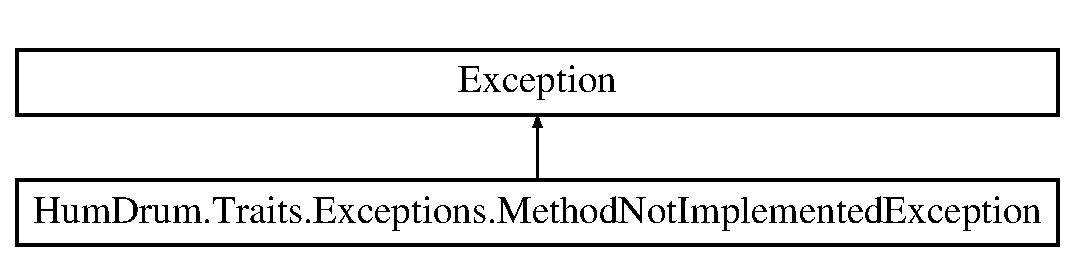
\includegraphics[height=2.000000cm]{classHumDrum_1_1Traits_1_1Exceptions_1_1MethodNotImplementedException}
\end{center}
\end{figure}
\subsection*{Public Member Functions}
\begin{DoxyCompactItemize}
\item 
\hyperlink{classHumDrum_1_1Traits_1_1Exceptions_1_1MethodNotImplementedException_a765e8aec8d09d894ee44f0d51ca626e4}{Method\+Not\+Implemented\+Exception} ()
\begin{DoxyCompactList}\small\item\em Initializes a new instance of the Hum\+Drum.\+Traits.\+Exceptions+\+Method\+Not\+Implemented\+Exception class. This will use the default message warning that a method has not been properly implemented. \end{DoxyCompactList}\item 
\hyperlink{classHumDrum_1_1Traits_1_1Exceptions_1_1MethodNotImplementedException_ad1356dbd030eda6d682496bd31d46b20}{Method\+Not\+Implemented\+Exception} (string msg)
\begin{DoxyCompactList}\small\item\em Initializes a new instance of the Hum\+Drum.\+Traits.\+Exceptions+\+Method\+Not\+Implemented\+Exception class. \end{DoxyCompactList}\item 
\hypertarget{classHumDrum_1_1Traits_1_1Exceptions_1_1MethodNotImplementedException_aadb01403cca52e9da7efacb3ff0b107c}{}{\bfseries Method\+Not\+Implemented\+Exception} (string message, Exception inner)\label{classHumDrum_1_1Traits_1_1Exceptions_1_1MethodNotImplementedException_aadb01403cca52e9da7efacb3ff0b107c}

\end{DoxyCompactItemize}


\subsection{Detailed Description}
Represents the lack of implementation of a \hyperlink{classHumDrum_1_1Traits_1_1Method}{Method} that an \hyperlink{classHumDrum_1_1Traits_1_1Interface}{Interface} specifies 



Definition at line 85 of file Exceptions.\+cs.



\subsection{Constructor \& Destructor Documentation}
\hypertarget{classHumDrum_1_1Traits_1_1Exceptions_1_1MethodNotImplementedException_a765e8aec8d09d894ee44f0d51ca626e4}{}\index{Hum\+Drum\+::\+Traits\+::\+Exceptions\+::\+Method\+Not\+Implemented\+Exception@{Hum\+Drum\+::\+Traits\+::\+Exceptions\+::\+Method\+Not\+Implemented\+Exception}!Method\+Not\+Implemented\+Exception@{Method\+Not\+Implemented\+Exception}}
\index{Method\+Not\+Implemented\+Exception@{Method\+Not\+Implemented\+Exception}!Hum\+Drum\+::\+Traits\+::\+Exceptions\+::\+Method\+Not\+Implemented\+Exception@{Hum\+Drum\+::\+Traits\+::\+Exceptions\+::\+Method\+Not\+Implemented\+Exception}}
\subsubsection[{Method\+Not\+Implemented\+Exception()}]{\setlength{\rightskip}{0pt plus 5cm}Hum\+Drum.\+Traits.\+Exceptions.\+Method\+Not\+Implemented\+Exception.\+Method\+Not\+Implemented\+Exception (
\begin{DoxyParamCaption}
{}
\end{DoxyParamCaption}
)\hspace{0.3cm}{\ttfamily [inline]}}\label{classHumDrum_1_1Traits_1_1Exceptions_1_1MethodNotImplementedException_a765e8aec8d09d894ee44f0d51ca626e4}


Initializes a new instance of the Hum\+Drum.\+Traits.\+Exceptions+\+Method\+Not\+Implemented\+Exception class. This will use the default message warning that a method has not been properly implemented. 



Definition at line 91 of file Exceptions.\+cs.

\hypertarget{classHumDrum_1_1Traits_1_1Exceptions_1_1MethodNotImplementedException_ad1356dbd030eda6d682496bd31d46b20}{}\index{Hum\+Drum\+::\+Traits\+::\+Exceptions\+::\+Method\+Not\+Implemented\+Exception@{Hum\+Drum\+::\+Traits\+::\+Exceptions\+::\+Method\+Not\+Implemented\+Exception}!Method\+Not\+Implemented\+Exception@{Method\+Not\+Implemented\+Exception}}
\index{Method\+Not\+Implemented\+Exception@{Method\+Not\+Implemented\+Exception}!Hum\+Drum\+::\+Traits\+::\+Exceptions\+::\+Method\+Not\+Implemented\+Exception@{Hum\+Drum\+::\+Traits\+::\+Exceptions\+::\+Method\+Not\+Implemented\+Exception}}
\subsubsection[{Method\+Not\+Implemented\+Exception(string msg)}]{\setlength{\rightskip}{0pt plus 5cm}Hum\+Drum.\+Traits.\+Exceptions.\+Method\+Not\+Implemented\+Exception.\+Method\+Not\+Implemented\+Exception (
\begin{DoxyParamCaption}
\item[{string}]{msg}
\end{DoxyParamCaption}
)\hspace{0.3cm}{\ttfamily [inline]}}\label{classHumDrum_1_1Traits_1_1Exceptions_1_1MethodNotImplementedException_ad1356dbd030eda6d682496bd31d46b20}


Initializes a new instance of the Hum\+Drum.\+Traits.\+Exceptions+\+Method\+Not\+Implemented\+Exception class. 


\begin{DoxyParams}{Parameters}
{\em msg} & Message.\\
\hline
\end{DoxyParams}


Definition at line 101 of file Exceptions.\+cs.



The documentation for this class was generated from the following file\+:\begin{DoxyCompactItemize}
\item 
Hum\+Drum/\+Hum\+Drum/\+Traits/Exceptions.\+cs\end{DoxyCompactItemize}

\hypertarget{classHumDrum_1_1Operations_1_1Files_1_1NumericalWriter}{}\section{Hum\+Drum.\+Operations.\+Files.\+Numerical\+Writer Class Reference}
\label{classHumDrum_1_1Operations_1_1Files_1_1NumericalWriter}\index{Hum\+Drum.\+Operations.\+Files.\+Numerical\+Writer@{Hum\+Drum.\+Operations.\+Files.\+Numerical\+Writer}}


Numerical Writer is a Sequential\+Writer that deals with numbered files  


Inheritance diagram for Hum\+Drum.\+Operations.\+Files.\+Numerical\+Writer\+:\begin{figure}[H]
\begin{center}
\leavevmode
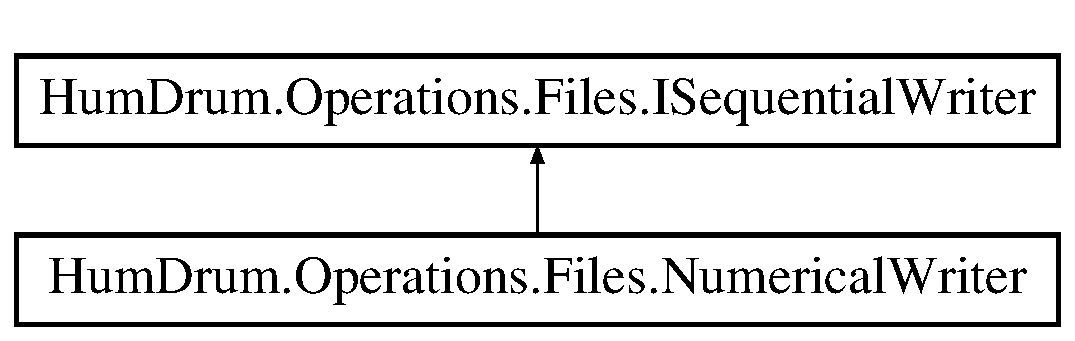
\includegraphics[height=2.000000cm]{classHumDrum_1_1Operations_1_1Files_1_1NumericalWriter}
\end{center}
\end{figure}
\subsection*{Public Member Functions}
\begin{DoxyCompactItemize}
\item 
\hyperlink{classHumDrum_1_1Operations_1_1Files_1_1NumericalWriter_a4c6486859c576a0bcf98c67688c3fd7f}{Numerical\+Writer} ()
\begin{DoxyCompactList}\small\item\em Constructor. Doesn\textquotesingle{}t have to do anything. \end{DoxyCompactList}\item 
string \hyperlink{classHumDrum_1_1Operations_1_1Files_1_1NumericalWriter_a101298a93b7984f57f8f52b802e3945e}{Name} (string directory, string extension)
\begin{DoxyCompactList}\small\item\em Attempt to find a number with the given extension that is not currently present in this directory. \end{DoxyCompactList}\item 
void \hyperlink{classHumDrum_1_1Operations_1_1Files_1_1NumericalWriter_a27becb60062cf9556fcb4063c0baf3af}{Write} (string directory, string text, string extension)
\begin{DoxyCompactList}\small\item\em Write the text to the next file in the directory \end{DoxyCompactList}\end{DoxyCompactItemize}


\subsection{Detailed Description}
Numerical Writer is a Sequential\+Writer that deals with numbered files 



Definition at line 11 of file Numerical\+Writer.\+cs.



\subsection{Constructor \& Destructor Documentation}
\hypertarget{classHumDrum_1_1Operations_1_1Files_1_1NumericalWriter_a4c6486859c576a0bcf98c67688c3fd7f}{}\index{Hum\+Drum\+::\+Operations\+::\+Files\+::\+Numerical\+Writer@{Hum\+Drum\+::\+Operations\+::\+Files\+::\+Numerical\+Writer}!Numerical\+Writer@{Numerical\+Writer}}
\index{Numerical\+Writer@{Numerical\+Writer}!Hum\+Drum\+::\+Operations\+::\+Files\+::\+Numerical\+Writer@{Hum\+Drum\+::\+Operations\+::\+Files\+::\+Numerical\+Writer}}
\subsubsection[{Numerical\+Writer()}]{\setlength{\rightskip}{0pt plus 5cm}Hum\+Drum.\+Operations.\+Files.\+Numerical\+Writer.\+Numerical\+Writer (
\begin{DoxyParamCaption}
{}
\end{DoxyParamCaption}
)\hspace{0.3cm}{\ttfamily [inline]}}\label{classHumDrum_1_1Operations_1_1Files_1_1NumericalWriter_a4c6486859c576a0bcf98c67688c3fd7f}


Constructor. Doesn\textquotesingle{}t have to do anything. 



Definition at line 16 of file Numerical\+Writer.\+cs.



\subsection{Member Function Documentation}
\hypertarget{classHumDrum_1_1Operations_1_1Files_1_1NumericalWriter_a101298a93b7984f57f8f52b802e3945e}{}\index{Hum\+Drum\+::\+Operations\+::\+Files\+::\+Numerical\+Writer@{Hum\+Drum\+::\+Operations\+::\+Files\+::\+Numerical\+Writer}!Name@{Name}}
\index{Name@{Name}!Hum\+Drum\+::\+Operations\+::\+Files\+::\+Numerical\+Writer@{Hum\+Drum\+::\+Operations\+::\+Files\+::\+Numerical\+Writer}}
\subsubsection[{Name(string directory, string extension)}]{\setlength{\rightskip}{0pt plus 5cm}string Hum\+Drum.\+Operations.\+Files.\+Numerical\+Writer.\+Name (
\begin{DoxyParamCaption}
\item[{string}]{directory, }
\item[{string}]{extension}
\end{DoxyParamCaption}
)\hspace{0.3cm}{\ttfamily [inline]}}\label{classHumDrum_1_1Operations_1_1Files_1_1NumericalWriter_a101298a93b7984f57f8f52b802e3945e}


Attempt to find a number with the given extension that is not currently present in this directory. 


\begin{DoxyParams}{Parameters}
{\em directory} & The directory to analyze\\
\hline
{\em extension} & The extension\\
\hline
\end{DoxyParams}


Implements \hyperlink{interfaceHumDrum_1_1Operations_1_1Files_1_1ISequentialWriter_aa8afc6673f6dfcc48a30732f2a6d7fa9}{Hum\+Drum.\+Operations.\+Files.\+I\+Sequential\+Writer}.



Definition at line 26 of file Numerical\+Writer.\+cs.

\hypertarget{classHumDrum_1_1Operations_1_1Files_1_1NumericalWriter_a27becb60062cf9556fcb4063c0baf3af}{}\index{Hum\+Drum\+::\+Operations\+::\+Files\+::\+Numerical\+Writer@{Hum\+Drum\+::\+Operations\+::\+Files\+::\+Numerical\+Writer}!Write@{Write}}
\index{Write@{Write}!Hum\+Drum\+::\+Operations\+::\+Files\+::\+Numerical\+Writer@{Hum\+Drum\+::\+Operations\+::\+Files\+::\+Numerical\+Writer}}
\subsubsection[{Write(string directory, string text, string extension)}]{\setlength{\rightskip}{0pt plus 5cm}void Hum\+Drum.\+Operations.\+Files.\+Numerical\+Writer.\+Write (
\begin{DoxyParamCaption}
\item[{string}]{directory, }
\item[{string}]{text, }
\item[{string}]{extension}
\end{DoxyParamCaption}
)\hspace{0.3cm}{\ttfamily [inline]}}\label{classHumDrum_1_1Operations_1_1Files_1_1NumericalWriter_a27becb60062cf9556fcb4063c0baf3af}


Write the text to the next file in the directory 


\begin{DoxyParams}{Parameters}
{\em directory} & The directory to write in\\
\hline
{\em text} & The text to write\\
\hline
{\em extension} & Extension.\\
\hline
\end{DoxyParams}


Implements \hyperlink{interfaceHumDrum_1_1Operations_1_1Files_1_1ISequentialWriter_ab9c1a57dd13d995dd5fdc35103071183}{Hum\+Drum.\+Operations.\+Files.\+I\+Sequential\+Writer}.



Definition at line 43 of file Numerical\+Writer.\+cs.



The documentation for this class was generated from the following file\+:\begin{DoxyCompactItemize}
\item 
Hum\+Drum/\+Hum\+Drum/\+Operations/\+Files/Numerical\+Writer.\+cs\end{DoxyCompactItemize}

\hypertarget{classHumDrumTests_1_1Collections_1_1Predicates}{}\section{Hum\+Drum\+Tests.\+Collections.\+Predicates Class Reference}
\label{classHumDrumTests_1_1Collections_1_1Predicates}\index{Hum\+Drum\+Tests.\+Collections.\+Predicates@{Hum\+Drum\+Tests.\+Collections.\+Predicates}}


Tests the \hyperlink{classHumDrumTests_1_1Collections_1_1Predicates}{Predicates} library in \hyperlink{namespaceHumDrum_1_1Collections}{Hum\+Drum.\+Collections}  


\subsection*{Public Member Functions}
\begin{DoxyCompactItemize}
\item 
void \hyperlink{classHumDrumTests_1_1Collections_1_1Predicates_a80acbc3096ffc25d141eceb13442f22c}{Setup} ()
\begin{DoxyCompactList}\small\item\em Sets up the variables used for testing. \end{DoxyCompactList}\item 
void \hyperlink{classHumDrumTests_1_1Collections_1_1Predicates_a3f3844173c781245d392563cf47fe74a}{Test\+Any} ()
\begin{DoxyCompactList}\small\item\em Tests both versions of the Any function \end{DoxyCompactList}\item 
void \hyperlink{classHumDrumTests_1_1Collections_1_1Predicates_adb5698404a779c6e2dbcc2e1504a7fe8}{Test\+All} ()
\begin{DoxyCompactList}\small\item\em Tests both versions of the All function \end{DoxyCompactList}\item 
void \hyperlink{classHumDrumTests_1_1Collections_1_1Predicates_afa0da270cfbb7fec7579d6744eb07bac}{Test\+Predicate\+Generators} ()
\begin{DoxyCompactList}\small\item\em Tests the predicate generators. Currently the only generators in \hyperlink{classHumDrumTests_1_1Collections_1_1Predicates}{Predicates} are for judging equality or membership. \end{DoxyCompactList}\item 
void \hyperlink{classHumDrumTests_1_1Collections_1_1Predicates_aa1910e9bf3d64229dcfe5e3dfbd54fff}{Test\+Constants} ()
\begin{DoxyCompactList}\small\item\em This tests the two predicate constants, Tautology and Contradiction \end{DoxyCompactList}\end{DoxyCompactItemize}


\subsection{Detailed Description}
Tests the \hyperlink{classHumDrumTests_1_1Collections_1_1Predicates}{Predicates} library in \hyperlink{namespaceHumDrum_1_1Collections}{Hum\+Drum.\+Collections} 



Definition at line 16 of file Predicates.\+cs.



\subsection{Member Function Documentation}
\hypertarget{classHumDrumTests_1_1Collections_1_1Predicates_a80acbc3096ffc25d141eceb13442f22c}{}\index{Hum\+Drum\+Tests\+::\+Collections\+::\+Predicates@{Hum\+Drum\+Tests\+::\+Collections\+::\+Predicates}!Setup@{Setup}}
\index{Setup@{Setup}!Hum\+Drum\+Tests\+::\+Collections\+::\+Predicates@{Hum\+Drum\+Tests\+::\+Collections\+::\+Predicates}}
\subsubsection[{Setup()}]{\setlength{\rightskip}{0pt plus 5cm}void Hum\+Drum\+Tests.\+Collections.\+Predicates.\+Setup (
\begin{DoxyParamCaption}
{}
\end{DoxyParamCaption}
)\hspace{0.3cm}{\ttfamily [inline]}}\label{classHumDrumTests_1_1Collections_1_1Predicates_a80acbc3096ffc25d141eceb13442f22c}


Sets up the variables used for testing. 



Definition at line 27 of file Predicates.\+cs.

\hypertarget{classHumDrumTests_1_1Collections_1_1Predicates_adb5698404a779c6e2dbcc2e1504a7fe8}{}\index{Hum\+Drum\+Tests\+::\+Collections\+::\+Predicates@{Hum\+Drum\+Tests\+::\+Collections\+::\+Predicates}!Test\+All@{Test\+All}}
\index{Test\+All@{Test\+All}!Hum\+Drum\+Tests\+::\+Collections\+::\+Predicates@{Hum\+Drum\+Tests\+::\+Collections\+::\+Predicates}}
\subsubsection[{Test\+All()}]{\setlength{\rightskip}{0pt plus 5cm}void Hum\+Drum\+Tests.\+Collections.\+Predicates.\+Test\+All (
\begin{DoxyParamCaption}
{}
\end{DoxyParamCaption}
)\hspace{0.3cm}{\ttfamily [inline]}}\label{classHumDrumTests_1_1Collections_1_1Predicates_adb5698404a779c6e2dbcc2e1504a7fe8}


Tests both versions of the All function 



Definition at line 62 of file Predicates.\+cs.

\hypertarget{classHumDrumTests_1_1Collections_1_1Predicates_a3f3844173c781245d392563cf47fe74a}{}\index{Hum\+Drum\+Tests\+::\+Collections\+::\+Predicates@{Hum\+Drum\+Tests\+::\+Collections\+::\+Predicates}!Test\+Any@{Test\+Any}}
\index{Test\+Any@{Test\+Any}!Hum\+Drum\+Tests\+::\+Collections\+::\+Predicates@{Hum\+Drum\+Tests\+::\+Collections\+::\+Predicates}}
\subsubsection[{Test\+Any()}]{\setlength{\rightskip}{0pt plus 5cm}void Hum\+Drum\+Tests.\+Collections.\+Predicates.\+Test\+Any (
\begin{DoxyParamCaption}
{}
\end{DoxyParamCaption}
)\hspace{0.3cm}{\ttfamily [inline]}}\label{classHumDrumTests_1_1Collections_1_1Predicates_a3f3844173c781245d392563cf47fe74a}


Tests both versions of the Any function 



Definition at line 39 of file Predicates.\+cs.

\hypertarget{classHumDrumTests_1_1Collections_1_1Predicates_aa1910e9bf3d64229dcfe5e3dfbd54fff}{}\index{Hum\+Drum\+Tests\+::\+Collections\+::\+Predicates@{Hum\+Drum\+Tests\+::\+Collections\+::\+Predicates}!Test\+Constants@{Test\+Constants}}
\index{Test\+Constants@{Test\+Constants}!Hum\+Drum\+Tests\+::\+Collections\+::\+Predicates@{Hum\+Drum\+Tests\+::\+Collections\+::\+Predicates}}
\subsubsection[{Test\+Constants()}]{\setlength{\rightskip}{0pt plus 5cm}void Hum\+Drum\+Tests.\+Collections.\+Predicates.\+Test\+Constants (
\begin{DoxyParamCaption}
{}
\end{DoxyParamCaption}
)\hspace{0.3cm}{\ttfamily [inline]}}\label{classHumDrumTests_1_1Collections_1_1Predicates_aa1910e9bf3d64229dcfe5e3dfbd54fff}


This tests the two predicate constants, Tautology and Contradiction 



Definition at line 107 of file Predicates.\+cs.

\hypertarget{classHumDrumTests_1_1Collections_1_1Predicates_afa0da270cfbb7fec7579d6744eb07bac}{}\index{Hum\+Drum\+Tests\+::\+Collections\+::\+Predicates@{Hum\+Drum\+Tests\+::\+Collections\+::\+Predicates}!Test\+Predicate\+Generators@{Test\+Predicate\+Generators}}
\index{Test\+Predicate\+Generators@{Test\+Predicate\+Generators}!Hum\+Drum\+Tests\+::\+Collections\+::\+Predicates@{Hum\+Drum\+Tests\+::\+Collections\+::\+Predicates}}
\subsubsection[{Test\+Predicate\+Generators()}]{\setlength{\rightskip}{0pt plus 5cm}void Hum\+Drum\+Tests.\+Collections.\+Predicates.\+Test\+Predicate\+Generators (
\begin{DoxyParamCaption}
{}
\end{DoxyParamCaption}
)\hspace{0.3cm}{\ttfamily [inline]}}\label{classHumDrumTests_1_1Collections_1_1Predicates_afa0da270cfbb7fec7579d6744eb07bac}


Tests the predicate generators. Currently the only generators in \hyperlink{classHumDrumTests_1_1Collections_1_1Predicates}{Predicates} are for judging equality or membership. 



Definition at line 89 of file Predicates.\+cs.



The documentation for this class was generated from the following file\+:\begin{DoxyCompactItemize}
\item 
Hum\+Drum\+Tests/\+Collections/Predicates.\+cs\end{DoxyCompactItemize}

\hypertarget{classHumDrumTests_1_1Collections_1_1Sections}{}\section{Hum\+Drum\+Tests.\+Collections.\+Sections Class Reference}
\label{classHumDrumTests_1_1Collections_1_1Sections}\index{Hum\+Drum\+Tests.\+Collections.\+Sections@{Hum\+Drum\+Tests.\+Collections.\+Sections}}


Unit Tests for the \hyperlink{classHumDrumTests_1_1Collections_1_1Sections}{Sections} library. The \hyperlink{classHumDrumTests_1_1Collections_1_1Sections}{Sections} library is first implemented using generics, but provides an abstraction of these for text. For testing purposes, testing just the text functions provides adequate proof that the underlying functions are working as intended.  


\subsection*{Public Member Functions}
\begin{DoxyCompactItemize}
\item 
void {\bfseries Setup} ()\hypertarget{classHumDrumTests_1_1Collections_1_1Sections_afac2da0762d02ff32dc3e97d479d995f}{}\label{classHumDrumTests_1_1Collections_1_1Sections_afac2da0762d02ff32dc3e97d479d995f}

\item 
void \hyperlink{classHumDrumTests_1_1Collections_1_1Sections_a0b572152156a1729cd41bc1e974f9af6}{Test\+Parse\+Sections} ()
\begin{DoxyCompactList}\small\item\em This function tests Parse\+Sections. \end{DoxyCompactList}\item 
void \hyperlink{classHumDrumTests_1_1Collections_1_1Sections_a5b6c58c513742ea5edbb4b64e1a4a92b}{Test\+Escape\+Split} ()
\begin{DoxyCompactList}\small\item\em Tests Escape\+Split \end{DoxyCompactList}\item 
void \hyperlink{classHumDrumTests_1_1Collections_1_1Sections_a4bb5d3ebc8a990cce9d1e9b34e7d65a0}{Test\+Internal} ()
\begin{DoxyCompactList}\small\item\em Tests the Internal function \end{DoxyCompactList}\item 
void \hyperlink{classHumDrumTests_1_1Collections_1_1Sections_a07bf3890ae5c723ca7cf9b73ce5eb1a7}{Test\+Globs} ()
\begin{DoxyCompactList}\small\item\em Tests the globs function \end{DoxyCompactList}\end{DoxyCompactItemize}


\subsection{Detailed Description}
Unit Tests for the \hyperlink{classHumDrumTests_1_1Collections_1_1Sections}{Sections} library. The \hyperlink{classHumDrumTests_1_1Collections_1_1Sections}{Sections} library is first implemented using generics, but provides an abstraction of these for text. For testing purposes, testing just the text functions provides adequate proof that the underlying functions are working as intended. 



Definition at line 18 of file Sections.\+cs.



\subsection{Member Function Documentation}
\index{Hum\+Drum\+Tests\+::\+Collections\+::\+Sections@{Hum\+Drum\+Tests\+::\+Collections\+::\+Sections}!Test\+Escape\+Split@{Test\+Escape\+Split}}
\index{Test\+Escape\+Split@{Test\+Escape\+Split}!Hum\+Drum\+Tests\+::\+Collections\+::\+Sections@{Hum\+Drum\+Tests\+::\+Collections\+::\+Sections}}
\subsubsection[{\texorpdfstring{Test\+Escape\+Split()}{TestEscapeSplit()}}]{\setlength{\rightskip}{0pt plus 5cm}void Hum\+Drum\+Tests.\+Collections.\+Sections.\+Test\+Escape\+Split (
\begin{DoxyParamCaption}
{}
\end{DoxyParamCaption}
)\hspace{0.3cm}{\ttfamily [inline]}}\hypertarget{classHumDrumTests_1_1Collections_1_1Sections_a5b6c58c513742ea5edbb4b64e1a4a92b}{}\label{classHumDrumTests_1_1Collections_1_1Sections_a5b6c58c513742ea5edbb4b64e1a4a92b}


Tests Escape\+Split 



Definition at line 53 of file Sections.\+cs.

\index{Hum\+Drum\+Tests\+::\+Collections\+::\+Sections@{Hum\+Drum\+Tests\+::\+Collections\+::\+Sections}!Test\+Globs@{Test\+Globs}}
\index{Test\+Globs@{Test\+Globs}!Hum\+Drum\+Tests\+::\+Collections\+::\+Sections@{Hum\+Drum\+Tests\+::\+Collections\+::\+Sections}}
\subsubsection[{\texorpdfstring{Test\+Globs()}{TestGlobs()}}]{\setlength{\rightskip}{0pt plus 5cm}void Hum\+Drum\+Tests.\+Collections.\+Sections.\+Test\+Globs (
\begin{DoxyParamCaption}
{}
\end{DoxyParamCaption}
)\hspace{0.3cm}{\ttfamily [inline]}}\hypertarget{classHumDrumTests_1_1Collections_1_1Sections_a07bf3890ae5c723ca7cf9b73ce5eb1a7}{}\label{classHumDrumTests_1_1Collections_1_1Sections_a07bf3890ae5c723ca7cf9b73ce5eb1a7}


Tests the globs function 



Definition at line 75 of file Sections.\+cs.

\index{Hum\+Drum\+Tests\+::\+Collections\+::\+Sections@{Hum\+Drum\+Tests\+::\+Collections\+::\+Sections}!Test\+Internal@{Test\+Internal}}
\index{Test\+Internal@{Test\+Internal}!Hum\+Drum\+Tests\+::\+Collections\+::\+Sections@{Hum\+Drum\+Tests\+::\+Collections\+::\+Sections}}
\subsubsection[{\texorpdfstring{Test\+Internal()}{TestInternal()}}]{\setlength{\rightskip}{0pt plus 5cm}void Hum\+Drum\+Tests.\+Collections.\+Sections.\+Test\+Internal (
\begin{DoxyParamCaption}
{}
\end{DoxyParamCaption}
)\hspace{0.3cm}{\ttfamily [inline]}}\hypertarget{classHumDrumTests_1_1Collections_1_1Sections_a4bb5d3ebc8a990cce9d1e9b34e7d65a0}{}\label{classHumDrumTests_1_1Collections_1_1Sections_a4bb5d3ebc8a990cce9d1e9b34e7d65a0}


Tests the Internal function 



Definition at line 64 of file Sections.\+cs.

\index{Hum\+Drum\+Tests\+::\+Collections\+::\+Sections@{Hum\+Drum\+Tests\+::\+Collections\+::\+Sections}!Test\+Parse\+Sections@{Test\+Parse\+Sections}}
\index{Test\+Parse\+Sections@{Test\+Parse\+Sections}!Hum\+Drum\+Tests\+::\+Collections\+::\+Sections@{Hum\+Drum\+Tests\+::\+Collections\+::\+Sections}}
\subsubsection[{\texorpdfstring{Test\+Parse\+Sections()}{TestParseSections()}}]{\setlength{\rightskip}{0pt plus 5cm}void Hum\+Drum\+Tests.\+Collections.\+Sections.\+Test\+Parse\+Sections (
\begin{DoxyParamCaption}
{}
\end{DoxyParamCaption}
)\hspace{0.3cm}{\ttfamily [inline]}}\hypertarget{classHumDrumTests_1_1Collections_1_1Sections_a0b572152156a1729cd41bc1e974f9af6}{}\label{classHumDrumTests_1_1Collections_1_1Sections_a0b572152156a1729cd41bc1e974f9af6}


This function tests Parse\+Sections. 



Definition at line 41 of file Sections.\+cs.



The documentation for this class was generated from the following file\+:\begin{DoxyCompactItemize}
\item 
Hum\+Drum\+Tests/\+Collections/Sections.\+cs\end{DoxyCompactItemize}

\hypertarget{classHumDrum_1_1Operations_1_1Servitor}{}\section{Hum\+Drum.\+Operations.\+Servitor Class Reference}
\label{classHumDrum_1_1Operations_1_1Servitor}\index{Hum\+Drum.\+Operations.\+Servitor@{Hum\+Drum.\+Operations.\+Servitor}}


\hyperlink{classHumDrum_1_1Operations_1_1Servitor}{Servitor} is a wrapper of Tcp\+Listener. It buffers incoming requests so that another thread can read them when they\textquotesingle{}d ready.  


\subsection*{Public Member Functions}
\begin{DoxyCompactItemize}
\item 
\hyperlink{classHumDrum_1_1Operations_1_1Servitor_a3da58c881e82de9be18014a186e115f5}{Servitor} ()
\begin{DoxyCompactList}\small\item\em Set up the servitor with the default settings. \end{DoxyCompactList}\item 
\hyperlink{classHumDrum_1_1Operations_1_1Servitor_ac77fd091ee638a61e42fa013c7a330ff}{Servitor} (I\+P\+Address address, int port)
\begin{DoxyCompactList}\small\item\em Create a new servitor given an I\+P\+Adress and a port. \end{DoxyCompactList}\item 
\hyperlink{classHumDrum_1_1Operations_1_1Servitor_aed529778829ebe0befe5da40f403470c}{Servitor} (I\+P\+Address address, int port, \hyperlink{classHumDrum_1_1Structures_1_1BindingsTable}{Bindings\+Table}$<$ string, string $>$ table)
\begin{DoxyCompactList}\small\item\em Initializes a new instance of the \hyperlink{classHumDrum_1_1Operations_1_1Servitor}{Hum\+Drum.\+Operations.\+Servitor} class. This allows the creation of a \hyperlink{classHumDrum_1_1Operations_1_1Servitor}{Servitor} instance with an I\+O\+Table \end{DoxyCompactList}\item 
I\+Enumerable$<$ string $>$ \hyperlink{classHumDrum_1_1Operations_1_1Servitor_af199facc3fcd3b231a75864e2c0c974b}{Collect} ()
\begin{DoxyCompactList}\small\item\em Gets all the input that the servitor has received since the last time it got any. \end{DoxyCompactList}\item 
void \hyperlink{classHumDrum_1_1Operations_1_1Servitor_a6b5653f2dc424b576a6cfdf9bfe3f021}{Start} ()
\begin{DoxyCompactList}\small\item\em Start the \hyperlink{classHumDrum_1_1Operations_1_1Servitor}{Servitor}, listening on its thread. \end{DoxyCompactList}\end{DoxyCompactItemize}
\subsection*{Static Public Member Functions}
\begin{DoxyCompactItemize}
\item 
static void \hyperlink{classHumDrum_1_1Operations_1_1Servitor_a2e2fe524ce089bcd5f0f481ff3315c40}{Send} (string data, string host, int port)
\begin{DoxyCompactList}\small\item\em Sends the specified data to the port at address \end{DoxyCompactList}\end{DoxyCompactItemize}
\subsection*{Public Attributes}
\begin{DoxyCompactItemize}
\item 
const int \hyperlink{classHumDrum_1_1Operations_1_1Servitor_a97c78f85fb9cc1c96c61ea771cc97201}{D\+E\+F\+A\+U\+L\+T\+\_\+\+P\+O\+R\+T} = 4206
\begin{DoxyCompactList}\small\item\em The default port to that \hyperlink{classHumDrum_1_1Operations_1_1Servitor}{Servitor} listens to \end{DoxyCompactList}\end{DoxyCompactItemize}
\subsection*{Properties}
\begin{DoxyCompactItemize}
\item 
bool \hyperlink{classHumDrum_1_1Operations_1_1Servitor_aacd5394a7844c38e5d4bfd96b00deefe}{Changed}\hspace{0.3cm}{\ttfamily  \mbox{[}get, set\mbox{]}}
\begin{DoxyCompactList}\small\item\em A boolean set up to determine whether input has been given since the last time it has been collected. \end{DoxyCompactList}\item 
\hyperlink{classHumDrum_1_1Structures_1_1BindingsTable}{Bindings\+Table}$<$ string, string $>$ \hyperlink{classHumDrum_1_1Operations_1_1Servitor_a01c71b67a5ca6154fd1938106b17ebf5}{I\+O\+Table}\hspace{0.3cm}{\ttfamily  \mbox{[}get, set\mbox{]}}
\begin{DoxyCompactList}\small\item\em Gets or sets the I\+O table. The I\+O Table determines, given an input, what to send to the server. \end{DoxyCompactList}\end{DoxyCompactItemize}


\subsection{Detailed Description}
\hyperlink{classHumDrum_1_1Operations_1_1Servitor}{Servitor} is a wrapper of Tcp\+Listener. It buffers incoming requests so that another thread can read them when they\textquotesingle{}d ready. 



Definition at line 17 of file Servitor.\+cs.



\subsection{Constructor \& Destructor Documentation}
\hypertarget{classHumDrum_1_1Operations_1_1Servitor_a3da58c881e82de9be18014a186e115f5}{}\index{Hum\+Drum\+::\+Operations\+::\+Servitor@{Hum\+Drum\+::\+Operations\+::\+Servitor}!Servitor@{Servitor}}
\index{Servitor@{Servitor}!Hum\+Drum\+::\+Operations\+::\+Servitor@{Hum\+Drum\+::\+Operations\+::\+Servitor}}
\subsubsection[{Servitor()}]{\setlength{\rightskip}{0pt plus 5cm}Hum\+Drum.\+Operations.\+Servitor.\+Servitor (
\begin{DoxyParamCaption}
{}
\end{DoxyParamCaption}
)\hspace{0.3cm}{\ttfamily [inline]}}\label{classHumDrum_1_1Operations_1_1Servitor_a3da58c881e82de9be18014a186e115f5}


Set up the servitor with the default settings. 



Definition at line 60 of file Servitor.\+cs.

\hypertarget{classHumDrum_1_1Operations_1_1Servitor_ac77fd091ee638a61e42fa013c7a330ff}{}\index{Hum\+Drum\+::\+Operations\+::\+Servitor@{Hum\+Drum\+::\+Operations\+::\+Servitor}!Servitor@{Servitor}}
\index{Servitor@{Servitor}!Hum\+Drum\+::\+Operations\+::\+Servitor@{Hum\+Drum\+::\+Operations\+::\+Servitor}}
\subsubsection[{Servitor(\+I\+P\+Address address, int port)}]{\setlength{\rightskip}{0pt plus 5cm}Hum\+Drum.\+Operations.\+Servitor.\+Servitor (
\begin{DoxyParamCaption}
\item[{I\+P\+Address}]{address, }
\item[{int}]{port}
\end{DoxyParamCaption}
)\hspace{0.3cm}{\ttfamily [inline]}}\label{classHumDrum_1_1Operations_1_1Servitor_ac77fd091ee638a61e42fa013c7a330ff}


Create a new servitor given an I\+P\+Adress and a port. 


\begin{DoxyParams}{Parameters}
{\em address} & The I\+P address to listen to\\
\hline
{\em port} & The port to listen on\\
\hline
\end{DoxyParams}


Definition at line 75 of file Servitor.\+cs.

\hypertarget{classHumDrum_1_1Operations_1_1Servitor_aed529778829ebe0befe5da40f403470c}{}\index{Hum\+Drum\+::\+Operations\+::\+Servitor@{Hum\+Drum\+::\+Operations\+::\+Servitor}!Servitor@{Servitor}}
\index{Servitor@{Servitor}!Hum\+Drum\+::\+Operations\+::\+Servitor@{Hum\+Drum\+::\+Operations\+::\+Servitor}}
\subsubsection[{Servitor(\+I\+P\+Address address, int port, Bindings\+Table$<$ string, string $>$ table)}]{\setlength{\rightskip}{0pt plus 5cm}Hum\+Drum.\+Operations.\+Servitor.\+Servitor (
\begin{DoxyParamCaption}
\item[{I\+P\+Address}]{address, }
\item[{int}]{port, }
\item[{{\bf Bindings\+Table}$<$ string, string $>$}]{table}
\end{DoxyParamCaption}
)\hspace{0.3cm}{\ttfamily [inline]}}\label{classHumDrum_1_1Operations_1_1Servitor_aed529778829ebe0befe5da40f403470c}


Initializes a new instance of the \hyperlink{classHumDrum_1_1Operations_1_1Servitor}{Hum\+Drum.\+Operations.\+Servitor} class. This allows the creation of a \hyperlink{classHumDrum_1_1Operations_1_1Servitor}{Servitor} instance with an I\+O\+Table 


\begin{DoxyParams}{Parameters}
{\em address} & The address to listen to\\
\hline
{\em port} & The port to listen to\\
\hline
{\em table} & The table of inputs and outputs\\
\hline
\end{DoxyParams}


Definition at line 90 of file Servitor.\+cs.



\subsection{Member Function Documentation}
\hypertarget{classHumDrum_1_1Operations_1_1Servitor_af199facc3fcd3b231a75864e2c0c974b}{}\index{Hum\+Drum\+::\+Operations\+::\+Servitor@{Hum\+Drum\+::\+Operations\+::\+Servitor}!Collect@{Collect}}
\index{Collect@{Collect}!Hum\+Drum\+::\+Operations\+::\+Servitor@{Hum\+Drum\+::\+Operations\+::\+Servitor}}
\subsubsection[{Collect()}]{\setlength{\rightskip}{0pt plus 5cm}I\+Enumerable$<$string$>$ Hum\+Drum.\+Operations.\+Servitor.\+Collect (
\begin{DoxyParamCaption}
{}
\end{DoxyParamCaption}
)\hspace{0.3cm}{\ttfamily [inline]}}\label{classHumDrum_1_1Operations_1_1Servitor_af199facc3fcd3b231a75864e2c0c974b}


Gets all the input that the servitor has received since the last time it got any. 

\begin{DoxyReturn}{Returns}
The list of the new input
\end{DoxyReturn}


Definition at line 100 of file Servitor.\+cs.

\hypertarget{classHumDrum_1_1Operations_1_1Servitor_a2e2fe524ce089bcd5f0f481ff3315c40}{}\index{Hum\+Drum\+::\+Operations\+::\+Servitor@{Hum\+Drum\+::\+Operations\+::\+Servitor}!Send@{Send}}
\index{Send@{Send}!Hum\+Drum\+::\+Operations\+::\+Servitor@{Hum\+Drum\+::\+Operations\+::\+Servitor}}
\subsubsection[{Send(string data, string host, int port)}]{\setlength{\rightskip}{0pt plus 5cm}static void Hum\+Drum.\+Operations.\+Servitor.\+Send (
\begin{DoxyParamCaption}
\item[{string}]{data, }
\item[{string}]{host, }
\item[{int}]{port}
\end{DoxyParamCaption}
)\hspace{0.3cm}{\ttfamily [inline]}, {\ttfamily [static]}}\label{classHumDrum_1_1Operations_1_1Servitor_a2e2fe524ce089bcd5f0f481ff3315c40}


Sends the specified data to the port at address 


\begin{DoxyParams}{Parameters}
{\em data} & The data to send as a string\\
\hline
{\em address} & The address to send the data to\\
\hline
{\em port} & The port to which the data should be sent\\
\hline
\end{DoxyParams}


Definition at line 168 of file Servitor.\+cs.

\hypertarget{classHumDrum_1_1Operations_1_1Servitor_a6b5653f2dc424b576a6cfdf9bfe3f021}{}\index{Hum\+Drum\+::\+Operations\+::\+Servitor@{Hum\+Drum\+::\+Operations\+::\+Servitor}!Start@{Start}}
\index{Start@{Start}!Hum\+Drum\+::\+Operations\+::\+Servitor@{Hum\+Drum\+::\+Operations\+::\+Servitor}}
\subsubsection[{Start()}]{\setlength{\rightskip}{0pt plus 5cm}void Hum\+Drum.\+Operations.\+Servitor.\+Start (
\begin{DoxyParamCaption}
{}
\end{DoxyParamCaption}
)\hspace{0.3cm}{\ttfamily [inline]}}\label{classHumDrum_1_1Operations_1_1Servitor_a6b5653f2dc424b576a6cfdf9bfe3f021}


Start the \hyperlink{classHumDrum_1_1Operations_1_1Servitor}{Servitor}, listening on its thread. 



Definition at line 119 of file Servitor.\+cs.



\subsection{Member Data Documentation}
\hypertarget{classHumDrum_1_1Operations_1_1Servitor_a97c78f85fb9cc1c96c61ea771cc97201}{}\index{Hum\+Drum\+::\+Operations\+::\+Servitor@{Hum\+Drum\+::\+Operations\+::\+Servitor}!D\+E\+F\+A\+U\+L\+T\+\_\+\+P\+O\+R\+T@{D\+E\+F\+A\+U\+L\+T\+\_\+\+P\+O\+R\+T}}
\index{D\+E\+F\+A\+U\+L\+T\+\_\+\+P\+O\+R\+T@{D\+E\+F\+A\+U\+L\+T\+\_\+\+P\+O\+R\+T}!Hum\+Drum\+::\+Operations\+::\+Servitor@{Hum\+Drum\+::\+Operations\+::\+Servitor}}
\subsubsection[{D\+E\+F\+A\+U\+L\+T\+\_\+\+P\+O\+R\+T}]{\setlength{\rightskip}{0pt plus 5cm}const int Hum\+Drum.\+Operations.\+Servitor.\+D\+E\+F\+A\+U\+L\+T\+\_\+\+P\+O\+R\+T = 4206}\label{classHumDrum_1_1Operations_1_1Servitor_a97c78f85fb9cc1c96c61ea771cc97201}


The default port to that \hyperlink{classHumDrum_1_1Operations_1_1Servitor}{Servitor} listens to 



Definition at line 55 of file Servitor.\+cs.



\subsection{Property Documentation}
\hypertarget{classHumDrum_1_1Operations_1_1Servitor_aacd5394a7844c38e5d4bfd96b00deefe}{}\index{Hum\+Drum\+::\+Operations\+::\+Servitor@{Hum\+Drum\+::\+Operations\+::\+Servitor}!Changed@{Changed}}
\index{Changed@{Changed}!Hum\+Drum\+::\+Operations\+::\+Servitor@{Hum\+Drum\+::\+Operations\+::\+Servitor}}
\subsubsection[{Changed}]{\setlength{\rightskip}{0pt plus 5cm}bool Hum\+Drum.\+Operations.\+Servitor.\+Changed\hspace{0.3cm}{\ttfamily [get]}, {\ttfamily [set]}}\label{classHumDrum_1_1Operations_1_1Servitor_aacd5394a7844c38e5d4bfd96b00deefe}


A boolean set up to determine whether input has been given since the last time it has been collected. 



Definition at line 38 of file Servitor.\+cs.

\hypertarget{classHumDrum_1_1Operations_1_1Servitor_a01c71b67a5ca6154fd1938106b17ebf5}{}\index{Hum\+Drum\+::\+Operations\+::\+Servitor@{Hum\+Drum\+::\+Operations\+::\+Servitor}!I\+O\+Table@{I\+O\+Table}}
\index{I\+O\+Table@{I\+O\+Table}!Hum\+Drum\+::\+Operations\+::\+Servitor@{Hum\+Drum\+::\+Operations\+::\+Servitor}}
\subsubsection[{I\+O\+Table}]{\setlength{\rightskip}{0pt plus 5cm}{\bf Bindings\+Table}$<$string, string$>$ Hum\+Drum.\+Operations.\+Servitor.\+I\+O\+Table\hspace{0.3cm}{\ttfamily [get]}, {\ttfamily [set]}}\label{classHumDrum_1_1Operations_1_1Servitor_a01c71b67a5ca6154fd1938106b17ebf5}


Gets or sets the I\+O table. The I\+O Table determines, given an input, what to send to the server. 

The I\+O table

Definition at line 50 of file Servitor.\+cs.



The documentation for this class was generated from the following file\+:\begin{DoxyCompactItemize}
\item 
Hum\+Drum/\+Hum\+Drum/\+Operations/Servitor.\+cs\end{DoxyCompactItemize}

\hypertarget{classHumDrum_1_1Collections_1_1Groups_1_1StateObject}{}\section{Hum\+Drum.\+Collections.\+Groups.\+State\+Object$<$ T $>$ Class Template Reference}
\label{classHumDrum_1_1Collections_1_1Groups_1_1StateObject}\index{Hum\+Drum.\+Collections.\+Groups.\+State\+Object$<$ T $>$@{Hum\+Drum.\+Collections.\+Groups.\+State\+Object$<$ T $>$}}


The construct for the state machines. These functions set and apply the rules for checking and modifying state.  


\subsection*{Public Member Functions}
\begin{DoxyCompactItemize}
\item 
virtual bool \hyperlink{classHumDrum_1_1Collections_1_1Groups_1_1StateObject_a227e83d9109b0022d195afea296ea0fd}{Modify\+State} (T capture)
\begin{DoxyCompactList}\small\item\em Modifies the current state based on this instance\textquotesingle{}s Modifier. This method is meant to be overriden to accomodate for the captured element as an additional modification of the machine\textquotesingle{}s state. \end{DoxyCompactList}\item 
bool \hyperlink{classHumDrum_1_1Collections_1_1Groups_1_1StateObject_a633a33ef5ac78aa8686c49a626f50376}{Modify\+State} ()
\begin{DoxyCompactList}\small\item\em Modify the state using only the modifier. \end{DoxyCompactList}\item 
virtual void \hyperlink{classHumDrum_1_1Collections_1_1Groups_1_1StateObject_aecd06a8d2511a91f5b1422c8fe3836b2}{Reset} ()
\begin{DoxyCompactList}\small\item\em Function meant to be overriden by \hyperlink{namespaceHumDrum_1_1Collections_1_1StateModifiers}{State\+Modifiers} in order to reset after Groups parsing. \end{DoxyCompactList}\end{DoxyCompactItemize}
\subsection*{Properties}
\begin{DoxyCompactItemize}
\item 
T \hyperlink{classHumDrum_1_1Collections_1_1Groups_1_1StateObject_a192fdeea48e27612063d5099456ec217}{State}\hspace{0.3cm}{\ttfamily  \mbox{[}get, set\mbox{]}}
\begin{DoxyCompactList}\small\item\em Gets or sets the current state of this machine. \end{DoxyCompactList}\item 
State\+Check$<$ T $>$ \hyperlink{classHumDrum_1_1Collections_1_1Groups_1_1StateObject_aca3a9433c50c52f7364d5239d3847749}{Check}\hspace{0.3cm}{\ttfamily  \mbox{[}get, set\mbox{]}}
\begin{DoxyCompactList}\small\item\em The function used to check the state of this machine \end{DoxyCompactList}\item 
State\+Modify$<$ T $>$ \hyperlink{classHumDrum_1_1Collections_1_1Groups_1_1StateObject_a0d961b56d3c86f24a5185cb1812285ac}{Modifier}\hspace{0.3cm}{\ttfamily  \mbox{[}get, set\mbox{]}}
\begin{DoxyCompactList}\small\item\em The function used to modify the state of this machine \end{DoxyCompactList}\end{DoxyCompactItemize}


\subsection{Detailed Description}
The construct for the state machines. These functions set and apply the rules for checking and modifying state. 



Definition at line 30 of file Groups.\+cs.



\subsection{Member Function Documentation}
\hypertarget{classHumDrum_1_1Collections_1_1Groups_1_1StateObject_a227e83d9109b0022d195afea296ea0fd}{}\index{Hum\+Drum\+::\+Collections\+::\+Groups\+::\+State\+Object@{Hum\+Drum\+::\+Collections\+::\+Groups\+::\+State\+Object}!Modify\+State@{Modify\+State}}
\index{Modify\+State@{Modify\+State}!Hum\+Drum\+::\+Collections\+::\+Groups\+::\+State\+Object@{Hum\+Drum\+::\+Collections\+::\+Groups\+::\+State\+Object}}
\subsubsection[{Modify\+State(\+T capture)}]{\setlength{\rightskip}{0pt plus 5cm}virtual bool {\bf Hum\+Drum.\+Collections.\+Groups.\+State\+Object}$<$ T $>$.Modify\+State (
\begin{DoxyParamCaption}
\item[{T}]{capture}
\end{DoxyParamCaption}
)\hspace{0.3cm}{\ttfamily [inline]}, {\ttfamily [virtual]}}\label{classHumDrum_1_1Collections_1_1Groups_1_1StateObject_a227e83d9109b0022d195afea296ea0fd}


Modifies the current state based on this instance\textquotesingle{}s Modifier. This method is meant to be overriden to accomodate for the captured element as an additional modification of the machine\textquotesingle{}s state. 

\begin{DoxyReturn}{Returns}
{\ttfamily true}, if the check A\+F\+T\+E\+R modification is true$<$c$>$false otherwise.
\end{DoxyReturn}

\begin{DoxyParams}{Parameters}
{\em capture} & The item in a list\\
\hline
\end{DoxyParams}


Definition at line 59 of file Groups.\+cs.

\hypertarget{classHumDrum_1_1Collections_1_1Groups_1_1StateObject_a633a33ef5ac78aa8686c49a626f50376}{}\index{Hum\+Drum\+::\+Collections\+::\+Groups\+::\+State\+Object@{Hum\+Drum\+::\+Collections\+::\+Groups\+::\+State\+Object}!Modify\+State@{Modify\+State}}
\index{Modify\+State@{Modify\+State}!Hum\+Drum\+::\+Collections\+::\+Groups\+::\+State\+Object@{Hum\+Drum\+::\+Collections\+::\+Groups\+::\+State\+Object}}
\subsubsection[{Modify\+State()}]{\setlength{\rightskip}{0pt plus 5cm}bool {\bf Hum\+Drum.\+Collections.\+Groups.\+State\+Object}$<$ T $>$.Modify\+State (
\begin{DoxyParamCaption}
{}
\end{DoxyParamCaption}
)\hspace{0.3cm}{\ttfamily [inline]}}\label{classHumDrum_1_1Collections_1_1Groups_1_1StateObject_a633a33ef5ac78aa8686c49a626f50376}


Modify the state using only the modifier. 

\begin{DoxyReturn}{Returns}
{\ttfamily true}, if state was modifyed, {\ttfamily false} otherwise.
\end{DoxyReturn}


Definition at line 69 of file Groups.\+cs.

\hypertarget{classHumDrum_1_1Collections_1_1Groups_1_1StateObject_aecd06a8d2511a91f5b1422c8fe3836b2}{}\index{Hum\+Drum\+::\+Collections\+::\+Groups\+::\+State\+Object@{Hum\+Drum\+::\+Collections\+::\+Groups\+::\+State\+Object}!Reset@{Reset}}
\index{Reset@{Reset}!Hum\+Drum\+::\+Collections\+::\+Groups\+::\+State\+Object@{Hum\+Drum\+::\+Collections\+::\+Groups\+::\+State\+Object}}
\subsubsection[{Reset()}]{\setlength{\rightskip}{0pt plus 5cm}virtual void {\bf Hum\+Drum.\+Collections.\+Groups.\+State\+Object}$<$ T $>$.Reset (
\begin{DoxyParamCaption}
{}
\end{DoxyParamCaption}
)\hspace{0.3cm}{\ttfamily [inline]}, {\ttfamily [virtual]}}\label{classHumDrum_1_1Collections_1_1Groups_1_1StateObject_aecd06a8d2511a91f5b1422c8fe3836b2}


Function meant to be overriden by \hyperlink{namespaceHumDrum_1_1Collections_1_1StateModifiers}{State\+Modifiers} in order to reset after Groups parsing. 



Reimplemented in \hyperlink{classHumDrum_1_1Collections_1_1StateModifiers_1_1IntegerCounter_a8723ab8842f09ee98d9e13b7714d14a7}{Hum\+Drum.\+Collections.\+State\+Modifiers.\+Integer\+Counter}.



Definition at line 79 of file Groups.\+cs.



\subsection{Property Documentation}
\hypertarget{classHumDrum_1_1Collections_1_1Groups_1_1StateObject_aca3a9433c50c52f7364d5239d3847749}{}\index{Hum\+Drum\+::\+Collections\+::\+Groups\+::\+State\+Object@{Hum\+Drum\+::\+Collections\+::\+Groups\+::\+State\+Object}!Check@{Check}}
\index{Check@{Check}!Hum\+Drum\+::\+Collections\+::\+Groups\+::\+State\+Object@{Hum\+Drum\+::\+Collections\+::\+Groups\+::\+State\+Object}}
\subsubsection[{Check}]{\setlength{\rightskip}{0pt plus 5cm}State\+Check$<$T$>$ {\bf Hum\+Drum.\+Collections.\+Groups.\+State\+Object}$<$ T $>$.Check\hspace{0.3cm}{\ttfamily [get]}, {\ttfamily [set]}}\label{classHumDrum_1_1Collections_1_1Groups_1_1StateObject_aca3a9433c50c52f7364d5239d3847749}


The function used to check the state of this machine 

The predicate function

Definition at line 44 of file Groups.\+cs.

\hypertarget{classHumDrum_1_1Collections_1_1Groups_1_1StateObject_a0d961b56d3c86f24a5185cb1812285ac}{}\index{Hum\+Drum\+::\+Collections\+::\+Groups\+::\+State\+Object@{Hum\+Drum\+::\+Collections\+::\+Groups\+::\+State\+Object}!Modifier@{Modifier}}
\index{Modifier@{Modifier}!Hum\+Drum\+::\+Collections\+::\+Groups\+::\+State\+Object@{Hum\+Drum\+::\+Collections\+::\+Groups\+::\+State\+Object}}
\subsubsection[{Modifier}]{\setlength{\rightskip}{0pt plus 5cm}State\+Modify$<$T$>$ {\bf Hum\+Drum.\+Collections.\+Groups.\+State\+Object}$<$ T $>$.Modifier\hspace{0.3cm}{\ttfamily [get]}, {\ttfamily [set]}}\label{classHumDrum_1_1Collections_1_1Groups_1_1StateObject_a0d961b56d3c86f24a5185cb1812285ac}


The function used to modify the state of this machine 

The pure modifier function

Definition at line 50 of file Groups.\+cs.

\hypertarget{classHumDrum_1_1Collections_1_1Groups_1_1StateObject_a192fdeea48e27612063d5099456ec217}{}\index{Hum\+Drum\+::\+Collections\+::\+Groups\+::\+State\+Object@{Hum\+Drum\+::\+Collections\+::\+Groups\+::\+State\+Object}!State@{State}}
\index{State@{State}!Hum\+Drum\+::\+Collections\+::\+Groups\+::\+State\+Object@{Hum\+Drum\+::\+Collections\+::\+Groups\+::\+State\+Object}}
\subsubsection[{State}]{\setlength{\rightskip}{0pt plus 5cm}T {\bf Hum\+Drum.\+Collections.\+Groups.\+State\+Object}$<$ T $>$.State\hspace{0.3cm}{\ttfamily [get]}, {\ttfamily [set]}}\label{classHumDrum_1_1Collections_1_1Groups_1_1StateObject_a192fdeea48e27612063d5099456ec217}


Gets or sets the current state of this machine. 

The state

Definition at line 37 of file Groups.\+cs.



The documentation for this class was generated from the following file\+:\begin{DoxyCompactItemize}
\item 
Hum\+Drum/\+Hum\+Drum/\+Collections/Groups.\+cs\end{DoxyCompactItemize}

\hypertarget{classHumDrumTests_1_1Test}{}\section{Hum\+Drum\+Tests.\+Test Class Reference}
\label{classHumDrumTests_1_1Test}\index{Hum\+Drum\+Tests.\+Test@{Hum\+Drum\+Tests.\+Test}}
\subsection*{Public Member Functions}
\begin{DoxyCompactItemize}
\item 
void {\bfseries Test\+Case} ()\hypertarget{classHumDrumTests_1_1Test_a4beeda58524488aabd71179fd5dcf8f8}{}\label{classHumDrumTests_1_1Test_a4beeda58524488aabd71179fd5dcf8f8}

\end{DoxyCompactItemize}


\subsection{Detailed Description}


Definition at line 7 of file Test.\+cs.



The documentation for this class was generated from the following file\+:\begin{DoxyCompactItemize}
\item 
Hum\+Drum\+Tests/Test.\+cs\end{DoxyCompactItemize}

\hypertarget{classHumDrum_1_1Traits_1_1Trait}{}\section{Hum\+Drum.\+Traits.\+Trait Class Reference}
\label{classHumDrum_1_1Traits_1_1Trait}\index{Hum\+Drum.\+Traits.\+Trait@{Hum\+Drum.\+Traits.\+Trait}}


A \hyperlink{classHumDrum_1_1Traits_1_1Trait}{Trait} is a description of a class\textquotesingle{}s capabilities. This closely resembles an interface, but with one key difference -\/ interfaces must be implemented by a class within it, never after.  


\subsection*{Public Member Functions}
\begin{DoxyCompactItemize}
\item 
\hyperlink{classHumDrum_1_1Traits_1_1Trait_a190ac07fbda083c60d556d39e5463a06}{Trait} (\hyperlink{classHumDrum_1_1Traits_1_1Interface}{Interface} blueprint, \hyperlink{classHumDrum_1_1Traits_1_1Class}{Class} implementor)
\begin{DoxyCompactList}\small\item\em Initializes a new instance of the \hyperlink{classHumDrum_1_1Traits_1_1Trait}{Hum\+Drum.\+Traits.\+Trait} class. This will not test to see if \end{DoxyCompactList}\item 
\hyperlink{classHumDrum_1_1Traits_1_1Trait_ad2465a9da468106741fd2a58495e0735}{Trait} (Type the\+Interface, Type the\+Implementor)
\begin{DoxyCompactList}\small\item\em Initializes a new instance of the \hyperlink{classHumDrum_1_1Traits_1_1Trait}{Hum\+Drum.\+Traits.\+Trait} class. This uses two traits which are immediately cast to an \hyperlink{classHumDrum_1_1Traits_1_1Interface}{Interface} and \hyperlink{classHumDrum_1_1Traits_1_1Class}{Class}. \end{DoxyCompactList}\item 
void \hyperlink{classHumDrum_1_1Traits_1_1Trait_a41641af3ce5a397fd0371da282e261bf}{Add\+Method} (\hyperlink{classHumDrum_1_1Traits_1_1Method}{Method} m)
\begin{DoxyCompactList}\small\item\em Adds a \hyperlink{classHumDrum_1_1Traits_1_1Method}{Method} to the implementor class \end{DoxyCompactList}\item 
void \hyperlink{classHumDrum_1_1Traits_1_1Trait_a8f2c39015aebfa0eb31149e5c5d04645}{Add\+Method} (Type typ, string method\+Name)
\begin{DoxyCompactList}\small\item\em Adds a Type t to the Inner\+Class as a \hyperlink{classHumDrum_1_1Traits_1_1Method}{Method} \end{DoxyCompactList}\item 
void \hyperlink{classHumDrum_1_1Traits_1_1Trait_a91a98e327a4208ac39a2c610fd6d7bd9}{Add\+Method} (Method\+Info mi, string method\+Name)
\begin{DoxyCompactList}\small\item\em Adds a \hyperlink{classHumDrum_1_1Traits_1_1Method}{Method} from Method\+Info, binding it optionally with a name \end{DoxyCompactList}\item 
void \hyperlink{classHumDrum_1_1Traits_1_1Trait_a3f7d772a82dc19c402bb08ce00c4f068}{Add\+Method} (string method\+Name, Delegate d)
\begin{DoxyCompactList}\small\item\em Coerces this Delegate into a \hyperlink{classHumDrum_1_1Traits_1_1Method}{Method} and adds it to this trait \end{DoxyCompactList}\item 
bool \hyperlink{classHumDrum_1_1Traits_1_1Trait_a6a63ae3fa959009dcc166b48a7ade10a}{Is\+Satisfied} ()
\begin{DoxyCompactList}\small\item\em Tests to see whether or not the implementor satisfies the given class \end{DoxyCompactList}\item 
\hyperlink{classHumDrum_1_1Traits_1_1Method}{Method} \hyperlink{classHumDrum_1_1Traits_1_1Trait_a64761f85f3de19b1eb406a963ff4929b}{The} (string function\+Name)
\begin{DoxyCompactList}\small\item\em Gets a named \hyperlink{classHumDrum_1_1Traits_1_1Method}{Method} from the implementing class \end{DoxyCompactList}\end{DoxyCompactItemize}
\subsection*{Properties}
\begin{DoxyCompactItemize}
\item 
string \hyperlink{classHumDrum_1_1Traits_1_1Trait_a1127f27ad57f5578c010c4785eac06b3}{Name}\hspace{0.3cm}{\ttfamily  \mbox{[}get, set\mbox{]}}
\begin{DoxyCompactList}\small\item\em The name of this trait \end{DoxyCompactList}\item 
\hyperlink{classHumDrum_1_1Traits_1_1Interface}{Interface} \hyperlink{classHumDrum_1_1Traits_1_1Trait_a44f53e84d7ce34f84ce3be1e60345368}{Required\+Methods}\hspace{0.3cm}{\ttfamily  \mbox{[}get, set\mbox{]}}
\begin{DoxyCompactList}\small\item\em The \hyperlink{classHumDrum_1_1Traits_1_1Interface}{Interface} which describes \end{DoxyCompactList}\item 
\hyperlink{classHumDrum_1_1Traits_1_1Class}{Class} \hyperlink{classHumDrum_1_1Traits_1_1Trait_adcd5827803b20072ff79bb25ce03f055}{Implementing\+Class}\hspace{0.3cm}{\ttfamily  \mbox{[}get, set\mbox{]}}
\begin{DoxyCompactList}\small\item\em The class which implements the methods that the interface requires \end{DoxyCompactList}\end{DoxyCompactItemize}


\subsection{Detailed Description}
A \hyperlink{classHumDrum_1_1Traits_1_1Trait}{Trait} is a description of a class\textquotesingle{}s capabilities. This closely resembles an interface, but with one key difference -\/ interfaces must be implemented by a class within it, never after. 

\hyperlink{namespaceHumDrum_1_1Traits}{Traits} allow you to satiate the requirements of an interface separately from the class definition, which lets you describe how some class that you did not make interacts with an interface. 

Definition at line 17 of file Trait.\+cs.



\subsection{Constructor \& Destructor Documentation}
\index{Hum\+Drum\+::\+Traits\+::\+Trait@{Hum\+Drum\+::\+Traits\+::\+Trait}!Trait@{Trait}}
\index{Trait@{Trait}!Hum\+Drum\+::\+Traits\+::\+Trait@{Hum\+Drum\+::\+Traits\+::\+Trait}}
\subsubsection[{\texorpdfstring{Trait(\+Interface blueprint, Class implementor)}{Trait(Interface blueprint, Class implementor)}}]{\setlength{\rightskip}{0pt plus 5cm}Hum\+Drum.\+Traits.\+Trait.\+Trait (
\begin{DoxyParamCaption}
\item[{{\bf Interface}}]{blueprint, }
\item[{{\bf Class}}]{implementor}
\end{DoxyParamCaption}
)\hspace{0.3cm}{\ttfamily [inline]}}\hypertarget{classHumDrum_1_1Traits_1_1Trait_a190ac07fbda083c60d556d39e5463a06}{}\label{classHumDrum_1_1Traits_1_1Trait_a190ac07fbda083c60d556d39e5463a06}


Initializes a new instance of the \hyperlink{classHumDrum_1_1Traits_1_1Trait}{Hum\+Drum.\+Traits.\+Trait} class. This will not test to see if 


\begin{DoxyParams}{Parameters}
{\em blueprint} & Blueprint.\\
\hline
{\em implementor} & \hyperlink{classHumDrum_1_1Traits_1_1Implementor}{Implementor}.\\
\hline
\end{DoxyParams}


Definition at line 43 of file Trait.\+cs.

\index{Hum\+Drum\+::\+Traits\+::\+Trait@{Hum\+Drum\+::\+Traits\+::\+Trait}!Trait@{Trait}}
\index{Trait@{Trait}!Hum\+Drum\+::\+Traits\+::\+Trait@{Hum\+Drum\+::\+Traits\+::\+Trait}}
\subsubsection[{\texorpdfstring{Trait(\+Type the\+Interface, Type the\+Implementor)}{Trait(Type theInterface, Type theImplementor)}}]{\setlength{\rightskip}{0pt plus 5cm}Hum\+Drum.\+Traits.\+Trait.\+Trait (
\begin{DoxyParamCaption}
\item[{Type}]{the\+Interface, }
\item[{Type}]{the\+Implementor}
\end{DoxyParamCaption}
)\hspace{0.3cm}{\ttfamily [inline]}}\hypertarget{classHumDrum_1_1Traits_1_1Trait_ad2465a9da468106741fd2a58495e0735}{}\label{classHumDrum_1_1Traits_1_1Trait_ad2465a9da468106741fd2a58495e0735}


Initializes a new instance of the \hyperlink{classHumDrum_1_1Traits_1_1Trait}{Hum\+Drum.\+Traits.\+Trait} class. This uses two traits which are immediately cast to an \hyperlink{classHumDrum_1_1Traits_1_1Interface}{Interface} and \hyperlink{classHumDrum_1_1Traits_1_1Class}{Class}. 


\begin{DoxyParams}{Parameters}
{\em the\+Interface} & The interface\\
\hline
{\em the\+Implementor} & The implementor\\
\hline
\end{DoxyParams}


Definition at line 55 of file Trait.\+cs.



\subsection{Member Function Documentation}
\index{Hum\+Drum\+::\+Traits\+::\+Trait@{Hum\+Drum\+::\+Traits\+::\+Trait}!Add\+Method@{Add\+Method}}
\index{Add\+Method@{Add\+Method}!Hum\+Drum\+::\+Traits\+::\+Trait@{Hum\+Drum\+::\+Traits\+::\+Trait}}
\subsubsection[{\texorpdfstring{Add\+Method(\+Method m)}{AddMethod(Method m)}}]{\setlength{\rightskip}{0pt plus 5cm}void Hum\+Drum.\+Traits.\+Trait.\+Add\+Method (
\begin{DoxyParamCaption}
\item[{{\bf Method}}]{m}
\end{DoxyParamCaption}
)\hspace{0.3cm}{\ttfamily [inline]}}\hypertarget{classHumDrum_1_1Traits_1_1Trait_a41641af3ce5a397fd0371da282e261bf}{}\label{classHumDrum_1_1Traits_1_1Trait_a41641af3ce5a397fd0371da282e261bf}


Adds a \hyperlink{classHumDrum_1_1Traits_1_1Method}{Method} to the implementor class 


\begin{DoxyParams}{Parameters}
{\em m} & The method\\
\hline
\end{DoxyParams}


Definition at line 65 of file Trait.\+cs.

\index{Hum\+Drum\+::\+Traits\+::\+Trait@{Hum\+Drum\+::\+Traits\+::\+Trait}!Add\+Method@{Add\+Method}}
\index{Add\+Method@{Add\+Method}!Hum\+Drum\+::\+Traits\+::\+Trait@{Hum\+Drum\+::\+Traits\+::\+Trait}}
\subsubsection[{\texorpdfstring{Add\+Method(\+Type typ, string method\+Name)}{AddMethod(Type typ, string methodName)}}]{\setlength{\rightskip}{0pt plus 5cm}void Hum\+Drum.\+Traits.\+Trait.\+Add\+Method (
\begin{DoxyParamCaption}
\item[{Type}]{typ, }
\item[{string}]{method\+Name}
\end{DoxyParamCaption}
)\hspace{0.3cm}{\ttfamily [inline]}}\hypertarget{classHumDrum_1_1Traits_1_1Trait_a8f2c39015aebfa0eb31149e5c5d04645}{}\label{classHumDrum_1_1Traits_1_1Trait_a8f2c39015aebfa0eb31149e5c5d04645}


Adds a Type t to the Inner\+Class as a \hyperlink{classHumDrum_1_1Traits_1_1Method}{Method} 


\begin{DoxyParams}{Parameters}
{\em t} & The method to add\\
\hline
\end{DoxyParams}


Definition at line 74 of file Trait.\+cs.

\index{Hum\+Drum\+::\+Traits\+::\+Trait@{Hum\+Drum\+::\+Traits\+::\+Trait}!Add\+Method@{Add\+Method}}
\index{Add\+Method@{Add\+Method}!Hum\+Drum\+::\+Traits\+::\+Trait@{Hum\+Drum\+::\+Traits\+::\+Trait}}
\subsubsection[{\texorpdfstring{Add\+Method(\+Method\+Info mi, string method\+Name)}{AddMethod(MethodInfo mi, string methodName)}}]{\setlength{\rightskip}{0pt plus 5cm}void Hum\+Drum.\+Traits.\+Trait.\+Add\+Method (
\begin{DoxyParamCaption}
\item[{Method\+Info}]{mi, }
\item[{string}]{method\+Name}
\end{DoxyParamCaption}
)\hspace{0.3cm}{\ttfamily [inline]}}\hypertarget{classHumDrum_1_1Traits_1_1Trait_a91a98e327a4208ac39a2c610fd6d7bd9}{}\label{classHumDrum_1_1Traits_1_1Trait_a91a98e327a4208ac39a2c610fd6d7bd9}


Adds a \hyperlink{classHumDrum_1_1Traits_1_1Method}{Method} from Method\+Info, binding it optionally with a name 


\begin{DoxyParams}{Parameters}
{\em mi} & The method info\\
\hline
{\em method\+Name} & The name of the method\\
\hline
\end{DoxyParams}


Definition at line 84 of file Trait.\+cs.

\index{Hum\+Drum\+::\+Traits\+::\+Trait@{Hum\+Drum\+::\+Traits\+::\+Trait}!Add\+Method@{Add\+Method}}
\index{Add\+Method@{Add\+Method}!Hum\+Drum\+::\+Traits\+::\+Trait@{Hum\+Drum\+::\+Traits\+::\+Trait}}
\subsubsection[{\texorpdfstring{Add\+Method(string method\+Name, Delegate d)}{AddMethod(string methodName, Delegate d)}}]{\setlength{\rightskip}{0pt plus 5cm}void Hum\+Drum.\+Traits.\+Trait.\+Add\+Method (
\begin{DoxyParamCaption}
\item[{string}]{method\+Name, }
\item[{Delegate}]{d}
\end{DoxyParamCaption}
)\hspace{0.3cm}{\ttfamily [inline]}}\hypertarget{classHumDrum_1_1Traits_1_1Trait_a3f7d772a82dc19c402bb08ce00c4f068}{}\label{classHumDrum_1_1Traits_1_1Trait_a3f7d772a82dc19c402bb08ce00c4f068}


Coerces this Delegate into a \hyperlink{classHumDrum_1_1Traits_1_1Method}{Method} and adds it to this trait 


\begin{DoxyParams}{Parameters}
{\em d} & The delegate to add to this trait\\
\hline
{\em method\+Name} & The name of the method to add\\
\hline
\end{DoxyParams}


Definition at line 94 of file Trait.\+cs.

\index{Hum\+Drum\+::\+Traits\+::\+Trait@{Hum\+Drum\+::\+Traits\+::\+Trait}!Is\+Satisfied@{Is\+Satisfied}}
\index{Is\+Satisfied@{Is\+Satisfied}!Hum\+Drum\+::\+Traits\+::\+Trait@{Hum\+Drum\+::\+Traits\+::\+Trait}}
\subsubsection[{\texorpdfstring{Is\+Satisfied()}{IsSatisfied()}}]{\setlength{\rightskip}{0pt plus 5cm}bool Hum\+Drum.\+Traits.\+Trait.\+Is\+Satisfied (
\begin{DoxyParamCaption}
{}
\end{DoxyParamCaption}
)\hspace{0.3cm}{\ttfamily [inline]}}\hypertarget{classHumDrum_1_1Traits_1_1Trait_a6a63ae3fa959009dcc166b48a7ade10a}{}\label{classHumDrum_1_1Traits_1_1Trait_a6a63ae3fa959009dcc166b48a7ade10a}


Tests to see whether or not the implementor satisfies the given class 

\begin{DoxyReturn}{Returns}
{\ttfamily true}, if satisfy was doesed, {\ttfamily false} otherwise.
\end{DoxyReturn}


Definition at line 103 of file Trait.\+cs.

\index{Hum\+Drum\+::\+Traits\+::\+Trait@{Hum\+Drum\+::\+Traits\+::\+Trait}!The@{The}}
\index{The@{The}!Hum\+Drum\+::\+Traits\+::\+Trait@{Hum\+Drum\+::\+Traits\+::\+Trait}}
\subsubsection[{\texorpdfstring{The(string function\+Name)}{The(string functionName)}}]{\setlength{\rightskip}{0pt plus 5cm}{\bf Method} Hum\+Drum.\+Traits.\+Trait.\+The (
\begin{DoxyParamCaption}
\item[{string}]{function\+Name}
\end{DoxyParamCaption}
)\hspace{0.3cm}{\ttfamily [inline]}}\hypertarget{classHumDrum_1_1Traits_1_1Trait_a64761f85f3de19b1eb406a963ff4929b}{}\label{classHumDrum_1_1Traits_1_1Trait_a64761f85f3de19b1eb406a963ff4929b}


Gets a named \hyperlink{classHumDrum_1_1Traits_1_1Method}{Method} from the implementing class 


\begin{DoxyParams}{Parameters}
{\em function\+Name} & Function name\\
\hline
\end{DoxyParams}


Definition at line 116 of file Trait.\+cs.



\subsection{Property Documentation}
\index{Hum\+Drum\+::\+Traits\+::\+Trait@{Hum\+Drum\+::\+Traits\+::\+Trait}!Implementing\+Class@{Implementing\+Class}}
\index{Implementing\+Class@{Implementing\+Class}!Hum\+Drum\+::\+Traits\+::\+Trait@{Hum\+Drum\+::\+Traits\+::\+Trait}}
\subsubsection[{\texorpdfstring{Implementing\+Class}{ImplementingClass}}]{\setlength{\rightskip}{0pt plus 5cm}{\bf Class} Hum\+Drum.\+Traits.\+Trait.\+Implementing\+Class\hspace{0.3cm}{\ttfamily [get]}, {\ttfamily [set]}}\hypertarget{classHumDrum_1_1Traits_1_1Trait_adcd5827803b20072ff79bb25ce03f055}{}\label{classHumDrum_1_1Traits_1_1Trait_adcd5827803b20072ff79bb25ce03f055}


The class which implements the methods that the interface requires 

The implementing class

Definition at line 35 of file Trait.\+cs.

\index{Hum\+Drum\+::\+Traits\+::\+Trait@{Hum\+Drum\+::\+Traits\+::\+Trait}!Name@{Name}}
\index{Name@{Name}!Hum\+Drum\+::\+Traits\+::\+Trait@{Hum\+Drum\+::\+Traits\+::\+Trait}}
\subsubsection[{\texorpdfstring{Name}{Name}}]{\setlength{\rightskip}{0pt plus 5cm}string Hum\+Drum.\+Traits.\+Trait.\+Name\hspace{0.3cm}{\ttfamily [get]}, {\ttfamily [set]}}\hypertarget{classHumDrum_1_1Traits_1_1Trait_a1127f27ad57f5578c010c4785eac06b3}{}\label{classHumDrum_1_1Traits_1_1Trait_a1127f27ad57f5578c010c4785eac06b3}


The name of this trait 

The name of the trait

Definition at line 23 of file Trait.\+cs.

\index{Hum\+Drum\+::\+Traits\+::\+Trait@{Hum\+Drum\+::\+Traits\+::\+Trait}!Required\+Methods@{Required\+Methods}}
\index{Required\+Methods@{Required\+Methods}!Hum\+Drum\+::\+Traits\+::\+Trait@{Hum\+Drum\+::\+Traits\+::\+Trait}}
\subsubsection[{\texorpdfstring{Required\+Methods}{RequiredMethods}}]{\setlength{\rightskip}{0pt plus 5cm}{\bf Interface} Hum\+Drum.\+Traits.\+Trait.\+Required\+Methods\hspace{0.3cm}{\ttfamily [get]}, {\ttfamily [set]}}\hypertarget{classHumDrum_1_1Traits_1_1Trait_a44f53e84d7ce34f84ce3be1e60345368}{}\label{classHumDrum_1_1Traits_1_1Trait_a44f53e84d7ce34f84ce3be1e60345368}


The \hyperlink{classHumDrum_1_1Traits_1_1Interface}{Interface} which describes 

The required methods.

Definition at line 29 of file Trait.\+cs.



The documentation for this class was generated from the following file\+:\begin{DoxyCompactItemize}
\item 
Hum\+Drum/\+Hum\+Drum/\+Traits/Trait.\+cs\end{DoxyCompactItemize}

\hypertarget{classHumDrumTests_1_1Traits_1_1Traits}{}\section{Hum\+Drum\+Tests.\+Traits.\+Traits Class Reference}
\label{classHumDrumTests_1_1Traits_1_1Traits}\index{Hum\+Drum\+Tests.\+Traits.\+Traits@{Hum\+Drum\+Tests.\+Traits.\+Traits}}


Tests the \hyperlink{classHumDrumTests_1_1Traits_1_1Traits}{Traits} library  


\subsection*{Classes}
\begin{DoxyCompactItemize}
\item 
interface \hyperlink{interfaceHumDrumTests_1_1Traits_1_1Traits_1_1ICanDoWork}{I\+Can\+Do\+Work}
\item 
class \hyperlink{classHumDrumTests_1_1Traits_1_1Traits_1_1ICantDoWorkYet}{I\+Cant\+Do\+Work\+Yet}
\item 
class \hyperlink{classHumDrumTests_1_1Traits_1_1Traits_1_1ICanWorkWork}{I\+Can\+Work\+Work}
\end{DoxyCompactItemize}
\subsection*{Public Member Functions}
\begin{DoxyCompactItemize}
\item 
void \hyperlink{classHumDrumTests_1_1Traits_1_1Traits_aa635ce010edebd450a9e0373b5e070a0}{Setup} ()
\begin{DoxyCompactList}\small\item\em Sets up this method \end{DoxyCompactList}\item 
int {\bfseries do\+Work} (int x)\hypertarget{classHumDrumTests_1_1Traits_1_1Traits_af2e499d30fa5d72b8469d1d76b4c27aa}{}\label{classHumDrumTests_1_1Traits_1_1Traits_af2e499d30fa5d72b8469d1d76b4c27aa}

\item 
void \hyperlink{classHumDrumTests_1_1Traits_1_1Traits_a19d7693f6b79d0b729260114083606ff}{Test\+Traits} ()
\begin{DoxyCompactList}\small\item\em Tests whether or not traits work on the interface and class \end{DoxyCompactList}\end{DoxyCompactItemize}


\subsection{Detailed Description}
Tests the \hyperlink{classHumDrumTests_1_1Traits_1_1Traits}{Traits} library 



Definition at line 11 of file Traits.\+cs.



\subsection{Member Function Documentation}
\index{Hum\+Drum\+Tests\+::\+Traits\+::\+Traits@{Hum\+Drum\+Tests\+::\+Traits\+::\+Traits}!Setup@{Setup}}
\index{Setup@{Setup}!Hum\+Drum\+Tests\+::\+Traits\+::\+Traits@{Hum\+Drum\+Tests\+::\+Traits\+::\+Traits}}
\subsubsection[{\texorpdfstring{Setup()}{Setup()}}]{\setlength{\rightskip}{0pt plus 5cm}void Hum\+Drum\+Tests.\+Traits.\+Traits.\+Setup (
\begin{DoxyParamCaption}
{}
\end{DoxyParamCaption}
)\hspace{0.3cm}{\ttfamily [inline]}}\hypertarget{classHumDrumTests_1_1Traits_1_1Traits_aa635ce010edebd450a9e0373b5e070a0}{}\label{classHumDrumTests_1_1Traits_1_1Traits_aa635ce010edebd450a9e0373b5e070a0}


Sets up this method 



Definition at line 34 of file Traits.\+cs.

\index{Hum\+Drum\+Tests\+::\+Traits\+::\+Traits@{Hum\+Drum\+Tests\+::\+Traits\+::\+Traits}!Test\+Traits@{Test\+Traits}}
\index{Test\+Traits@{Test\+Traits}!Hum\+Drum\+Tests\+::\+Traits\+::\+Traits@{Hum\+Drum\+Tests\+::\+Traits\+::\+Traits}}
\subsubsection[{\texorpdfstring{Test\+Traits()}{TestTraits()}}]{\setlength{\rightskip}{0pt plus 5cm}void Hum\+Drum\+Tests.\+Traits.\+Traits.\+Test\+Traits (
\begin{DoxyParamCaption}
{}
\end{DoxyParamCaption}
)\hspace{0.3cm}{\ttfamily [inline]}}\hypertarget{classHumDrumTests_1_1Traits_1_1Traits_a19d7693f6b79d0b729260114083606ff}{}\label{classHumDrumTests_1_1Traits_1_1Traits_a19d7693f6b79d0b729260114083606ff}


Tests whether or not traits work on the interface and class 



Definition at line 45 of file Traits.\+cs.



The documentation for this class was generated from the following file\+:\begin{DoxyCompactItemize}
\item 
Hum\+Drum\+Tests/\+Traits/Traits.\+cs\end{DoxyCompactItemize}

\hypertarget{classHumDrumTests_1_1Collections_1_1Transformations}{}\section{Hum\+Drum\+Tests.\+Collections.\+Transformations Class Reference}
\label{classHumDrumTests_1_1Collections_1_1Transformations}\index{Hum\+Drum\+Tests.\+Collections.\+Transformations@{Hum\+Drum\+Tests.\+Collections.\+Transformations}}


\hyperlink{classHumDrumTests_1_1Test}{Test} Fixture for \hyperlink{namespaceHumDrum}{Hum\+Drum}\textquotesingle{}s \hyperlink{classHumDrumTests_1_1Collections_1_1Transformations}{Transformations} library. This attempts to find points of failure by testing odd cases.  


\subsection*{Public Member Functions}
\begin{DoxyCompactItemize}
\item 
void \hyperlink{classHumDrumTests_1_1Collections_1_1Transformations_a0ccc42d50ca0b80a30edd5e6d984d899}{Initialize} ()
\begin{DoxyCompactList}\small\item\em Initializes a new instance of the \hyperlink{classHumDrumTests_1_1Collections_1_1Transformations}{Hum\+Drum\+Tests.\+Collections.\+Transformations} class. This will set up the test list. \end{DoxyCompactList}\item 
void \hyperlink{classHumDrumTests_1_1Collections_1_1Transformations_a3e45ad40d9f0f44fa2b83770876039f4}{Test\+Make} ()
\begin{DoxyCompactList}\small\item\em Tests Hum\+Drum.\+Collections.\+Transformations\+Make. From here on out, much of the unit tests are tested using Make. \end{DoxyCompactList}\item 
void \hyperlink{classHumDrumTests_1_1Collections_1_1Transformations_ad8e4571f4057e5ed46837da6938ddb39}{Test\+Subsequence} ()
\begin{DoxyCompactList}\small\item\em Tests Subsequence \end{DoxyCompactList}\item 
void \hyperlink{classHumDrumTests_1_1Collections_1_1Transformations_ac61e146ba0a88f0ad9df6f48dcf49f9b}{Test\+Tail} ()
\begin{DoxyCompactList}\small\item\em Tests Tail \end{DoxyCompactList}\item 
void \hyperlink{classHumDrumTests_1_1Collections_1_1Transformations_a46ed83f05c486eff9b2ccc7e139ced16}{Test\+Head} ()
\begin{DoxyCompactList}\small\item\em Tests Head \end{DoxyCompactList}\item 
void \hyperlink{classHumDrumTests_1_1Collections_1_1Transformations_a7289f6d72f26f3f96585aab00e37c29a}{Test\+Last} ()
\begin{DoxyCompactList}\small\item\em Tests the Last function \end{DoxyCompactList}\item 
void \hyperlink{classHumDrumTests_1_1Collections_1_1Transformations_a14eb6b1101bafcb6a9d23b0ec1b92571}{Test\+Remove\+At} ()
\begin{DoxyCompactList}\small\item\em Tests Hum\+Drum.\+Collections.\+Transformations.\+Remove\+At \end{DoxyCompactList}\item 
void \hyperlink{classHumDrumTests_1_1Collections_1_1Transformations_a88c25eb69e875e4cb68a0a0584eabae7}{Test\+Remove\+Duplicates} ()
\begin{DoxyCompactList}\small\item\em Tests Remove\+Duplicates \end{DoxyCompactList}\item 
void \hyperlink{classHumDrumTests_1_1Collections_1_1Transformations_aa41e03421870509db7ee63c0a5131ab6}{Test\+Starting\+With} ()
\begin{DoxyCompactList}\small\item\em Tests Starting\+With \end{DoxyCompactList}\item 
void \hyperlink{classHumDrumTests_1_1Collections_1_1Transformations_adab5f73fb3ec8bce36dcefc5d8b97998}{Test\+Sequence\+Position} ()
\begin{DoxyCompactList}\small\item\em Tests Sequence\+Position \end{DoxyCompactList}\item 
void \hyperlink{classHumDrumTests_1_1Collections_1_1Transformations_a61cd9f7daa4a6c05fa377934ba58a5b3}{Test\+As\+Array} ()
\begin{DoxyCompactList}\small\item\em Tests As\+Array \end{DoxyCompactList}\item 
void \hyperlink{classHumDrumTests_1_1Collections_1_1Transformations_a64cbce1f3df4d14fefcbfb673f0c504b}{Test\+Unbind} ()
\begin{DoxyCompactList}\small\item\em Tests Unbind \end{DoxyCompactList}\item 
void \hyperlink{classHumDrumTests_1_1Collections_1_1Transformations_a62fb4f02910e19d891529377fd60a487}{Test\+Wrap} ()
\begin{DoxyCompactList}\small\item\em Tests Wrap \end{DoxyCompactList}\item 
void \hyperlink{classHumDrumTests_1_1Collections_1_1Transformations_a20313eaff7eb859a872280621964fffb}{Test\+Concatenate} ()
\begin{DoxyCompactList}\small\item\em Tests Concatenate \end{DoxyCompactList}\item 
void \hyperlink{classHumDrumTests_1_1Collections_1_1Transformations_a1e80b410776c7e2d85afc098fcde4e08}{Test\+Tack} ()
\begin{DoxyCompactList}\small\item\em Tests Tack \end{DoxyCompactList}\end{DoxyCompactItemize}


\subsection{Detailed Description}
\hyperlink{classHumDrumTests_1_1Test}{Test} Fixture for \hyperlink{namespaceHumDrum}{Hum\+Drum}\textquotesingle{}s \hyperlink{classHumDrumTests_1_1Collections_1_1Transformations}{Transformations} library. This attempts to find points of failure by testing odd cases. 



Definition at line 15 of file Transformations.\+cs.



\subsection{Member Function Documentation}
\index{Hum\+Drum\+Tests\+::\+Collections\+::\+Transformations@{Hum\+Drum\+Tests\+::\+Collections\+::\+Transformations}!Initialize@{Initialize}}
\index{Initialize@{Initialize}!Hum\+Drum\+Tests\+::\+Collections\+::\+Transformations@{Hum\+Drum\+Tests\+::\+Collections\+::\+Transformations}}
\subsubsection[{\texorpdfstring{Initialize()}{Initialize()}}]{\setlength{\rightskip}{0pt plus 5cm}void Hum\+Drum\+Tests.\+Collections.\+Transformations.\+Initialize (
\begin{DoxyParamCaption}
{}
\end{DoxyParamCaption}
)\hspace{0.3cm}{\ttfamily [inline]}}\hypertarget{classHumDrumTests_1_1Collections_1_1Transformations_a0ccc42d50ca0b80a30edd5e6d984d899}{}\label{classHumDrumTests_1_1Collections_1_1Transformations_a0ccc42d50ca0b80a30edd5e6d984d899}


Initializes a new instance of the \hyperlink{classHumDrumTests_1_1Collections_1_1Transformations}{Hum\+Drum\+Tests.\+Collections.\+Transformations} class. This will set up the test list. 



Definition at line 24 of file Transformations.\+cs.

\index{Hum\+Drum\+Tests\+::\+Collections\+::\+Transformations@{Hum\+Drum\+Tests\+::\+Collections\+::\+Transformations}!Test\+As\+Array@{Test\+As\+Array}}
\index{Test\+As\+Array@{Test\+As\+Array}!Hum\+Drum\+Tests\+::\+Collections\+::\+Transformations@{Hum\+Drum\+Tests\+::\+Collections\+::\+Transformations}}
\subsubsection[{\texorpdfstring{Test\+As\+Array()}{TestAsArray()}}]{\setlength{\rightskip}{0pt plus 5cm}void Hum\+Drum\+Tests.\+Collections.\+Transformations.\+Test\+As\+Array (
\begin{DoxyParamCaption}
{}
\end{DoxyParamCaption}
)\hspace{0.3cm}{\ttfamily [inline]}}\hypertarget{classHumDrumTests_1_1Collections_1_1Transformations_a61cd9f7daa4a6c05fa377934ba58a5b3}{}\label{classHumDrumTests_1_1Collections_1_1Transformations_a61cd9f7daa4a6c05fa377934ba58a5b3}


Tests As\+Array 



Definition at line 204 of file Transformations.\+cs.

\index{Hum\+Drum\+Tests\+::\+Collections\+::\+Transformations@{Hum\+Drum\+Tests\+::\+Collections\+::\+Transformations}!Test\+Concatenate@{Test\+Concatenate}}
\index{Test\+Concatenate@{Test\+Concatenate}!Hum\+Drum\+Tests\+::\+Collections\+::\+Transformations@{Hum\+Drum\+Tests\+::\+Collections\+::\+Transformations}}
\subsubsection[{\texorpdfstring{Test\+Concatenate()}{TestConcatenate()}}]{\setlength{\rightskip}{0pt plus 5cm}void Hum\+Drum\+Tests.\+Collections.\+Transformations.\+Test\+Concatenate (
\begin{DoxyParamCaption}
{}
\end{DoxyParamCaption}
)\hspace{0.3cm}{\ttfamily [inline]}}\hypertarget{classHumDrumTests_1_1Collections_1_1Transformations_a20313eaff7eb859a872280621964fffb}{}\label{classHumDrumTests_1_1Collections_1_1Transformations_a20313eaff7eb859a872280621964fffb}


Tests Concatenate 



Definition at line 246 of file Transformations.\+cs.

\index{Hum\+Drum\+Tests\+::\+Collections\+::\+Transformations@{Hum\+Drum\+Tests\+::\+Collections\+::\+Transformations}!Test\+Head@{Test\+Head}}
\index{Test\+Head@{Test\+Head}!Hum\+Drum\+Tests\+::\+Collections\+::\+Transformations@{Hum\+Drum\+Tests\+::\+Collections\+::\+Transformations}}
\subsubsection[{\texorpdfstring{Test\+Head()}{TestHead()}}]{\setlength{\rightskip}{0pt plus 5cm}void Hum\+Drum\+Tests.\+Collections.\+Transformations.\+Test\+Head (
\begin{DoxyParamCaption}
{}
\end{DoxyParamCaption}
)\hspace{0.3cm}{\ttfamily [inline]}}\hypertarget{classHumDrumTests_1_1Collections_1_1Transformations_a46ed83f05c486eff9b2ccc7e139ced16}{}\label{classHumDrumTests_1_1Collections_1_1Transformations_a46ed83f05c486eff9b2ccc7e139ced16}


Tests Head 



Definition at line 93 of file Transformations.\+cs.

\index{Hum\+Drum\+Tests\+::\+Collections\+::\+Transformations@{Hum\+Drum\+Tests\+::\+Collections\+::\+Transformations}!Test\+Last@{Test\+Last}}
\index{Test\+Last@{Test\+Last}!Hum\+Drum\+Tests\+::\+Collections\+::\+Transformations@{Hum\+Drum\+Tests\+::\+Collections\+::\+Transformations}}
\subsubsection[{\texorpdfstring{Test\+Last()}{TestLast()}}]{\setlength{\rightskip}{0pt plus 5cm}void Hum\+Drum\+Tests.\+Collections.\+Transformations.\+Test\+Last (
\begin{DoxyParamCaption}
{}
\end{DoxyParamCaption}
)\hspace{0.3cm}{\ttfamily [inline]}}\hypertarget{classHumDrumTests_1_1Collections_1_1Transformations_a7289f6d72f26f3f96585aab00e37c29a}{}\label{classHumDrumTests_1_1Collections_1_1Transformations_a7289f6d72f26f3f96585aab00e37c29a}


Tests the Last function 



Definition at line 105 of file Transformations.\+cs.

\index{Hum\+Drum\+Tests\+::\+Collections\+::\+Transformations@{Hum\+Drum\+Tests\+::\+Collections\+::\+Transformations}!Test\+Make@{Test\+Make}}
\index{Test\+Make@{Test\+Make}!Hum\+Drum\+Tests\+::\+Collections\+::\+Transformations@{Hum\+Drum\+Tests\+::\+Collections\+::\+Transformations}}
\subsubsection[{\texorpdfstring{Test\+Make()}{TestMake()}}]{\setlength{\rightskip}{0pt plus 5cm}void Hum\+Drum\+Tests.\+Collections.\+Transformations.\+Test\+Make (
\begin{DoxyParamCaption}
{}
\end{DoxyParamCaption}
)\hspace{0.3cm}{\ttfamily [inline]}}\hypertarget{classHumDrumTests_1_1Collections_1_1Transformations_a3e45ad40d9f0f44fa2b83770876039f4}{}\label{classHumDrumTests_1_1Collections_1_1Transformations_a3e45ad40d9f0f44fa2b83770876039f4}


Tests Hum\+Drum.\+Collections.\+Transformations\+Make. From here on out, much of the unit tests are tested using Make. 



Definition at line 39 of file Transformations.\+cs.

\index{Hum\+Drum\+Tests\+::\+Collections\+::\+Transformations@{Hum\+Drum\+Tests\+::\+Collections\+::\+Transformations}!Test\+Remove\+At@{Test\+Remove\+At}}
\index{Test\+Remove\+At@{Test\+Remove\+At}!Hum\+Drum\+Tests\+::\+Collections\+::\+Transformations@{Hum\+Drum\+Tests\+::\+Collections\+::\+Transformations}}
\subsubsection[{\texorpdfstring{Test\+Remove\+At()}{TestRemoveAt()}}]{\setlength{\rightskip}{0pt plus 5cm}void Hum\+Drum\+Tests.\+Collections.\+Transformations.\+Test\+Remove\+At (
\begin{DoxyParamCaption}
{}
\end{DoxyParamCaption}
)\hspace{0.3cm}{\ttfamily [inline]}}\hypertarget{classHumDrumTests_1_1Collections_1_1Transformations_a14eb6b1101bafcb6a9d23b0ec1b92571}{}\label{classHumDrumTests_1_1Collections_1_1Transformations_a14eb6b1101bafcb6a9d23b0ec1b92571}


Tests Hum\+Drum.\+Collections.\+Transformations.\+Remove\+At 



Definition at line 120 of file Transformations.\+cs.

\index{Hum\+Drum\+Tests\+::\+Collections\+::\+Transformations@{Hum\+Drum\+Tests\+::\+Collections\+::\+Transformations}!Test\+Remove\+Duplicates@{Test\+Remove\+Duplicates}}
\index{Test\+Remove\+Duplicates@{Test\+Remove\+Duplicates}!Hum\+Drum\+Tests\+::\+Collections\+::\+Transformations@{Hum\+Drum\+Tests\+::\+Collections\+::\+Transformations}}
\subsubsection[{\texorpdfstring{Test\+Remove\+Duplicates()}{TestRemoveDuplicates()}}]{\setlength{\rightskip}{0pt plus 5cm}void Hum\+Drum\+Tests.\+Collections.\+Transformations.\+Test\+Remove\+Duplicates (
\begin{DoxyParamCaption}
{}
\end{DoxyParamCaption}
)\hspace{0.3cm}{\ttfamily [inline]}}\hypertarget{classHumDrumTests_1_1Collections_1_1Transformations_a88c25eb69e875e4cb68a0a0584eabae7}{}\label{classHumDrumTests_1_1Collections_1_1Transformations_a88c25eb69e875e4cb68a0a0584eabae7}


Tests Remove\+Duplicates 



Definition at line 142 of file Transformations.\+cs.

\index{Hum\+Drum\+Tests\+::\+Collections\+::\+Transformations@{Hum\+Drum\+Tests\+::\+Collections\+::\+Transformations}!Test\+Sequence\+Position@{Test\+Sequence\+Position}}
\index{Test\+Sequence\+Position@{Test\+Sequence\+Position}!Hum\+Drum\+Tests\+::\+Collections\+::\+Transformations@{Hum\+Drum\+Tests\+::\+Collections\+::\+Transformations}}
\subsubsection[{\texorpdfstring{Test\+Sequence\+Position()}{TestSequencePosition()}}]{\setlength{\rightskip}{0pt plus 5cm}void Hum\+Drum\+Tests.\+Collections.\+Transformations.\+Test\+Sequence\+Position (
\begin{DoxyParamCaption}
{}
\end{DoxyParamCaption}
)\hspace{0.3cm}{\ttfamily [inline]}}\hypertarget{classHumDrumTests_1_1Collections_1_1Transformations_adab5f73fb3ec8bce36dcefc5d8b97998}{}\label{classHumDrumTests_1_1Collections_1_1Transformations_adab5f73fb3ec8bce36dcefc5d8b97998}


Tests Sequence\+Position 



Definition at line 182 of file Transformations.\+cs.

\index{Hum\+Drum\+Tests\+::\+Collections\+::\+Transformations@{Hum\+Drum\+Tests\+::\+Collections\+::\+Transformations}!Test\+Starting\+With@{Test\+Starting\+With}}
\index{Test\+Starting\+With@{Test\+Starting\+With}!Hum\+Drum\+Tests\+::\+Collections\+::\+Transformations@{Hum\+Drum\+Tests\+::\+Collections\+::\+Transformations}}
\subsubsection[{\texorpdfstring{Test\+Starting\+With()}{TestStartingWith()}}]{\setlength{\rightskip}{0pt plus 5cm}void Hum\+Drum\+Tests.\+Collections.\+Transformations.\+Test\+Starting\+With (
\begin{DoxyParamCaption}
{}
\end{DoxyParamCaption}
)\hspace{0.3cm}{\ttfamily [inline]}}\hypertarget{classHumDrumTests_1_1Collections_1_1Transformations_aa41e03421870509db7ee63c0a5131ab6}{}\label{classHumDrumTests_1_1Collections_1_1Transformations_aa41e03421870509db7ee63c0a5131ab6}


Tests Starting\+With 



Definition at line 159 of file Transformations.\+cs.

\index{Hum\+Drum\+Tests\+::\+Collections\+::\+Transformations@{Hum\+Drum\+Tests\+::\+Collections\+::\+Transformations}!Test\+Subsequence@{Test\+Subsequence}}
\index{Test\+Subsequence@{Test\+Subsequence}!Hum\+Drum\+Tests\+::\+Collections\+::\+Transformations@{Hum\+Drum\+Tests\+::\+Collections\+::\+Transformations}}
\subsubsection[{\texorpdfstring{Test\+Subsequence()}{TestSubsequence()}}]{\setlength{\rightskip}{0pt plus 5cm}void Hum\+Drum\+Tests.\+Collections.\+Transformations.\+Test\+Subsequence (
\begin{DoxyParamCaption}
{}
\end{DoxyParamCaption}
)\hspace{0.3cm}{\ttfamily [inline]}}\hypertarget{classHumDrumTests_1_1Collections_1_1Transformations_ad8e4571f4057e5ed46837da6938ddb39}{}\label{classHumDrumTests_1_1Collections_1_1Transformations_ad8e4571f4057e5ed46837da6938ddb39}


Tests Subsequence 



Definition at line 56 of file Transformations.\+cs.

\index{Hum\+Drum\+Tests\+::\+Collections\+::\+Transformations@{Hum\+Drum\+Tests\+::\+Collections\+::\+Transformations}!Test\+Tack@{Test\+Tack}}
\index{Test\+Tack@{Test\+Tack}!Hum\+Drum\+Tests\+::\+Collections\+::\+Transformations@{Hum\+Drum\+Tests\+::\+Collections\+::\+Transformations}}
\subsubsection[{\texorpdfstring{Test\+Tack()}{TestTack()}}]{\setlength{\rightskip}{0pt plus 5cm}void Hum\+Drum\+Tests.\+Collections.\+Transformations.\+Test\+Tack (
\begin{DoxyParamCaption}
{}
\end{DoxyParamCaption}
)\hspace{0.3cm}{\ttfamily [inline]}}\hypertarget{classHumDrumTests_1_1Collections_1_1Transformations_a1e80b410776c7e2d85afc098fcde4e08}{}\label{classHumDrumTests_1_1Collections_1_1Transformations_a1e80b410776c7e2d85afc098fcde4e08}


Tests Tack 



Definition at line 257 of file Transformations.\+cs.

\index{Hum\+Drum\+Tests\+::\+Collections\+::\+Transformations@{Hum\+Drum\+Tests\+::\+Collections\+::\+Transformations}!Test\+Tail@{Test\+Tail}}
\index{Test\+Tail@{Test\+Tail}!Hum\+Drum\+Tests\+::\+Collections\+::\+Transformations@{Hum\+Drum\+Tests\+::\+Collections\+::\+Transformations}}
\subsubsection[{\texorpdfstring{Test\+Tail()}{TestTail()}}]{\setlength{\rightskip}{0pt plus 5cm}void Hum\+Drum\+Tests.\+Collections.\+Transformations.\+Test\+Tail (
\begin{DoxyParamCaption}
{}
\end{DoxyParamCaption}
)\hspace{0.3cm}{\ttfamily [inline]}}\hypertarget{classHumDrumTests_1_1Collections_1_1Transformations_ac61e146ba0a88f0ad9df6f48dcf49f9b}{}\label{classHumDrumTests_1_1Collections_1_1Transformations_ac61e146ba0a88f0ad9df6f48dcf49f9b}


Tests Tail 



Definition at line 78 of file Transformations.\+cs.

\index{Hum\+Drum\+Tests\+::\+Collections\+::\+Transformations@{Hum\+Drum\+Tests\+::\+Collections\+::\+Transformations}!Test\+Unbind@{Test\+Unbind}}
\index{Test\+Unbind@{Test\+Unbind}!Hum\+Drum\+Tests\+::\+Collections\+::\+Transformations@{Hum\+Drum\+Tests\+::\+Collections\+::\+Transformations}}
\subsubsection[{\texorpdfstring{Test\+Unbind()}{TestUnbind()}}]{\setlength{\rightskip}{0pt plus 5cm}void Hum\+Drum\+Tests.\+Collections.\+Transformations.\+Test\+Unbind (
\begin{DoxyParamCaption}
{}
\end{DoxyParamCaption}
)\hspace{0.3cm}{\ttfamily [inline]}}\hypertarget{classHumDrumTests_1_1Collections_1_1Transformations_a64cbce1f3df4d14fefcbfb673f0c504b}{}\label{classHumDrumTests_1_1Collections_1_1Transformations_a64cbce1f3df4d14fefcbfb673f0c504b}


Tests Unbind 



Definition at line 215 of file Transformations.\+cs.

\index{Hum\+Drum\+Tests\+::\+Collections\+::\+Transformations@{Hum\+Drum\+Tests\+::\+Collections\+::\+Transformations}!Test\+Wrap@{Test\+Wrap}}
\index{Test\+Wrap@{Test\+Wrap}!Hum\+Drum\+Tests\+::\+Collections\+::\+Transformations@{Hum\+Drum\+Tests\+::\+Collections\+::\+Transformations}}
\subsubsection[{\texorpdfstring{Test\+Wrap()}{TestWrap()}}]{\setlength{\rightskip}{0pt plus 5cm}void Hum\+Drum\+Tests.\+Collections.\+Transformations.\+Test\+Wrap (
\begin{DoxyParamCaption}
{}
\end{DoxyParamCaption}
)\hspace{0.3cm}{\ttfamily [inline]}}\hypertarget{classHumDrumTests_1_1Collections_1_1Transformations_a62fb4f02910e19d891529377fd60a487}{}\label{classHumDrumTests_1_1Collections_1_1Transformations_a62fb4f02910e19d891529377fd60a487}


Tests Wrap 



Definition at line 234 of file Transformations.\+cs.



The documentation for this class was generated from the following file\+:\begin{DoxyCompactItemize}
\item 
Hum\+Drum\+Tests/\+Collections/Transformations.\+cs\end{DoxyCompactItemize}

\hypertarget{classHumDrum_1_1Structures_1_1Tree}{}\section{Hum\+Drum.\+Structures.\+Tree$<$ T $>$ Class Template Reference}
\label{classHumDrum_1_1Structures_1_1Tree}\index{Hum\+Drum.\+Structures.\+Tree$<$ T $>$@{Hum\+Drum.\+Structures.\+Tree$<$ T $>$}}
\subsection*{Public Member Functions}
\begin{DoxyCompactItemize}
\item 
\hyperlink{classHumDrum_1_1Structures_1_1Tree_a046ae0a9327942fcaa6df370e673b1cb}{Tree} (T current\+Value, \hyperlink{classHumDrum_1_1Structures_1_1Tree}{Tree}$<$ T $>$ parent)
\begin{DoxyCompactList}\small\item\em Initializes a new instance of a tree \end{DoxyCompactList}\item 
T \hyperlink{classHumDrum_1_1Structures_1_1Tree_a9fc66ed4786f3ab58c1927e9dff6ddc1}{Get\+Value} (\hyperlink{namespaceHumDrum_1_1Structures_a83ca1f04475980cb7e79d471cc746dd3}{Direction} direction)
\begin{DoxyCompactList}\small\item\em Get the value from the branch in the given direction \end{DoxyCompactList}\item 
void \hyperlink{classHumDrum_1_1Structures_1_1Tree_a2b9d46fbc4593d107cc63af0283115f8}{Grow} (T value, \hyperlink{namespaceHumDrum_1_1Structures_a83ca1f04475980cb7e79d471cc746dd3}{Direction} direction)
\begin{DoxyCompactList}\small\item\em Grow the tree in the direction with a seed value \end{DoxyCompactList}\item 
I\+Enumerable$<$ T $>$ \hyperlink{classHumDrum_1_1Structures_1_1Tree_afbb935f51b88b0ea624f7e79cae89e3a}{Flatten} ()
\begin{DoxyCompactList}\small\item\em Flattens the entire tree into a list of its Nodes. Working on these directly affects the information in the tree, so be careful. \end{DoxyCompactList}\item 
void \hyperlink{classHumDrum_1_1Structures_1_1Tree_acc540c9328762ee60972eb201bac1345}{Snip} ()
\begin{DoxyCompactList}\small\item\em Destroy all sub-\/trees from this node, not including this one. \end{DoxyCompactList}\item 
void \hyperlink{classHumDrum_1_1Structures_1_1Tree_af9683137e7eca637f2d06c1791ddb880}{Map} (Action$<$ T $>$ function)
\begin{DoxyCompactList}\small\item\em Map the specified function over this tree \end{DoxyCompactList}\item 
void \hyperlink{classHumDrum_1_1Structures_1_1Tree_a0cdb68fb23ac6a3c144fa112c5d168ff}{Prune} (Predicate$<$ T $>$ pred)
\begin{DoxyCompactList}\small\item\em \char`\"{}\+Prune\char`\"{} branches of this tree after the predicate returns false. \end{DoxyCompactList}\end{DoxyCompactItemize}
\subsection*{Properties}
\begin{DoxyCompactItemize}
\item 
T \hyperlink{classHumDrum_1_1Structures_1_1Tree_af2d1d062002b9ffbb3587f69f2b03175}{Current\+Node}\hspace{0.3cm}{\ttfamily  \mbox{[}get, set\mbox{]}}
\begin{DoxyCompactList}\small\item\em This current node \end{DoxyCompactList}\item 
\hyperlink{classHumDrum_1_1Structures_1_1Tree}{Tree}$<$ T $>$ \hyperlink{classHumDrum_1_1Structures_1_1Tree_a713658d58f7222e2b3de4878f74abcf2}{Left\+Branch}\hspace{0.3cm}{\ttfamily  \mbox{[}get, set\mbox{]}}
\begin{DoxyCompactList}\small\item\em The left branch \end{DoxyCompactList}\item 
\hyperlink{classHumDrum_1_1Structures_1_1Tree}{Tree}$<$ T $>$ \hyperlink{classHumDrum_1_1Structures_1_1Tree_a2b0d1d71d45216c34d14479b04a6c7a8}{Right\+Branch}\hspace{0.3cm}{\ttfamily  \mbox{[}get, set\mbox{]}}
\begin{DoxyCompactList}\small\item\em The right branch of this binary tree \end{DoxyCompactList}\item 
\hypertarget{classHumDrum_1_1Structures_1_1Tree_ab9c1b5646424bc2926a944a64bd952c2}{}\hyperlink{classHumDrum_1_1Structures_1_1Tree}{Tree}$<$ T $>$ {\bfseries Parent}\hspace{0.3cm}{\ttfamily  \mbox{[}get, set\mbox{]}}\label{classHumDrum_1_1Structures_1_1Tree_ab9c1b5646424bc2926a944a64bd952c2}

\end{DoxyCompactItemize}


\subsection{Detailed Description}


Definition at line 9 of file Tree.\+cs.



\subsection{Constructor \& Destructor Documentation}
\hypertarget{classHumDrum_1_1Structures_1_1Tree_a046ae0a9327942fcaa6df370e673b1cb}{}\index{Hum\+Drum\+::\+Structures\+::\+Tree@{Hum\+Drum\+::\+Structures\+::\+Tree}!Tree@{Tree}}
\index{Tree@{Tree}!Hum\+Drum\+::\+Structures\+::\+Tree@{Hum\+Drum\+::\+Structures\+::\+Tree}}
\subsubsection[{Tree(\+T current\+Value, Tree$<$ T $>$ parent)}]{\setlength{\rightskip}{0pt plus 5cm}{\bf Hum\+Drum.\+Structures.\+Tree}$<$ T $>$.{\bf Tree} (
\begin{DoxyParamCaption}
\item[{T}]{current\+Value, }
\item[{{\bf Tree}$<$ T $>$}]{parent}
\end{DoxyParamCaption}
)\hspace{0.3cm}{\ttfamily [inline]}}\label{classHumDrum_1_1Structures_1_1Tree_a046ae0a9327942fcaa6df370e673b1cb}


Initializes a new instance of a tree 



Definition at line 33 of file Tree.\+cs.



\subsection{Member Function Documentation}
\hypertarget{classHumDrum_1_1Structures_1_1Tree_afbb935f51b88b0ea624f7e79cae89e3a}{}\index{Hum\+Drum\+::\+Structures\+::\+Tree@{Hum\+Drum\+::\+Structures\+::\+Tree}!Flatten@{Flatten}}
\index{Flatten@{Flatten}!Hum\+Drum\+::\+Structures\+::\+Tree@{Hum\+Drum\+::\+Structures\+::\+Tree}}
\subsubsection[{Flatten()}]{\setlength{\rightskip}{0pt plus 5cm}I\+Enumerable$<$T$>$ {\bf Hum\+Drum.\+Structures.\+Tree}$<$ T $>$.Flatten (
\begin{DoxyParamCaption}
{}
\end{DoxyParamCaption}
)\hspace{0.3cm}{\ttfamily [inline]}}\label{classHumDrum_1_1Structures_1_1Tree_afbb935f51b88b0ea624f7e79cae89e3a}


Flattens the entire tree into a list of its Nodes. Working on these directly affects the information in the tree, so be careful. 



Definition at line 78 of file Tree.\+cs.

\hypertarget{classHumDrum_1_1Structures_1_1Tree_a9fc66ed4786f3ab58c1927e9dff6ddc1}{}\index{Hum\+Drum\+::\+Structures\+::\+Tree@{Hum\+Drum\+::\+Structures\+::\+Tree}!Get\+Value@{Get\+Value}}
\index{Get\+Value@{Get\+Value}!Hum\+Drum\+::\+Structures\+::\+Tree@{Hum\+Drum\+::\+Structures\+::\+Tree}}
\subsubsection[{Get\+Value(\+Direction direction)}]{\setlength{\rightskip}{0pt plus 5cm}T {\bf Hum\+Drum.\+Structures.\+Tree}$<$ T $>$.Get\+Value (
\begin{DoxyParamCaption}
\item[{{\bf Direction}}]{direction}
\end{DoxyParamCaption}
)\hspace{0.3cm}{\ttfamily [inline]}}\label{classHumDrum_1_1Structures_1_1Tree_a9fc66ed4786f3ab58c1927e9dff6ddc1}


Get the value from the branch in the given direction 

\begin{DoxyReturn}{Returns}
The value
\end{DoxyReturn}

\begin{DoxyParams}{Parameters}
{\em direction} & L\+E\+F\+T or R\+I\+G\+H\+T\\
\hline
\end{DoxyParams}


Definition at line 48 of file Tree.\+cs.

\hypertarget{classHumDrum_1_1Structures_1_1Tree_a2b9d46fbc4593d107cc63af0283115f8}{}\index{Hum\+Drum\+::\+Structures\+::\+Tree@{Hum\+Drum\+::\+Structures\+::\+Tree}!Grow@{Grow}}
\index{Grow@{Grow}!Hum\+Drum\+::\+Structures\+::\+Tree@{Hum\+Drum\+::\+Structures\+::\+Tree}}
\subsubsection[{Grow(\+T value, Direction direction)}]{\setlength{\rightskip}{0pt plus 5cm}void {\bf Hum\+Drum.\+Structures.\+Tree}$<$ T $>$.Grow (
\begin{DoxyParamCaption}
\item[{T}]{value, }
\item[{{\bf Direction}}]{direction}
\end{DoxyParamCaption}
)\hspace{0.3cm}{\ttfamily [inline]}}\label{classHumDrum_1_1Structures_1_1Tree_a2b9d46fbc4593d107cc63af0283115f8}


Grow the tree in the direction with a seed value 


\begin{DoxyParams}{Parameters}
{\em value} & The value to use\\
\hline
{\em direction} & Which direction to grow\\
\hline
\end{DoxyParams}


Definition at line 67 of file Tree.\+cs.

\hypertarget{classHumDrum_1_1Structures_1_1Tree_af9683137e7eca637f2d06c1791ddb880}{}\index{Hum\+Drum\+::\+Structures\+::\+Tree@{Hum\+Drum\+::\+Structures\+::\+Tree}!Map@{Map}}
\index{Map@{Map}!Hum\+Drum\+::\+Structures\+::\+Tree@{Hum\+Drum\+::\+Structures\+::\+Tree}}
\subsubsection[{Map(\+Action$<$ T $>$ function)}]{\setlength{\rightskip}{0pt plus 5cm}void {\bf Hum\+Drum.\+Structures.\+Tree}$<$ T $>$.Map (
\begin{DoxyParamCaption}
\item[{Action$<$ T $>$}]{function}
\end{DoxyParamCaption}
)\hspace{0.3cm}{\ttfamily [inline]}}\label{classHumDrum_1_1Structures_1_1Tree_af9683137e7eca637f2d06c1791ddb880}


Map the specified function over this tree 


\begin{DoxyParams}{Parameters}
{\em function} & The function to map\\
\hline
\end{DoxyParams}


Definition at line 99 of file Tree.\+cs.

\hypertarget{classHumDrum_1_1Structures_1_1Tree_a0cdb68fb23ac6a3c144fa112c5d168ff}{}\index{Hum\+Drum\+::\+Structures\+::\+Tree@{Hum\+Drum\+::\+Structures\+::\+Tree}!Prune@{Prune}}
\index{Prune@{Prune}!Hum\+Drum\+::\+Structures\+::\+Tree@{Hum\+Drum\+::\+Structures\+::\+Tree}}
\subsubsection[{Prune(\+Predicate$<$ T $>$ pred)}]{\setlength{\rightskip}{0pt plus 5cm}void {\bf Hum\+Drum.\+Structures.\+Tree}$<$ T $>$.Prune (
\begin{DoxyParamCaption}
\item[{Predicate$<$ T $>$}]{pred}
\end{DoxyParamCaption}
)\hspace{0.3cm}{\ttfamily [inline]}}\label{classHumDrum_1_1Structures_1_1Tree_a0cdb68fb23ac6a3c144fa112c5d168ff}


\char`\"{}\+Prune\char`\"{} branches of this tree after the predicate returns false. 


\begin{DoxyParams}{Parameters}
{\em pred} & Pred.\\
\hline
\end{DoxyParams}


Definition at line 107 of file Tree.\+cs.

\hypertarget{classHumDrum_1_1Structures_1_1Tree_acc540c9328762ee60972eb201bac1345}{}\index{Hum\+Drum\+::\+Structures\+::\+Tree@{Hum\+Drum\+::\+Structures\+::\+Tree}!Snip@{Snip}}
\index{Snip@{Snip}!Hum\+Drum\+::\+Structures\+::\+Tree@{Hum\+Drum\+::\+Structures\+::\+Tree}}
\subsubsection[{Snip()}]{\setlength{\rightskip}{0pt plus 5cm}void {\bf Hum\+Drum.\+Structures.\+Tree}$<$ T $>$.Snip (
\begin{DoxyParamCaption}
{}
\end{DoxyParamCaption}
)\hspace{0.3cm}{\ttfamily [inline]}}\label{classHumDrum_1_1Structures_1_1Tree_acc540c9328762ee60972eb201bac1345}


Destroy all sub-\/trees from this node, not including this one. 



Definition at line 90 of file Tree.\+cs.



\subsection{Property Documentation}
\hypertarget{classHumDrum_1_1Structures_1_1Tree_af2d1d062002b9ffbb3587f69f2b03175}{}\index{Hum\+Drum\+::\+Structures\+::\+Tree@{Hum\+Drum\+::\+Structures\+::\+Tree}!Current\+Node@{Current\+Node}}
\index{Current\+Node@{Current\+Node}!Hum\+Drum\+::\+Structures\+::\+Tree@{Hum\+Drum\+::\+Structures\+::\+Tree}}
\subsubsection[{Current\+Node}]{\setlength{\rightskip}{0pt plus 5cm}T {\bf Hum\+Drum.\+Structures.\+Tree}$<$ T $>$.Current\+Node\hspace{0.3cm}{\ttfamily [get]}, {\ttfamily [set]}}\label{classHumDrum_1_1Structures_1_1Tree_af2d1d062002b9ffbb3587f69f2b03175}


This current node 



Definition at line 14 of file Tree.\+cs.

\hypertarget{classHumDrum_1_1Structures_1_1Tree_a713658d58f7222e2b3de4878f74abcf2}{}\index{Hum\+Drum\+::\+Structures\+::\+Tree@{Hum\+Drum\+::\+Structures\+::\+Tree}!Left\+Branch@{Left\+Branch}}
\index{Left\+Branch@{Left\+Branch}!Hum\+Drum\+::\+Structures\+::\+Tree@{Hum\+Drum\+::\+Structures\+::\+Tree}}
\subsubsection[{Left\+Branch}]{\setlength{\rightskip}{0pt plus 5cm}{\bf Tree}$<$T$>$ {\bf Hum\+Drum.\+Structures.\+Tree}$<$ T $>$.Left\+Branch\hspace{0.3cm}{\ttfamily [get]}, {\ttfamily [set]}}\label{classHumDrum_1_1Structures_1_1Tree_a713658d58f7222e2b3de4878f74abcf2}


The left branch 

The left branch.

Definition at line 20 of file Tree.\+cs.

\hypertarget{classHumDrum_1_1Structures_1_1Tree_a2b0d1d71d45216c34d14479b04a6c7a8}{}\index{Hum\+Drum\+::\+Structures\+::\+Tree@{Hum\+Drum\+::\+Structures\+::\+Tree}!Right\+Branch@{Right\+Branch}}
\index{Right\+Branch@{Right\+Branch}!Hum\+Drum\+::\+Structures\+::\+Tree@{Hum\+Drum\+::\+Structures\+::\+Tree}}
\subsubsection[{Right\+Branch}]{\setlength{\rightskip}{0pt plus 5cm}{\bf Tree}$<$T$>$ {\bf Hum\+Drum.\+Structures.\+Tree}$<$ T $>$.Right\+Branch\hspace{0.3cm}{\ttfamily [get]}, {\ttfamily [set]}}\label{classHumDrum_1_1Structures_1_1Tree_a2b0d1d71d45216c34d14479b04a6c7a8}


The right branch of this binary tree 

The right branch.

Definition at line 26 of file Tree.\+cs.



The documentation for this class was generated from the following file\+:\begin{DoxyCompactItemize}
\item 
Hum\+Drum/\+Hum\+Drum/\+Structures/Tree.\+cs\end{DoxyCompactItemize}

\hypertarget{classHumDrum_1_1Traits_1_1Exceptions_1_1TypeNotClassException}{}\section{Hum\+Drum.\+Traits.\+Exceptions.\+Type\+Not\+Class\+Exception Class Reference}
\label{classHumDrum_1_1Traits_1_1Exceptions_1_1TypeNotClassException}\index{Hum\+Drum.\+Traits.\+Exceptions.\+Type\+Not\+Class\+Exception@{Hum\+Drum.\+Traits.\+Exceptions.\+Type\+Not\+Class\+Exception}}


Thrown when a type is attempting to be initialized as a \hyperlink{classHumDrum_1_1Traits_1_1Class}{Hum\+Drum.\+Traits.\+Class} but is not declared as a class  


Inheritance diagram for Hum\+Drum.\+Traits.\+Exceptions.\+Type\+Not\+Class\+Exception\+:\begin{figure}[H]
\begin{center}
\leavevmode
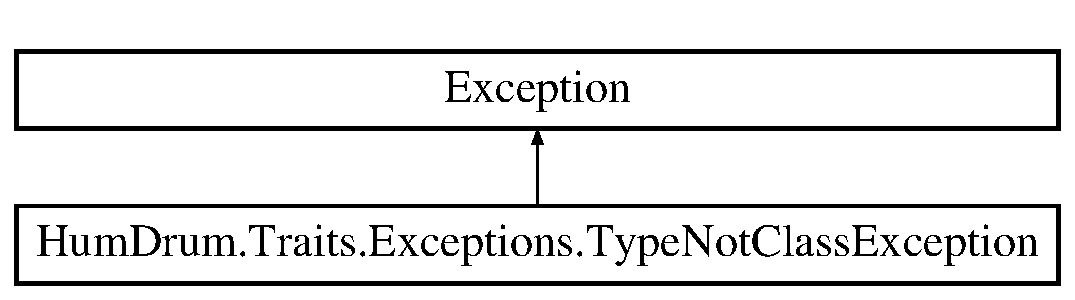
\includegraphics[height=2.000000cm]{classHumDrum_1_1Traits_1_1Exceptions_1_1TypeNotClassException}
\end{center}
\end{figure}
\subsection*{Public Member Functions}
\begin{DoxyCompactItemize}
\item 
\hyperlink{classHumDrum_1_1Traits_1_1Exceptions_1_1TypeNotClassException_a43c3422bfbc73281e5568449f0174cc6}{Type\+Not\+Class\+Exception} ()
\begin{DoxyCompactList}\small\item\em Initializes a new instance of the Hum\+Drum.\+Traits.\+Exceptions+\+Type\+Not\+Class\+Exception class. This will leave the message as \char`\"{}\+Type did not appear to be a class\char`\"{} \end{DoxyCompactList}\item 
\hyperlink{classHumDrum_1_1Traits_1_1Exceptions_1_1TypeNotClassException_a9277bcc94c9f0cf781e613b3aeaa0d23}{Type\+Not\+Class\+Exception} (string message)
\begin{DoxyCompactList}\small\item\em Initializes a new instance of the Hum\+Drum.\+Traits.\+Exceptions+\+Type\+Not\+Class\+Exception class. This gives control over the message \end{DoxyCompactList}\item 
\hyperlink{classHumDrum_1_1Traits_1_1Exceptions_1_1TypeNotClassException_a02ec8aa58b7b3e5f8b30868e047cc62b}{Type\+Not\+Class\+Exception} (string message, Exception inner)
\begin{DoxyCompactList}\small\item\em Initializes a new instance of the Hum\+Drum.\+Traits.\+Exceptions+\+Type\+Not\+Class\+Exception class. This is used when there is an inner exception to throw \end{DoxyCompactList}\end{DoxyCompactItemize}


\subsection{Detailed Description}
Thrown when a type is attempting to be initialized as a \hyperlink{classHumDrum_1_1Traits_1_1Class}{Hum\+Drum.\+Traits.\+Class} but is not declared as a class 



Definition at line 11 of file Exceptions.\+cs.



\subsection{Constructor \& Destructor Documentation}
\index{Hum\+Drum\+::\+Traits\+::\+Exceptions\+::\+Type\+Not\+Class\+Exception@{Hum\+Drum\+::\+Traits\+::\+Exceptions\+::\+Type\+Not\+Class\+Exception}!Type\+Not\+Class\+Exception@{Type\+Not\+Class\+Exception}}
\index{Type\+Not\+Class\+Exception@{Type\+Not\+Class\+Exception}!Hum\+Drum\+::\+Traits\+::\+Exceptions\+::\+Type\+Not\+Class\+Exception@{Hum\+Drum\+::\+Traits\+::\+Exceptions\+::\+Type\+Not\+Class\+Exception}}
\subsubsection[{\texorpdfstring{Type\+Not\+Class\+Exception()}{TypeNotClassException()}}]{\setlength{\rightskip}{0pt plus 5cm}Hum\+Drum.\+Traits.\+Exceptions.\+Type\+Not\+Class\+Exception.\+Type\+Not\+Class\+Exception (
\begin{DoxyParamCaption}
{}
\end{DoxyParamCaption}
)\hspace{0.3cm}{\ttfamily [inline]}}\hypertarget{classHumDrum_1_1Traits_1_1Exceptions_1_1TypeNotClassException_a43c3422bfbc73281e5568449f0174cc6}{}\label{classHumDrum_1_1Traits_1_1Exceptions_1_1TypeNotClassException_a43c3422bfbc73281e5568449f0174cc6}


Initializes a new instance of the Hum\+Drum.\+Traits.\+Exceptions+\+Type\+Not\+Class\+Exception class. This will leave the message as \char`\"{}\+Type did not appear to be a class\char`\"{} 



Definition at line 17 of file Exceptions.\+cs.

\index{Hum\+Drum\+::\+Traits\+::\+Exceptions\+::\+Type\+Not\+Class\+Exception@{Hum\+Drum\+::\+Traits\+::\+Exceptions\+::\+Type\+Not\+Class\+Exception}!Type\+Not\+Class\+Exception@{Type\+Not\+Class\+Exception}}
\index{Type\+Not\+Class\+Exception@{Type\+Not\+Class\+Exception}!Hum\+Drum\+::\+Traits\+::\+Exceptions\+::\+Type\+Not\+Class\+Exception@{Hum\+Drum\+::\+Traits\+::\+Exceptions\+::\+Type\+Not\+Class\+Exception}}
\subsubsection[{\texorpdfstring{Type\+Not\+Class\+Exception(string message)}{TypeNotClassException(string message)}}]{\setlength{\rightskip}{0pt plus 5cm}Hum\+Drum.\+Traits.\+Exceptions.\+Type\+Not\+Class\+Exception.\+Type\+Not\+Class\+Exception (
\begin{DoxyParamCaption}
\item[{string}]{message}
\end{DoxyParamCaption}
)\hspace{0.3cm}{\ttfamily [inline]}}\hypertarget{classHumDrum_1_1Traits_1_1Exceptions_1_1TypeNotClassException_a9277bcc94c9f0cf781e613b3aeaa0d23}{}\label{classHumDrum_1_1Traits_1_1Exceptions_1_1TypeNotClassException_a9277bcc94c9f0cf781e613b3aeaa0d23}


Initializes a new instance of the Hum\+Drum.\+Traits.\+Exceptions+\+Type\+Not\+Class\+Exception class. This gives control over the message 


\begin{DoxyParams}{Parameters}
{\em message} & The text for the Exception\\
\hline
\end{DoxyParams}


Definition at line 27 of file Exceptions.\+cs.

\index{Hum\+Drum\+::\+Traits\+::\+Exceptions\+::\+Type\+Not\+Class\+Exception@{Hum\+Drum\+::\+Traits\+::\+Exceptions\+::\+Type\+Not\+Class\+Exception}!Type\+Not\+Class\+Exception@{Type\+Not\+Class\+Exception}}
\index{Type\+Not\+Class\+Exception@{Type\+Not\+Class\+Exception}!Hum\+Drum\+::\+Traits\+::\+Exceptions\+::\+Type\+Not\+Class\+Exception@{Hum\+Drum\+::\+Traits\+::\+Exceptions\+::\+Type\+Not\+Class\+Exception}}
\subsubsection[{\texorpdfstring{Type\+Not\+Class\+Exception(string message, Exception inner)}{TypeNotClassException(string message, Exception inner)}}]{\setlength{\rightskip}{0pt plus 5cm}Hum\+Drum.\+Traits.\+Exceptions.\+Type\+Not\+Class\+Exception.\+Type\+Not\+Class\+Exception (
\begin{DoxyParamCaption}
\item[{string}]{message, }
\item[{Exception}]{inner}
\end{DoxyParamCaption}
)\hspace{0.3cm}{\ttfamily [inline]}}\hypertarget{classHumDrum_1_1Traits_1_1Exceptions_1_1TypeNotClassException_a02ec8aa58b7b3e5f8b30868e047cc62b}{}\label{classHumDrum_1_1Traits_1_1Exceptions_1_1TypeNotClassException_a02ec8aa58b7b3e5f8b30868e047cc62b}


Initializes a new instance of the Hum\+Drum.\+Traits.\+Exceptions+\+Type\+Not\+Class\+Exception class. This is used when there is an inner exception to throw 


\begin{DoxyParams}{Parameters}
{\em message} & The message to set\\
\hline
{\em inner} & The inner exception\\
\hline
\end{DoxyParams}


Definition at line 38 of file Exceptions.\+cs.



The documentation for this class was generated from the following file\+:\begin{DoxyCompactItemize}
\item 
Hum\+Drum/\+Hum\+Drum/\+Traits/Exceptions.\+cs\end{DoxyCompactItemize}

\hypertarget{classHumDrum_1_1Traits_1_1Exceptions_1_1TypeNotInterfaceException}{}\section{Hum\+Drum.\+Traits.\+Exceptions.\+Type\+Not\+Interface\+Exception Class Reference}
\label{classHumDrum_1_1Traits_1_1Exceptions_1_1TypeNotInterfaceException}\index{Hum\+Drum.\+Traits.\+Exceptions.\+Type\+Not\+Interface\+Exception@{Hum\+Drum.\+Traits.\+Exceptions.\+Type\+Not\+Interface\+Exception}}


Thrown when a type is attempting to be initialized as a \hyperlink{classHumDrum_1_1Traits_1_1Interface}{Hum\+Drum.\+Traits.\+Interface} but appears to not be  


Inheritance diagram for Hum\+Drum.\+Traits.\+Exceptions.\+Type\+Not\+Interface\+Exception\+:\begin{figure}[H]
\begin{center}
\leavevmode
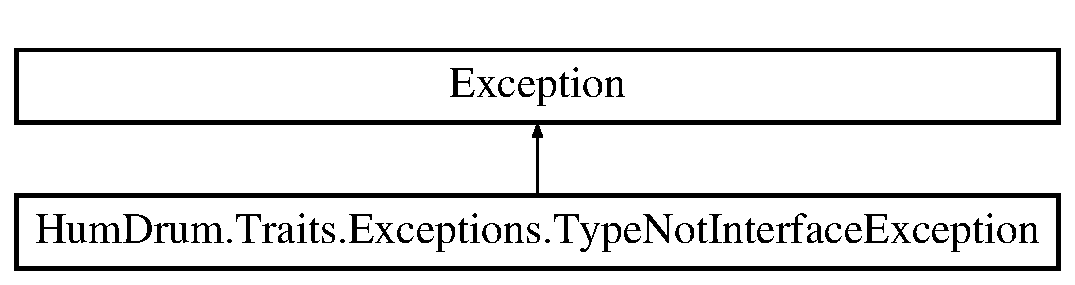
\includegraphics[height=2.000000cm]{classHumDrum_1_1Traits_1_1Exceptions_1_1TypeNotInterfaceException}
\end{center}
\end{figure}
\subsection*{Public Member Functions}
\begin{DoxyCompactItemize}
\item 
\hyperlink{classHumDrum_1_1Traits_1_1Exceptions_1_1TypeNotInterfaceException_a29b2ddfce71c620a9c62087149af2f23}{Type\+Not\+Interface\+Exception} ()
\begin{DoxyCompactList}\small\item\em Initializes a new instance of the Hum\+Drum.\+Traits.\+Exceptions+\+Type\+Not\+Interface\+Exception class. This will leave the message as \char`\"{}\+Type did not appear to be an interface\char`\"{} \end{DoxyCompactList}\item 
\hyperlink{classHumDrum_1_1Traits_1_1Exceptions_1_1TypeNotInterfaceException_afb1f9e4016996d15d225cb0b3fe826c3}{Type\+Not\+Interface\+Exception} (string message)
\begin{DoxyCompactList}\small\item\em Initializes a new instance of the Hum\+Drum.\+Traits.\+Exceptions+\+Type\+Not\+Interface\+Exception class. This gives control over the message \end{DoxyCompactList}\item 
\hyperlink{classHumDrum_1_1Traits_1_1Exceptions_1_1TypeNotInterfaceException_a0af1718df1e02150029bad6dbaec3ade}{Type\+Not\+Interface\+Exception} (string message, Exception inner)
\begin{DoxyCompactList}\small\item\em Initializes a new instance of the Hum\+Drum.\+Traits.\+Exceptions+\+Type\+Not\+Interface\+Exception class. This is used when there is an inner exception to throw \end{DoxyCompactList}\end{DoxyCompactItemize}


\subsection{Detailed Description}
Thrown when a type is attempting to be initialized as a \hyperlink{classHumDrum_1_1Traits_1_1Interface}{Hum\+Drum.\+Traits.\+Interface} but appears to not be 



Definition at line 48 of file Exceptions.\+cs.



\subsection{Constructor \& Destructor Documentation}
\index{Hum\+Drum\+::\+Traits\+::\+Exceptions\+::\+Type\+Not\+Interface\+Exception@{Hum\+Drum\+::\+Traits\+::\+Exceptions\+::\+Type\+Not\+Interface\+Exception}!Type\+Not\+Interface\+Exception@{Type\+Not\+Interface\+Exception}}
\index{Type\+Not\+Interface\+Exception@{Type\+Not\+Interface\+Exception}!Hum\+Drum\+::\+Traits\+::\+Exceptions\+::\+Type\+Not\+Interface\+Exception@{Hum\+Drum\+::\+Traits\+::\+Exceptions\+::\+Type\+Not\+Interface\+Exception}}
\subsubsection[{\texorpdfstring{Type\+Not\+Interface\+Exception()}{TypeNotInterfaceException()}}]{\setlength{\rightskip}{0pt plus 5cm}Hum\+Drum.\+Traits.\+Exceptions.\+Type\+Not\+Interface\+Exception.\+Type\+Not\+Interface\+Exception (
\begin{DoxyParamCaption}
{}
\end{DoxyParamCaption}
)\hspace{0.3cm}{\ttfamily [inline]}}\hypertarget{classHumDrum_1_1Traits_1_1Exceptions_1_1TypeNotInterfaceException_a29b2ddfce71c620a9c62087149af2f23}{}\label{classHumDrum_1_1Traits_1_1Exceptions_1_1TypeNotInterfaceException_a29b2ddfce71c620a9c62087149af2f23}


Initializes a new instance of the Hum\+Drum.\+Traits.\+Exceptions+\+Type\+Not\+Interface\+Exception class. This will leave the message as \char`\"{}\+Type did not appear to be an interface\char`\"{} 



Definition at line 54 of file Exceptions.\+cs.

\index{Hum\+Drum\+::\+Traits\+::\+Exceptions\+::\+Type\+Not\+Interface\+Exception@{Hum\+Drum\+::\+Traits\+::\+Exceptions\+::\+Type\+Not\+Interface\+Exception}!Type\+Not\+Interface\+Exception@{Type\+Not\+Interface\+Exception}}
\index{Type\+Not\+Interface\+Exception@{Type\+Not\+Interface\+Exception}!Hum\+Drum\+::\+Traits\+::\+Exceptions\+::\+Type\+Not\+Interface\+Exception@{Hum\+Drum\+::\+Traits\+::\+Exceptions\+::\+Type\+Not\+Interface\+Exception}}
\subsubsection[{\texorpdfstring{Type\+Not\+Interface\+Exception(string message)}{TypeNotInterfaceException(string message)}}]{\setlength{\rightskip}{0pt plus 5cm}Hum\+Drum.\+Traits.\+Exceptions.\+Type\+Not\+Interface\+Exception.\+Type\+Not\+Interface\+Exception (
\begin{DoxyParamCaption}
\item[{string}]{message}
\end{DoxyParamCaption}
)\hspace{0.3cm}{\ttfamily [inline]}}\hypertarget{classHumDrum_1_1Traits_1_1Exceptions_1_1TypeNotInterfaceException_afb1f9e4016996d15d225cb0b3fe826c3}{}\label{classHumDrum_1_1Traits_1_1Exceptions_1_1TypeNotInterfaceException_afb1f9e4016996d15d225cb0b3fe826c3}


Initializes a new instance of the Hum\+Drum.\+Traits.\+Exceptions+\+Type\+Not\+Interface\+Exception class. This gives control over the message 


\begin{DoxyParams}{Parameters}
{\em message} & The text for the Exception\\
\hline
\end{DoxyParams}


Definition at line 64 of file Exceptions.\+cs.

\index{Hum\+Drum\+::\+Traits\+::\+Exceptions\+::\+Type\+Not\+Interface\+Exception@{Hum\+Drum\+::\+Traits\+::\+Exceptions\+::\+Type\+Not\+Interface\+Exception}!Type\+Not\+Interface\+Exception@{Type\+Not\+Interface\+Exception}}
\index{Type\+Not\+Interface\+Exception@{Type\+Not\+Interface\+Exception}!Hum\+Drum\+::\+Traits\+::\+Exceptions\+::\+Type\+Not\+Interface\+Exception@{Hum\+Drum\+::\+Traits\+::\+Exceptions\+::\+Type\+Not\+Interface\+Exception}}
\subsubsection[{\texorpdfstring{Type\+Not\+Interface\+Exception(string message, Exception inner)}{TypeNotInterfaceException(string message, Exception inner)}}]{\setlength{\rightskip}{0pt plus 5cm}Hum\+Drum.\+Traits.\+Exceptions.\+Type\+Not\+Interface\+Exception.\+Type\+Not\+Interface\+Exception (
\begin{DoxyParamCaption}
\item[{string}]{message, }
\item[{Exception}]{inner}
\end{DoxyParamCaption}
)\hspace{0.3cm}{\ttfamily [inline]}}\hypertarget{classHumDrum_1_1Traits_1_1Exceptions_1_1TypeNotInterfaceException_a0af1718df1e02150029bad6dbaec3ade}{}\label{classHumDrum_1_1Traits_1_1Exceptions_1_1TypeNotInterfaceException_a0af1718df1e02150029bad6dbaec3ade}


Initializes a new instance of the Hum\+Drum.\+Traits.\+Exceptions+\+Type\+Not\+Interface\+Exception class. This is used when there is an inner exception to throw 


\begin{DoxyParams}{Parameters}
{\em message} & The message to set\\
\hline
{\em inner} & The inner exception\\
\hline
\end{DoxyParams}


Definition at line 75 of file Exceptions.\+cs.



The documentation for this class was generated from the following file\+:\begin{DoxyCompactItemize}
\item 
Hum\+Drum/\+Hum\+Drum/\+Traits/Exceptions.\+cs\end{DoxyCompactItemize}

%--- End generated contents ---

% Index
\backmatter
\newpage
\phantomsection
\clearemptydoublepage
\addcontentsline{toc}{chapter}{Index}
\printindex

\end{document}
